\documentclass[aspectratio=169]{beamer}

\usepackage[utf8]{inputenc}
%\usepackage{emoji}

\usepackage{amsmath}
\usepackage{graphicx}
\usepackage[T1]{fontenc}
\usepackage{libertine}
\usepackage{array}
\usepackage{enumitem}
\usepackage{marvosym}

\setitemize{label=\usebeamerfont*{itemize item}%
  \usebeamercolor[fg]{itemize item}
  \usebeamertemplate{itemize item},
}
\setbeamertemplate{itemize item}[square]
\setbeamertemplate{itemize subitem}[circle]

\usepackage{pgfplots}
\usepackage{tikz}
\usetikzlibrary{automata, arrows, positioning, calc, external, babel, backgrounds, matrix, shapes, shadings}
\usepgfplotslibrary{fillbetween}


%%natbib conf
\usepackage[square,authoryear]{natbib}
\renewcommand{\cite}{\citep}
\renewcommand{\bibfont}{\small}
\bibliographystyle{abbrvnat} 

\newcommand{\R}{\mathbb{R}}
\newcommand{\brackets}[2]{\left\langle#1,#2\right\rangle}
\newcommand{\ind}[1]{\mathbf{1}_{\left\{#1\right\}}}

\newcommand{\graphheight}{7cm}
\newcommand{\graphwidth}{11cm}

\newcommand{\E}[1]{E\left[#1 \right]}
\renewcommand{\phi}{\varphi}

% \definecolor{azulcito}{RGB}{20,70,140}
\definecolor{azulcito}{RGB}{0,90,150}
\definecolor{verdecito}{RGB}{90,150,0}
\definecolor{rojito}{RGB}{150,0,90}
\definecolor{violetita}{RGB}{150,20,150}


\setbeamercolor*{structure}{fg=azulcito,bg=azulcito!20!white}
\setbeamercolor*{alerted text}{fg=azulcito}

  \setbeamercolor{block title}{fg=azulcito,bg=azulcito!20!white}
  \setbeamercolor{block body}{fg=black,bg=azulcito!10!white}
  
\beamertemplatenavigationsymbolsempty

\setbeamercolor*{author in head/foot}{fg=azulcito,bg=azulcito!15!white}
\setbeamercolor*{title in head/foot}{fg=azulcito,bg=azulcito!15!white}
\setbeamercolor*{date in head/foot}{fg=azulcito,bg=azulcito!15!white}

% Pgfplots
\pgfplotsset{width=\graphwidth, height = \graphheight, grid style = {dashed, gray}, every tick label/.append style = {font=\footnotesize}, compat=1.18, legend style={font=\footnotesize, draw=none, fill=none}, every axis/.append style={label style={font=\footnotesize}}}

\tikzset{>=stealth}

\newtheorem{proposition}{Proposition}
%\newtheorem{definition}{Definition}
%\newtheorem{lemma}{Lemma}
%\newtheorem{corollary}{Corollary}

\defbeamertemplate*{footline}{mitema}
{
  \leavevmode%
  \hbox{%
  \begin{beamercolorbox}[wd=.25\paperwidth,ht=2.25ex,dp=1ex,left]{author in head/foot}%
    \usebeamerfont{author in head/foot}\hspace*{2ex}\insertshortauthor
  \end{beamercolorbox}%
  \begin{beamercolorbox}[wd=.5\paperwidth,ht=2.25ex,dp=1ex,center]{title in head/foot}%
    \usebeamerfont{date in head/foot}\insertshortdate{}
  \end{beamercolorbox}%
  \begin{beamercolorbox}[wd=.25\paperwidth,ht=2.25ex,dp=1ex,right]{date in head/foot}%
    \insertframenumber{}/\inserttotalframenumber\hspace*{2em} 
  \end{beamercolorbox}}%
 \vskip0pt%
}


\setbeamercolor{blocky}{fg=azulcito,bg=azulcito!15!white}
\setbeamercolor{blocky2}{fg=black,bg=azulcito!10!white}

\defbeamertemplate*{title page}{customized}[1][]
{
{\flushright
  \begin{beamercolorbox}[wd=\paperwidth,sep=1em,right,rightskip=1.5em]{blocky}%
    \usebeamerfont{title}{\huge \inserttitle}\par \bigskip

    \usebeamerfont{subtitle}{\large \insertsubtitle}\par
  \end{beamercolorbox}%
  \vfill
    \usebeamerfont{author}{\Large \insertauthor}\par \vspace{1em}
      \usebeamerfont{institute}{\large \insertinstitute}\par
  
  
  \vfill
  \usebeamerfont{date}{\insertdate}\par
  %\usebeamercolor[fg]{titlegraphic}\inserttitlegraphic
  }
}

\usefonttheme[onlymath]{serif}

\title{The last, the least and the urgent...}
\subtitle{Fluid modeling and performance equivalence for scheduling policies in partial service queues with abandonment}

\author[Andres Ferragut, Universidad ORT Uruguay]{Andres Ferragut}
\institute{with Diego Goldsztajn y Fernando Paganini}
\date[IFIP Performance 2025 -- Amsterdam -- November 2025]{IFIP Performance 2025}

\AtBeginSection[]
{
\begin{frame}{Outline}
\tableofcontents[currentsection, 
   hideallsubsections, 
   sectionstyle=show/shaded,
]
\end{frame}
}

\newenvironment*{myitem}[1][1.5em]{\begin{itemize}\setlength{\itemsep}{#1}}{\end{itemize}}

\begin{document}

\frame[plain]{\titlepage}

\begin{frame}{Outline}
\tableofcontents
\end{frame}

\section{Introduction}

\begin{frame}{Motivation}{A bit of history...}

	\begin{myitem}
		\item Several queueing systems have service and \alert{timing} requirements.
		\item Examples:
		\begin{itemize}
			\item Computing tasks with real-time constraints.
			\item Item delivery problems in logistics.
			\item Emergency response.
			\item etc. etc. etc.
		\end{itemize}
		\item This has led to a long and rich history of research about \alert{queues with abandonments} \cite{barrer1957queuing,stanford1979reneging,baccellietal1984single}.
	\end{myitem}

\end{frame}

\begin{frame}{Motivation}{Recent developments...}

	One of the most used policies is \alert{Earliest-Deadline-First (EDF)}
	\begin{itemize}
		\item Give priority to tasks with more urgent deadlines.
	\end{itemize}
	\vfill
	\pause
	
	Through fluid limits and diffusion approximations, establish performance:
	\begin{itemize}
		\item \cite{decreusefondmoyal2005fluid} establish EDF fluid limits in the single server case.
		\item \cite{kruketal2011heavy} provides diffusion approximations.
		\item \cite{moyal2013queues} establish some optimality properties of EDF.
		\item \cite{kangramanan2010fluid, kangramanan2012asymptotic} analyze the many-server case.
		\item \cite{ataretal2018law,ataretal2023long} establish asymptotic performance.
	\end{itemize}
	\vfill
	and many others...
\end{frame}

\begin{frame}{Motivation}
	
	\begin{block}{Common assumption}
		\begin{center}
		Customers renege \emph{only} in the queue, and not during service.
		\end{center}
	\end{block}
	\vfill
	\pause

	We call this the \emph{call-center scenario}:

	\begin{itemize}
		\item Akin to waiting for the customer-help line to pick your call while you listen to annoying music.
		
		\item The underlying idea is that when a task reaches service, it will stay until completion.
		
	\end{itemize}
	
	\vfill

	\alert{Key performance metric:} number of satisfied tasks (or reneging probability).

\end{frame}

\begin{frame}{Motivation}{Partial service queues}

	In several queueing systems:

	\begin{itemize}
		\item Tasks may abandon during service.
		\item More importantly, \alert{all service provided may be useful}.
	\end{itemize}

	\vfill

	We call this setting \alert{queues with partial service}.

	\pause

	\vfill

	Some examples:
	\begin{itemize}
		\item Electrical vehicle charging: customers leave the system with a \emph{partial charge}.
		\item LLM inference: longer computation times lead to better answers, but these may be interrupted to deliver a quick response.
		\item File transfers over the Internet, that can be resumed later.
	\end{itemize}

\end{frame}

\begin{frame}{Key points of this talk}
	
	\begin{myitem}
		\item Provide some suitable representation of the state space and dynamics of these partial service queues.
		
		\item Analyze several interesting policies under a suitable fluid model.
		
		\item Compute the main performance metric here: \alert{attained work}.
		
		\item \emph{Last but not least:} show that the simple LCFS policy \alert{exhibits the same performance} than EDF in this setting, without using deadline information. 
	\end{myitem}
\end{frame}

% \section{A crash course on measure valued processes}

% \begin{frame}{Measure valued stochastic processes}
	
% 	Consider the simple $M/G/\infty$ queue:
% 	\begin{itemize}
% 		\item Tasks arrive as a Poisson process of intensity $\lambda$.
% 		\item Each task has a service requirement $S\sim g(\sigma)$.
% 	\end{itemize}
% 	\vfill
% 	\begin{center}
% 		\begin{tikzpicture}    
% 			\draw [->] (-.2,0) -- node[midway,below,yshift=-1ex]{\footnotesize Remaining service} (7,0);
% 			\node [below right] at (7,0) {$\sigma$};
% 			\draw (0,.1) -- (0,-.1) node[below] {$0$};

% 			\uncover<2>{
% 				\draw [->,rojito] (6,1) node[above] {New mass arrives, rate $\lambda g(\sigma)d\sigma dt$} -- (6,.1);
% 				\draw [rojito, fill=rojito] (6,0) circle [radius=0.1];
% 			}
% 			\uncover<3>{
% 				\draw [azulcito, fill=azulcito] (6,0) circle [radius=0.1];
% 				\draw [thick,->] (6,.2) -- node[midway,above,yshift=1ex] {Drifts to the left ar rate $1$} ++(-.3,0);
% 			}
% 			\uncover<4>{
% 				\draw [azulcito, fill=azulcito, opacity = 0.5, fill opacity=0.5] (0,0) circle [radius=0.1];
% 				\node[azulcito] at (0.2,0.5) {\Huge\Lightning};
% 				\node[azulcito] at (1,1.1) {Departure};
% 			}
% 			\uncover<5->{
% 				\foreach \x in {.5,.8,2,2.5,3.7,4.3,5,5.5} {
% 					\draw [azulcito, fill=azulcito] (\x,0) circle [radius=0.1];
% 					\draw<5> [thick,->] (\x,.2) --  ++(-.3,0);
% 				}
% 				\node at (3.5,1) {Steady-state};
% 			}

			
% 		\end{tikzpicture}
% 	\end{center}
% 	\vfill
% 	\uncover<6->{
% 		\alert{State-descriptor:}
% 		\begin{equation*}
% 			\Phi_t = \sum_i \delta_{\sigma_i(t)}
% 		\end{equation*}
% 		a Point-process on the positive half-line.
% 	}
% \end{frame}

% \begin{frame}{M/G/$\infty$, steady state}
	
% 	\begin{itemize}
% 		\item $\Phi_t$ is a measure-valued Markov process.
% 		\item Its dynamics can be characterized through its generator.
% 		\item In steady state:
% 		\begin{equation*}
% 			\Phi \sim \textrm{Poisson Process with mean measure } \mu(d\sigma) = \lambda \bar{G}(\sigma)d\sigma
% 		\end{equation*}
% 		where $\bar{G}$ is the CCDF of $S$.
% 	\end{itemize}

% 	\pause
% 	\vfill
% 	\alert{Interpretation:}

% 	\begin{itemize}
% 	 \item Write $\mu(d\sigma) = \rho \left[\frac{1}{E[S]}(1-G(\sigma))\right]d\sigma$, with $\rho = \lambda E[S]$.
% 	 \item Then $\left[\frac{1}{E[S]}(1-G(\sigma))\right]d\sigma$ is the \emph{residual service time distribution} associated to $G$.
% 	 \item In steady-state, the total number of customers $\sim \textrm{Poisson}(\rho)$ and distributed in $\sigma$ as the residual lifetime distribution.
% 	\end{itemize}

% \end{frame}

% \begin{frame}{M/G/$\infty$, fluid approximation.}
	
% 	Suppose that we can replace $\Phi_t$ by a general measure $\mu_t$ with density $f(\sigma;t)$. 
	
% 	\begin{center}
% 		\begin{tikzpicture}    
% 			\draw [->] (-.2,0) -- node[midway,below,yshift=-1ex]{\footnotesize Remaining service} (7,0);
% 			\node [below right] at (7,0) {$\sigma$};
% 			\draw (0,.1) -- (0,-.1) node[below] {$0$};

% 			\draw [azulcito, very thick] plot [smooth] coordinates {(0,2) (2,1) (3,.8) (4,.5) (5,.3) (6,.1)};
% 			\node[azulcito] at (4,1) {$f(\sigma;t)$};
% 		\end{tikzpicture}
% 	\end{center}
% 	\begin{itemize}
% 		\item Mass is transported to the left at rate $1$.
% 		\item New mass arrives at $\sigma$ with intensity $\lambda g(\sigma)d\sigma dt$.
% 	\end{itemize}
% \vfill
% 	We can combine this in the following \alert{transport equation}:
% 	\begin{equation*}
% 		\frac{\partial f}{\partial t} = \frac{\partial f}{\partial \sigma} + \lambda g(\sigma).
% 	\end{equation*}

% \end{frame}

% \begin{frame}{M/G/$\infty$, fluid approximation.}

% 	Imposing equilibrium and the boundary condition $f(\sigma)\to 0$ as $\sigma\to\infty$ we get:
% 	\begin{equation*}
% 		\frac{\partial f}{\partial \sigma} + \lambda g(\sigma) = 0 \Longrightarrow f(\sigma) = \lambda \int_\sigma^{\infty} g(u)\, du = \lambda \bar{G}(\sigma),
% 	\end{equation*}
% 	so the fluid approximation recovers the mean measure of $\Phi$.

% 	\pause\vfill
% 	\begin{itemize}
% 		\item This is a deterministic measure, with total mass $\rho$... 
% 		\item ...distributed in the real line as the residual service distribution.
% 		\item Serves as an approximation of $\Phi$ in a large scale system ($\lambda\to\infty$).
% 	\end{itemize}
% \end{frame}

% \begin{frame}{M/G/$\infty$: take two}{Attained service state descriptor}

% 	Here is another approach to model the same system \cite{kangramanan2010fluid}:
% 	\vfill
% 	\begin{center}
% 		\begin{tikzpicture}    
% 			\draw [->] (-.2,0) -- node[midway,below,yshift=-1ex]{\footnotesize Attained service} (7,0);
% 			\node [below right] at (7,0) {$x$};
% 			\draw (0,.1) -- (0,-.1) node[below] {$0$};

% 			\uncover<2>{
% 				\draw [->,rojito] (0,1) node[above] {New mass arrives, rate $\lambda dt$} -- (0,.1);
% 				\draw [rojito, fill=rojito] (0,0) circle [radius=0.1];
% 			}
% 			\uncover<3>{
% 				\draw [azulcito, fill=azulcito] (0,0) circle [radius=0.1];
% 				\draw [thick,->] (0,.2) -- node[midway,above,yshift=1ex] {Drifts to the right ar rate $1$} ++(.3,0);
% 			}
% 			\uncover<4>{
% 				\draw [azulcito, fill=azulcito, opacity = 0.5, fill opacity=0.5] (5,0) circle [radius=0.1];
% 				\node[azulcito] at (5.2,0.5) {\Huge\Lightning};
% 				\node[azulcito] at (5,1.1) {Departure when $S$ expires};
% 			}
% 			\uncover<5->{
% 				\foreach \x in {.5,.8,2,2.5,3.7,4.3,5,5.5} {
% 					\draw [azulcito, fill=azulcito] (\x,0) circle [radius=0.1];
% 					\draw<5> [thick,->] (\x,.2) --  ++(.3,0);
% 				}
% 				\node at (3.5,1) {Steady-state};
% 			}

			
% 		\end{tikzpicture}
% 	\end{center}
% 	\vfill
% 	\uncover<6->{
% 		\alert{State-descriptor:}
% 		\begin{equation*}
% 			\tilde{\Phi}_t = \sum_i \delta_{x_i(t)}
% 		\end{equation*}
% 		a Point-process on the positive half-line, where $x_i(t)$ is the elapsed time in the system
% 	}

% \end{frame}

% \begin{frame}{M/G/$\infty$, take two}{Steady-state}
	
% 	$\tilde\Phi_t$ is a measure-valued Markov process.

% 	\begin{itemize}
% 		\item Mass always arrive at $0$ with rate $\lambda dt$.
% 		\item Transports to the right at rate $1$.
% 		\item Leaves the system at rate $h(x)$, the \alert{hazard rate function}:
% 		\begin{equation*}
% 			h(x) = \lim_{dt\to 0} P(S\in[x,x+dt]\mid S>x) = \frac{g(x)}{\bar{G}(x)} = -\frac{\partial}{\partial x} \log \bar{G}(x).
% 		\end{equation*}
% 	\end{itemize}

% 	\pause
% 	\vfill
% 	\alert{Steady-state:}
% 		\begin{equation*}
% 			\tilde\Phi \sim \textrm{Poisson Process with mean measure } \nu(dx) = \lambda \bar{G}(x)dx
% 		\end{equation*}
	
	
% 	\vfill

% 	So the reversed representation has the same distribution, because in a random point in time the elapsed service and the remaining service have the same distribution.

% \end{frame}


% \begin{frame}{M/G/$\infty$: take two}{Fluid approximation.}
	
% 	Suppose that we can replace $\tilde\Phi_t$ by a general measure $\nu_t$ with density $\tilde f(x;t)$. 
	
% 	\begin{center}
% 		\begin{tikzpicture}    
% 			\draw [->] (-.2,0) -- node[midway,below,yshift=-1ex]{\footnotesize Attained service} (7,0);
% 			\node [below right] at (7,0) {$x$};
% 			\draw (0,.1) -- (0,-.1) node[below] {$0$};

% 			\draw [azulcito, very thick] plot [smooth] coordinates {(0,2) (2,1) (3,.8) (4,.5) (5,.3) (6,.1)};
% 			\node[azulcito] at (4,1) {$\tilde f(x;t)$};
% 		\end{tikzpicture}
% 	\end{center}
% \vfill
% \pause
% The corresponding transport equation is (informally):
% 	\begin{equation*}
% 		\frac{\partial \tilde f}{\partial t} = -\frac{\partial \tilde f}{\partial x} - h(x)\tilde{f} + \lambda \delta_0.
% 	\end{equation*}
% \end{frame}

% \begin{frame}{M/G/$\infty$: take two}{Fluid equilibrium.}
	
% Imposing equilibrium we get:
% 	\begin{equation*}
% 		\frac{\partial \tilde f}{\partial x} = - h(x)\tilde{f} + \lambda \delta_0.
% 	\end{equation*}

% Solving (in a distribution sense) with the boundary condition $\tilde f (\infty) = 0$ we get:
% 	\begin{equation*}
% 		\tilde{f}(x) = \lambda e^{-\int_0^x h(u)du}.
% 	\end{equation*}

% But by definition $\int_0^x h(u) du = -\log \bar{G}(x)$, and thus:
% 	\begin{equation*}
% 		\tilde{f}(x) = \lambda \bar{G}(x)
% 	\end{equation*}

% So the transport fluid equation recovers again the mean measure of the steady-state.

% \end{frame}

% \begin{frame}{Lessons learned}

% 	\begin{myitem}
% 		\item We can model $M/G$ systems by using two state descriptors:
% 			\begin{itemize}
% 				\item The remaining service $\Phi$.
% 				\item The attained service $\tilde\Phi$.
% 			\end{itemize}
% 		\item Both admit reasonable fluid approximations, which correspond to transport equations.
% 		\item In fact this has been used in the literature to model abandonments (since they operate as $M/G/\infty$ systems in some sense).
% 	\end{myitem}
% 	\pause \vfill
% 	\alert{Question:} can we do more using this machinery of measure-valued processes?
% \end{frame}

\section{Partial service queues}

\begin{frame}{Setting}

	Consider an $M/G/C$ system where:
	\begin{columns}
		\begin{column}{0.5\textwidth}
			\begin{itemize}
			\item Tasks arrive as a Poisson process of intensity $\lambda$.
			\item<2-> Each task $i$ has two characteristics (marks):
			\begin{itemize}
				\item $S_i$: service time (at rate $1$).
				\item $T_i$: sojourn time or deadline.
			\end{itemize}
			\item<3-> $(S_i,T_i)$ are independent across jobs.
			\item<3-> Follow a common distribution $G(\sigma,\tau)$, possibly correlated.
			\end{itemize} 
		\end{column}
		\begin{column}{0.5\textwidth}

			\begin{tikzpicture}
				\node (arrival) at (0,0) {$\lambda$};
				\node [right of=arrival] (queuel) {};
				\draw[->] (arrival) -- (queuel);
				\draw[thick] (queuel)++(0,.6) --node[midway,above] {Queue} ++(3,0) -- ++(0,-1.2) -- ++(-3,0);

				\foreach \x in {2,2.4,2.8,3.2,3.6} {
					\fill[rojito,thick, fill=rojito!70!white] (\x,.5) rectangle ++(.3,-1);
				}
				\foreach \y in {2,1,0,-1,-2} {
					\draw[azulcito, thick, fill=azulcito!70!white] (5,\y) circle [radius=.4];
				}
				\node[above] at (5,2.5) {$C$ servers};

				\draw<2->[thick,rojito] (2.5,-.75) rectangle ++(1,-1.6);
				\node<2-> at (3,-1.2) {\includegraphics[width=.5cm]{figuras/battery_mid.png}};
				\node<2-> at (3,-2) {\includegraphics[width=.5cm]{figuras/clock.png}};

				\draw<2->[rojito,thick,->] (2.15,-.5) -- (2.15,-1.6) -- (2.5,-1.6);
			\end{tikzpicture}

		\end{column}
	\end{columns}
\end{frame}

\begin{frame}{Partial service queues}{Definition}

	\begin{block}{Partial service queue}
		Customers depart whenever $S_i$ is attained or the timer $T_i$ expires.
	\end{block}
	\vfill

	\pause
	\begin{myitem}
		\item In particular, they may leave \alert{during service}.

		\item Key performance metrics:
		\begin{myitem}[1em]
			\item \alert{$S_a$}: amount of service \alert{attained}.
			\item Equivalently, \alert{$S_r$}$:=S-S_a$, amount of service \alert{reneged}. 
		\end{myitem}

		\pause

		\item \alert{Problem:} we have to keep track of remaining service and deadlines simultaneously!
	\end{myitem}
\end{frame}


\begin{frame}{System load}

	\begin{myitem}
		
	\item Before proceeding, it is useful to define the \alert{system load}:

	\begin{equation*}
		\rho:= \lambda E[\min\{S,T\}].
	\end{equation*}

	\pause

	\item \alert{Interpretation:} the mean number of customers on a system with $C=\infty$.

	\item What we expect in a large scale fluid model:
	
	\begin{itemize}
	 \item If $\rho<C$ (underload), all tasks can be served, $S_a = \min\{S,T\}$.
	 \item If $\rho>C$ (overload), demand \emph{curtailing} will occur. How? It depends on the policy...
	\end{itemize}

	\end{myitem}


\end{frame}

\begin{frame}{System evolution}{Remaining service times}

	\begin{columns}
	\begin{column}{0.45\textwidth}
		  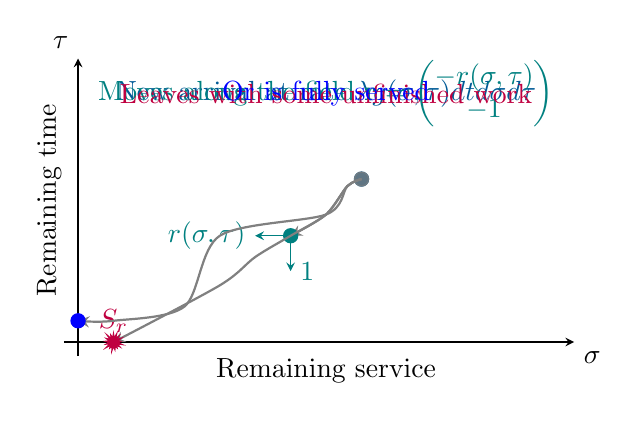
\begin{tikzpicture}[scale=0.9]
    
			\draw [->] (-.2,0) -- (7,0);
			\node [below right] at (7,0) {$\sigma$};
			\draw [->] (0,-.2) -- (0,4);
			\node [above left] at (0,4) {$\tau$};
			
			\node [below] at (3.5,-.1) {Remaining service};
			\node [rotate=90, left, anchor=south] at (-.1,2) {Remaining time};
			
			%	\draw [thick,gray,->] (4,2.3) -- ++(0,-.4);
			\draw<2> [azulcito, fill=azulcito] (4,2.3) circle [radius=0.1];
			\node<2> [azulcito] at (3.5,3.5) {New arrival at rate $\lambda g(\sigma,\tau)dtd\sigma d\tau$};

			\draw<3> [thick,gray,->] plot[smooth] coordinates {(4,2.3) (3.8,2.2) (3.5,1.8) (3,1.5)}; 
			\draw<3> [gray, fill=gray, opacity=0.5] (4,2.3) circle [radius=0.1];
			\draw<3> [teal, fill=teal] (3,1.5) circle [radius=0.1];
			\draw<3> [teal, fill=teal,->] (3,1.5) -- (2.5,1.5) node[left]{$r(\sigma,\tau)$};
			\draw<3> [teal, fill=teal,->] (3,1.5) -- (3,1) node[right]{$1$};
			\node<3> [teal] at (3.5,3.5) {Moves along the field $\mathbf{r} = \begin{pmatrix}
			-r(\sigma,\tau) \\ -1
			\end{pmatrix}$};

			\draw<4> [thick,gray,->] plot[smooth] coordinates {(4,2.3) (3.8,2.2) (3.5,1.8) (3,1.5) (2.5,1.2) (2,.8) (.5,0)}; 
			\draw<4-5> [gray, fill=gray, opacity=0.5] (4,2.3) circle [radius=0.1];
			\node<4>[purple, fill=purple, starburst, inner sep=1.5pt,/pgf/starburst point height=3] at (.5,0) {};
			\node<4>[purple,above] at (.5,0) {$S_r$};
			\node<4> [purple] at (3.5,3.5) {Leaves with some unfinished work};

			\draw<5> [thick,gray,->] plot[smooth] coordinates {(4,2.3) (3.8,2.2) (3.5,1.8) (2,1.5) (1.5,.5) (.5,.3) (0,.3)}; 
			\draw<5> [blue, fill=blue] (0,.3) circle [radius=0.1];
			\node<5> [blue] at (3.5,3.5) {Or is fully served};

		\end{tikzpicture}

	\end{column}
	\begin{column}{0.55\textwidth}
		\begin{itemize}
			\item<1-> Consider the remaining time space.
			\item<3-> \alert{Policy} defines how tasks are served.
			\item<3-> May depend on any combination of $(\sigma,\tau)$.
			\item<5-> State descriptor:
			 \begin{equation*}
				\Phi_t = \sum_i \delta_{\left(\sigma_i(t),\tau_i(t)\right)}
			 \end{equation*}
		\end{itemize}
	\end{column}
	\end{columns}

\end{frame}

\begin{frame}{Example: Earliest-deadline-first}

	\begin{columns}
		\begin{column}{0.45\textwidth}
		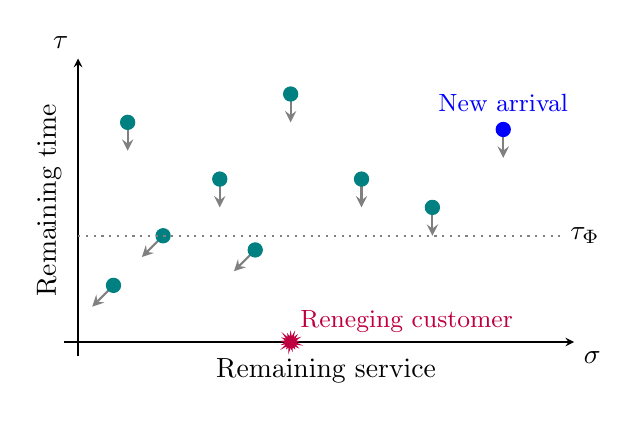
\begin{tikzpicture}[scale=0.9]
				
			\draw [->] (-.2,0) -- (7,0);
			\node [below right] at (7,0) {$\sigma$};
			\draw [->] (0,-.2) -- (0,4);
			\node [above left] at (0,4) {$\tau$};
			
			\node [below] at (3.5,-.1) {Remaining service};
			\node [rotate=90, left, anchor=south] at (-.1,2) {Remaining time};
			
			\draw [thick,gray,->] (.5,.8) -- ++(-.3,-.3);
			\draw [thick,gray,->] (.7,3.1) -- ++(0,-.4);
			\draw [thick,gray,->] (1.2,1.5) -- ++(-.3,-.3);
			\draw [thick,gray,->] (2,2.3) -- ++(0,-.4);
			\draw [thick,gray,->] (2.5,1.3) -- ++(-.3,-.3);
			\draw [thick,gray,->] (3,3.5) -- ++(0,-.4);
			\draw [thick,gray,->] (4,2.3) -- ++(0,-.4);
			\draw [thick,gray,->] (5,1.9) -- ++(0,-.4);
			\draw [thick,gray,->] (6,3) -- ++(0,-.4);

			\draw [teal, fill=teal] (.5,.8) circle [radius=0.1];
			\draw [teal, fill=teal] (.7,3.1) circle [radius=0.1];
			\draw [teal, fill=teal] (1.2,1.5) circle [radius=0.1];
			\draw [teal, fill=teal]  (2,2.3) circle [radius=0.1];
			\draw [teal, fill=teal] (2.5,1.3) circle [radius=0.1];
			\draw [teal, fill=teal] (3,3.5) circle [radius=0.1];
			\draw [teal, fill=teal] (4,2.3) circle [radius=0.1];
			\draw [teal, fill=teal] (5,1.9) circle [radius=0.1];
			\draw [blue, fill=blue] (6,3) circle [radius=0.1] node[above, yshift=3pt] {\small New arrival};

			%reneging departure
			%\draw [purple, fill=purple!20!white] (3,0) circle [radius=0.1] node[above, anchor=south west] {\small Reneging customer};
			\node[purple, fill=purple, starburst, inner sep=1.5pt,/pgf/starburst point height=3] at (3,0) {};
			\node[purple, anchor=south west] at (3,0){ \small Reneging customer};

			\draw [gray, dotted, thick] (0,1.5) -- (6.8,1.5) node[black, right] {$\tau_\Phi$};

		\end{tikzpicture}
	\end{column}
	\begin{column}{0.55\textwidth}
		\begin{itemize}
			\item Serve the $C$ most urgent customers.
			\item Corresponds to taking:
				\begin{equation*}
					r_\Phi(\sigma,\tau) = \mathbf{1}_{\{\tau\leqslant\tau_\Phi\}} 
				\end{equation*}
				with
				\begin{equation*} 
					\tau_\Phi := \sup\{\tau \geqslant 0: \Phi(\mathbb{R}_{+} \times (0, \tau]) < C\}. 	
				\end{equation*} 
		\end{itemize}
	\end{column}
\end{columns}
\end{frame}


\begin{frame}{Fluid model dynamics}
	\begin{itemize}
		\item Replace $\Phi_t$ by a (fluid) measure $\mu_t$.
		\item Now mass drifts along the field:
			\begin{equation*}
				\mathbf{r}_\mu(\sigma,\tau) = \begin{pmatrix}
				-r_\mu(\sigma,\tau) \\
				-1
				\end{pmatrix}
 			\end{equation*}
		\item With $r_\mu$ satisfying:
		\begin{gather*}
			0\leqslant r_{\mu} \leqslant 1 \\
			\iint r_\mu(\sigma,\tau) \mu(d\sigma,d\tau) \leqslant \min\{\mu(\R^2_{++}),C\}.
		\end{gather*} 
	\end{itemize}
\end{frame}

% \begin{frame}{Fluid model dynamics}{Weak formulation}

% 	We will describe these dynamics in terms of the projections 
% \begin{equation*}
% 	\brackets{\phi}{\mu} := \iint \phi(\sigma,\tau) \, \mu(d\sigma,d\tau)
% \end{equation*}
% of the state measure with  respect to a test function $\phi:\R^2_{++}\to\R$, with continuous derivatives and compact support, i.e. $\phi \in \mathcal{C}^1_c(\R^2_{++})$.  

% \vfill

% We have:
% 	\begin{equation*}
% 	\brackets{\phi}{\mu_{t+dt}} = \iint \phi(\sigma-r_{\mu_t}dt,\tau-dt) \, \mu_{t}(d\sigma,d\tau) + \lambda dt \iint \phi(\sigma,\tau)g(\sigma,\tau)\, d\sigma d\tau + o(dt).
% \end{equation*}

% \end{frame}

% \begin{frame}{Fluid model dynamics}{Weak formulation}

% 	\begin{align*}
% 	\frac{\partial}{\partial t}\brackets{\phi}{\mu_{t}} =& \lim_{dt\to 0} \iint \frac{1}{dt} \left[\phi(\sigma-r_{\mu_t}dt,\tau-dt) - \phi(\sigma,\tau)\right] \mu_{t}(d\sigma,d\tau) \\ 
% 	&+ \lambda \iint \phi(\sigma,\tau)g(\sigma,\tau) d\sigma d\tau\\
% =& - \iint \left[r_{\mu_t}(\sigma,\tau) \phi_\sigma (\sigma,\tau) + \phi_\tau(\sigma,\tau)\right]\mu_t(d\sigma,d\tau) + \lambda \iint \phi(\sigma,\tau)g(\sigma,\tau) d\sigma d\tau,
% \end{align*}

% \end{frame}

% \begin{frame}{Fluid model dynamics}{Weak formulation}

% 	Equivalently:

% \begin{align*}
% 	\brackets{\phi}{\mu_t} = \brackets{\phi}{\mu_0} + \int_0^t &\left[- \iint \left[r_{\mu_s}(\sigma,\tau) \phi_\sigma (\sigma,\tau) + \phi_\tau(\sigma,\tau)\right]\mu_t(d\sigma,d\tau)\right.\\
% 	& \left. + \lambda \iint \phi(\sigma,\tau)g(\sigma,\tau)\, d\sigma d\tau \right]ds,
% \end{align*}
% for any $\phi \in \mathcal{C}^1_c(\R^2_{++})$.

% \pause
% \vfill

% Looks daunting, but is not that bad...

% \end{frame}

\begin{frame}{Fluid model dynamics}{Transport PDE}

	If $\mu_t$ admits a density $f(\sigma,\tau;t)$ with respect to the Lebesgue measure, it corresponds to:

	\begin{equation*}
		\frac{\partial f}{\partial t} + \nabla \cdot\left[\mathbf{r}_{\mu_t} f\right] = \lambda g
	\end{equation*}
	a transport equation.

	\pause

	\vfill

	\alert{Example: EDF}

	\begin{equation*}
		\frac{\partial f}{\partial t} = \frac{\partial f}{\partial \sigma}\ind{\tau<\tau_{\mu_t}} + \frac{\partial f}{\partial \tau} +\lambda g
	\end{equation*}

\end{frame}

\begin{frame}{EDF Fluid model equilibrium}

	Imposing equilibrium we get:

	\begin{myitem}
		\item $\tau_{\mu^*}=\tau^*$ becomes a constant.
		\item The measure $\mu^*$ must satisfy:
			 \begin{equation*}
				\frac{\partial f}{\partial \sigma}\ind{\tau<\tau^*}  + \frac{\partial f}{\partial \tau} +\lambda g = 0.
			\end{equation*}
		\item Linear PDE that can be easily solved by the method of characteristics.
	\end{myitem}


\end{frame}

\begin{frame}{Solving the EDF transport equation}

	\begin{center}
	
	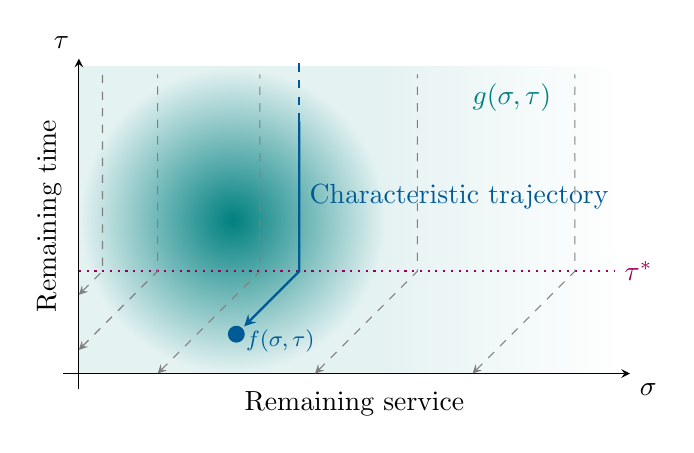
\begin{tikzpicture}
  
	\shade[inner color=teal,outer color=teal!10!white] (0,0) rectangle (3.9,3.9);
	\shade[left color=teal!10!white,right color=white] (3.9,0) rectangle (6.9,3.9);

  \node[teal] at (5.5,3.5) {$g(\sigma,\tau)$};
  \draw [->] (-.2,0) -- (7,0);
  \node [below right] at (7,0) {$\sigma$};
  \draw [->] (0,-.2) -- (0,4);
  \node [above left] at (0,4) {$\tau$};
  
  \node [below] at (3.5,-.1) {Remaining service};
  \node [rotate=90, left, anchor=south] at (-.1,2) {Remaining time};
  
%	\draw [thick,gray,->] (4,2.3) -- ++(0,-.4);
  \draw [rojito, dotted, thick] (0,1.3) -- (6.8,1.3) node[right] {$\tau^*$};
  \draw [azulcito, fill=azulcito] (2,.5) circle [radius=0.1] node[below right, yshift=5pt] {\footnotesize $f(\sigma,\tau)$};

  \draw [azulcito,thick,<-] (2.1,.6) -- (2.8,1.3) -- node[midway, anchor=west] {Characteristic trajectory} (2.8,3.2);
  \draw [azulcito,thick,dashed] (2.8,3.2) -- (2.8,4);

  \draw [gray,dashed,<-] (0,1) -- (.3,1.3) -- (.3,3.8);
  \draw [gray,dashed,<-] (0,.3) -- (1,1.3) -- (1,3.8);
  \draw [gray,dashed,<-] (1,0) -- (2.3,1.3) -- (2.3,3.8);
  \draw [gray,dashed,<-] (3,0) -- (4.3,1.3) -- (4.3,3.8);
  \draw [gray,dashed,<-] (5,0) -- (6.3,1.3) -- (6.3,3.8);

  \end{tikzpicture}
	\end{center}

\end{frame}

\begin{frame}{EDF in overload}{Fluid model equilibrium}

	\begin{theorem}
    Assume that $\rho > C$ and the equation
	\begin{equation*}
		\lambda E[\min\{S,T,\tau^*\}] = C
	\end{equation*}
    has a unique solution $\tau^* > 0$. Consider the measure $\mu^*$ given by the following density:
    \begin{equation*}
		f(\sigma, \tau) = \lambda\left[\int_0^{\left(\tau^* - \tau\right)^+} g(\sigma + u, \tau + u)du + \int_{\left(\tau^* - \tau\right)^+}^\infty g\left(\sigma + \left(\tau^* - \tau\right)^+, \tau + u\right)du\right]. 
	\end{equation*}

	This measure is a fluid equilibrium for the EDF policy, and 
	\begin{equation*}
	\tau^* = \sup \left\{\tau \geq 0:\mu^*(\R_{++} \times (0, \tau]) \leq C\right\}.
	\end{equation*}
	\end{theorem}

\end{frame}

\begin{frame}{EDF performance in equilibrium}
	
	\begin{columns}
		\begin{column}{0.5\textwidth}
		\begin{itemize}
		\item Let us compute the rate at which work is \alert{reneged}.
		
		\item Compute the rate at which mass exits with $S_r < \sigma_0$.
		
		\end{itemize}
		\end{column}
		\begin{column}{0.5\textwidth}
			\begin{tikzpicture}[scale=0.7]
				
			\draw [->] (-.2,0) -- (7,0);
			\node [below right] at (7,0) {$\sigma$};
			\draw [->] (0,-.2) -- (0,4);
			\node [above left] at (0,4) {$\tau$};
			
%			\node [below] at (3.5,-.1) {Remaining service};
%			\node [rotate=90, left, anchor=south] at (-.1,2) { Remaining time};

			\draw [gray, dotted, thick] (0,1.5) -- (6.8,1.5) node[black, right] {$\tau_\Phi$};

			\draw[very thick,rojito] (0,1.5) -- (0,0) -- (2,0);
			\draw[very thick,rojito] (2,.2) -- (2,-.2) node[below]{$\sigma_0$};

			\draw[thick,gray] (2,0) -- (3.5,1.5) -- (3.5,4);

			\draw[thick,gray,->] (1.75,3) -- ++(0,-.9);
			\draw[thick,gray,->] (1.5,1) -- ++(-.6,-.6);

			\end{tikzpicture}
		\end{column}
	\end{columns}

	\begin{proposition}
    \begin{equation*}
        \int_0^{\tau^*} f(0, \tau)d\tau + \int_0^{\sigma_0} f(\sigma, 0)d\sigma = \lambda P\left(S - \min\left\{S, T, \tau^*\right\} < \sigma_0\right).
    \end{equation*}

	\smallskip
	i.e. $S_a = S-S_r = \min\{S,T,\tau^*\}$.
	\end{proposition}
\end{frame}


\section{Deadline-oblivious policies}

\begin{frame}{What if we do not know the deadlines?}

	\begin{myitem}
	\item Deadlines are often hard to estimate in practice.
	\item Moreover, tasks may under-report their deadline to get priority!
	\item What about \alert{deadline-oblivious} policies?
	\begin{itemize}
		\item Can we model them?
		\item What is their performance?
	\end{itemize}
	\end{myitem}
	
	\pause
	\vfill
	\alert{Problem:} we need a new state-space...
\end{frame}


\begin{frame}{Attained service state descriptor}

	\begin{columns}
	\begin{column}{0.45\textwidth}
		  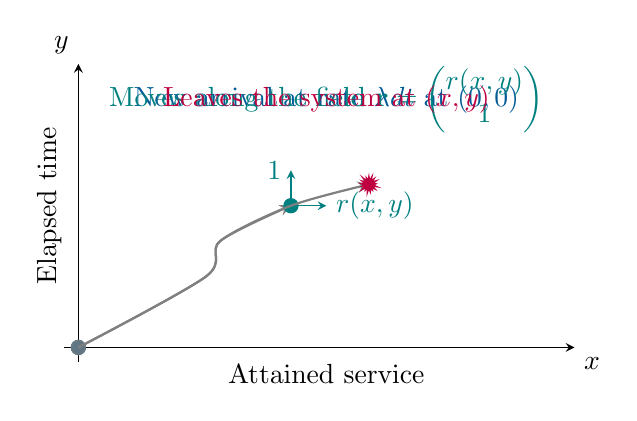
\begin{tikzpicture}[scale=0.9]
		
			\draw [->] (-.2,0) -- (7,0);
			\node [below right] at (7,0) {$x$};
			\draw [->] (0,-.2) -- (0,4);
			\node [above left] at (0,4) {$y$};
			
			\node [below] at (3.5,-.1) {Attained service};
			\node [rotate=90, left, anchor=south] at (-.1,2) {Elapsed time};

			\draw<2> [azulcito, fill=azulcito] (0,0) circle [radius=0.1];
			\node<2> [azulcito] at (3.5,3.5) {New arrival at rate $\lambda dt$ at $(0,0)$};

			\draw<3> [thick,gray,->] plot[smooth] coordinates {(0,0) (1.8,1) (2,1.5) (3,2)}; 
			\draw<3> [gray, fill=gray, opacity=0.5] (0,0) circle [radius=0.1];
			\draw<3> [teal, fill=teal] (3,2) circle [radius=0.1];
			\draw<3> [teal, fill=teal,->] (3,2) -- (3.5,2) node[right]{$r(x,y)$};
			\draw<3> [teal, fill=teal,->] (3,2) -- (3,2.5) node[left]{$1$};
			\node<3> [teal] at (3.5,3.5) {Moves along the field $\mathbf{r} = \begin{pmatrix}
			r(x,y) \\ 1
			\end{pmatrix}$};

			\draw<4-> [thick,gray,->] plot[smooth] coordinates {(0,0) (1.8,1) (2,1.5) (3,2) (4.1,2.3)}; 
			\draw<4-> [gray, fill=gray, opacity=0.5] (0,0) circle [radius=0.1];
			\node<4-> [purple, fill=purple, starburst, inner sep=1.5pt,/pgf/starburst point height=3] at (4.1,2.3) {};
			\node<4-> [purple] at (3.5,3.5) {Leaves the system at $(x,y)$};
			\end{tikzpicture}

	\end{column}
	\begin{column}{0.55\textwidth}
		\begin{itemize}
			\item<1-> Consider the elapsed time space.
			\item<3-> \alert{Policy} again defines how tasks are served.
			\item<3-> May depend on any combination of $(x,y)$.
			\item<5-> State descriptor:
			 \begin{equation*}
				\tilde\Phi_t = \sum_i \delta_{\left(x_i(t),y_i(t)\right)}
			 \end{equation*}
		\end{itemize}
	\end{column}
	\end{columns}

\end{frame}


\begin{frame}{Example: Least-Attained-Service policy}

	\begin{columns}
		\begin{column}{0.45\textwidth}
		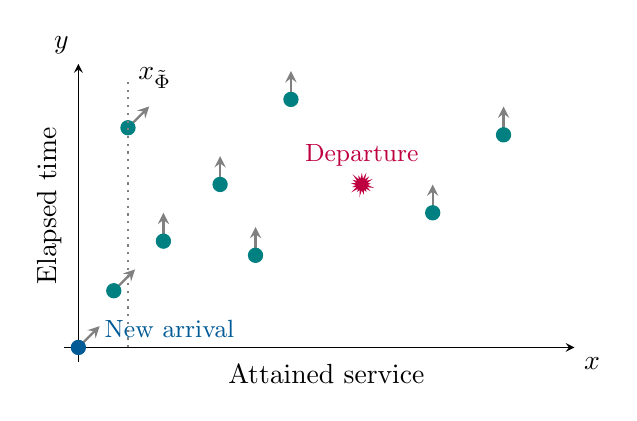
\begin{tikzpicture}[scale=0.9]
			\draw [->] (-.2,0) -- (7,0);
			\node [below right] at (7,0) {$x$};
			\draw [->] (0,-.2) -- (0,4);
			\node [above left] at (0,4) {$y$};
			
			\node [below] at (3.5,-.1) {Attained service};
			\node [rotate=90, left, anchor=south] at (-.1,2) {Elapsed time};
			
			\draw [thick,gray,->] (.5,.8) -- ++(.3,.3);
			\draw [thick,gray,->] (.7,3.1) -- ++(.3,.3);
			\draw [thick,gray,->] (1.2,1.5) -- ++(0,.4);
			\draw [thick,gray,->] (2,2.3) -- ++(0,.4);
			\draw [thick,gray,->] (2.5,1.3) -- ++(0,.4);
			\draw [thick,gray,->] (3,3.5) -- ++(0,.4);
			%\draw [thick,gray,->] (4,2.3) -- ++(.2,.4);
			\draw [thick,gray,->] (5,1.9) -- ++(0,.4);
			\draw [thick,gray,->] (6,3) -- ++(0,.4);

			\draw [teal, fill=teal] (.5,.8) circle [radius=0.1];
			\draw [teal, fill=teal] (.7,3.1) circle [radius=0.1];
			\draw [teal, fill=teal] (1.2,1.5) circle [radius=0.1];
			\draw [teal, fill=teal]  (2,2.3) circle [radius=0.1];
			\draw [teal, fill=teal] (2.5,1.3) circle [radius=0.1];
			\draw [teal, fill=teal] (3,3.5) circle [radius=0.1];
			%\draw [teal!50!white, fill=teal!50!white] (4,2.3) starburst  node[teal,above] {\footnotesize Departure};
			%\node[teal!50!white, fill=teal, starburst, inner sep=1.5pt,/pgf/starburst point height=3] at (4,2.3) {}; 
			%\node[teal,above, yshift=3pt] at (4,2.3) {\footnotesize Departure};
			
			\node[purple, fill=purple, starburst, inner sep=1.5pt,/pgf/starburst point height=3] at (4,2.3) {};
			\node[purple, above, yshift=3pt] at (4,2.3){ \small Departure};
			
			\draw [teal, fill=teal] (5,1.9) circle [radius=0.1];
			\draw [teal, fill=teal] (6,3) circle [radius=0.1];
			
			%new arrival

			\draw [thick,gray,->] (0,0) -- ++(.3,.3);
			\draw [azulcito, fill=azulcito] (0,0) circle [radius=0.1] node[anchor=south west, xshift=6pt] {\small New arrival};
			
			\draw [gray, dotted, thick] (.7,0) -- (.7,3.8) node[black, right] {$x_{\tilde{\Phi}}$};
	\end{tikzpicture}

	\end{column}
	\begin{column}{0.55\textwidth}
		\begin{itemize}
			\item Serve the $C$ least-served tasks.
			\item Corresponds to taking:
				\begin{equation*}
					r_{\tilde\Phi}(x,y) = \mathbf{1}_{\{x\leqslant x_{\tilde\Phi}\}} 
				\end{equation*}
				with
				\begin{equation*} 
					x_{\tilde\Phi} := \sup\{x: \tilde\Phi([0, x] \times \R_+) \leqslant C\}. 	
				\end{equation*} 
		\end{itemize}
	\end{column}
\end{columns}

\end{frame}


\begin{frame}{Example: Last-Come-First-Served policy}
  
	\begin{columns}
		\begin{column}{0.45\textwidth}
			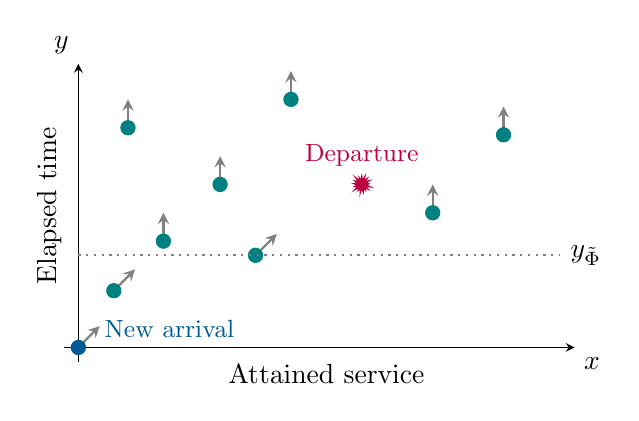
\begin{tikzpicture}[scale=0.9]
					
				\draw [->] (-.2,0) -- (7,0);
				\node [below right] at (7,0) {$x$};
				\draw [->] (0,-.2) -- (0,4);
				\node [above left] at (0,4) {$y$};
				
				\node [below] at (3.5,-.1) {Attained service};
				\node [rotate=90, left, anchor=south] at (-.1,2) {Elapsed time};
				
				\draw [thick,gray,->] (.5,.8) -- ++(.3,.3);
				\draw [thick,gray,->] (.7,3.1) -- ++(0,.4);
				\draw [thick,gray,->] (1.2,1.5) -- ++(0,.4);
				\draw [thick,gray,->] (2,2.3) -- ++(0,.4);
				\draw [thick,gray,->] (2.5,1.3) -- ++(.3,.3);
				\draw [thick,gray,->] (3,3.5) -- ++(0,.4);
				%\draw [thick,gray,->] (4,2.3) -- ++(.2,.4);
				\draw [thick,gray,->] (5,1.9) -- ++(0,.4);
				\draw [thick,gray,->] (6,3) -- ++(0,.4);

				\draw [teal, fill=teal] (.5,.8) circle [radius=0.1];
				\draw [teal, fill=teal] (.7,3.1) circle [radius=0.1];
				\draw [teal, fill=teal] (1.2,1.5) circle [radius=0.1];
				\draw [teal, fill=teal]  (2,2.3) circle [radius=0.1];
				\draw [teal, fill=teal] (2.5,1.3) circle [radius=0.1];
				\draw [teal, fill=teal] (3,3.5) circle [radius=0.1];
				%\draw [teal!50!white, fill=teal!50!white] (4,2.3) starburst  node[teal,above] {\footnotesize Departure};
				%\node[teal!50!white, fill=teal, starburst, inner sep=1.5pt,/pgf/starburst point height=3] at (4,2.3) {}; 
				%\node[teal,above, yshift=3pt] at (4,2.3) {\footnotesize Departure};
				\draw [teal, fill=teal] (5,1.9) circle [radius=0.1];
				\draw [teal, fill=teal] (6,3) circle [radius=0.1];
						
				\node[purple, fill=purple, starburst, inner sep=1.5pt,/pgf/starburst point height=3] at (4,2.3) {};
				\node[purple, above, yshift=3pt] at (4,2.3){ \small Departure};
				
				%new arrival

				\draw [thick,gray,->] (0,0) -- ++(.3,.3);
				\draw [azulcito, fill=azulcito] (0,0) circle [radius=0.1] node[anchor=south west, xshift=6pt] {\small New arrival};
				
				\draw [gray, dotted, thick] (0,1.3) -- (6.8,1.3) node[black, right] {$y_{\tilde{\Phi}}$};
				\end{tikzpicture}
		\end{column}
	\begin{column}{0.55\textwidth}
		\begin{itemize}
			\item Serve the $C$ more recent tasks.
			\item Corresponds to taking:
				\begin{equation*}
					r_{\tilde\Phi}(x,y) = \mathbf{1}_{\{y\leqslant y_{\tilde\Phi}\}} 
				\end{equation*}
				with
				\begin{equation*} 
					y_{\tilde\Phi} := \sup\{y: \tilde\Phi(\R_+\times [0, y]) \leqslant C\}
				\end{equation*} 
		\end{itemize}
	\end{column}
\end{columns}

\end{frame}

\begin{frame}{The hazard rate field}

	We have a new problem: what is the rate at which users \alert{leave} the system?

	\pause

	\vfill

	Let $\bar{G}(x,y) = P(S>x,T>y)$ and define:

	\begin{definition}[Hazard rate field]
		\begin{equation*}
			\mathbf{h}(x,y) = -\nabla \log \bar{G}(x,y)	\quad \text{i.e.}
		\end{equation*}
		\begin{itemize}
			\item $h^x (x,y) = P(S\in[x,x+dx],T>S \mid S>x,T>y)$
			\item $h^y (x,y) = P(T\in[y,y+dy],S>T \mid S>x,T>y)$
		\end{itemize}
	\end{definition}

	\vfill

	Interpretation: $\mathbf{h}$ stores the rate at which $\min\{S,T\}$ is attained due to $S$ or $T$ expiring.
\end{frame}

\begin{frame}{Fluid model dynamics}

	\begin{itemize}
		\item Replace $\tilde{\Phi}_t$ by a (fluid) measure $\nu_t$.
		\item Now mass arrives at $(0,0)$ at rate $\lambda$.
		\item Drifts along the field:
		 \begin{equation*}
			\mathbf{r}_\nu(x,y) = \begin{pmatrix}
				r_\nu (x,y) \\ 1
			\end{pmatrix}
		 \end{equation*}
		 \item With $r_\nu$ satisfying:
		 \begin{gather*}
			0\leqslant r_\nu \leqslant 1 \\
			\iint r_\nu(x,y) \nu(dx,dy) \leqslant \min\{\nu(\R^2_+),C\}.
		 \end{gather*}
	\end{itemize}
\end{frame}

% \begin{frame}{Departure rate}

% 	Now we have to compute the departure rate $\eta_{\nu}(x,y)$:
% 	\begin{equation*}
% 		\eta_\nu(x,y) := \lim_{dt\to 0} \frac{1}{dt} P\left(\left\{S\in\left(x,x+r_{\tilde\Phi}dt\right)\right\}\cup \left\{T\in\left(y,y+dt\right)\right\}\mid S>x,T>y\right)
% 	\end{equation*}

% 	By the chain rule and some computations:
% 	\begin{gather*}
% 		\eta_{\nu}(x,y) =\frac{1}{\bar{G}(x,y)}\left[-\frac{\partial}{\partial x} \bar{G}(x,y) r_{\tilde\Phi}(x,y) - \frac{\partial}{\partial y} \bar{G}(x,y)\right]
% 	\end{gather*}
% 	\pause
% 	Therefore:
% 	\begin{equation*}
% 	\eta_{\nu}(x,y) = h^x(x,y)r_{\nu}(x,y)+h^y(x,y) = \mathbf{r}_{\nu}(x,y) \cdot \mathbf{h}(x,y).
% 	\end{equation*}

% \end{frame}

\begin{frame}{Attained service transport equation}

	\begin{myitem}
		\item We now have all ingredients to formulate the dynamics of the system.
		\item The transport equation in the elapsed service space is (informally):
		\begin{equation*}
			\frac{\partial \bar f}{\partial t} + \nabla \cdot\left[\mathbf{r}_{\nu_t} \bar{f}\right] + [\mathbf{r}_{\nu_t}\cdot \mathbf{h}]\bar{f}= \lambda \delta_{(0,0)}.
		\end{equation*}
		where $\tilde{f}$ is the density of $\nu_t$.
		\pause
		\item The above equation must be treated in weak form:
		 \begin{itemize}
			\item To account for the impulse mass at $(0,0)$ driving the system.
			\item To allow solutions without a density as we shall see.
		 \end{itemize}
	\end{myitem}


\end{frame}


\begin{frame}{Last come first served}{Fluid equilibrium}

	Recall that LCFS can be modeled by:
	\begin{equation*}
		r_{\nu}(x, y) = \ind{y < y_\nu}
	\end{equation*}
	with
	\begin{equation*}
	y_\nu = \sup \left\{y \geq 0: \nu(\R_+ \times [0, y]) \leqslant C\right\}.
	\end{equation*}

	\pause
	\vfill
	Imposing equilibrium, $\nu^*$, $y^*$ fixed, we have to solve: 
	\begin{equation*}
		\nabla \cdot\left[\mathbf{r}_{\nu^*} \bar{f}\right] + [\mathbf{r}_{\nu^*}\cdot \mathbf{h}]\bar{f}= \lambda \delta_{(0,0)}.
	\end{equation*}

\end{frame}


\begin{frame}{Solving the transport equation}{Last come first served case}

	\begin{center}
	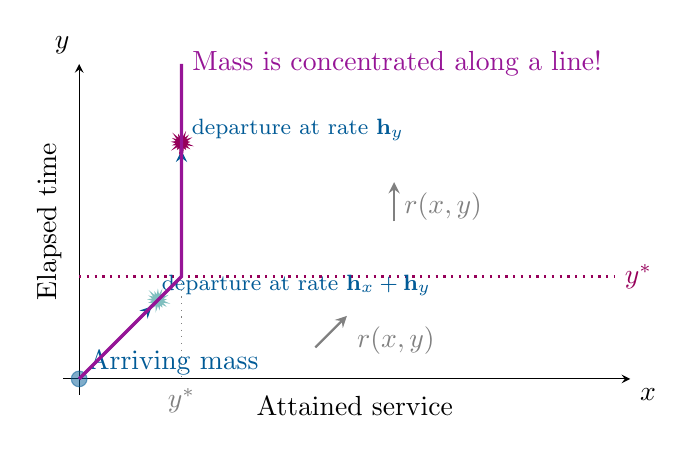
\begin{tikzpicture}
  
		\draw [->] (-.2,0) -- (7,0);
		\node [below right] at (7,0) {$x$};
		\draw [->] (0,-.2) -- (0,4);
		\node [above left] at (0,4) {$y$};
		
		\node [below] at (3.5,-.1) {Attained service};
		\node [rotate=90, left, anchor=south] at (-.1,2) {Elapsed time};

		\draw [gray,thick,->] (3,.4) -- (3.4,.8) node[below right] {$r(x,y)$};
		\draw [gray,thick, ->] (4,2) -- (4,2.5) node[below right] {$r(x,y)$};

		\draw [rojito, dotted, thick] (0,1.3) -- (6.8,1.3) node[right] {$y^*$};
		\draw [azulcito, fill=azulcito, opacity=0.5] (0,0) circle [radius=0.1]; 
		\node<1> [azulcito, anchor=west] at (0,.2) {Arriving mass};
		\draw<2> [azulcito,thick,->] (0,0) -- (.92,.92) node[above right] {\footnotesize departure at rate $\mathbf{h}_x+\mathbf{h}_y$};
		\node<2>[teal!50!white, fill=teal!50!white, starburst, inner sep=1.5pt,/pgf/starburst point height=3] at (1,1) {}; 
		\draw<3> [azulcito,thick,->] (0,0) -- (1.3,1.3) -- (1.3,2.9) node[above right] {\footnotesize departure at rate $\mathbf{h}_y$};
		\node<3>[rojito!50!white, fill=rojito, starburst, inner sep=1.5pt,/pgf/starburst point height=3] at (1.3,3) {}; 
		\draw<3>[gray, dotted] (1.3,1.3) -- (1.3,0) node[below] {$y^*$};

		\draw<4>[violetita, very thick] (0,0) -- (1.3,1.3) -- (1.3,4) node[right] {Mass is concentrated along a line!};
  \end{tikzpicture}

\end{center}

\end{frame}

\begin{frame}{Deadline-oblivious policies in overload}
	
	\begin{theorem}
    Assume that $\rho > C$ and the equation
	\begin{equation*}
		\lambda E[\min\{S,T,z^*\}] = C
	\end{equation*}
    has a unique solution $z^* > 0$. Consider the measure $\nu^*$ given by:
    \begin{equation*}
        \brackets{\phi}{\nu^*} = \lambda \left[\int_0^{z^*} \phi(u, u) \bar{G}(u, u)du + \int_{z^*}^\infty \phi\left(z^*, u\right)\bar{G}(z^*, u)du\right],
    \end{equation*}
    for all $\phi \in C_c(\R_+^2)$. Then this measure is the equilibrium measure for both the Least-Attained-Service and Last-Come-First-Served policies.
\end{theorem}

\end{frame}


\begin{frame}{LAS/LCFS performance in equilibrium}

	Compute the rate at which mass leaves the system with less than $x_0$ attained service:
	\begin{equation*}
		\iint_{[0,x_0]\times \R_+} \eta_{\nu^*} (x,y) \nu^*(dx,dy).
	\end{equation*}

	\pause

	\begin{proposition}
		Assume that $\rho > C$. Then
		\begin{equation*}
			\int_{[0,x_0]\times \R_+} \left[h^x(x, y) \ind{y < z^*} + h^y(x, y)\right]\nu^*(dx, dy) = \lambda P\left(\min\{S, T, z^*\} \leqslant x_0\right).
		\end{equation*}
	\end{proposition}
	
	So again the attained work is $S_a = \min\{S,T,z^*\}$!!

\end{frame}


\begin{frame}{Graphical explanation}

	\begin{center}
		
\tikzsetnextfilename{service_profile_edf}
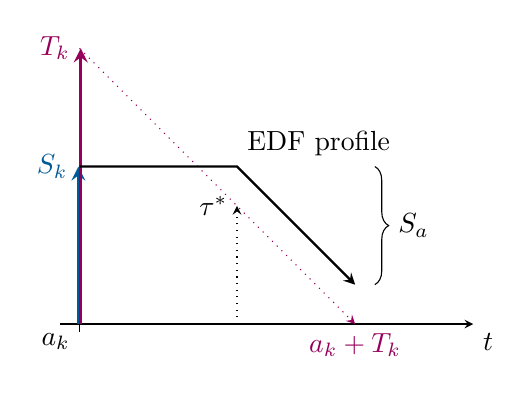
\begin{tikzpicture}[scale=0.5]
	\draw [->] (-.5,0) -- (10,0);
	\node [below right] at (10,0) {$t$};
	\draw [-] (0,-.2) -- (0,.2);
	\node [below left] at (0,0) {$a_k$};
	\draw [very thick,azulcito,->] (-.03,0) -- (-0.03,4) node  [left] {$S_k$};
	\draw [very thick,rojito,->] (.03,0) -- (0.03,7) node  [left] {$T_k$};
	\draw [dotted,rojito,->] (0,7) -- (7,0) node [below] {$a_k+T_k$};
	%\draw [dotted,azulcito,->] (0,4) -- (4,0) node [below] {$a_k+S_k$};
	%immediate scheduling
	\draw [black,thick,->] (0,4) -- (4,4) node[above right] {EDF profile}  -- (7,1);
	\draw [black,dotted,->] (4,0) -- (4,3) node [left] {$\tau^*$};

    \draw [decorate, decoration = {brace,mirror,amplitude=5pt}] (7.5,1) -- node[midway,right, xshift=5pt] {$S_a$} (7.5,4);

\end{tikzpicture}% \tikzsetnextfilename{service_profile_las_lcfs}
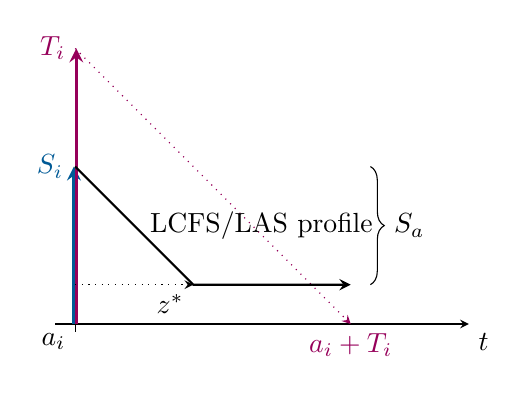
\begin{tikzpicture}[scale=0.5]
	
	\draw [->] (-.5,0) -- (10,0);
	\node [below right] at (10,0) {$t$};
	\draw [-] (0,-.2) -- (0,.2);
	\node [below left] at (0,0) {$a_i$};
	\draw [very thick,azulcito,->] (-.03,0) -- (-0.03,4) node  [left] {$S_i$};
	\draw [very thick,rojito,->] (.03,0) -- (0.03,7) node  [left] {$T_i$};
	\draw [dotted,rojito,->] (0,7) -- (7,0) node [below] {$a_i+T_i$};
	%\draw [dotted,azulcito,->] (0,4) -- (4,0) node [below] {$a_k+S_k$};
	%immediate scheduling
	\draw [black,thick,->] (0,4) -- node [midway, right,xshift=2pt] {LCFS/LAS profile} (3,1) -- (7,1);
	\draw [black,dotted,->] (0,1) -- (3,1) node [below left] {$z^*$};
	\draw [decorate, decoration = {brace,mirror,amplitude=5pt}] (7.5,1) -- node[midway,right, xshift=5pt] {$S_a$} (7.5,4);
\end{tikzpicture}%

	\end{center}

	\bigskip

	Since $\tau^* = x^* = y^* = z^*$, performance is the same in all three policies!!!
\end{frame}

\section{Simulations}

\begin{frame}{Simulations with correlated $S$ and $T$}
	\begin{itemize}
	\item We finally validate our fluid approximation by stochastic simulations
	\item In order to account for correlations, we take:
	 \begin{equation*}
    S = e^U \quad \text{and} \quad T = e^V \quad \text{with} \quad (U, V) \sim \mathcal{N}\left(\begin{pmatrix}
    0 \\ 0
    \end{pmatrix}, \begin{pmatrix}
    1 & 0.9 \\ 0.9 & 1
    \end{pmatrix}\right).
\end{equation*}
    \item In particular, the random variables $U$ and $V$ are correlated with normal distributions, and therefore $S$ and $T$ are correlated with log-normal distributions.
	\item In this case, $E[\min\{S,T\}] \approx 1.36$ can only be numerically estimated. 
	\item We choose $\lambda = 120$ and $C=100$, then $\rho\approx 160$ and $z^* \approx 1.322$.
	\end{itemize}
	

\end{frame}

\begin{frame}{State space snapshots}
    
	\begin{center}
	\only<1>{\tikzsetnextfilename{lognormal_edf_statespace}
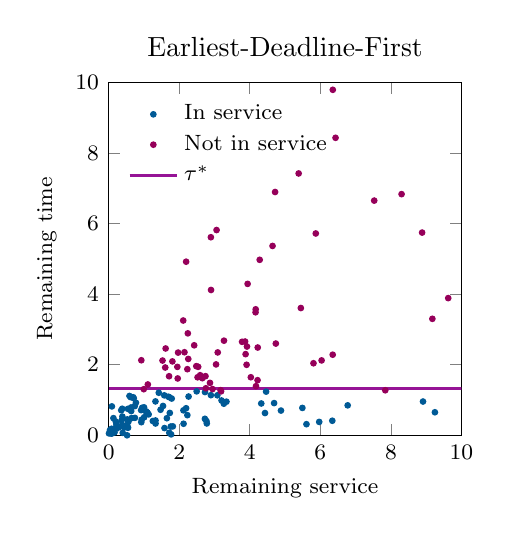
\begin{tikzpicture}

    \begin{axis}[
    title=Earliest-Deadline-First,
    width=0.5\textwidth,
    height=0.5\textwidth,
    xlabel={Remaining service},
    ylabel={Remaining time},
    xmin=0,xmax=10,
    ymin=0,ymax=10,
    legend style={font=\footnotesize},
    legend cell align=left,
    legend pos=north west,
    ]

    \addplot[color=azulcito, only marks, mark={*}, mark size=1.0 pt, mark options={color=azulcito, draw opacity={1.0}, fill=azulcito}]
        table[row sep={\\}]
        {
            \\
            42.02317704465638  0.5762050215730758  \\
            5.967868738242911  0.3805020986869485  \\
            9.246890979704283  0.653724251031818  \\
            12.788974453616916  0.36764266513799115  \\
            6.774920694569294  0.8497208802364042  \\
            4.325896008416223  0.9028994521191294  \\
            6.339212297130919  0.41381262035234756  \\
            1.582859536014058  0.20583406681080874  \\
            3.2002627968190325  0.9880748881351877  \\
            5.490845994551076  0.776927516996679  \\
            5.606908972317912  0.31590917793491347  \\
            2.4945438860528277  1.2462945694149568  \\
            4.88419873650348  0.701915776634479  \\
            4.462785801910971  1.2388767140834052  \\
            1.0968281481648754  0.6404263398894587  \\
            2.123865927986075  0.3287003945174405  \\
            3.2653051317376844  0.8968693426704135  \\
            8.909770443987584  0.9582366954198704  \\
            2.2313808357759886  0.5722159492392651  \\
            0.6500422838487152  0.48886313641490653  \\
            0.5507263116972039  0.21639387672010457  \\
            1.3306563525809016  0.3353242678256975  \\
            1.541504169695286  0.8323340956954159  \\
            1.2531589823126463  0.4061540805624164  \\
            1.7706033352684583  0.02715380739913087  \\
            0.3841629971131273  0.2902140639233579  \\
            2.727844337331778  0.4683676588917651  \\
            4.6898319829474975  0.9135968377258479  \\
            1.7185867793794074  0.07290371000667051  \\
            3.0817795791141958  1.1346616392071525  \\
            0.0508652177227327  0.05599085792707115  \\
            0.0872982006823988  0.04894743415658809  \\
            1.761883271021878  0.24979386844611895  \\
            0.9363352658182635  0.442432839271959  \\
            2.730938612086252  1.2260728170151083  \\
            2.781974022146266  0.33672122351643446  \\
            2.7721478800181636  0.40325229445295485  \\
            1.005403131051493  0.5120624616296825  \\
            1.6506098460879812  0.48567744131112556  \\
            0.7409798313125231  0.8281126318760816  \\
            3.339170600157008  0.9543019188921278  \\
            0.5289275541143763  0.4510719067027227  \\
            2.1956147480990484  0.768203713108548  \\
            1.0609100007632222  0.6817040484311434  \\
            4.431212377141655  0.6318414337582541  \\
            0.9260341914025099  0.37258485295848254  \\
            1.6899447510629488  1.0958820926567796  \\
            2.119310249133026  0.7077867913546498  \\
            0.6363215414620649  0.7902002795096621  \\
            1.8195527850391073  0.25383676676312916  \\
            1.003747939350164  0.7928813942612436  \\
            0.5227145813677694  0.0013151677457869937  \\
            1.1000177803193085  0.6451089066718085  \\
            0.44560008856757904  0.22484363230350368  \\
            0.6010779881494506  0.7307858131938048  \\
            0.36868123532034747  0.42492670517009423  \\
            1.3288976413578713  0.42121987985495957  \\
            1.0794229966881472  0.6352795025954949  \\
            0.08444223775010928  0.185972346302691  \\
            0.03783188633507284  0.14789602148316305  \\
            1.4209216493296402  1.2066826491852112  \\
            0.3846118305250217  0.7536645255955392  \\
            0.09220382128562798  0.8202814847106907  \\
            0.20329571489145715  0.3891088727454104  \\
            1.4714894037491217  0.7255690623465085  \\
            2.265918567835972  1.0994042509294104  \\
            0.13561553882915534  0.4874209195939869  \\
            0.15702578856275995  0.15758027446143785  \\
            0.38931758326869925  0.5318980162182783  \\
            0.3993570341066788  0.07005923456679852  \\
            0.009633129899231097  0.056118915935968516  \\
            2.8985692076163323  1.1386229791075806  \\
            0.22051885806506732  0.18934939853144783  \\
            0.22310800716737111  0.23390070919549544  \\
            1.1340123608900963  0.5939499127657797  \\
            0.22093417498307943  0.31673989251618195  \\
            1.3271883420990358  0.9616189569053546  \\
            0.621226491334065  1.083149442749047  \\
            0.3575239734389841  0.7102265169786364  \\
            1.7341969942113473  0.6344351424695134  \\
            0.29594807390969224  0.23085790562220154  \\
            1.7874515651307967  1.042600718852043  \\
            0.5395097964624036  0.21999031785647105  \\
            0.5910351679357635  1.1162789601212921  \\
            0.5176772999097088  0.29195116707577995  \\
            0.6941047891594229  1.0804921196055801  \\
            0.5605236170076723  0.3848519514552464  \\
            1.5770969033944655  1.1333063538832562  \\
            0.10230965039733131  0.0987746858295111  \\
            0.6399157550230428  0.6883771707435358  \\
            0.9205249018966153  0.7140826012965391  \\
            0.7445807145453807  0.4951346129180223  \\
            0.71273713691812  1.051291317362228  \\
            1.7276349425813584  1.077166754427239  \\
            0.5472134591030936  0.7505803511743636  \\
            0.1658887453101639  0.08266906167456511  \\
            0.9498650981656462  0.7807188920739634  \\
            0.2312037037768357  0.2651014381277861  \\
            0.773437348080346  0.9237406885496284  \\
            0.21349188453458362  0.229813303611067  \\
        }
        ;
    \addlegendentry {In service}

    \addplot[color=rojito, only marks, mark={*}, mark size=1.0 pt, mark options={color=rojito, draw opacity={1.0}, fill=rojito}]
        table[row sep={\\}]
        {
            \\
            25.981867809471318  5.0034946895449455  \\
            16.234193437663667  3.614895869657417  \\
            36.63760444624128  6.468753558531814  \\
            31.14528989401665  13.191811469568567  \\
            15.324583773995213  11.542442980796835  \\
            9.461014713387403  14.991017689239499  \\
            19.581733492574642  4.5377050585093865  \\
            3.8819164621819624  2.301196901117847  \\
            5.4476615951584275  3.6080294934613697  \\
            6.035823245650601  2.1237097081697103  \\
            21.6667512893535  4.902910743716841  \\
            9.623892021350908  3.889048403816931  \\
            12.25748424911653  3.8770119253427833  \\
            3.1730763947646623  1.2805512418388099  \\
            11.221124760384413  4.953231710799898  \\
            3.909626729620675  1.9995860018747198  \\
            4.176054211077368  1.3929523024633994  \\
            10.425323594992898  4.28924469277702  \\
            11.600908029079418  3.140791090637978  \\
            6.353570403087598  9.7923611438639  \\
            5.805769569970722  2.043217575600522  \\
            8.884347779212996  5.746414683679719  \\
            11.876911011169687  7.799013568018561  \\
            7.840111716267837  1.277059685045784  \\
            4.16760998372524  3.572215829418708  \\
            3.9389000155902947  4.292400464857675  \\
            9.278127618368273  11.62624057554067  \\
            3.187615945230718  1.247408574634008  \\
            3.8679652710215375  2.6582444470381414  \\
            4.030284982373518  1.6462131269032056  \\
            3.091969954711256  2.349597598778373  \\
            1.9474130730927355  1.9401799171823768  \\
            11.306517498671225  9.86133577292005  \\
            14.888599976017685  14.386839927522132  \\
            9.17496529696313  3.302340470353215  \\
            2.8975969861982804  5.614841310567808  \\
            5.870970502383145  5.72097396196072  \\
            21.339913463000588  6.656294501625579  \\
            2.7566332903337676  1.3340367139402076  \\
            3.0443506242681924  2.009980661148319  \\
            1.8070567214300033  2.095649526955526  \\
            4.163953099948308  3.487716910706866  \\
            2.231171953948759  1.8747359169356912  \\
            6.350767439811706  2.2852056343617733  \\
            2.5377833597693455  1.941856744503255  \\
            4.2202449497376175  1.5626340611924832  \\
            3.059261704795654  5.81836179378085  \\
            8.075545869602026  11.592105856727237  \\
            1.5273470278429744  2.1196962362141534  \\
            0.9266625792906856  2.1277322266382726  \\
            3.2688708652502965  2.683048854709355  \\
            5.385722001232905  7.421881487851367  \\
            2.1491614191750377  2.3550311440127984  \\
            3.7819414461100114  2.6501255998218056  \\
            3.920652637943882  2.516688659788713  \\
            9.150162390426537  14.23330433790592  \\
            1.713061351121705  1.6753267919154098  \\
            2.7451674243554045  1.6765841115158793  \\
            1.6044267129382115  1.9225270657739912  \\
            6.431125751981546  8.432150709657108  \\
            7.526956962283178  6.652732543195624  \\
            1.968514417968582  2.345206931727404  \\
            8.302332491101224  6.835943048710375  \\
            4.645739215506538  5.367897865744409  \\
            4.73840219461937  2.60104440453685  \\
            2.8723875642317296  1.4868883534750523  \\
            1.6156152913734865  2.4615920856206515  \\
            2.9439978948128003  1.3113889288031828  \\
            2.9024993109845076  4.119780938511253  \\
            2.6541342052361845  1.6194746652371919  \\
            2.520188608225367  1.6450601384413375  \\
            2.2567985039441316  2.165302328761385  \\
            10.016083167316307  7.829065099377685  \\
            4.717861427532198  6.896062943059318  \\
            4.225282878225343  2.4889000196047846  \\
            2.5927518802224325  1.7041743599559993  \\
            2.1960787997131628  4.921190192061998  \\
            15.17548353655256  11.248305329432256  \\
            1.1110092713879183  1.4415069689628979  \\
            2.4250384103178595  2.55161206518072  \\
            1.9575686906039376  1.6117966867635403  \\
            2.484600521802187  1.9608411555021945  \\
            2.113768735322044  3.254152364996102  \\
            2.2447245820377764  2.890521039812654  \\
            4.28157402260432  4.974768692204179  \\
            0.995880257636133  1.30764037540294  \\
        }
        ;
    \addlegendentry {Not in service}
    \addplot[color=violetita,solid, very thick]
        table[row sep={\\}]
        {
            \\
            0.0  1.322  \\
            20.0  1.322  \\
        }
        ;
    \addlegendentry {$\tau^*$}
\end{axis}
\end{tikzpicture}
}
    \only<2>{\tikzsetnextfilename{lognormal_las_statespace}
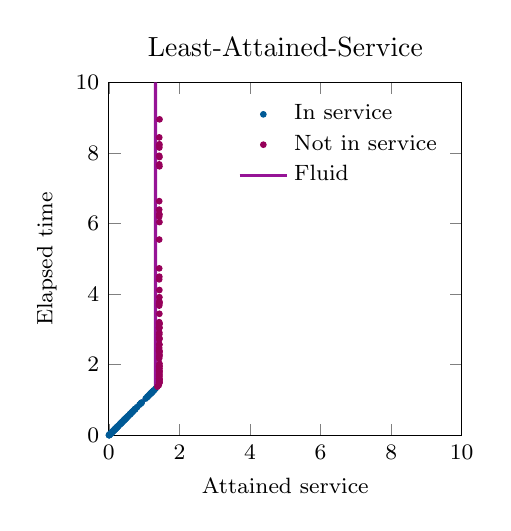
\begin{tikzpicture}

\begin{axis}[
    title=Least-Attained-Service,
    width=0.5\textwidth,
    height=0.5\textwidth,
    xlabel={Attained service},
    ylabel={Elapsed time},
    xmin=0,xmax=10,
    ymin=0,ymax=10,
    legend style={font=\footnotesize},
    legend cell align=left,
    legend pos=north east,
    ]
    \addplot[color=azulcito, only marks, mark={*}, mark size=1.0 pt, mark options={color=azulcito, draw opacity={1.0}, fill=azulcito}]
        table[row sep={\\}]
        {
            \\
            1.3212989716362318  1.3217754450760855  \\
            1.2738665620191516  1.2738665620191512  \\
            1.265701825598896  1.2657018255988959  \\
            1.240444661514589  1.2404446615145874  \\
            1.2185669814122093  1.2185669814122098  \\
            1.216070667728446  1.216070667728447  \\
            1.2042625660308062  1.2042625660308064  \\
            1.2014507987158543  1.2014507987158538  \\
            1.183391048854475  1.1833910488544745  \\
            1.1621119825081798  1.1621119825081792  \\
            1.1421754502235917  1.1421754502235917  \\
            1.1101255400356829  1.1101255400356824  \\
            1.092359905168678  1.0923599051686779  \\
            1.090353697670082  1.0903536976700825  \\
            1.0431440008927806  1.043144000892781  \\
            0.9277092201054133  0.9277092201054136  \\
            0.9215989559761795  0.9215989559761795  \\
            0.9040256052500126  0.9040256052500129  \\
            0.8701485196647809  0.8701485196647809  \\
            0.8005823732270875  0.8005823732270869  \\
            0.749540467085851  0.7495404670858508  \\
            0.7469240414121718  0.7469240414121714  \\
            0.746536441469404  0.7465364414694005  \\
            0.7278620595726721  0.7278620595726724  \\
            0.7035231510153328  0.7035231510153328  \\
            0.6813393060919566  0.6813393060919566  \\
            0.6719002134195331  0.6719002134195335  \\
            0.6530075665999959  0.6530075665999959  \\
            0.6456296752049031  0.6456296752049031  \\
            0.6224171952051736  0.6224171952051738  \\
            0.6108384411478767  0.6108384411478771  \\
            0.6039853202393749  0.6039853202393748  \\
            0.5931972381096391  0.5931972381096391  \\
            0.5912374032296699  0.5912374032296701  \\
            0.5877845625809789  0.5877845625809788  \\
            0.5501984748151761  0.550198474815176  \\
            0.5401083797634675  0.5401083797634674  \\
            0.5194383660455915  0.5194383660455917  \\
            0.509839879943442  0.5098398799434425  \\
            0.4953731406906181  0.495373140690619  \\
            0.49142823496197297  0.49142823496197297  \\
            0.4780769101721205  0.4780769101721205  \\
            0.46627731626586  0.46627731626586  \\
            0.46247116327809623  0.46247116327809623  \\
            0.4553250353014564  0.4553250353014562  \\
            0.443697758762284  0.4436977587622839  \\
            0.43299004407471386  0.43299004407471386  \\
            0.43172397448840627  0.43172397448840627  \\
            0.4219511592200438  0.4219511592200438  \\
            0.4113203670276988  0.4113203670276988  \\
            0.39907890324809614  0.3990789032480966  \\
            0.3745403787329453  0.3745403787329451  \\
            0.3733593625833862  0.37335936258338664  \\
            0.36489760069892396  0.36489760069892485  \\
            0.35664774400356736  0.35664774400356736  \\
            0.34895755711360765  0.34895755711360765  \\
            0.3469838491191415  0.3469838491191415  \\
            0.331058748422294  0.331058748422294  \\
            0.32926201698521096  0.3292620169852114  \\
            0.32500489792822407  0.3250048979282245  \\
            0.313042279379502  0.31304227937950246  \\
            0.28736571358770413  0.28736571358770435  \\
            0.2685361293347772  0.2685361293347772  \\
            0.2583450646898203  0.25834506468982044  \\
            0.24539186773515098  0.24539186773515098  \\
            0.24135147344719776  0.24135147344719599  \\
            0.2396467459062004  0.2396467459061995  \\
            0.23646590414111324  0.23646590414111346  \\
            0.21868085918322366  0.21868085918322366  \\
            0.21641195542163416  0.21641195542163416  \\
            0.20883054507197585  0.2088305450719763  \\
            0.20253059717936162  0.20253059717936184  \\
            0.19556066286878648  0.19556066286878648  \\
            0.1842788538808544  0.18427885388085485  \\
            0.18227365438312448  0.18227365438312448  \\
            0.1725793438215394  0.1725793438215395  \\
            0.1667127240394315  0.16671272403942972  \\
            0.16115736269021896  0.16115736269021896  \\
            0.15920368125134177  0.15920368125134177  \\
            0.1448802609186406  0.1448802609186406  \\
            0.1389996771241897  0.1389996771241897  \\
            0.12900219730472928  0.12900219730472928  \\
            0.11782043267611231  0.11782043267611231  \\
            0.11587847115491501  0.11587847115491501  \\
            0.09326639660011482  0.09326639660011438  \\
            0.08426623937559485  0.08426623937559441  \\
            0.07869445685192078  0.07869445685192078  \\
            0.07651580596446106  0.07651580596446195  \\
            0.06705748724594729  0.06705748724594729  \\
            0.059744694970874423  0.059744694970874423  \\
            0.059620721306317126  0.059620721306317126  \\
            0.05073908005324812  0.05073908005324812  \\
            0.03724433090836543  0.03724433090836543  \\
            0.029189103467743838  0.029189103467743838  \\
            0.021481493445037803  0.021481493445037803  \\
            0.016404859937424465  0.016404859937424465  \\
            0.011551930358522089  0.011551930358522089  \\
            0.00934026486636741  0.00934026486636741  \\
            0.005373022076725409  0.005373022076725409  \\
            0.004687414766195719  0.004687414766195719  \\
        }
        ;
    \addlegendentry {In service}

    \addplot[color=rojito, only marks, mark={*}, mark size=1.0 pt, mark options={color=rojito, draw opacity={1.0}, fill=rojito}]
        table[row sep={\\}]
        {
            \\
            1.4280901432422937  36.39104916050235  \\
            1.431521389781146  16.953475822197273  \\
            1.430810114063915  13.89502240307612  \\
            1.4316124185148382  11.150240979042767  \\
            1.4324709431377727  10.468110179898273  \\
            1.4274756267350988  10.375658504853666  \\
            1.435576020348213  8.955621438192145  \\
            1.4278972457203354  8.444290711119582  \\
            1.4324704553646939  8.249246062087371  \\
            1.4260748369731484  8.20590925685861  \\
            1.4302647267972688  8.156671351732443  \\
            1.4262827344146505  7.923402073466123  \\
            1.4334291299763677  7.886180600256498  \\
            1.4279454577309236  7.679335506474859  \\
            1.43367972574152  7.624280914868468  \\
            1.4272267675675874  6.637320355073671  \\
            1.4260893487210495  6.396648650750949  \\
            1.4308372269241922  6.264605973545129  \\
            1.4302032019344137  6.252343456809541  \\
            1.4260630034700732  6.196235378304625  \\
            1.4334167475816364  6.043317267008009  \\
            1.426089648216038  5.548401378617216  \\
            1.426009820488515  4.732498462097141  \\
            1.4302559547102085  4.4975153116355955  \\
            1.4260095072521164  4.421412223598392  \\
            1.4312845075646807  4.118318400680634  \\
            1.4324258868550148  3.9153587878485046  \\
            1.4311480637430285  3.7936020194811837  \\
            1.4337523553359661  3.766736354032574  \\
            1.4262267575541  3.739153793609234  \\
            1.4262030736907931  3.7168698338789614  \\
            1.4262161017294286  3.6763136759010724  \\
            1.4306117364263793  3.4453304760317263  \\
            1.4264480464957252  3.2063050900217434  \\
            1.4272253764365042  3.188322139688152  \\
            1.4279605234057153  3.171496359792471  \\
            1.4305276995383962  3.15511716207044  \\
            1.4312867377323464  3.1535792586801383  \\
            1.4285440348269987  3.0629599973318857  \\
            1.4260914304963306  3.055032775075005  \\
            1.4282662715822605  3.045939359024458  \\
            1.4264508994622918  3.034372059699037  \\
            1.4315825948953784  2.910380566689994  \\
            1.427308932946909  2.857951619865986  \\
            1.4262819322893232  2.7646422263821075  \\
            1.4337502017647177  2.745087013196538  \\
            1.4298028711012867  2.719879122520992  \\
            1.4272183905934401  2.5759153255365863  \\
            1.433696657095232  2.572310769446161  \\
            1.426231089520135  2.4758468986710227  \\
            1.4262672006216164  2.409407151132543  \\
            1.4260646249605866  2.39827712351539  \\
            1.4316135826455718  2.375879896679876  \\
            1.427221929569098  2.375631939979086  \\
            1.4311763175186978  2.344928291844668  \\
            1.4355275544176846  2.276711259110356  \\
            1.430256195245911  2.2344858114254005  \\
            1.4263840835790125  2.1830603463430975  \\
            1.4355222999217678  2.0277895813573257  \\
            1.4315916601751821  1.9649181390778523  \\
            1.4308349209303024  1.9570683548150787  \\
            1.4262648855021833  1.9449785441188734  \\
            1.4336803338285788  1.8977922432147238  \\
            1.426038692759775  1.839218995346258  \\
            1.4309965753777085  1.8367832017842485  \\
            1.4272662015254978  1.8132006420502482  \\
            1.431127865762406  1.8032618656846755  \\
            1.4315320945174645  1.7688919043769575  \\
            1.4279602983602349  1.7337141275842214  \\
            1.4280860681276693  1.7108845574980904  \\
            1.4260845955983676  1.706528836552609  \\
            1.4302637820744901  1.66334685915453  \\
            1.426301703124155  1.6617725927769005  \\
            1.426332540730697  1.6130227463236653  \\
            1.4263421074384333  1.6068975755901391  \\
            1.4306112168432596  1.5855852297378166  \\
            1.4336929020922606  1.580941926297939  \\
            1.430959031032586  1.5503903168065278  \\
            1.4309867960642462  1.5276687314372737  \\
            1.4266111547034934  1.5126459594530532  \\
            1.4293848922864498  1.4964423795323967  \\
            1.4284653808721965  1.4882100758430719  \\
            1.430207243275078  1.4824251880297084  \\
            1.4142670249068345  1.4236072897732015  \\
            1.3753859621053264  1.3807589841820518  \\
        }
        ;
    \addlegendentry {Not in service}
    \addplot[color=violetita,solid, very thick]
        table[row sep={\\}]
        {
            \\
            0.0  0.0  \\
            1.322  1.322  \\
            1.322  10.0  \\
        }
        ;
    \addlegendentry {Fluid}
\end{axis}
\end{tikzpicture}
}
    \only<3>{\tikzsetnextfilename{lognormal_lcfs_statespace}
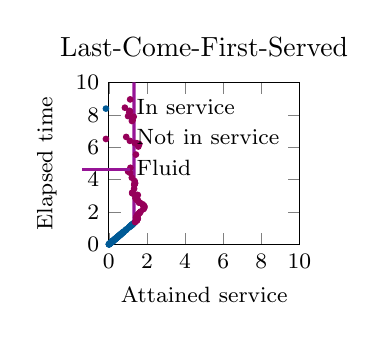
\begin{tikzpicture}
    \begin{axis}[
     title=Last-Come-First-Served,
    width=0.33\textwidth,
    height=0.3\textwidth,
    xlabel={Attained service},
    ylabel={Elapsed time},
    xmin=0,xmax=10,
    ymin=0,ymax=10,
    legend style={font=\footnotesize},
    legend cell align=left,
    legend pos=north east,
    ]

    \addplot[color=azulcito, only marks, mark={*}, mark size=1.0 pt, mark options={color=azulcito, draw opacity={1.0}, fill=azulcito}]
        table[row sep={\\}]
        {
            \\
            1.3212989716362473  1.3217754450761006  \\
            1.2738665620191658  1.2738665620191658  \\
            1.2657018255989105  1.2657018255989105  \\
            1.2404446615145996  1.2404446615146019  \\
            1.2185669814122218  1.218566981412224  \\
            1.2160706677284603  1.2160706677284576  \\
            1.2042625660308208  1.2042625660308208  \\
            1.201450798715869  1.2014507987158685  \\
            1.1833910488544892  1.1833910488544892  \\
            1.162111982508194  1.1621119825081938  \\
            1.1421754502236023  1.1421754502236094  \\
            1.110125540035697  1.1101255400356966  \\
            1.0923599051686925  1.0923599051686925  \\
            1.0903536976700965  1.0903536976700967  \\
            1.0431440008927952  1.0431440008927955  \\
            0.9277092201054278  0.9277092201054278  \\
            0.9215989559761939  0.9215989559761941  \\
            0.9040256052500271  0.9040256052500273  \\
            0.8701485196647956  0.8701485196647951  \\
            0.8005823732271017  0.8005823732271011  \\
            0.7495404670858514  0.749540467085851  \\
            0.7469240414121718  0.7469240414121714  \\
            0.7465364414694022  0.7465364414694022  \\
            0.7278620595726726  0.7278620595726726  \\
            0.7035231510153328  0.7035231510153328  \\
            0.6813393060919566  0.6813393060919566  \\
            0.6719002134195331  0.6719002134195335  \\
            0.6530075665999817  0.6530075665999817  \\
            0.6456296752048889  0.6456296752048889  \\
            0.6224171952051594  0.6224171952051596  \\
            0.6108384411478625  0.6108384411478629  \\
            0.6039853202393607  0.6039853202393606  \\
            0.5931972381096249  0.5931972381096249  \\
            0.5912374032296557  0.5912374032296559  \\
            0.5877845625809647  0.5877845625809646  \\
            0.5501984748151619  0.5501984748151618  \\
            0.5401083797634533  0.5401083797634532  \\
            0.5194383660455772  0.5194383660455775  \\
            0.5098398799434278  0.5098398799434283  \\
            0.4953731406906039  0.4953731406906048  \\
            0.49142823496195875  0.49142823496195875  \\
            0.4780769101721063  0.4780769101721063  \\
            0.4662773162658458  0.4662773162658458  \\
            0.462471163278082  0.462471163278082  \\
            0.4553250353014422  0.45532503530144197  \\
            0.4436977587622698  0.4436977587622697  \\
            0.43299004407469965  0.43299004407469965  \\
            0.43172397448839206  0.43172397448839206  \\
            0.42195115922002957  0.42195115922002957  \\
            0.4113203670276846  0.4113203670276846  \\
            0.39907890324808193  0.3990789032480824  \\
            0.3745403787329311  0.3745403787329309  \\
            0.3733593625833862  0.37335936258338664  \\
            0.36489760069892396  0.36489760069892485  \\
            0.35664774400356736  0.35664774400356736  \\
            0.34895755711360765  0.34895755711360765  \\
            0.3469838491191415  0.3469838491191415  \\
            0.331058748422294  0.331058748422294  \\
            0.32926201698521096  0.3292620169852114  \\
            0.32500489792822407  0.3250048979282245  \\
            0.313042279379502  0.31304227937950246  \\
            0.28736571358770413  0.28736571358770435  \\
            0.2685361293347772  0.2685361293347772  \\
            0.2583450646898203  0.25834506468982044  \\
            0.24539186773515098  0.24539186773515098  \\
            0.24135147344719776  0.24135147344719599  \\
            0.2396467459062004  0.2396467459061995  \\
            0.23646590414111324  0.23646590414111346  \\
            0.21868085918322366  0.21868085918322366  \\
            0.21641195542163416  0.21641195542163416  \\
            0.20883054507197585  0.2088305450719763  \\
            0.20253059717936162  0.20253059717936184  \\
            0.19556066286878648  0.19556066286878648  \\
            0.1842788538808544  0.18427885388085485  \\
            0.18227365438312448  0.18227365438312448  \\
            0.1725793438215394  0.1725793438215395  \\
            0.1667127240394315  0.16671272403942972  \\
            0.16115736269021896  0.16115736269021896  \\
            0.15920368125134177  0.15920368125134177  \\
            0.1448802609186406  0.1448802609186406  \\
            0.1389996771241897  0.1389996771241897  \\
            0.12900219730472928  0.12900219730472928  \\
            0.11782043267611231  0.11782043267611231  \\
            0.11587847115491501  0.11587847115491501  \\
            0.09326639660011482  0.09326639660011438  \\
            0.08426623937559485  0.08426623937559441  \\
            0.07869445685192078  0.07869445685192078  \\
            0.07651580596446106  0.07651580596446195  \\
            0.06705748724594729  0.06705748724594729  \\
            0.059744694970874423  0.059744694970874423  \\
            0.059620721306317126  0.059620721306317126  \\
            0.05073908005324812  0.05073908005324812  \\
            0.03724433090836543  0.03724433090836543  \\
            0.029189103467743838  0.029189103467743838  \\
            0.021481493445037803  0.021481493445037803  \\
            0.016404859937424465  0.016404859937424465  \\
            0.011551930358522089  0.011551930358522089  \\
            0.00934026486636741  0.00934026486636741  \\
            0.005373022076725409  0.005373022076725409  \\
            0.004687414766195719  0.004687414766195719  \\
        }
        ;
    \addlegendentry {In service}

    \addplot[color=rojito, only marks, mark={*}, mark size=1.0 pt, mark options={color=rojito, draw opacity={1.0}, fill=rojito}]
        table[row sep={\\}]
        {
            \\
            1.5339057821053927  36.39104916050237  \\
            1.1745894454722219  16.953475822197262  \\
            1.0124216387545424  13.895022403076178  \\
            1.1529475178358126  11.15024097904283  \\
            1.9102757805727428  10.468110179898398  \\
            1.851288258037533  10.375658504853769  \\
            1.116387458958755  8.955621438192237  \\
            0.8402804030534554  8.444290711119637  \\
            1.0830474907394922  8.249246062087426  \\
            1.115313132418577  8.205909256858664  \\
            1.07051522812867  8.156671351732498  \\
            1.0072892234652642  7.92340207346618  \\
            1.3039496123640166  7.886180600256557  \\
            1.2458598001686605  7.679335506474915  \\
            1.2076606527297287  7.624280914868526  \\
            0.9090249412707028  6.637320355073724  \\
            1.1031576813748885  6.396648650750988  \\
            1.35625285488412  6.264605973545157  \\
            1.468550262574249  6.2523434568095695  \\
            1.5965126264249285  6.196235378304637  \\
            1.5459432297243727  6.043317267008033  \\
            1.4192505274158123  5.548401378617241  \\
            1.1302462628480878  4.7324984620971655  \\
            1.0093782701179332  4.497515311635622  \\
            1.1134241402242209  4.42141222359842  \\
            1.2056543392212795  4.118318400680648  \\
            1.3514438865231464  3.9153587878485188  \\
            1.371580189465556  3.7936020194811975  \\
            1.3654255803936204  3.7667363540325876  \\
            1.3632738969293685  3.739153793609248  \\
            1.3427569537849315  3.716869833878972  \\
            1.3312087320619552  3.676313675901084  \\
            1.3247591624570005  3.44533047603174  \\
            1.2340629640692216  3.2063050900217585  \\
            1.23158023080273  3.1883221396881676  \\
            1.224024407792909  3.1714963597924712  \\
            1.2390449722392016  3.15511716207044  \\
            1.26028173782621  3.1535792586801397  \\
            1.406443183188907  3.062959997331882  \\
            1.4905554518697404  3.055032775075006  \\
            1.5189501527724043  3.0459393590244583  \\
            1.4243644598152656  2.910380566689994  \\
            1.3975499545286922  2.8579516198659825  \\
            1.4397399403273998  2.7646422263821075  \\
            1.5031048402365785  2.7450870131965392  \\
            1.5243209721578501  2.7198791225209935  \\
            1.5837179983719611  2.5759153255365863  \\
            1.6351587579007676  2.5723107694461613  \\
            1.7753087963413332  2.4758468986710227  \\
            1.807111416170355  2.409407151132543  \\
            1.809239581673804  2.39827712351539  \\
            1.8534066829538116  2.3756319399790873  \\
            1.858128381592941  2.3449282918446706  \\
            1.8618053388592415  2.2767112591103564  \\
            1.839676597792268  2.2344858114254014  \\
            1.8172764251526279  2.1830603463431  \\
            1.667286928120614  2.0277895813573266  \\
            1.615960581964246  1.9649181390778536  \\
            1.6162973651248227  1.9570683548150787  \\
            1.6139197956965763  1.9449785441188734  \\
            1.5685302262295133  1.8977922432147252  \\
            1.5202844118152807  1.8367832017842485  \\
            1.4933885429416178  1.8032618656846755  \\
            1.4851140682718524  1.7688919043769578  \\
            1.4879013192296195  1.7337141275842214  \\
            1.4662792710219184  1.7108845574980918  \\
            1.4651773631054121  1.7065288365526072  \\
            1.4291213494751571  1.66334685915453  \\
            1.4607913098878331  1.6617725927768987  \\
            1.4751387028166683  1.6130227463236655  \\
            1.5160456126054243  1.6068975755901374  \\
            1.506890772885896  1.5855852297378168  \\
            1.504426120333478  1.5809419262979403  \\
            1.4833328295605819  1.5503903168065287  \\
            1.4679240364663995  1.5276687314372746  \\
            1.454504102848106  1.5126459594530535  \\
            1.4597850653196796  1.496442379532395  \\
            1.4699120016327165  1.4882100758430727  \\
            1.470873257671188  1.4824251880297097  \\
            1.4142670249068328  1.4236072897732024  \\
            1.3753859621053122  1.3807589841820378  \\
        }
        ;
    \addlegendentry {Not in service}
    \addplot[color=violetita,solid, very thick]
        table[row sep={\\}]
        {
            \\
            0.0  0.0  \\
            1.322  1.322  \\
            1.322  10.0  \\
        }
        ;
    \addlegendentry {Fluid}
\end{axis}
\end{tikzpicture}
}
    \end{center}

	\vfill
	Blue dots are in service, red dots are not in service. 
\end{frame}

% \begin{frame}{Stochastic threshold evolution}
% 	\begin{center}
% 	\tikzsetnextfilename{lognormal_edf_threshold}
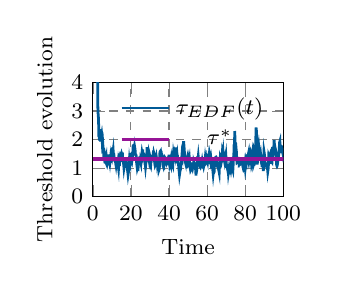
\begin{tikzpicture}
    \begin{axis}[
    %title=Earliest-Deadline-First,
    width=0.33\textwidth,
    height=0.25\textwidth,
    xlabel={Time},
    ylabel={Threshold evolution},
    ymin=0,ymax=4,
    xmin=0,xmax=100,
    grid,
    legend pos=north east,
    ]
    \addplot[color=azulcito, solid, line width=1pt]
        table[row sep={\\}]
        {
            \\
            1.8333333333333333  6.6540626551108595  \\
            2.0  4.734149204075039  \\
            2.1666666666666665  5.906793395299735  \\
            2.3333333333333335  5.264309124111591  \\
            2.5  4.212973247576047  \\
            2.6666666666666665  3.064447619811961  \\
            2.8333333333333335  2.847986058882015  \\
            3.0  2.7311142864786273  \\
            3.1666666666666665  2.125944655620207  \\
            3.3333333333333335  2.1145609426368535  \\
            3.5  1.968079872369151  \\
            3.6666666666666665  2.286202864818986  \\
            3.8333333333333335  2.2778250127348127  \\
            4.0  1.9327327457688526  \\
            4.166666666666667  2.368076631899966  \\
            4.333333333333333  2.007910041624479  \\
            4.5  2.133332900623319  \\
            4.666666666666667  2.1902258624804904  \\
            4.833333333333333  2.083311352630389  \\
            5.0  1.8694029126744205  \\
            5.166666666666667  1.9218842259368918  \\
            5.333333333333333  1.757825261556376  \\
            5.5  1.6456249872944797  \\
            5.666666666666667  1.5278568872004523  \\
            5.833333333333333  1.369934804288396  \\
            6.0  1.5403030017669275  \\
            6.166666666666667  1.3669469093995588  \\
            6.333333333333333  1.2052829627849695  \\
            6.5  1.200968774007522  \\
            6.666666666666667  1.3636141366064063  \\
            6.833333333333333  1.309767832298907  \\
            7.0  1.3647913474755553  \\
            7.166666666666667  1.152206723929262  \\
            7.333333333333333  1.1242043416784195  \\
            7.5  1.200366771394271  \\
            7.666666666666667  1.2040225355228678  \\
            7.833333333333333  1.3404156025646625  \\
            8.0  1.335577897502719  \\
            8.166666666666666  1.3111480983031414  \\
            8.333333333333334  1.2689841673875981  \\
            8.5  1.4794857433126438  \\
            8.666666666666666  1.2939247948040622  \\
            8.833333333333334  1.2972251925294245  \\
            9.0  1.214029363708427  \\
            9.166666666666666  1.3074524658560387  \\
            9.333333333333334  1.177208246020638  \\
            9.5  1.294238699052193  \\
            9.666666666666666  1.3378568577164174  \\
            9.833333333333334  1.5032192051875057  \\
            10.0  1.3139631321692011  \\
            10.166666666666666  1.5693814437466287  \\
            10.333333333333334  1.723741774997487  \\
            10.5  1.5570751083308174  \\
            10.666666666666666  1.629352036091357  \\
            10.833333333333334  1.4477465259858153  \\
            11.0  1.5337068122725444  \\
            11.166666666666666  1.3363785240922263  \\
            11.333333333333334  1.338364166480503  \\
            11.5  1.2599611525124956  \\
            11.666666666666666  1.252118829061832  \\
            11.833333333333334  1.2593461453995056  \\
            12.0  1.171102077712396  \\
            12.166666666666666  1.1036656314958426  \\
            12.333333333333334  1.194069334653149  \\
            12.5  1.249721319883827  \\
            12.666666666666666  1.3430795279083299  \\
            12.833333333333334  1.0914765552283787  \\
            13.0  1.09437301611189  \\
            13.166666666666666  1.1798866072491978  \\
            13.333333333333334  1.072930975748804  \\
            13.5  0.9915021007468536  \\
            13.666666666666666  1.1552951198959347  \\
            13.833333333333334  1.1504513202583793  \\
            14.0  1.1457938927502689  \\
            14.166666666666666  1.314383973755456  \\
            14.333333333333334  1.5133090437538015  \\
            14.5  1.3384642821302228  \\
            14.666666666666666  1.573793490513875  \\
            14.833333333333334  1.4689110162859293  \\
            15.0  1.4333950205747712  \\
            15.166666666666666  1.4932748936671327  \\
            15.333333333333334  1.457569499347161  \\
            15.5  1.5479049820248254  \\
            15.666666666666666  1.2974693788610216  \\
            15.833333333333334  1.3059407773027534  \\
            16.0  1.2532518156959018  \\
            16.166666666666668  1.1364390261009625  \\
            16.333333333333332  1.0161211297725674  \\
            16.5  1.0965173772235266  \\
            16.666666666666668  1.2048253010056857  \\
            16.833333333333332  1.3566893185597988  \\
            17.0  1.259625468626659  \\
            17.166666666666668  1.2232384996876147  \\
            17.333333333333332  1.1721399998112365  \\
            17.5  1.133240578101454  \\
            17.666666666666668  1.1433983782027752  \\
            17.833333333333332  1.0645039238818692  \\
            18.0  1.0160207730150341  \\
            18.166666666666668  0.921400147249372  \\
            18.333333333333332  0.8838399743485814  \\
            18.5  0.7766380093246923  \\
            18.666666666666668  0.8494722525713634  \\
            18.833333333333332  0.9600144633393732  \\
            19.0  1.1372653927536973  \\
            19.166666666666668  1.2747201612107855  \\
            19.333333333333332  1.1936796245113683  \\
            19.5  1.1545020307259115  \\
            19.666666666666668  1.44096925375287  \\
            19.833333333333332  1.455920859632094  \\
            20.0  1.291284769535348  \\
            20.166666666666668  1.1494957760953826  \\
            20.333333333333332  1.2737762514471935  \\
            20.5  1.2388065990434427  \\
            20.666666666666668  1.3203161587884762  \\
            20.833333333333332  1.4517776962416242  \\
            21.0  1.5324366029332257  \\
            21.166666666666668  1.7861365590554463  \\
            21.333333333333332  1.793305706618479  \\
            21.5  1.5612729545559247  \\
            21.666666666666668  1.5439380850121522  \\
            21.833333333333332  1.5905755778613133  \\
            22.0  1.7254463250859677  \\
            22.166666666666668  1.6613733845676713  \\
            22.333333333333332  1.4982145203488242  \\
            22.5  1.4770839902278383  \\
            22.666666666666668  1.460067187251887  \\
            22.833333333333332  1.4098394755032295  \\
            23.0  1.1803217062491451  \\
            23.166666666666668  1.0810006476586573  \\
            23.333333333333332  0.989632337699084  \\
            23.5  1.0300480871395408  \\
            23.666666666666668  0.8991970817498292  \\
            23.833333333333332  1.0461655480088372  \\
            24.0  1.2235938193547549  \\
            24.166666666666668  1.1053944529685644  \\
            24.333333333333332  1.2499672996613542  \\
            24.5  1.3231186030287505  \\
            24.666666666666668  1.4040628324124036  \\
            24.833333333333332  1.105916419643001  \\
            25.0  1.2439166751115556  \\
            25.166666666666668  1.1945308750851673  \\
            25.333333333333332  1.4425059985668334  \\
            25.5  1.3240259007983655  \\
            25.666666666666668  1.4399025047881757  \\
            25.833333333333332  1.543904531493796  \\
            26.0  1.4885682138910887  \\
            26.166666666666668  1.6504728359653882  \\
            26.333333333333332  1.4805817310566454  \\
            26.5  1.3600386650778207  \\
            26.666666666666668  1.3796588953402522  \\
            26.833333333333332  1.3973037117823677  \\
            27.0  1.2986717798047431  \\
            27.166666666666668  1.2821944214855598  \\
            27.333333333333332  1.2647355368329691  \\
            27.5  1.1700106187440262  \\
            27.666666666666668  1.0573292443540185  \\
            27.833333333333332  1.1563866221773544  \\
            28.0  1.2960857115771305  \\
            28.166666666666668  1.4420714971695787  \\
            28.333333333333332  1.4718238602557925  \\
            28.5  1.734972936318016  \\
            28.666666666666668  1.5683062696513446  \\
            28.833333333333332  1.524787181711515  \\
            29.0  1.4323653307486388  \\
            29.166666666666668  1.4683561598227932  \\
            29.333333333333332  1.3912538230177875  \\
            29.5  1.5485511889348254  \\
            29.666666666666668  1.5051179453098609  \\
            29.833333333333332  1.434808619026953  \\
            30.0  1.3110859729359612  \\
            30.166666666666668  1.101475285693617  \\
            30.333333333333332  1.0730398068843965  \\
            30.5  1.2398186957079687  \\
            30.666666666666668  1.239067290463546  \\
            30.833333333333332  1.3912470381698014  \\
            31.0  1.3815177660924118  \\
            31.166666666666668  1.4011810392633066  \\
            31.333333333333332  1.3118217247031079  \\
            31.5  1.3100153832623462  \\
            31.666666666666668  1.4538976622044864  \\
            31.833333333333332  1.4332894561271594  \\
            32.0  1.526860904816839  \\
            32.166666666666664  1.4817393858543584  \\
            32.333333333333336  1.3084281025556237  \\
            32.5  1.160177954126091  \\
            32.666666666666664  1.0976412371798072  \\
            32.833333333333336  1.126619574765665  \\
            33.0  1.1726661530256384  \\
            33.166666666666664  1.3393272239990068  \\
            33.333333333333336  1.3970371740562435  \\
            33.5  1.3224106382580263  \\
            33.666666666666664  1.3095347788528389  \\
            33.833333333333336  1.179245608581851  \\
            34.0  1.2411278403621104  \\
            34.166666666666664  1.3316179891423234  \\
            34.333333333333336  1.1693553767407183  \\
            34.5  1.142914968770107  \\
            34.666666666666664  0.9311378802566428  \\
            34.833333333333336  0.9654989385678774  \\
            35.0  1.0761375699624107  \\
            35.166666666666664  1.5209281849539527  \\
            35.333333333333336  1.5778796158158594  \\
            35.5  1.5938072534090808  \\
            35.666666666666664  1.388617438080629  \\
            35.833333333333336  1.6071830828528064  \\
            36.0  1.3616869188140543  \\
            36.166666666666664  1.3892656061867914  \\
            36.333333333333336  1.417760691842921  \\
            36.5  1.3699804112164236  \\
            36.666666666666664  1.2033137445497561  \\
            36.833333333333336  1.0878508612272855  \\
            37.0  1.0553041490509605  \\
            37.166666666666664  1.1307484275353528  \\
            37.333333333333336  1.107986795705862  \\
            37.5  1.2785132905849617  \\
            37.666666666666664  1.2698993692793623  \\
            37.833333333333336  1.3726608417212374  \\
            38.0  1.3570012175147355  \\
            38.166666666666664  1.2312379645133547  \\
            38.333333333333336  1.2055409445896563  \\
            38.5  1.3273738998174807  \\
            38.666666666666664  1.3228178183479002  \\
            38.833333333333336  1.242759005021092  \\
            39.0  1.2210970670335612  \\
            39.166666666666664  1.0947822130493208  \\
            39.333333333333336  1.2714919178397863  \\
            39.5  1.365004613253724  \\
            39.666666666666664  1.3771731257893893  \\
            39.833333333333336  1.3668461235304439  \\
            40.0  1.4686082868453312  \\
            40.166666666666664  1.302736080303795  \\
            40.333333333333336  1.156015428465885  \\
            40.5  1.211081033544325  \\
            40.666666666666664  1.3821871214744668  \\
            40.833333333333336  1.2684387276099822  \\
            41.0  1.3255786273249868  \\
            41.166666666666664  1.1790742552820035  \\
            41.333333333333336  1.102847690952038  \\
            41.5  1.1594675140282968  \\
            41.666666666666664  1.2476384992800225  \\
            41.833333333333336  1.1708556915741608  \\
            42.0  1.131174540011578  \\
            42.166666666666664  1.3378638377731111  \\
            42.333333333333336  1.4984108762084385  \\
            42.5  1.4312725207975554  \\
            42.666666666666664  1.467012574974703  \\
            42.833333333333336  1.5223269713385437  \\
            43.0  1.4665441801104175  \\
            43.166666666666664  1.7149626390307169  \\
            43.333333333333336  1.5751658749547843  \\
            43.5  1.4784276737678184  \\
            43.666666666666664  1.7261393819884994  \\
            43.833333333333336  1.5442729120668934  \\
            44.0  1.4474643888185525  \\
            44.166666666666664  1.500856802708036  \\
            44.333333333333336  1.370813396265774  \\
            44.5  1.3780701635469081  \\
            44.666666666666664  1.240860840577745  \\
            44.833333333333336  1.2171340678597664  \\
            45.0  1.1179736785508023  \\
            45.166666666666664  0.9713451182901238  \\
            45.333333333333336  0.8809688226163455  \\
            45.5  0.7682768700470826  \\
            45.666666666666664  0.8399060486289329  \\
            45.833333333333336  1.0241713222340323  \\
            46.0  0.9197705709921502  \\
            46.166666666666664  1.0951284091240723  \\
            46.333333333333336  1.1639320185621047  \\
            46.5  1.172665512794893  \\
            46.666666666666664  1.3557694075422981  \\
            46.833333333333336  1.497466229526061  \\
            47.0  1.4406793917700114  \\
            47.166666666666664  1.6256587752729663  \\
            47.333333333333336  1.4828876481036346  \\
            47.5  1.6627753755500052  \\
            47.666666666666664  1.94514733094256  \\
            47.833333333333336  1.7812876803022561  \\
            48.0  1.6459896115083126  \\
            48.166666666666664  1.4479543469689204  \\
            48.333333333333336  1.3258386278162533  \\
            48.5  1.2271920865872141  \\
            48.666666666666664  1.1832782887305622  \\
            48.833333333333336  1.3365513990848465  \\
            49.0  1.2330044349419746  \\
            49.166666666666664  1.1618213501839807  \\
            49.333333333333336  0.9951546835173062  \\
            49.5  1.1069014372874988  \\
            49.666666666666664  1.3981910780107325  \\
            49.833333333333336  1.4407065411372812  \\
            50.0  1.3773848937181916  \\
            50.166666666666664  1.3522155202824633  \\
            50.333333333333336  1.3510307032947217  \\
            50.5  1.281011150681136  \\
            50.666666666666664  1.335879221263212  \\
            50.833333333333336  1.1853716978912916  \\
            51.0  1.0841588134204374  \\
            51.166666666666664  1.0050674605134085  \\
            51.333333333333336  0.9220633485290506  \\
            51.5  0.9436365122040158  \\
            51.666666666666664  0.9476527085007471  \\
            51.833333333333336  1.0361146069826144  \\
            52.0  1.1999314971160184  \\
            52.166666666666664  1.0240185980404277  \\
            52.333333333333336  0.9867768830120118  \\
            52.5  1.0460467608565764  \\
            52.666666666666664  1.0351796571411356  \\
            52.833333333333336  1.0540254600914523  \\
            53.0  1.2225971350913984  \\
            53.166666666666664  1.1862246007775283  \\
            53.333333333333336  1.1634096352564276  \\
            53.5  1.083317032047944  \\
            53.666666666666664  1.049819243572749  \\
            53.833333333333336  1.064466539452951  \\
            54.0  0.9102321622906047  \\
            54.166666666666664  0.7380289808119365  \\
            54.333333333333336  0.9472294985577889  \\
            54.5  0.9619510886859794  \\
            54.666666666666664  1.0745610529374838  \\
            54.833333333333336  1.1529628058162635  \\
            55.0  1.4121007636209764  \\
            55.166666666666664  1.3040273329789618  \\
            55.333333333333336  1.4018042157154227  \\
            55.5  1.2857842407548743  \\
            55.666666666666664  1.2913606645793387  \\
            55.833333333333336  1.2467348344200395  \\
            56.0  1.2124929271639369  \\
            56.166666666666664  1.2165913745754435  \\
            56.333333333333336  1.0499247079087723  \\
            56.5  1.0296010545517267  \\
            56.666666666666664  1.0614776360626679  \\
            56.833333333333336  1.0562339976770514  \\
            57.0  1.1528887462648498  \\
            57.166666666666664  1.1917940957167372  \\
            57.333333333333336  1.2537134039044842  \\
            57.5  1.1801995356047636  \\
            57.666666666666664  1.1536792163488983  \\
            57.833333333333336  0.9979341266238038  \\
            58.0  1.0990791292038438  \\
            58.166666666666664  1.0511790596989452  \\
            58.333333333333336  1.1038400850894732  \\
            58.5  1.304713047208993  \\
            58.666666666666664  1.2148938739575712  \\
            58.833333333333336  1.225396941355413  \\
            59.0  1.34215192290889  \\
            59.166666666666664  1.261492385247712  \\
            59.333333333333336  1.189994483952411  \\
            59.5  1.208670607639277  \\
            59.666666666666664  1.2194382898523841  \\
            59.833333333333336  1.1993748393367143  \\
            60.0  1.32587062944601  \\
            60.166666666666664  1.2768154101771851  \\
            60.333333333333336  1.4740351466729935  \\
            60.5  1.387710033090869  \\
            60.666666666666664  1.1407018133396671  \\
            60.833333333333336  1.2519208427973396  \\
            61.0  1.3729538377849693  \\
            61.166666666666664  1.2954947737165137  \\
            61.333333333333336  1.2200056328632627  \\
            61.5  1.430420927095369  \\
            61.666666666666664  1.3769185284013128  \\
            61.833333333333336  1.2770672770470028  \\
            62.0  1.3366482942690467  \\
            62.166666666666664  1.2422842018579558  \\
            62.333333333333336  1.244802935857841  \\
            62.5  1.2384670715832375  \\
            62.666666666666664  1.0140055414615423  \\
            62.833333333333336  0.997829959993517  \\
            63.0  0.9202660326183789  \\
            63.166666666666664  0.8026826106331917  \\
            63.333333333333336  0.9018030587700636  \\
            63.5  0.841216077249718  \\
            63.666666666666664  0.8659741407700423  \\
            63.833333333333336  1.1481223765200923  \\
            64.0  1.2390099379795458  \\
            64.16666666666667  1.3143459701346887  \\
            64.33333333333333  1.314673034133219  \\
            64.5  1.378916156191396  \\
            64.66666666666667  1.386326448868226  \\
            64.83333333333333  1.366183113546235  \\
            65.0  1.221492901035555  \\
            65.16666666666667  1.1162475819380837  \\
            65.33333333333333  1.0616681149033267  \\
            65.5  1.0491031950726466  \\
            65.66666666666667  1.0706960787575355  \\
            65.83333333333333  1.0176591021087091  \\
            66.0  1.0349763840918058  \\
            66.16666666666667  0.9127320229982415  \\
            66.33333333333333  0.8520830135503132  \\
            66.5  1.1056919197231565  \\
            66.66666666666667  1.1332076393371233  \\
            66.83333333333333  1.3099694803895119  \\
            67.0  1.2614501621275878  \\
            67.16666666666667  1.3475607069319713  \\
            67.33333333333333  1.5352050924785055  \\
            67.5  1.3783547664020974  \\
            67.66666666666667  1.2910390380177579  \\
            67.83333333333333  1.3489922227153928  \\
            68.0  1.5398141884307526  \\
            68.16666666666667  1.4858341484650008  \\
            68.33333333333333  1.5660999549780277  \\
            68.5  1.3994332883113563  \\
            68.66666666666667  1.486840161580857  \\
            68.83333333333333  1.3355364857170144  \\
            69.0  1.2781953987485508  \\
            69.16666666666667  1.4048272945023355  \\
            69.33333333333333  1.4113679176818439  \\
            69.5  1.4496264093973659  \\
            69.66666666666667  1.3578048785777384  \\
            69.83333333333333  1.4291788450857534  \\
            70.0  1.2433766203111536  \\
            70.16666666666667  1.0740974616881274  \\
            70.33333333333333  1.0360047650588484  \\
            70.5  1.0093169026246902  \\
            70.66666666666667  0.9841245424726695  \\
            70.83333333333333  0.9251543719561104  \\
            71.0  1.010780255450868  \\
            71.16666666666667  0.8463611982947015  \\
            71.33333333333333  0.9219871920085437  \\
            71.5  0.8482100697074046  \\
            71.66666666666667  0.8474557587653821  \\
            71.83333333333333  0.9281467293962613  \\
            72.0  0.782783251569029  \\
            72.16666666666667  0.8723487653122546  \\
            72.33333333333333  1.008605984390284  \\
            72.5  0.9464267807308602  \\
            72.66666666666667  1.0191281952711781  \\
            72.83333333333333  0.9466703575562883  \\
            73.0  0.9236731230423345  \\
            73.16666666666667  0.9280087595171977  \\
            73.33333333333333  0.9668690921536056  \\
            73.5  0.9282583575712806  \\
            73.66666666666667  1.1222860630594198  \\
            73.83333333333333  1.369849288524394  \\
            74.0  1.4438946081649586  \\
            74.16666666666667  1.8309839803316823  \\
            74.33333333333333  1.7540038547417254  \\
            74.5  2.2987750759164696  \\
            74.66666666666667  1.838616132401157  \\
            74.83333333333333  1.8776131528996882  \\
            75.0  1.8620716434731293  \\
            75.16666666666667  1.6907241236229993  \\
            75.33333333333333  1.6024740129544037  \\
            75.5  1.3281585648404075  \\
            75.66666666666667  1.195404976806476  \\
            75.83333333333333  1.205748991198437  \\
            76.0  1.206657888539451  \\
            76.16666666666667  1.2434392501872367  \\
            76.33333333333333  1.2020857016786872  \\
            76.5  1.1815717775677856  \\
            76.66666666666667  1.3136093935712554  \\
            76.83333333333333  1.107055602213975  \\
            77.0  1.1159090503584979  \\
            77.16666666666667  1.1620986233802792  \\
            77.33333333333333  1.216549896917073  \\
            77.5  1.1835182035494258  \\
            77.66666666666667  1.178277434902796  \\
            77.83333333333333  1.168019229037763  \\
            78.0  1.3769254343978758  \\
            78.16666666666667  1.2393912841711283  \\
            78.33333333333333  1.1899273264307766  \\
            78.5  1.3435704612333963  \\
            78.66666666666667  1.1357014513510273  \\
            78.83333333333333  1.0296936864107191  \\
            79.0  0.995980165574565  \\
            79.16666666666667  1.0359758057105104  \\
            79.33333333333333  1.0375234101518047  \\
            79.5  1.0016735247398572  \\
            79.66666666666667  0.9958231159655163  \\
            79.83333333333333  1.095820253874905  \\
            80.0  0.9953790060938439  \\
            80.16666666666667  1.087281184107951  \\
            80.33333333333333  0.9613789712827687  \\
            80.5  1.2373531223052225  \\
            80.66666666666667  1.2310414303616717  \\
            80.83333333333333  1.3179428037081777  \\
            81.0  1.2924165804465844  \\
            81.16666666666667  1.3584220795959254  \\
            81.33333333333333  1.3423756331379364  \\
            81.5  1.294593096946997  \\
            81.66666666666667  1.4987267025141762  \\
            81.83333333333333  1.5497272100534785  \\
            82.0  1.416460535112819  \\
            82.16666666666667  1.3367212235164345  \\
            82.33333333333333  1.4055492825726077  \\
            82.5  1.459548060927927  \\
            82.66666666666667  1.396869342670428  \\
            82.83333333333333  1.4679949725405095  \\
            83.0  1.4055433807500766  \\
            83.16666666666667  1.2462945694149568  \\
            83.33333333333333  1.1138845751721527  \\
            83.5  1.153555020141738  \\
            83.66666666666667  1.5099806611483473  \\
            83.83333333333333  1.5763834016419906  \\
            84.0  1.4678635677845464  \\
            84.16666666666667  1.3011969011178754  \\
            84.33333333333333  1.1185389676951445  \\
            84.5  1.155566686271473  \\
            84.66666666666667  1.150125599821819  \\
            84.83333333333333  1.5874856983294592  \\
            85.0  1.5499327487345909  \\
            85.16666666666667  1.383266082067932  \\
            85.33333333333333  1.482831968770114  \\
            85.5  1.8139613595233621  \\
            85.66666666666667  2.421190192062027  \\
            85.83333333333333  2.351318276129832  \\
            86.0  1.7043717251760873  \\
            86.16666666666667  1.9029107437168706  \\
            86.33333333333333  1.1225780261103928  \\
            86.5  1.438679176885742  \\
            86.66666666666667  1.5711700237388584  \\
            86.83333333333333  1.743810781255804  \\
            87.0  1.8124468696142486  \\
            87.16666666666667  1.6986187627660598  \\
            87.33333333333333  1.6516951271142215  \\
            87.5  1.560067671349375  \\
            87.66666666666667  1.7259537892948753  \\
            87.83333333333333  1.4841245319928902  \\
            88.0  1.3159063202858903  \\
            88.16666666666667  1.3982824838544445  \\
            88.33333333333333  1.2794874769955282  \\
            88.5  1.178235344807093  \\
            88.66666666666667  1.1562945016255641  \\
            88.83333333333333  1.0473078518560426  \\
            89.0  1.187438630468381  \\
            89.16666666666667  1.1470406234978312  \\
            89.33333333333333  1.0594330850420155  \\
            89.5  0.8927664183753441  \\
            89.66666666666667  1.3290650993776518  \\
            89.83333333333333  1.58492634556033  \\
            90.0  1.5157238152341392  \\
            90.16666666666667  1.4321507096570691  \\
            90.33333333333333  1.273802708156964  \\
            90.5  1.1071360414902927  \\
            90.66666666666667  1.1981691654190065  \\
            90.83333333333333  1.0346300655248228  \\
            91.0  1.121080854741976  \\
            91.16666666666667  1.1202214458195243  \\
            91.33333333333333  1.023616434043106  \\
            91.5  0.9935045942215339  \\
            91.66666666666667  1.0141245743087666  \\
            91.83333333333333  0.884891429902865  \\
            92.0  0.9590278105305501  \\
            92.16666666666667  1.114782865456931  \\
            92.33333333333333  1.4336893030048259  \\
            92.5  1.4023985687990845  \\
            92.66666666666667  1.334301845813414  \\
            92.83333333333333  1.3331640011415296  \\
            93.0  1.4555186861215645  \\
            93.16666666666667  1.492207272173161  \\
            93.33333333333333  1.4363416557735889  \\
            93.5  1.2696749891069177  \\
            93.66666666666667  1.2130369615585335  \\
            93.83333333333333  1.2192066875733758  \\
            94.0  1.204127961344303  \\
            94.16666666666667  1.5325039306824768  \\
            94.33333333333333  1.7401000066305867  \\
            94.5  1.6627028958855978  \\
            94.66666666666667  1.4960362292189464  \\
            94.83333333333333  1.5418624995607493  \\
            95.0  1.744357614316229  \\
            95.16666666666667  1.9831418709262  \\
            95.33333333333333  1.8164752042595431  \\
            95.5  1.7848705251074648  \\
            95.66666666666667  1.643150542400189  \\
            95.83333333333333  1.6658223689798044  \\
            96.0  1.6178157620954607  \\
            96.16666666666667  1.3604695794146515  \\
            96.33333333333333  1.2344060872591438  \\
            96.5  1.0961978364933307  \\
            96.66666666666667  1.0684669555413517  \\
            96.83333333333333  1.091863050623374  \\
            97.0  1.2706736254101219  \\
            97.16666666666667  1.4238397806290948  \\
            97.33333333333333  1.4712240355289374  \\
            97.5  1.4226522396939885  \\
            97.66666666666667  1.4981631533414936  \\
            97.83333333333333  1.617589185740954  \\
            98.0  1.895975848557187  \\
            98.16666666666667  1.934191876961513  \\
            98.33333333333333  1.6118741583980392  \\
            98.5  1.7710353657268172  \\
            98.66666666666667  1.7230007857783107  \\
            98.83333333333333  1.763383109821575  \\
            99.0  1.7578235195606675  \\
            99.16666666666667  1.62743637190426  \\
            99.33333333333333  1.538150322917673  \\
            99.5  1.716290493537656  \\
            99.66666666666667  1.5386660090689048  \\
            99.83333333333333  1.4728807996405209  \\
            100.0  1.4233172143657669  \\
            100.16666666666667  1.3265445430017166  \\
            100.33333333333333  1.2421901968565692  \\
            100.5  1.2412490532943679  \\
            100.66666666666667  1.234876053161301  \\
            100.83333333333333  1.3846934304238088  \\
            101.0  1.3512479053127322  \\
            101.16666666666667  1.3435850600659882  \\
            101.33333333333333  1.426048555202101  \\
            101.5  1.6328952437877167  \\
            101.66666666666667  1.616926535159637  \\
            101.83333333333333  1.5476912095038244  \\
            102.0  1.4891417956167885  \\
            102.16666666666667  1.3305826083493741  \\
            102.33333333333333  1.3623623148131014  \\
            102.5  1.308174378047013  \\
            102.66666666666667  1.3116847148052388  \\
            102.83333333333333  1.1952349403451024  \\
            103.0  1.158633191246226  \\
            103.16666666666667  1.0226037438579283  \\
            103.33333333333333  1.146094095368909  \\
            103.5  1.1697571263526925  \\
            103.66666666666667  1.1916573765017375  \\
            103.83333333333333  1.4002889075759128  \\
            104.0  1.3613088410585448  \\
            104.16666666666667  1.4879619230865728  \\
            104.33333333333333  1.349680316997123  \\
            104.5  1.5768370426100944  \\
            104.66666666666667  1.4805980270497372  \\
            104.83333333333333  1.4989903186078104  \\
            105.0  1.238862406974178  \\
            105.16666666666667  1.5326154733286819  \\
            105.33333333333333  1.413701439562331  \\
            105.5  1.3628716768595552  \\
            105.66666666666667  1.6032652592061538  \\
            105.83333333333333  1.5534440159295713  \\
            106.0  1.565367556400048  \\
            106.16666666666667  1.4802112030344716  \\
            106.33333333333333  1.3135445363678278  \\
            106.5  1.2653988282104223  \\
            106.66666666666667  1.1242390048820994  \\
            106.83333333333333  1.1992788015833316  \\
            107.0  1.2479911381430213  \\
            107.16666666666667  1.182046804861197  \\
            107.33333333333333  1.2717824183653335  \\
            107.5  1.2906209751024162  \\
            107.66666666666667  1.3861451774554219  \\
            107.83333333333333  1.4393570944020473  \\
            108.0  1.1035983309166535  \\
            108.16666666666667  1.0715862351029273  \\
            108.33333333333333  1.232031432818189  \\
            108.5  1.4987306415493298  \\
            108.66666666666667  1.3420445145552473  \\
            108.83333333333333  1.2537201825346782  \\
            109.0  1.307767986241045  \\
            109.16666666666667  1.2857265619058533  \\
            109.33333333333333  1.119059895239197  \\
            109.5  1.2882334366030794  \\
            109.66666666666667  1.161382397942731  \\
            109.83333333333333  1.110469805341439  \\
            110.0  1.2049315189249508  \\
            110.16666666666667  1.2138785598027397  \\
            110.33333333333333  1.2790249688369908  \\
            110.5  1.3239468366358835  \\
            110.66666666666667  1.3537476343535815  \\
            110.83333333333333  1.2118401592896362  \\
            111.0  1.08849409696279  \\
            111.16666666666667  1.093881826838676  \\
            111.33333333333333  1.3597586522302385  \\
            111.5  1.3759952221167562  \\
            111.66666666666667  1.1742832974924506  \\
            111.83333333333333  1.2540320175426545  \\
            112.0  1.358458079683956  \\
            112.16666666666667  1.2553572704887168  \\
            112.33333333333333  1.271691312378222  \\
            112.5  1.2268035971607945  \\
            112.66666666666667  1.2457886905538387  \\
            112.83333333333333  1.0259606039411722  \\
            113.0  1.1773753419817723  \\
            113.16666666666667  1.2244075725691106  \\
            113.33333333333333  1.493134962427301  \\
            113.5  1.4300472031253122  \\
            113.66666666666667  1.6001922976611382  \\
            113.83333333333333  1.711456128281796  \\
            114.0  1.5301207819631912  \\
            114.16666666666667  1.463559153656277  \\
            114.33333333333333  1.3546307767006887  \\
            114.5  1.2601517753594602  \\
            114.66666666666667  1.233747553468774  \\
            114.83333333333333  1.3172882220100628  \\
            115.0  1.3734744869876634  \\
            115.16666666666667  1.5066875798492516  \\
            115.33333333333333  1.5222877671441246  \\
            115.5  1.3811065452958502  \\
            115.66666666666667  1.4117254874063434  \\
            115.83333333333333  1.5789596911888992  \\
            116.0  1.4122930245222278  \\
            116.16666666666667  1.5017016797648368  \\
            116.33333333333333  1.4503317615205442  \\
            116.5  1.4376819877178377  \\
            116.66666666666667  1.4090731847076632  \\
            116.83333333333333  1.2537920006727346  \\
            117.0  1.2492998072903845  \\
            117.16666666666667  1.248321634579085  \\
            117.33333333333333  1.2257791184081697  \\
            117.5  1.2820304305207602  \\
            117.66666666666667  1.3773960777963115  \\
            117.83333333333333  1.3345853743513911  \\
            118.0  1.251840765353648  \\
            118.16666666666667  1.4412856721870777  \\
            118.33333333333333  1.4864062169795034  \\
            118.5  1.319739550312832  \\
            118.66666666666667  1.120074015207024  \\
            118.83333333333333  1.2304454647719463  \\
            119.0  1.137880749014073  \\
            119.16666666666667  1.278629176132298  \\
            119.33333333333333  1.5538998010744498  \\
            119.5  2.086943242208479  \\
            119.66666666666667  2.0455813694604643  \\
            119.83333333333333  1.9354367443924718  \\
            120.0  1.9015233961495142  \\
            120.16666666666667  1.9390512775648991  \\
            120.33333333333333  1.8974043110157757  \\
            120.5  1.817549574189771  \\
            120.66666666666667  1.6946414601832913  \\
            120.83333333333333  1.451748106393409  \\
            121.0  1.1902586680659795  \\
            121.16666666666667  1.194641460183277  \\
            121.33333333333333  1.1211386365740732  \\
            121.5  1.2335204399204258  \\
            121.66666666666667  1.339703306863583  \\
            121.83333333333333  1.2646470188976486  \\
            122.0  1.157229093733093  \\
            122.16666666666667  1.1454168304890553  \\
            122.33333333333333  1.0644097843559377  \\
            122.5  1.0764241751840586  \\
            122.66666666666667  1.4280526659915582  \\
            122.83333333333333  1.645726521945533  \\
            123.0  1.6878457833844616  \\
            123.16666666666667  1.5256738521150481  \\
            123.33333333333333  1.604178421031877  \\
            123.5  1.574949978084134  \\
            123.66666666666667  1.5262648588504946  \\
            123.83333333333333  1.4089784079975927  \\
            124.0  1.4676648045924592  \\
            124.16666666666667  1.277582329559531  \\
            124.33333333333333  1.1548198179006004  \\
            124.5  1.1005238457176887  \\
            124.66666666666667  1.1956575715268487  \\
            124.83333333333333  1.0649154894327495  \\
            125.0  1.2298904287361072  \\
            125.16666666666667  1.30519411692417  \\
            125.33333333333333  1.2819038587491889  \\
            125.5  1.5179232888776246  \\
            125.66666666666667  1.2893108673340086  \\
            125.83333333333333  1.1926868726549316  \\
            126.0  1.1569507245843378  \\
            126.16666666666667  1.0655873241766898  \\
            126.33333333333333  1.109135972240935  \\
            126.5  1.1804766205213753  \\
            126.66666666666667  1.1821994217942864  \\
            126.83333333333333  1.1243161181625112  \\
            127.0  1.3171576921808708  \\
            127.16666666666667  1.4826873120524624  \\
            127.33333333333333  1.5971602883284248  \\
            127.5  1.6199873993349594  \\
            127.66666666666667  1.456199685844196  \\
            127.83333333333333  1.3801885541870291  \\
            128.0  1.4344272219226077  \\
            128.16666666666666  1.448557996362208  \\
            128.33333333333334  1.2746526969452634  \\
            128.5  1.2000610315704145  \\
            128.66666666666666  1.0333943649037858  \\
            128.83333333333334  0.9424687719102183  \\
            129.0  1.1262075519927013  \\
            129.16666666666666  1.2556835465017286  \\
            129.33333333333334  1.3908083048065123  \\
            129.5  1.483709763665928  \\
            129.66666666666666  1.8555250843920987  \\
            129.83333333333334  1.275903515825462  \\
            130.0  1.3910073719451033  \\
            130.16666666666666  1.5106971347817364  \\
            130.33333333333334  1.7974364680017554  \\
            130.5  1.7720161717447853  \\
            130.66666666666666  1.6053495050781565  \\
            130.83333333333334  1.4872335629394806  \\
            131.0  1.4187688454404963  \\
            131.16666666666666  1.3386315869653895  \\
            131.33333333333334  1.1701927993649508  \\
            131.5  1.0219486549491847  \\
            131.66666666666666  0.9551094508043443  \\
            131.83333333333334  0.8865900395828135  \\
            132.0  0.7961365998485235  \\
            132.16666666666666  1.0159671637735812  \\
            132.33333333333334  1.1246640610512202  \\
            132.5  1.1660101728952432  \\
            132.66666666666666  1.502480112747036  \\
            132.83333333333334  1.35801217578853  \\
            133.0  1.20502567275949  \\
            133.16666666666666  0.9775821496758681  \\
            133.33333333333334  0.9312869366623873  \\
            133.5  0.9675586810749621  \\
            133.66666666666666  1.0384795036447287  \\
            133.83333333333334  1.102609131183982  \\
            134.0  1.19904159507891  \\
            134.16666666666666  1.130104182786653  \\
            134.33333333333334  1.2688114194475593  \\
            134.5  1.1651532696909914  \\
            134.66666666666666  1.216837056747465  \\
            134.83333333333334  1.4464379154786116  \\
            135.0  1.2830278736577716  \\
            135.16666666666666  1.2968886206415675  \\
            135.33333333333334  1.4877245989963503  \\
            135.5  1.4619197371570647  \\
            135.66666666666666  1.3522479961833924  \\
            135.83333333333334  1.2878738368898155  \\
            136.0  1.2139667146648552  \\
            136.16666666666666  1.4201886942038602  \\
            136.33333333333334  1.2300955873278099  \\
            136.5  1.1936960717274756  \\
            136.66666666666666  1.2300876753750174  \\
            136.83333333333334  1.262035929166018  \\
            137.0  1.219994568597429  \\
            137.16666666666666  1.0798680616007346  \\
            137.33333333333334  1.0343430168367624  \\
            137.5  1.1100854976464234  \\
            137.66666666666666  1.2140820184438612  \\
            137.83333333333334  1.1999849643263474  \\
            138.0  1.1761733892807256  \\
            138.16666666666666  1.1321391228464113  \\
            138.33333333333334  1.1170113792393006  \\
            138.5  1.2230237944152518  \\
            138.66666666666666  1.1211876180588263  \\
            138.83333333333334  1.0601794704564846  \\
            139.0  1.0875120026048535  \\
            139.16666666666666  1.1925010045519195  \\
            139.33333333333334  1.2480586398939977  \\
            139.5  1.2433327087151982  \\
            139.66666666666666  1.2724398884944605  \\
            139.83333333333334  1.1453056072627699  \\
            140.0  1.1717653503081351  \\
            140.16666666666666  1.0967572223748618  \\
            140.33333333333334  0.950853144754376  \\
            140.5  0.976743163164115  \\
            140.66666666666666  0.9598746350089016  \\
            140.83333333333334  1.0244366297408818  \\
            141.0  1.037818254440917  \\
            141.16666666666666  0.9760852306287688  \\
            141.33333333333334  1.0578777227907779  \\
            141.5  1.2168113830588418  \\
            141.66666666666666  1.1397782015415885  \\
            141.83333333333334  1.0794551407723247  \\
            142.0  1.1032483105654631  \\
            142.16666666666666  1.1969680911978742  \\
            142.33333333333334  1.164108686156709  \\
            142.5  1.2057680023626176  \\
            142.66666666666666  1.1885017386338745  \\
            142.83333333333334  1.0952858813770385  \\
            143.0  1.412606171580678  \\
            143.16666666666666  1.3733739853069271  \\
            143.33333333333334  1.453135959492755  \\
            143.5  1.6665670893949587  \\
            143.66666666666666  1.5509649586135188  \\
            143.83333333333334  1.6997440284331722  \\
            144.0  1.5579566832210763  \\
            144.16666666666666  1.55789409199574  \\
            144.33333333333334  1.379833977112935  \\
            144.5  1.2131673104462664  \\
            144.66666666666666  1.2787006499790428  \\
            144.83333333333334  1.238026097657638  \\
            145.0  1.2092238352142317  \\
            145.16666666666666  1.2388910904539052  \\
            145.33333333333334  1.2298778212590395  \\
            145.5  1.124258208104493  \\
            145.66666666666666  0.9575915414378076  \\
            145.83333333333334  1.0143689225760215  \\
            146.0  0.9328597202383828  \\
            146.16666666666666  1.0782491325788892  \\
            146.33333333333334  1.2297406413275667  \\
            146.5  1.4997844067549688  \\
            146.66666666666666  1.6728592124220594  \\
            146.83333333333334  1.511310419268739  \\
            147.0  1.6446505060030463  \\
            147.16666666666666  1.5192033342161158  \\
            147.33333333333334  1.6170458028694266  \\
            147.5  1.5138410435899625  \\
            147.66666666666666  1.2837124695361122  \\
            147.83333333333334  1.1805077102566197  \\
            148.0  1.2026019358370095  \\
            148.16666666666666  1.1207827027687358  \\
            148.33333333333334  1.1127673941215557  \\
            148.5  1.1445639196687658  \\
            148.66666666666666  1.149758893019594  \\
            148.83333333333334  1.1383771218381857  \\
            149.0  1.1486439286348666  \\
            149.16666666666666  1.22608325676336  \\
            149.33333333333334  1.3940093652997803  \\
            149.5  1.3412759583468707  \\
            149.66666666666666  1.1311149296442693  \\
            149.83333333333334  1.1548919639217843  \\
            150.0  1.2083079280203606  \\
            150.16666666666666  1.1248611083543585  \\
            150.33333333333334  1.1323310286735753  \\
            150.5  1.3148182601394751  \\
            150.66666666666666  1.2793584986722522  \\
            150.83333333333334  1.3037797733607879  \\
            151.0  1.4417731407760361  \\
            151.16666666666666  1.3918835830636738  \\
            151.33333333333334  1.358911454778877  \\
            151.5  1.362325530439904  \\
            151.66666666666666  1.2345648354461787  \\
            151.83333333333334  1.126335740135687  \\
            152.0  1.1996362262614468  \\
            152.16666666666666  1.23472940453476  \\
            152.33333333333334  1.6945085565653215  \\
            152.5  1.7481843228001126  \\
            152.66666666666666  1.45168421232421  \\
            152.83333333333334  1.7461527399815338  \\
            153.0  1.6151169697765004  \\
            153.16666666666666  1.676974829460903  \\
            153.33333333333334  1.6428653093472296  \\
            153.5  1.6694655974215489  \\
            153.66666666666666  1.5529068331883034  \\
            153.83333333333334  1.679428313819698  \\
            154.0  1.5056446771530423  \\
            154.16666666666666  1.4876988225501298  \\
            154.33333333333334  1.450195518824638  \\
            154.5  1.2397022726328562  \\
            154.66666666666666  1.236642507661431  \\
            154.83333333333334  1.397478871377206  \\
            155.0  1.5079322268436783  \\
            155.16666666666666  1.555867182405259  \\
            155.33333333333334  1.2560919110919713  \\
            155.5  1.3676112174425712  \\
            155.66666666666666  1.3164843264175778  \\
            155.83333333333334  1.4519545880881775  \\
            156.0  1.500477381947349  \\
            156.16666666666666  1.3567999016089272  \\
            156.33333333333334  1.4551596193899183  \\
            156.5  1.507757512042673  \\
            156.66666666666666  1.496931724984592  \\
            156.83333333333334  1.3260055208249368  \\
            157.0  1.5221129485459879  \\
            157.16666666666666  1.3580272246598786  \\
            157.33333333333334  1.3135955689984087  \\
            157.5  1.252948385630674  \\
            157.66666666666666  1.5674200265998763  \\
            157.83333333333334  1.4471648058732862  \\
            158.0  1.3187343769535849  \\
            158.16666666666666  1.2814322622096177  \\
            158.33333333333334  1.6394266331163578  \\
            158.5  1.5183899160564378  \\
            158.66666666666666  1.4557597379561011  \\
            158.83333333333334  1.6365920821508553  \\
            159.0  1.4997986063416704  \\
            159.16666666666666  1.340534265112974  \\
            159.33333333333334  1.1817115487060048  \\
            159.5  1.308796273487674  \\
            159.66666666666666  1.155620144234389  \\
            159.83333333333334  1.1710973557176203  \\
            160.0  1.0927337648523956  \\
            160.16666666666666  1.120102092113883  \\
            160.33333333333334  1.0399311678347658  \\
            160.5  1.1104029647359264  \\
            160.66666666666666  1.3187254649959708  \\
            160.83333333333334  1.4605224984084373  \\
            161.0  1.5530130113204725  \\
            161.16666666666666  1.4563517930827174  \\
            161.33333333333334  1.5378340195744622  \\
            161.5  1.396969698403467  \\
            161.66666666666666  1.7084970343817063  \\
            161.83333333333334  1.6628145532131384  \\
            162.0  1.8093429964252719  \\
            162.16666666666666  1.9419940352077516  \\
            162.33333333333334  1.6601345470437603  \\
            162.5  1.4172636913019883  \\
            162.66666666666666  1.3851083805261624  \\
            162.83333333333334  1.2654974037550621  \\
            163.0  1.3343924686408561  \\
            163.16666666666666  1.2565414783982192  \\
            163.33333333333334  1.3292838535028255  \\
            163.5  1.2244429445206562  \\
            163.66666666666666  1.2625625934240352  \\
            163.83333333333334  1.1267143645413569  \\
            164.0  1.1205609075366274  \\
            164.16666666666666  1.3575762920492835  \\
            164.33333333333334  1.7909081990569828  \\
            164.5  2.00622925680437  \\
            164.66666666666666  2.7087961808332506  \\
            164.83333333333334  8.374491130833492  \\
            165.0  14.211364024323942  \\
        }
        ;
    \addlegendentry {$\tau_{EDF}(t)$}
    \addplot[color=violetita, solid, very thick]
        table[row sep={\\}]
        {
            \\
            0  1.322  \\
            200.0  1.322  \\
        }
        ;
    \addlegendentry {$\tau^*$}
\end{axis}
\end{tikzpicture}

%     \tikzsetnextfilename{lognormal_las_threshold}
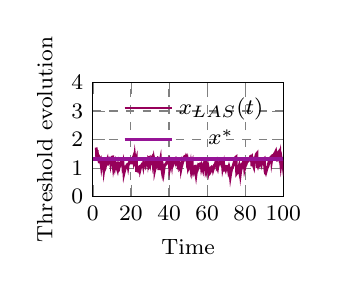
\begin{tikzpicture}
\begin{axis}[
    %title=Least-Attained-Service,
    width=0.33\textwidth,
    height=0.25\textwidth,
    xlabel={Time},
    ylabel={Threshold evolution},
    ymin=0,ymax=4,
    xmin=0,xmax=100,
    grid,
    legend pos=north east
    ]

    \addplot[color=rojito, solid, line width=1pt]
        table[row sep={\\}]        {
            \\
            1.8333333333333333  1.7219833109628464  \\
            2.0  1.3992820470981957  \\
            2.1666666666666665  1.5389630009502437  \\
            2.3333333333333335  1.6271825627457828  \\
            2.5  1.375371469366389  \\
            2.6666666666666665  1.3825373945293222  \\
            2.8333333333333335  1.38397574133321  \\
            3.0  1.3930412988082592  \\
            3.1666666666666665  1.2693225526014165  \\
            3.3333333333333335  1.215814355077569  \\
            3.5  1.213554486722253  \\
            3.6666666666666665  1.266636586738977  \\
            3.8333333333333335  1.3224145916515555  \\
            4.0  1.334557944675785  \\
            4.166666666666667  1.2181932529105333  \\
            4.333333333333333  1.154632279009304  \\
            4.5  1.0633643104716717  \\
            4.666666666666667  1.1396527252782507  \\
            4.833333333333333  1.1828379400302866  \\
            5.0  1.2024588535687717  \\
            5.166666666666667  1.2056490108300912  \\
            5.333333333333333  1.1580887924067746  \\
            5.5  1.0997537564715796  \\
            5.666666666666667  1.1196685295402076  \\
            5.833333333333333  0.9528772527230642  \\
            6.0  1.0294112711707069  \\
            6.166666666666667  1.0272537235663375  \\
            6.333333333333333  0.9709115263200836  \\
            6.5  0.996291632551206  \\
            6.666666666666667  1.0872289128633792  \\
            6.833333333333333  1.1704296901099012  \\
            7.0  1.2078801767928002  \\
            7.166666666666667  1.2369566548967077  \\
            7.333333333333333  1.2578358829155603  \\
            7.5  1.2862460880952764  \\
            7.666666666666667  1.0935951267471857  \\
            7.833333333333333  1.1802221541501394  \\
            8.0  1.2987979732031745  \\
            8.166666666666666  1.321675335907118  \\
            8.333333333333334  1.3388920816604886  \\
            8.5  1.3426059280663707  \\
            8.666666666666666  1.2846650099857906  \\
            8.833333333333334  1.252301791560041  \\
            9.0  1.2895729714348598  \\
            9.166666666666666  1.2984765781306757  \\
            9.333333333333334  1.202099525623919  \\
            9.5  1.2803615821749552  \\
            9.666666666666666  1.3233895310267183  \\
            9.833333333333334  1.3561987785114291  \\
            10.0  1.3687065801124163  \\
            10.166666666666666  1.3814037731341244  \\
            10.333333333333334  1.3927603931363812  \\
            10.5  1.393475445946855  \\
            10.666666666666666  1.1064199580697522  \\
            10.833333333333334  0.9974519614447477  \\
            11.0  1.0542245312946807  \\
            11.166666666666666  1.0713342205631622  \\
            11.333333333333334  1.1133358751767581  \\
            11.5  1.1552218610456628  \\
            11.666666666666666  1.0711356126479636  \\
            11.833333333333334  1.1312780711395694  \\
            12.0  1.06071588241202  \\
            12.166666666666666  1.071538228377314  \\
            12.333333333333334  1.102874308671752  \\
            12.5  1.1549605940216288  \\
            12.666666666666666  1.1468095654662598  \\
            12.833333333333334  0.9836090603989418  \\
            13.0  0.9452729908636006  \\
            13.166666666666666  1.0216519989797235  \\
            13.333333333333334  0.9109521408361028  \\
            13.5  0.9207063937608719  \\
            13.666666666666666  0.9867905415217184  \\
            13.833333333333334  1.0366403648346258  \\
            14.0  1.0499704667834933  \\
            14.166666666666666  1.0867607376426687  \\
            14.333333333333334  1.142914058336144  \\
            14.5  1.180854846587919  \\
            14.666666666666666  1.1965830042304404  \\
            14.833333333333334  1.2155294345873395  \\
            15.0  1.2323135704905042  \\
            15.166666666666666  1.2558787040414163  \\
            15.333333333333334  1.2716916483122471  \\
            15.5  1.2842375892165703  \\
            15.666666666666666  1.1278448423483773  \\
            15.833333333333334  1.1755683621405364  \\
            16.0  1.0212388685819227  \\
            16.166666666666668  1.0150112120504589  \\
            16.333333333333332  0.813518538760952  \\
            16.5  0.8621434768825763  \\
            16.666666666666668  0.9054656255815421  \\
            16.833333333333332  0.9362257698524084  \\
            17.0  0.9871464054827488  \\
            17.166666666666668  1.0187921923345042  \\
            17.333333333333332  1.0394164787145277  \\
            17.5  1.0379608747845053  \\
            17.666666666666668  1.0600644771201244  \\
            17.833333333333332  1.0874075711278484  \\
            18.0  1.114495602556837  \\
            18.166666666666668  1.1260315904787728  \\
            18.333333333333332  1.1310222529969178  \\
            18.5  1.0635901182201013  \\
            18.666666666666668  1.1418731528846262  \\
            18.833333333333332  1.1493436002489759  \\
            19.0  1.1780537703939542  \\
            19.166666666666668  1.206821564950463  \\
            19.333333333333332  1.2297256626203594  \\
            19.5  1.2321588828482677  \\
            19.666666666666668  1.2406116417698385  \\
            19.833333333333332  1.254787927099386  \\
            20.0  1.2605067210834  \\
            20.166666666666668  1.1337247471208993  \\
            20.333333333333332  1.2576251287336002  \\
            20.5  1.2750625731984497  \\
            20.666666666666668  1.2909706747692935  \\
            20.833333333333332  1.3102695194518077  \\
            21.0  1.3332784619735545  \\
            21.166666666666668  1.3611105686584697  \\
            21.333333333333332  1.3918301331584937  \\
            21.5  1.288257231815809  \\
            21.666666666666668  1.3469284945400322  \\
            21.833333333333332  1.302600867066205  \\
            22.0  1.4061124016151583  \\
            22.166666666666668  1.3094359315831243  \\
            22.333333333333332  1.2150962907555645  \\
            22.5  1.2359609913582972  \\
            22.666666666666668  1.2807072778665012  \\
            22.833333333333332  1.3182338022267364  \\
            23.0  0.8665958441303807  \\
            23.166666666666668  0.9299503439443111  \\
            23.333333333333332  0.9474609268418777  \\
            23.5  0.931498656949941  \\
            23.666666666666668  0.9140126378633373  \\
            23.833333333333332  0.9485641122972206  \\
            24.0  0.9788852621049149  \\
            24.166666666666668  1.0184065510157474  \\
            24.333333333333332  1.035758597927801  \\
            24.5  1.0501763825131527  \\
            24.666666666666668  1.057264894511857  \\
            24.833333333333332  0.9501091969674547  \\
            25.0  0.9949106523922611  \\
            25.166666666666668  1.0202120692354764  \\
            25.333333333333332  1.050983799150817  \\
            25.5  1.0724832541433278  \\
            25.666666666666668  1.0908277616315156  \\
            25.833333333333332  1.1224215503561004  \\
            26.0  1.1500694231619957  \\
            26.166666666666668  1.1572084072394373  \\
            26.333333333333332  1.1635338137708295  \\
            26.5  1.0923131659550438  \\
            26.666666666666668  1.1728437751358807  \\
            26.833333333333332  1.1528784638433152  \\
            27.0  1.1511651574882764  \\
            27.166666666666668  1.181230327671925  \\
            27.333333333333332  1.1892402698602424  \\
            27.5  1.1291997337463804  \\
            27.666666666666668  1.0949587572916464  \\
            27.833333333333332  1.1410856473125426  \\
            28.0  1.1979172715445738  \\
            28.166666666666668  1.2266887514281422  \\
            28.333333333333332  1.2635896476822448  \\
            28.5  1.3059554475440014  \\
            28.666666666666668  1.3376155991678829  \\
            28.833333333333332  1.3442310524220709  \\
            29.0  1.2350134476213661  \\
            29.166666666666668  1.3178162278468935  \\
            29.333333333333332  1.300001201527417  \\
            29.5  1.3379827967373472  \\
            29.666666666666668  1.3501632557739507  \\
            29.833333333333332  1.1739116963319913  \\
            30.0  1.2046059835514094  \\
            30.166666666666668  1.1461533162919793  \\
            30.333333333333332  1.2016577781382638  \\
            30.5  1.2699105853344523  \\
            30.666666666666668  1.314749835486757  \\
            30.833333333333332  1.3527968184204182  \\
            31.0  1.363269400660906  \\
            31.166666666666668  1.3796153844135848  \\
            31.333333333333332  1.4026207727620439  \\
            31.5  1.4201653214786545  \\
            31.666666666666668  1.2336963164430186  \\
            31.833333333333332  1.2990568013673605  \\
            32.0  1.2099324774861349  \\
            32.166666666666664  1.2709015778151995  \\
            32.333333333333336  1.2139724754951615  \\
            32.5  0.9296898286475042  \\
            32.666666666666664  0.9807618630500285  \\
            32.833333333333336  0.9959954202622194  \\
            33.0  1.0140837456739717  \\
            33.166666666666664  1.0667963368284021  \\
            33.333333333333336  1.159646481022678  \\
            33.5  1.233602193391188  \\
            33.666666666666664  1.2785471528577126  \\
            33.833333333333336  1.2943182005848608  \\
            34.0  1.3266765189078855  \\
            34.166666666666664  1.3506995094434977  \\
            34.333333333333336  1.343514243855529  \\
            34.5  1.3334119584215145  \\
            34.666666666666664  0.9336214009596167  \\
            34.833333333333336  1.0298711748814253  \\
            35.0  1.1150335983600075  \\
            35.166666666666664  1.1872823443317027  \\
            35.333333333333336  1.2454545298580424  \\
            35.5  1.300846686556702  \\
            35.666666666666664  1.119733322889657  \\
            35.833333333333336  1.2092799927364757  \\
            36.0  1.0270389662364963  \\
            36.166666666666664  0.9897214675649062  \\
            36.333333333333336  0.9188545562993302  \\
            36.5  1.0232390902498518  \\
            36.666666666666664  1.0802600934655993  \\
            36.833333333333336  1.023893358144778  \\
            37.0  0.9833348964957054  \\
            37.166666666666664  0.8900594724661104  \\
            37.333333333333336  0.973915014945288  \\
            37.5  1.0541867029857839  \\
            37.666666666666664  1.0799358240684769  \\
            37.833333333333336  1.097070898804162  \\
            38.0  1.1185734586402156  \\
            38.166666666666664  1.1340662310152712  \\
            38.333333333333336  1.1352190790942203  \\
            38.5  1.1503940249800035  \\
            38.666666666666664  1.178625806949849  \\
            38.833333333333336  1.2082076879387504  \\
            39.0  1.2432374973904263  \\
            39.166666666666664  1.2722290575961042  \\
            39.333333333333336  1.2978006339750765  \\
            39.5  1.32100116232212  \\
            39.666666666666664  1.347435701833481  \\
            39.833333333333336  1.3523366664002001  \\
            40.0  1.2258537436369266  \\
            40.166666666666664  1.1318027287617038  \\
            40.333333333333336  0.9725025928375219  \\
            40.5  1.0221789378061674  \\
            40.666666666666664  1.1196847343865581  \\
            40.833333333333336  1.171532704294859  \\
            41.0  1.229356119933936  \\
            41.166666666666664  1.2635631278923953  \\
            41.333333333333336  1.2401003360497997  \\
            41.5  1.1579786289589662  \\
            41.666666666666664  1.2695140424769322  \\
            41.833333333333336  1.087444895623079  \\
            42.0  1.1201063536786  \\
            42.166666666666664  1.1581655690908497  \\
            42.333333333333336  1.2233541088376478  \\
            42.5  1.2807605623882203  \\
            42.666666666666664  1.2882112418385994  \\
            42.833333333333336  1.2991270255504146  \\
            43.0  1.307737491816369  \\
            43.166666666666664  1.3278578613709051  \\
            43.333333333333336  1.3356483446617073  \\
            43.5  1.280185359454542  \\
            43.666666666666664  1.3567187833978807  \\
            43.833333333333336  1.1315623746464072  \\
            44.0  1.1321793283313153  \\
            44.166666666666664  1.224298074084829  \\
            44.333333333333336  1.2420844897493948  \\
            44.5  1.2330431269080224  \\
            44.666666666666664  1.1513135031146509  \\
            44.833333333333336  1.1887231411911077  \\
            45.0  1.1985857522618237  \\
            45.166666666666664  1.2070022693016895  \\
            45.333333333333336  1.1389402645816271  \\
            45.5  1.0018183102729203  \\
            45.666666666666664  1.0190091220234032  \\
            45.833333333333336  1.1089079763303789  \\
            46.0  1.159467847085641  \\
            46.166666666666664  1.1537693243907792  \\
            46.333333333333336  0.9950024730594718  \\
            46.5  1.055102393902716  \\
            46.666666666666664  1.1432960750336942  \\
            46.833333333333336  1.204811990797746  \\
            47.0  1.1642440656550757  \\
            47.166666666666664  1.207616139712056  \\
            47.333333333333336  1.233217600565346  \\
            47.5  1.2698969484486842  \\
            47.666666666666664  1.3123188594774193  \\
            47.833333333333336  1.361704040264816  \\
            48.0  1.3921070238303086  \\
            48.166666666666664  1.403017772076666  \\
            48.333333333333336  1.4095773718110252  \\
            48.5  1.3561025045048791  \\
            48.666666666666664  1.2433864977936686  \\
            48.833333333333336  1.3772736087356705  \\
            49.0  1.4132687407124074  \\
            49.166666666666664  1.392680111125614  \\
            49.333333333333336  1.3815397451938056  \\
            49.5  1.243559483374924  \\
            49.666666666666664  1.2868849781945162  \\
            49.833333333333336  1.2135944629915862  \\
            50.0  1.2233489505549286  \\
            50.166666666666664  1.0087528616690666  \\
            50.333333333333336  1.0383687597295057  \\
            50.5  1.0506199516972503  \\
            50.666666666666664  1.094327608302318  \\
            50.833333333333336  1.1290006063758897  \\
            51.0  1.1570954097096458  \\
            51.166666666666664  1.0868878600393257  \\
            51.333333333333336  1.1495247117831116  \\
            51.5  1.036989656102342  \\
            51.666666666666664  1.1079123593093787  \\
            51.833333333333336  1.1676976211203596  \\
            52.0  1.204460234649623  \\
            52.166666666666664  1.2326576429430807  \\
            52.333333333333336  0.9574993789182162  \\
            52.5  1.0060217369164648  \\
            52.666666666666664  0.9847573241717736  \\
            52.833333333333336  0.9390935957725506  \\
            53.0  1.0176890164912515  \\
            53.166666666666664  1.039131347812834  \\
            53.333333333333336  1.035955857348398  \\
            53.5  1.0542496094729286  \\
            53.666666666666664  1.0659315354919072  \\
            53.833333333333336  1.067141987765799  \\
            54.0  0.8423857665493841  \\
            54.166666666666664  0.7667504685116597  \\
            54.333333333333336  0.8524699603338562  \\
            54.5  0.877274633982293  \\
            54.666666666666664  0.8914716055503203  \\
            54.833333333333336  0.9357304893146601  \\
            55.0  0.9847046757624587  \\
            55.166666666666664  1.0336856272704436  \\
            55.333333333333336  1.0741956072255885  \\
            55.5  1.0548971486565777  \\
            55.666666666666664  1.092097873366149  \\
            55.833333333333336  1.1022780197834798  \\
            56.0  1.1231415175635773  \\
            56.166666666666664  1.1443952421684358  \\
            56.333333333333336  1.1490561881658614  \\
            56.5  1.1499169073811313  \\
            56.666666666666664  1.1422434479103507  \\
            56.833333333333336  1.131252095328258  \\
            57.0  1.0265691970170185  \\
            57.166666666666664  1.0752481751491811  \\
            57.333333333333336  1.033653560941483  \\
            57.5  0.9910709450942714  \\
            57.666666666666664  0.9869270655386233  \\
            57.833333333333336  0.9445412597638343  \\
            58.0  1.021789092086109  \\
            58.166666666666664  1.0872104229420279  \\
            58.333333333333336  1.1301006404123326  \\
            58.5  1.1756211266430894  \\
            58.666666666666664  1.2131091922580275  \\
            58.833333333333336  1.2432275845128682  \\
            59.0  1.2668178939301602  \\
            59.166666666666664  1.2738795291758533  \\
            59.333333333333336  0.9876976192565579  \\
            59.5  1.029944908010158  \\
            59.666666666666664  0.9362161322533289  \\
            59.833333333333336  0.9879602274877686  \\
            60.0  1.0571878880148438  \\
            60.166666666666664  1.0758603486979292  \\
            60.333333333333336  1.101555708241209  \\
            60.5  1.045222219029917  \\
            60.666666666666664  0.9897092160252687  \\
            60.833333333333336  0.8858561452481366  \\
            61.0  0.9348372625258863  \\
            61.166666666666664  0.915745278112631  \\
            61.333333333333336  0.9014370666929781  \\
            61.5  0.9621619155525567  \\
            61.666666666666664  0.9767523416496784  \\
            61.833333333333336  0.885301556339684  \\
            62.0  0.9057410036652769  \\
            62.166666666666664  0.9440242407438125  \\
            62.333333333333336  0.9814403759287744  \\
            62.5  1.002536397450263  \\
            62.666666666666664  0.9870428084342464  \\
            62.833333333333336  1.010661363144731  \\
            63.0  1.0257560973701612  \\
            63.166666666666664  0.9525876810637346  \\
            63.333333333333336  0.9892177384484298  \\
            63.5  1.0311683594243197  \\
            63.666666666666664  1.055590132007016  \\
            63.833333333333336  1.078153461607837  \\
            64.0  1.103264040443386  \\
            64.16666666666667  1.1363336257614516  \\
            64.33333333333333  1.160920674476127  \\
            64.5  1.1957488021252562  \\
            64.66666666666667  1.2331525117780355  \\
            64.83333333333333  1.2526956417920148  \\
            65.0  1.1546579766907756  \\
            65.16666666666667  1.0259300631431536  \\
            65.33333333333333  1.0436479493549056  \\
            65.5  1.007751016827783  \\
            65.66666666666667  1.0889471267784996  \\
            65.83333333333333  1.0903055588419917  \\
            66.0  1.1246950833994525  \\
            66.16666666666667  1.154011280628087  \\
            66.33333333333333  1.1830212169730885  \\
            66.5  1.2141116394017684  \\
            66.66666666666667  1.2343604879765837  \\
            66.83333333333333  1.247385752874258  \\
            67.0  1.2684400695590947  \\
            67.16666666666667  1.2934701463564418  \\
            67.33333333333333  1.2999887180803995  \\
            67.5  1.1433788309568909  \\
            67.66666666666667  1.1117403435398296  \\
            67.83333333333333  1.1225274503909306  \\
            68.0  1.1239779328155062  \\
            68.16666666666667  0.9910717946838843  \\
            68.33333333333333  1.0390728390994033  \\
            68.5  1.105869030068336  \\
            68.66666666666667  1.151480092905627  \\
            68.83333333333333  1.0318065633777729  \\
            69.0  0.9297884944397479  \\
            69.16666666666667  0.9325213589124619  \\
            69.33333333333333  0.9752197841729211  \\
            69.5  0.9959347544600079  \\
            69.66666666666667  0.9632594509835994  \\
            69.83333333333333  1.0243948979516921  \\
            70.0  1.0578301477308276  \\
            70.16666666666667  1.0589783172170826  \\
            70.33333333333333  1.0039650469701948  \\
            70.5  0.9758399375876521  \\
            70.66666666666667  0.9884339623829015  \\
            70.83333333333333  1.0230893766464981  \\
            71.0  1.027997233332183  \\
            71.16666666666667  0.9463857057527463  \\
            71.33333333333333  1.0019983249453508  \\
            71.5  1.0467137885344746  \\
            71.66666666666667  1.0059895909531065  \\
            71.83333333333333  0.9455595069646847  \\
            72.0  0.8270347672130225  \\
            72.16666666666667  0.7166290644278068  \\
            72.33333333333333  0.7912961138249566  \\
            72.5  0.8423375619468776  \\
            72.66666666666667  0.8946701060317779  \\
            72.83333333333333  0.9540038704467363  \\
            73.0  0.9795434925743005  \\
            73.16666666666667  1.0118762977104359  \\
            73.33333333333333  1.0303086844596825  \\
            73.5  1.052716569963811  \\
            73.66666666666667  1.084270137472469  \\
            73.83333333333333  1.1253841375952358  \\
            74.0  1.1564136950384722  \\
            74.16666666666667  1.20282160974101  \\
            74.33333333333333  1.2452431137410405  \\
            74.5  1.2899063734555953  \\
            74.66666666666667  1.333898389471842  \\
            74.83333333333333  1.3651085750423135  \\
            75.0  1.3807733465810885  \\
            75.16666666666667  1.3896967853072466  \\
            75.33333333333333  1.1080829595761659  \\
            75.5  0.8148035173245345  \\
            75.66666666666667  0.8312861214463025  \\
            75.83333333333333  0.8777992084909705  \\
            76.0  0.9268322726583051  \\
            76.16666666666667  0.9476516609343975  \\
            76.33333333333333  0.9808091742612168  \\
            76.5  1.0121891266867622  \\
            76.66666666666667  1.0502197051846915  \\
            76.83333333333333  0.9164988834160543  \\
            77.0  0.8610388212457911  \\
            77.16666666666667  0.9253716642613027  \\
            77.33333333333333  0.959584436557774  \\
            77.5  0.8288693856436584  \\
            77.66666666666667  0.9166202621387378  \\
            77.83333333333333  0.945384099464891  \\
            78.0  0.992850367299047  \\
            78.16666666666667  1.04150658787897  \\
            78.33333333333333  1.0738716630706246  \\
            78.5  1.1158811595597067  \\
            78.66666666666667  1.1596065501624029  \\
            78.83333333333333  1.189218651609738  \\
            79.0  1.2109038935051273  \\
            79.16666666666667  1.222790929730186  \\
            79.33333333333333  1.2351015238831389  \\
            79.5  1.1277795200992529  \\
            79.66666666666667  0.9809178532736353  \\
            79.83333333333333  1.0272490120775455  \\
            80.0  1.0799678755536166  \\
            80.16666666666667  1.0869151592823383  \\
            80.33333333333333  1.1132265290775072  \\
            80.5  1.1397860737169427  \\
            80.66666666666667  1.1854130090804098  \\
            80.83333333333333  1.2154269839531557  \\
            81.0  1.2324799935645991  \\
            81.16666666666667  1.2398098655205332  \\
            81.33333333333333  1.238816880480475  \\
            81.5  1.2502992002314928  \\
            81.66666666666667  1.2613543714837177  \\
            81.83333333333333  1.2767870463067466  \\
            82.0  1.2916177143093703  \\
            82.16666666666667  1.3039208862518088  \\
            82.33333333333333  1.3279561402012519  \\
            82.5  1.3606915173760523  \\
            82.66666666666667  1.389822039350767  \\
            82.83333333333333  1.415164618993309  \\
            83.0  1.4192091803376594  \\
            83.16666666666667  1.3212989716362318  \\
            83.33333333333333  1.3425276446467478  \\
            83.5  1.061195392905986  \\
            83.66666666666667  1.1408928340713629  \\
            83.83333333333333  1.1796041189131958  \\
            84.0  1.168110879579709  \\
            84.16666666666667  1.200823243586327  \\
            84.33333333333333  1.0873501186066508  \\
            84.5  1.0531517958278283  \\
            84.66666666666667  1.1668676443704054  \\
            84.83333333333333  1.2223168665230704  \\
            85.0  1.2770568849035144  \\
            85.16666666666667  1.3201925450181644  \\
            85.33333333333333  1.3589722798956867  \\
            85.5  1.407642931824574  \\
            85.66666666666667  1.455209256604208  \\
            85.83333333333333  1.4857775436111922  \\
            86.0  1.5051584337962378  \\
            86.16666666666667  1.5183235478630737  \\
            86.33333333333333  1.002725645010074  \\
            86.5  1.1038028842575418  \\
            86.66666666666667  1.0709166745520666  \\
            86.83333333333333  1.109623672522913  \\
            87.0  1.1636964154563216  \\
            87.16666666666667  1.19240670218997  \\
            87.33333333333333  1.2001775324792368  \\
            87.5  1.1679768185265411  \\
            87.66666666666667  1.2221868727949277  \\
            87.83333333333333  1.2318397110963542  \\
            88.0  1.234806864790115  \\
            88.16666666666667  1.2383411810901448  \\
            88.33333333333333  1.2065328026749569  \\
            88.5  1.163354866435281  \\
            88.66666666666667  1.2358024989395016  \\
            88.83333333333333  1.244504994475987  \\
            89.0  1.2573041052633034  \\
            89.16666666666667  1.269576290199776  \\
            89.33333333333333  1.2844097866031612  \\
            89.5  1.243491116389638  \\
            89.66666666666667  1.2971205955832454  \\
            89.83333333333333  1.3093556372350186  \\
            90.0  1.3212067531384268  \\
            90.16666666666667  1.178336228007978  \\
            90.33333333333333  0.9213295187209951  \\
            90.5  0.8647836447764243  \\
            90.66666666666667  0.8744654702559459  \\
            90.83333333333333  0.842517310812994  \\
            91.0  0.8814043880775717  \\
            91.16666666666667  0.9300544155080637  \\
            91.33333333333333  0.9673348634143384  \\
            91.5  1.002524939917409  \\
            91.66666666666667  1.034146803032957  \\
            91.83333333333333  1.046770879018281  \\
            92.0  1.0682119322636923  \\
            92.16666666666667  1.1234509712650613  \\
            92.33333333333333  1.1894800378857247  \\
            92.5  1.2480590502985436  \\
            92.66666666666667  1.2973481781077072  \\
            92.83333333333333  1.3190311966044779  \\
            93.0  1.3360028419321184  \\
            93.16666666666667  1.3545328197620172  \\
            93.33333333333333  1.3724170541584169  \\
            93.5  1.3866143370565498  \\
            93.66666666666667  1.3971865148988267  \\
            93.83333333333333  1.2580912241305808  \\
            94.0  1.3318881147981898  \\
            94.16666666666667  1.4015924433791709  \\
            94.33333333333333  1.4135582295876472  \\
            94.5  1.3633641484621162  \\
            94.66666666666667  1.379151638235427  \\
            94.83333333333333  1.4307713675425813  \\
            95.0  1.438367756320639  \\
            95.16666666666667  1.4636816777759218  \\
            95.33333333333333  1.4990060908741487  \\
            95.5  1.5221787943022878  \\
            95.66666666666667  1.5358269281649353  \\
            95.83333333333333  1.5540810183637663  \\
            96.0  1.5775376397359615  \\
            96.16666666666667  1.4908217625082325  \\
            96.33333333333333  1.3260591876300787  \\
            96.5  1.2971200364203805  \\
            96.66666666666667  1.2847001712432298  \\
            96.83333333333333  1.2942130310295563  \\
            97.0  1.3663621369498435  \\
            97.16666666666667  1.4569179827374192  \\
            97.33333333333333  1.5197271718445426  \\
            97.5  1.5574919501103492  \\
            97.66666666666667  1.5727153837353853  \\
            97.83333333333333  1.3489589719137172  \\
            98.0  1.4576995846107805  \\
            98.16666666666667  1.5021004035307985  \\
            98.33333333333333  1.173222908729187  \\
            98.5  1.2444646182193075  \\
            98.66666666666667  1.1298945551558202  \\
            98.83333333333333  1.2263307593203159  \\
            99.0  1.2897519319671489  \\
            99.16666666666667  1.2167877354087882  \\
            99.33333333333333  1.2269018326293377  \\
            99.5  1.1558600208598628  \\
            99.66666666666667  1.0962914466527343  \\
            99.83333333333333  1.0163282111997063  \\
            100.0  1.0043857807125054  \\
            100.16666666666667  0.9138693885802245  \\
            100.33333333333333  0.9440133481243955  \\
            100.5  1.0200775851007866  \\
            100.66666666666667  1.0592289212902708  \\
            100.83333333333333  1.109988200616713  \\
            101.0  1.1609304421481674  \\
            101.16666666666667  1.2238268544523514  \\
            101.33333333333333  1.2839045338122856  \\
            101.5  1.3300291227235663  \\
            101.66666666666667  1.3760919865921069  \\
            101.83333333333333  1.409522085455965  \\
            102.0  1.4361874785053999  \\
            102.16666666666667  1.455608404200782  \\
            102.33333333333333  1.4539668249574884  \\
            102.5  1.2636827519941214  \\
            102.66666666666667  1.0886039834990129  \\
            102.83333333333333  1.180650349857871  \\
            103.0  1.2165802715641265  \\
            103.16666666666667  1.22242181857691  \\
            103.33333333333333  1.2493592973354748  \\
            103.5  1.2290838734295877  \\
            103.66666666666667  1.1648272614247897  \\
            103.83333333333333  1.1753509342748716  \\
            104.0  1.2329822492753626  \\
            104.16666666666667  1.2514279099408245  \\
            104.33333333333333  1.1763019589589727  \\
            104.5  1.283263920224539  \\
            104.66666666666667  1.3005197445046903  \\
            104.83333333333333  1.2640431772751692  \\
            105.0  0.9678054039249985  \\
            105.16666666666667  1.1317586933457218  \\
            105.33333333333333  1.242355865350948  \\
            105.5  1.2458633984578  \\
            105.66666666666667  1.2929471915159585  \\
            105.83333333333333  1.3145577524147036  \\
            106.0  1.3349313362353463  \\
            106.16666666666667  1.3515127646366505  \\
            106.33333333333333  1.3640353599598696  \\
            106.5  1.377648874040732  \\
            106.66666666666667  1.3156324460189097  \\
            106.83333333333333  1.230418826406952  \\
            107.0  1.1894084584524764  \\
            107.16666666666667  1.2585666423485407  \\
            107.33333333333333  1.364749265359377  \\
            107.5  1.398590188862217  \\
            107.66666666666667  1.4171087040710129  \\
            107.83333333333333  1.4347562162095744  \\
            108.0  1.238733043724793  \\
            108.16666666666667  1.049979821247974  \\
            108.33333333333333  1.1068247878704005  \\
            108.5  1.1825469924044683  \\
            108.66666666666667  1.220935418137743  \\
            108.83333333333333  1.127369855037003  \\
            109.0  1.2041727998880005  \\
            109.16666666666667  1.260607555528775  \\
            109.33333333333333  1.2812345062302262  \\
            109.5  1.2977634063597647  \\
            109.66666666666667  1.138391829938524  \\
            109.83333333333333  1.110296924000468  \\
            110.0  1.1014126325743243  \\
            110.16666666666667  1.1745437550280489  \\
            110.33333333333333  1.0764329572724165  \\
            110.5  1.1383194066406748  \\
            110.66666666666667  1.1956179290613562  \\
            110.83333333333333  1.2331006778352105  \\
            111.0  1.2584552345003366  \\
            111.16666666666667  1.29055026164064  \\
            111.33333333333333  1.3092065473041812  \\
            111.5  1.3013589129916259  \\
            111.66666666666667  1.281481311118314  \\
            111.83333333333333  1.3241225875119427  \\
            112.0  1.3378395722556515  \\
            112.16666666666667  1.1554454978853677  \\
            112.33333333333333  1.1872877580702954  \\
            112.5  1.2467511621764222  \\
            112.66666666666667  1.307071001326717  \\
            112.83333333333333  1.35031639951203  \\
            113.0  1.3745442052749022  \\
            113.16666666666667  1.4010490780153892  \\
            113.33333333333333  1.4399951448828725  \\
            113.5  1.4662595784894283  \\
            113.66666666666667  1.4809048944400627  \\
            113.83333333333333  1.501667642958302  \\
            114.0  1.516058319184135  \\
            114.16666666666667  1.5215306734011833  \\
            114.33333333333333  1.0781249778763569  \\
            114.5  1.1571746304746013  \\
            114.66666666666667  1.1162580925468508  \\
            114.83333333333333  1.1470190154260607  \\
            115.0  1.1868816433501035  \\
            115.16666666666667  1.218752168393002  \\
            115.33333333333333  1.2718470590030246  \\
            115.5  1.1835120788457276  \\
            115.66666666666667  1.2184210873953565  \\
            115.83333333333333  1.2532585881864335  \\
            116.0  1.1600548616123731  \\
            116.16666666666667  1.1726415611147747  \\
            116.33333333333333  1.2240506097398764  \\
            116.5  1.100338799157583  \\
            116.66666666666667  1.185836207874406  \\
            116.83333333333333  1.1657762650300887  \\
            117.0  1.197221997955369  \\
            117.16666666666667  1.2036774839700561  \\
            117.33333333333333  1.0036044549132317  \\
            117.5  1.1092810390148211  \\
            117.66666666666667  1.1992741622378609  \\
            117.83333333333333  1.2350624503239787  \\
            118.0  1.2572912123881481  \\
            118.16666666666667  1.2898433145643082  \\
            118.33333333333333  1.31861072502711  \\
            118.5  1.3492263618945346  \\
            118.66666666666667  1.3700115531587915  \\
            118.83333333333333  1.3838530552556239  \\
            119.0  1.4007109033652183  \\
            119.16666666666667  1.4250778920562546  \\
            119.33333333333333  1.4517606302193613  \\
            119.5  1.4785675070648736  \\
            119.66666666666667  1.5162322331867992  \\
            119.83333333333333  1.5450686473353743  \\
            120.0  1.587776762411982  \\
            120.16666666666667  1.613791923426401  \\
            120.33333333333333  1.6304300140402128  \\
            120.5  1.3812390898078348  \\
            120.66666666666667  1.3507177881964072  \\
            120.83333333333333  1.2053738589958676  \\
            121.0  0.9597206866750825  \\
            121.16666666666667  0.9676432244027797  \\
            121.33333333333333  0.8996959581233308  \\
            121.5  0.9697226587597534  \\
            121.66666666666667  0.9622823084225023  \\
            121.83333333333333  0.9912700577569894  \\
            122.0  0.9975085598827054  \\
            122.16666666666667  0.9450360467510496  \\
            122.33333333333333  0.9728012642905975  \\
            122.5  0.9995062606617449  \\
            122.66666666666667  1.030882288565165  \\
            122.83333333333333  1.0876641202363817  \\
            123.0  1.1544868290997683  \\
            123.16666666666667  1.2193841143061253  \\
            123.33333333333333  1.268820859499538  \\
            123.5  1.296198954244601  \\
            123.66666666666667  1.3272945577609017  \\
            123.83333333333333  1.3200046519707  \\
            124.0  1.351583481811827  \\
            124.16666666666667  1.3623227267043294  \\
            124.33333333333333  1.1255292735030769  \\
            124.5  1.088591172459214  \\
            124.66666666666667  1.1259216151267695  \\
            124.83333333333333  1.1628118125895521  \\
            125.0  1.1874198091554713  \\
            125.16666666666667  1.2406807579592884  \\
            125.33333333333333  1.3057634824422042  \\
            125.5  1.331905798010513  \\
            125.66666666666667  1.2138745347828912  \\
            125.83333333333333  1.0447923292845331  \\
            126.0  0.9347087372523539  \\
            126.16666666666667  0.8101298446067315  \\
            126.33333333333333  0.833664545286311  \\
            126.5  0.8728502600766554  \\
            126.66666666666667  0.9213775953518784  \\
            126.83333333333333  0.9606418287010772  \\
            127.0  1.0082184900392155  \\
            127.16666666666667  1.0765510480299918  \\
            127.33333333333333  1.1314914868106096  \\
            127.5  1.1819204193898978  \\
            127.66666666666667  1.2175671967071557  \\
            127.83333333333333  1.1595392884047295  \\
            128.0  1.2252971718011314  \\
            128.16666666666666  1.2444176579467081  \\
            128.33333333333334  1.253569391912721  \\
            128.5  1.2288426535701993  \\
            128.66666666666666  1.0200543710075016  \\
            128.83333333333334  0.9752415104657772  \\
            129.0  1.0199742193538412  \\
            129.16666666666666  1.0403927840873073  \\
            129.33333333333334  1.118878556618779  \\
            129.5  1.1629962458397998  \\
            129.66666666666666  1.2304812115551211  \\
            129.83333333333334  1.227113491978884  \\
            130.0  1.1793886530405184  \\
            130.16666666666666  1.1844930311967206  \\
            130.33333333333334  1.2637720021811125  \\
            130.5  1.2883055560006313  \\
            130.66666666666666  1.3034430055122936  \\
            130.83333333333334  1.2877943730302515  \\
            131.0  1.1695941257294178  \\
            131.16666666666666  1.1583971938856914  \\
            131.33333333333334  1.0846935708412386  \\
            131.5  0.9626796746201762  \\
            131.66666666666666  0.9356569099357661  \\
            131.83333333333334  0.9712733142009397  \\
            132.0  0.960147559509295  \\
            132.16666666666666  0.9440940693164004  \\
            132.33333333333334  1.0080584154368077  \\
            132.5  1.0525111767202733  \\
            132.66666666666666  1.1115887078017526  \\
            132.83333333333334  1.15392031995942  \\
            133.0  1.1697200837450064  \\
            133.16666666666666  1.073973072721259  \\
            133.33333333333334  0.8498792209963426  \\
            133.5  1.0298315809638199  \\
            133.66666666666666  1.0395254728106802  \\
            133.83333333333334  1.1008887151088231  \\
            134.0  1.1339151145450572  \\
            134.16666666666666  1.1657786628653382  \\
            134.33333333333334  1.1863884923435548  \\
            134.5  1.1940329615606675  \\
            134.66666666666666  1.15716865548282  \\
            134.83333333333334  1.2082215270571846  \\
            135.0  1.142241377521515  \\
            135.16666666666666  1.0010200471480184  \\
            135.33333333333334  1.0719155169039705  \\
            135.5  0.9498159021877373  \\
            135.66666666666666  0.9967953106339293  \\
            135.83333333333334  1.021929551417741  \\
            136.0  1.0366059541058137  \\
            136.16666666666666  1.0841263391082196  \\
            136.33333333333334  1.1275899105743763  \\
            136.5  1.1451833399767675  \\
            136.66666666666666  1.1722109693420526  \\
            136.83333333333334  1.2045915729280807  \\
            137.0  1.2243095783147826  \\
            137.16666666666666  1.2361182250352765  \\
            137.33333333333334  1.2471490382639363  \\
            137.5  1.2496961045569304  \\
            137.66666666666666  1.2640077613453555  \\
            137.83333333333334  1.2978989010103712  \\
            138.0  1.322099380703568  \\
            138.16666666666666  1.3387593090003111  \\
            138.33333333333334  1.3445711691172266  \\
            138.5  1.3111402346423224  \\
            138.66666666666666  1.2990274832094992  \\
            138.83333333333334  1.0747441133665845  \\
            139.0  1.0469505190421788  \\
            139.16666666666666  1.017256709377506  \\
            139.33333333333334  1.0745651950311004  \\
            139.5  1.0710357709422882  \\
            139.66666666666666  1.0726092055459118  \\
            139.83333333333334  0.951687157264534  \\
            140.0  0.9288838511296542  \\
            140.16666666666666  0.7964307522111568  \\
            140.33333333333334  0.8320079911381693  \\
            140.5  0.8507506136810721  \\
            140.66666666666666  0.8715893624594373  \\
            140.83333333333334  0.8997372873577125  \\
            141.0  0.9095969922164784  \\
            141.16666666666666  0.9282435126969324  \\
            141.33333333333334  0.9469880912236355  \\
            141.5  0.9904244666138382  \\
            141.66666666666666  1.033868041634923  \\
            141.83333333333334  1.0704434064310369  \\
            142.0  1.1033932655387808  \\
            142.16666666666666  1.1375935875742167  \\
            142.33333333333334  1.1718696961933843  \\
            142.5  1.206842594985611  \\
            142.66666666666666  1.2300292847063965  \\
            142.83333333333334  1.2607180707661252  \\
            143.0  1.280396493287172  \\
            143.16666666666666  1.299704874402246  \\
            143.33333333333334  1.3062706309367316  \\
            143.5  1.3296102628495934  \\
            143.66666666666666  1.35487060359233  \\
            143.83333333333334  1.377254036433683  \\
            144.0  1.2084343614232012  \\
            144.16666666666666  1.1869975012044387  \\
            144.33333333333334  1.1270169453736685  \\
            144.5  0.9310902722420735  \\
            144.66666666666666  0.9300982593012908  \\
            144.83333333333334  0.9834893507144449  \\
            145.0  1.0422730504805866  \\
            145.16666666666666  1.0997490174553235  \\
            145.33333333333334  1.1401955282730045  \\
            145.5  1.1809741664125655  \\
            145.66666666666666  1.1488690831124018  \\
            145.83333333333334  1.1980216948540319  \\
            146.0  1.1727929845033318  \\
            146.16666666666666  1.2156586790407211  \\
            146.33333333333334  1.2538773192750994  \\
            146.5  1.2959523257974257  \\
            146.66666666666666  1.3399011405502632  \\
            146.83333333333334  1.355641522056498  \\
            147.0  1.268525163053354  \\
            147.16666666666666  1.167033033751181  \\
            147.33333333333334  1.241894104370977  \\
            147.5  1.0959002344629314  \\
            147.66666666666666  1.0383067633442247  \\
            147.83333333333334  1.0651101882905052  \\
            148.0  1.017697571449495  \\
            148.16666666666666  0.8576105615435239  \\
            148.33333333333334  0.9265505486903578  \\
            148.5  0.9537064441207613  \\
            148.66666666666666  0.9647657444747679  \\
            148.83333333333334  0.9915414817024655  \\
            149.0  1.0241343061997388  \\
            149.16666666666666  1.0619308105444611  \\
            149.33333333333334  1.1100179728386301  \\
            149.5  1.1630642283314845  \\
            149.66666666666666  1.2140450295356002  \\
            149.83333333333334  1.248817045865416  \\
            150.0  1.286267624348408  \\
            150.16666666666666  1.1683401579853983  \\
            150.33333333333334  1.154886987311268  \\
            150.5  1.204126357934068  \\
            150.66666666666666  1.233587557248256  \\
            150.83333333333334  1.2428883139288516  \\
            151.0  1.299904744182811  \\
            151.16666666666666  1.319135065259624  \\
            151.33333333333334  1.3334506107921946  \\
            151.5  1.3536958827148595  \\
            151.66666666666666  1.3040022393983008  \\
            151.83333333333334  1.0556149229176415  \\
            152.0  1.0353471749411938  \\
            152.16666666666666  1.018160328913865  \\
            152.33333333333334  1.0950939759833482  \\
            152.5  1.1707388380177342  \\
            152.66666666666666  1.0674565209422724  \\
            152.83333333333334  1.1471471424545212  \\
            153.0  1.1861633797471658  \\
            153.16666666666666  1.2121581368065182  \\
            153.33333333333334  1.250290866602576  \\
            153.5  1.2767423777259401  \\
            153.66666666666666  1.2886469273806038  \\
            153.83333333333334  1.317678383491689  \\
            154.0  1.3296183582857952  \\
            154.16666666666666  1.3349512507080181  \\
            154.33333333333334  1.3078412954795393  \\
            154.5  1.1607568982356629  \\
            154.66666666666666  1.2404765656772536  \\
            154.83333333333334  1.3400401589826823  \\
            155.0  1.3604086401265032  \\
            155.16666666666666  1.373770140371179  \\
            155.33333333333334  1.3956477893208037  \\
            155.5  1.4085052073253266  \\
            155.66666666666666  1.4273168428217886  \\
            155.83333333333334  1.447590259798527  \\
            156.0  1.4588342536371832  \\
            156.16666666666666  1.4708619480894656  \\
            156.33333333333334  1.482579798194192  \\
            156.5  1.4996982000820553  \\
            156.66666666666666  1.5169306345481797  \\
            156.83333333333334  1.5266093832848453  \\
            157.0  1.535518714741892  \\
            157.16666666666666  1.5424720096288542  \\
            157.33333333333334  1.2931574372198331  \\
            157.5  1.2739564876456217  \\
            157.66666666666666  1.381281144353989  \\
            157.83333333333334  1.4007449938582504  \\
            158.0  1.3831341543014744  \\
            158.16666666666666  1.4238654905904016  \\
            158.33333333333334  1.4489543498908901  \\
            158.5  1.4845238713174593  \\
            158.66666666666666  1.4729087295819174  \\
            158.83333333333334  1.3865394065099963  \\
            159.0  1.2696649990938624  \\
            159.16666666666666  1.256930626361253  \\
            159.33333333333334  1.1412535810552251  \\
            159.5  1.1832415028115193  \\
            159.66666666666666  0.9961618514973813  \\
            159.83333333333334  1.0649409836693136  \\
            160.0  0.9091028936601901  \\
            160.16666666666666  1.0133585822427302  \\
            160.33333333333334  1.0807467824124943  \\
            160.5  1.0681742688428528  \\
            160.66666666666666  1.1337635048941013  \\
            160.83333333333334  1.1801368813175004  \\
            161.0  1.215662632579851  \\
            161.16666666666666  1.2425315671892743  \\
            161.33333333333334  1.2684609739162185  \\
            161.5  1.2880284232251489  \\
            161.66666666666666  1.2949932932659483  \\
            161.83333333333334  1.3132927999832025  \\
            162.0  1.335461316016278  \\
            162.16666666666666  1.369391892682203  \\
            162.33333333333334  1.3973654362192596  \\
            162.5  1.1883627045332898  \\
            162.66666666666666  1.1977257161174757  \\
            162.83333333333334  1.0679251258479023  \\
            163.0  1.1591162776649702  \\
            163.16666666666666  1.233498591709818  \\
            163.33333333333334  1.265772285084993  \\
            163.5  1.2615006042366583  \\
            163.66666666666666  1.2758835420778136  \\
            163.83333333333334  1.1522140917714685  \\
            164.0  1.1378200549705773  \\
            164.16666666666666  1.3030149847750572  \\
            164.33333333333334  1.3844565807526268  \\
            164.5  1.4885904776315417  \\
            164.66666666666666  1.5754132299290209  \\
            164.83333333333334  1.7204642720912293  \\
        }
        ;
    \addlegendentry {$x_{LAS}(t)$}
        \addplot[color=violetita, solid, very thick]
        table[row sep={\\}]
        {
            \\
            0.0  1.322  \\
            100.0  1.322  \\
        }
        ;
    \addlegendentry {$x^*$}
\end{axis}
\end{tikzpicture}

%     \tikzsetnextfilename{lognormal_lcfs_threshold}
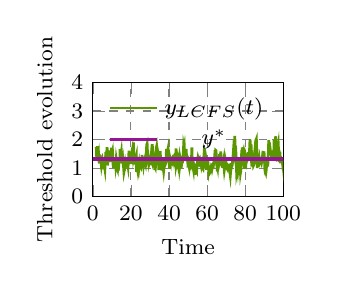
\begin{tikzpicture}
\begin{axis}[
    %title=Last-Come-First-Served,
    width=0.33\textwidth,
    height=0.25\textwidth,
    xlabel={Time},
    ylabel={Threshold evolution},
    ymin=0,ymax=4,
    xmin=0,xmax=100,
    grid,
    legend pos=north east
    ]
    \addplot[color=verdecito, solid, line width=1pt]
        table[row sep={\\}]
        {
            \\
            1.8333333333333333  1.7375836351652167  \\
            2.0  1.3992820470981964  \\
            2.1666666666666665  1.648136779008885  \\
            2.3333333333333335  1.76817082589206  \\
            2.5  1.42189631883173  \\
            2.6666666666666665  1.3942803432858542  \\
            2.8333333333333335  1.439327021821396  \\
            3.0  1.494700165874796  \\
            3.1666666666666665  1.269322552601419  \\
            3.3333333333333335  1.2158143550775766  \\
            3.5  1.2187131531157576  \\
            3.6666666666666665  1.4710887113868765  \\
            3.8333333333333335  1.399955165826836  \\
            4.0  1.3409636255976753  \\
            4.166666666666667  1.2416148404112635  \\
            4.333333333333333  1.1738502600709313  \\
            4.5  1.0837701008849892  \\
            4.666666666666667  1.1580730801540375  \\
            4.833333333333333  1.245317273545278  \\
            5.0  1.2920080782770458  \\
            5.166666666666667  1.221745320171876  \\
            5.333333333333333  1.1581778695931453  \\
            5.5  1.1405716848584246  \\
            5.666666666666667  1.1209136130880761  \\
            5.833333333333333  0.9581868084584197  \\
            6.0  1.1679467487873536  \\
            6.166666666666667  1.0418961635784267  \\
            6.333333333333333  0.97091152632008  \\
            6.5  1.1937448641143353  \\
            6.666666666666667  1.370155245742823  \\
            6.833333333333333  1.5295627370583134  \\
            7.0  1.534169399056104  \\
            7.166666666666667  1.4644628416152052  \\
            7.333333333333333  1.5659213666615228  \\
            7.5  1.7325880333281898  \\
            7.666666666666667  1.0935951267471857  \\
            7.833333333333333  1.232078195108115  \\
            8.0  1.6298039715475205  \\
            8.166666666666666  1.425591303712956  \\
            8.333333333333334  1.400465304351254  \\
            8.5  1.5671319710179201  \\
            8.666666666666666  1.2946450366280127  \\
            8.833333333333334  1.3021449090837764  \\
            9.0  1.3676687597998312  \\
            9.166666666666666  1.4660401364610056  \\
            9.333333333333334  1.2126213234463084  \\
            9.5  1.4148656585179946  \\
            9.666666666666666  1.5815323251846607  \\
            9.833333333333334  1.7131155306539174  \\
            10.0  1.4444339857668105  \\
            10.166666666666666  1.5316854226972723  \\
            10.333333333333334  1.5807558847431  \\
            10.5  1.3934754459468586  \\
            10.666666666666666  1.1125870964153233  \\
            10.833333333333334  1.0061195505301193  \\
            11.0  1.13263392412337  \\
            11.166666666666666  1.122394636422909  \\
            11.333333333333334  1.1812876154689018  \\
            11.5  1.1664411380786728  \\
            11.666666666666666  1.164442587747013  \\
            11.833333333333334  1.1846716744801018  \\
            12.0  1.0684831249378401  \\
            12.166666666666666  1.1611653279909948  \\
            12.333333333333334  1.3237737183539533  \\
            12.5  1.2580312514936942  \\
            12.666666666666666  1.1669914348508144  \\
            12.833333333333334  0.9836090603989422  \\
            13.0  0.9483941953022281  \\
            13.166666666666666  1.1087307690609922  \\
            13.333333333333334  0.9109521408361037  \\
            13.5  0.9881800738421624  \\
            13.666666666666666  1.1660463444835791  \\
            13.833333333333334  1.1720318880387754  \\
            14.0  1.2060791730071365  \\
            14.166666666666666  1.2832970288766212  \\
            14.333333333333334  1.6720318880387754  \\
            14.5  1.4133824394469467  \\
            14.666666666666666  1.495270774821984  \\
            14.833333333333334  1.4722485426275806  \\
            15.0  1.550578239192422  \\
            15.166666666666666  1.3790108331758155  \\
            15.333333333333334  1.5233373705947102  \\
            15.5  1.3997675221638985  \\
            15.666666666666666  1.1498598799767237  \\
            15.833333333333334  1.2314634857003206  \\
            16.0  1.088096876542675  \\
            16.166666666666668  1.0179636792475666  \\
            16.333333333333332  0.8640823663617709  \\
            16.5  0.9212325906783327  \\
            16.666666666666668  0.9368948722893986  \\
            16.833333333333332  1.1142891152906298  \\
            17.0  1.1910448818158805  \\
            17.166666666666668  1.1222720561897823  \\
            17.333333333333332  1.0959376225923094  \\
            17.5  1.0868513309605916  \\
            17.666666666666668  1.2194150588280301  \\
            17.833333333333332  1.2592847774212572  \\
            18.0  1.3438190880736052  \\
            18.166666666666668  1.1372767897825433  \\
            18.333333333333332  1.1368176214590981  \\
            18.5  1.063590118220091  \\
            18.666666666666668  1.230256784886759  \\
            18.833333333333332  1.3969234515534232  \\
            19.0  1.6074089555136872  \\
            19.166666666666668  1.5084670473475832  \\
            19.333333333333332  1.4135854581682814  \\
            19.5  1.234190777254696  \\
            19.666666666666668  1.3716177413934219  \\
            19.833333333333332  1.3664066835175426  \\
            20.0  1.3673207682340092  \\
            20.166666666666668  1.1419003814301973  \\
            20.333333333333332  1.3085670480968616  \\
            20.5  1.3626000895734123  \\
            20.666666666666668  1.6260990167398148  \\
            20.833333333333332  1.6793293858467386  \\
            21.0  1.5638601460987225  \\
            21.166666666666668  1.7386035926490955  \\
            21.333333333333332  1.8971934794320546  \\
            21.5  1.3100915489404805  \\
            21.666666666666668  1.3491750647319272  \\
            21.833333333333332  1.364008536195815  \\
            22.0  1.470252426188285  \\
            22.166666666666668  1.309435931583124  \\
            22.333333333333332  1.222000956888877  \\
            22.5  1.2364034293867974  \\
            22.666666666666668  1.357946074802232  \\
            22.833333333333332  1.4100414329665298  \\
            23.0  0.8665958441303871  \\
            23.166666666666668  1.0134325690747303  \\
            23.333333333333332  0.9626746832170028  \\
            23.5  1.0412662862995106  \\
            23.666666666666668  0.9481384752286068  \\
            23.833333333333332  1.0337490375392022  \\
            24.0  1.1381471667305405  \\
            24.166666666666668  1.1930954485030654  \\
            24.333333333333332  1.0651563553267316  \\
            24.5  1.1564617055627764  \\
            24.666666666666668  1.1313394943452657  \\
            24.833333333333332  0.9823124808971464  \\
            25.0  1.0855430132321402  \\
            25.166666666666668  1.0596237391164216  \\
            25.333333333333332  1.1960728779533802  \\
            25.5  1.1715899897310038  \\
            25.666666666666668  1.2973411246856088  \\
            25.833333333333332  1.464007791352273  \\
            26.0  1.2695319291306149  \\
            26.166666666666668  1.2573298001031255  \\
            26.333333333333332  1.1635338137708295  \\
            26.5  1.0923131659550407  \\
            26.666666666666668  1.1980096883334141  \\
            26.833333333333332  1.1613849390858597  \\
            27.0  1.1523361452539298  \\
            27.166666666666668  1.2704218637089753  \\
            27.333333333333332  1.31838856230803  \\
            27.5  1.1337826729018943  \\
            27.666666666666668  1.1014110736692047  \\
            27.833333333333332  1.211450074159405  \\
            28.0  1.3781167408260728  \\
            28.166666666666668  1.6622404204098373  \\
            28.333333333333332  1.8289070870765016  \\
            28.5  1.860145363019761  \\
            28.666666666666668  1.5860398238290436  \\
            28.833333333333332  1.3895028817809383  \\
            29.0  1.3061604027254  \\
            29.166666666666668  1.4545218432769644  \\
            29.333333333333332  1.332621090445258  \\
            29.5  1.3731216147543535  \\
            29.666666666666668  1.4437757252782468  \\
            29.833333333333332  1.1779689336030827  \\
            30.0  1.207322725680644  \\
            30.166666666666668  1.1969033981795079  \\
            30.333333333333332  1.40006713285889  \\
            30.5  1.45002386835451  \\
            30.666666666666668  1.560167887631529  \\
            30.833333333333332  1.560703626950236  \\
            31.0  1.7145079047159868  \\
            31.166666666666668  1.8331385011294685  \\
            31.333333333333332  1.7051625642641426  \\
            31.5  1.5355297685017142  \\
            31.666666666666668  1.2575961310117876  \\
            31.833333333333332  1.2993574299446315  \\
            32.0  1.2266586484835145  \\
            32.166666666666664  1.291904970765433  \\
            32.333333333333336  1.2139724754951793  \\
            32.5  0.929689828647529  \\
            32.666666666666664  1.0335685467829876  \\
            32.833333333333336  1.0066593827907937  \\
            33.0  1.1203630367286905  \\
            33.166666666666664  1.4342497987328677  \\
            33.333333333333336  1.7068882620891586  \\
            33.5  1.7598376171497137  \\
            33.666666666666664  1.6326634188748557  \\
            33.833333333333336  1.3773664240710204  \\
            34.0  1.5986071006510585  \\
            34.166666666666664  1.536337520203574  \\
            34.333333333333336  1.3580179781262487  \\
            34.5  1.33341195842155  \\
            34.666666666666664  0.9336214009596304  \\
            34.833333333333336  1.0797357645771726  \\
            35.0  1.3183883720464777  \\
            35.166666666666664  1.5013836300211452  \\
            35.333333333333336  1.6002880676263018  \\
            35.5  1.4115871952397256  \\
            35.666666666666664  1.1201798322431173  \\
            35.833333333333336  1.2642936498144621  \\
            36.0  1.0333367880520754  \\
            36.166666666666664  1.031230665643868  \\
            36.333333333333336  0.9188545562993227  \\
            36.5  1.1367964401922706  \\
            36.666666666666664  1.1303519569985525  \\
            36.833333333333336  1.0362848017024149  \\
            37.0  0.9858101363801097  \\
            37.166666666666664  0.9007148089034871  \\
            37.333333333333336  1.0064303105386827  \\
            37.5  1.2983088972626433  \\
            37.666666666666664  1.1320075490166062  \\
            37.833333333333336  1.281027416467147  \\
            38.0  1.1824056721392466  \\
            38.166666666666664  1.1535668749939987  \\
            38.333333333333336  1.1849879504386251  \\
            38.5  1.3665741869847423  \\
            38.666666666666664  1.6691419065510544  \\
            38.833333333333336  1.5283557881123926  \\
            39.0  1.5285323874537369  \\
            39.166666666666664  1.5108109154411835  \\
            39.333333333333336  1.6186610528514578  \\
            39.5  1.676043452975648  \\
            39.666666666666664  1.518954730259658  \\
            39.833333333333336  1.4077456017944527  \\
            40.0  1.2258537436369181  \\
            40.166666666666664  1.1318027287616914  \\
            40.333333333333336  0.9725025928375217  \\
            40.5  1.0981471192679848  \\
            40.666666666666664  1.2965710051443367  \\
            40.833333333333336  1.242509214049214  \\
            41.0  1.402503911974975  \\
            41.166666666666664  1.2894057549912006  \\
            41.333333333333336  1.2401003360498066  \\
            41.5  1.2178382716182767  \\
            41.666666666666664  1.3996080339576906  \\
            41.833333333333336  1.0884880502995102  \\
            42.0  1.204611156002784  \\
            42.166666666666664  1.2811227933344966  \\
            42.333333333333336  1.4118064085574673  \\
            42.5  1.409735777983009  \\
            42.666666666666664  1.3156530961892585  \\
            42.833333333333336  1.4044250877083613  \\
            43.0  1.4545315225091713  \\
            43.166666666666664  1.4860973643769597  \\
            43.333333333333336  1.5003568647625798  \\
            43.5  1.280185359454535  \\
            43.666666666666664  1.6925590167535773  \\
            43.833333333333336  1.1315623746463999  \\
            44.0  1.1882158144796904  \\
            44.166666666666664  1.348515205954783  \\
            44.333333333333336  1.2548489383352432  \\
            44.5  1.241051044304271  \\
            44.666666666666664  1.1696477391354136  \\
            44.833333333333336  1.2761083975602787  \\
            45.0  1.2071460834904215  \\
            45.166666666666664  1.2070022693016824  \\
            45.333333333333336  1.1389402645816205  \\
            45.5  1.0018183102729168  \\
            45.666666666666664  1.0873559911445483  \\
            45.833333333333336  1.3501030683088686  \\
            46.0  1.292354372798009  \\
            46.166666666666664  1.1537693243907654  \\
            46.333333333333336  0.9950024730594578  \\
            46.5  1.0870636792388382  \\
            46.666666666666664  1.2550419451862282  \\
            46.833333333333336  1.4217086118528997  \\
            47.0  1.167268512815241  \\
            47.166666666666664  1.3309107323217475  \\
            47.333333333333336  1.360198337624702  \\
            47.5  1.527046747310166  \\
            47.666666666666664  1.769078803043513  \\
            47.833333333333336  1.707246933566509  \\
            48.0  1.764199200282313  \\
            48.166666666666664  1.499431746772899  \\
            48.333333333333336  1.4289814397545086  \\
            48.5  1.436713342955322  \\
            48.666666666666664  1.246587141134519  \\
            48.833333333333336  1.5817374305411604  \\
            49.0  1.672710387518208  \\
            49.166666666666664  1.3956383060148099  \\
            49.333333333333336  1.381539745193784  \\
            49.5  1.2435594833749022  \\
            49.666666666666664  1.3811157798846878  \\
            49.833333333333336  1.2135944629915656  \\
            50.0  1.2430877953549029  \\
            50.166666666666664  1.0265446224407953  \\
            50.333333333333336  1.1101015057679646  \\
            50.5  1.057051652667468  \\
            50.666666666666664  1.2237183193341323  \\
            50.833333333333336  1.2288888214558682  \\
            51.0  1.1686596766923572  \\
            51.166666666666664  1.1334348573115918  \\
            51.333333333333336  1.2806507793740423  \\
            51.5  1.050417769598468  \\
            51.666666666666664  1.1885782784086203  \\
            51.833333333333336  1.3855886430058888  \\
            52.0  1.72723370965209  \\
            52.166666666666664  1.2698801306839158  \\
            52.333333333333336  0.963195116255342  \\
            52.5  1.0475050704149425  \\
            52.666666666666664  1.0170898741571293  \\
            52.833333333333336  0.9499555129128296  \\
            53.0  1.116622179579494  \\
            53.166666666666664  1.0680719562068504  \\
            53.333333333333336  1.0359558573484051  \\
            53.5  1.1152168790233006  \\
            53.666666666666664  1.1057110306923121  \\
            53.833333333333336  1.089915002830267  \\
            54.0  0.8602847966080276  \\
            54.166666666666664  0.7717069144899824  \\
            54.333333333333336  0.9227132168579146  \\
            54.5  0.8963158529549347  \\
            54.666666666666664  1.0813998006312957  \\
            54.833333333333336  1.0857546671602734  \\
            55.0  1.3123833066090995  \\
            55.166666666666664  1.3745062106951167  \\
            55.333333333333336  1.333147934035125  \\
            55.5  1.0561736404608268  \\
            55.666666666666664  1.180223530197317  \\
            55.833333333333336  1.3149333936367071  \\
            56.0  1.332789223992755  \\
            56.166666666666664  1.2523107038024506  \\
            56.333333333333336  1.161465570689991  \\
            56.5  1.1780303847593032  \\
            56.666666666666664  1.2001583364551394  \\
            56.833333333333336  1.1312520953282785  \\
            57.0  1.0665504481699841  \\
            57.166666666666664  1.1190687274084823  \\
            57.333333333333336  1.043208048400821  \\
            57.5  0.9910709450942718  \\
            57.666666666666664  0.9869270655386231  \\
            57.833333333333336  0.9700576766944522  \\
            58.0  1.1650841610525973  \\
            58.166666666666664  1.3317508277192616  \\
            58.333333333333336  1.4310354093753546  \\
            58.5  1.5977020760420189  \\
            58.666666666666664  1.5580021233409767  \\
            58.833333333333336  1.5709411591883722  \\
            59.0  1.5223822220162901  \\
            59.166666666666664  1.399318009827475  \\
            59.333333333333336  0.9876976192565508  \\
            59.5  1.0550950324135755  \\
            59.666666666666664  0.9379416420067983  \\
            59.833333333333336  1.1046083086734697  \\
            60.0  1.0906044481667792  \\
            60.166666666666664  1.147079134860725  \\
            60.333333333333336  1.3137458015273964  \\
            60.5  1.0452222190299025  \\
            60.666666666666664  1.0147800649491785  \\
            60.833333333333336  0.895524001269699  \\
            61.0  0.965577280901762  \\
            61.166666666666664  0.9157452781126452  \\
            61.333333333333336  0.901437066692985  \\
            61.5  1.0080372372339568  \\
            61.666666666666664  0.9974908971249263  \\
            61.833333333333336  0.8853015563396838  \\
            62.0  0.9057410036652769  \\
            62.166666666666664  1.0038181340604453  \\
            62.333333333333336  1.1017389919975997  \\
            62.5  1.0931756558320913  \\
            62.666666666666664  1.0106469465258314  \\
            62.833333333333336  1.070069867496727  \\
            63.0  1.1030887722274656  \\
            63.166666666666664  0.9965611936166212  \\
            63.333333333333336  1.137974744796466  \\
            63.5  1.1655849717904303  \\
            63.666666666666664  1.1889654583157991  \\
            63.833333333333336  1.3429372710700918  \\
            64.0  1.433922819303426  \\
            64.16666666666667  1.6284027242775423  \\
            64.33333333333333  1.4543258284996554  \\
            64.5  1.6209924951663268  \\
            64.66666666666667  1.6108403600052483  \\
            64.83333333333333  1.319107063089291  \\
            65.0  1.1663823190410483  \\
            65.16666666666667  1.040962580442553  \\
            65.33333333333333  1.0633513057229749  \\
            65.5  1.007751016827811  \\
            65.66666666666667  1.1683214718634503  \\
            65.83333333333333  1.156530767017884  \\
            66.0  1.3253957403159973  \\
            66.16666666666667  1.4216892888301942  \\
            66.33333333333333  1.2794178115783268  \\
            66.5  1.4882118847233698  \\
            66.66666666666667  1.29164035308888  \\
            66.83333333333333  1.3464057532481917  \\
            67.0  1.4592727777299928  \\
            67.16666666666667  1.583895552838058  \\
            67.33333333333333  1.2999887180803853  \\
            67.5  1.1527554467035515  \\
            67.66666666666667  1.1125235299347196  \\
            67.83333333333333  1.1240525393590843  \\
            68.0  1.1239779328154924  \\
            68.16666666666667  1.0088184891618113  \\
            68.33333333333333  1.1754851558284685  \\
            68.5  1.2228204370076412  \\
            68.66666666666667  1.2850969219409052  \\
            68.83333333333333  1.0439366360846378  \\
            69.0  0.9297884944397197  \\
            69.16666666666667  1.0061940305280075  \\
            69.33333333333333  1.0421049853294306  \\
            69.5  1.0917636493521883  \\
            69.66666666666667  0.992906043850823  \\
            69.83333333333333  1.226526447548025  \\
            70.0  1.1749212207513864  \\
            70.16666666666667  1.0589783172170968  \\
            70.33333333333333  1.0039650469701797  \\
            70.5  0.9830120824920385  \\
            70.66666666666667  1.0979907809357172  \\
            70.83333333333333  1.0806004534678095  \\
            71.0  1.0514426054329107  \\
            71.16666666666667  0.9539832718749466  \\
            71.33333333333333  1.1073048853965446  \\
            71.5  1.108927415837826  \\
            71.66666666666667  1.0070478424190838  \\
            71.83333333333333  0.9577551688281005  \\
            72.0  0.8363628826509597  \\
            72.16666666666667  0.749202695186554  \\
            72.33333333333333  0.8832957310944636  \\
            72.5  0.9530060888762222  \\
            72.66666666666667  1.179387962276877  \\
            72.83333333333333  1.0477722819517936  \\
            73.0  1.0726202127116267  \\
            73.16666666666667  1.096882474290723  \\
            73.33333333333333  1.23973846983219  \\
            73.5  1.2970500074308546  \\
            73.66666666666667  1.467564571521251  \\
            73.83333333333333  1.6303833407641832  \\
            74.0  1.5703281629699717  \\
            74.16666666666667  1.963716674097526  \\
            74.33333333333333  1.6657419470669907  \\
            74.5  2.129440723593177  \\
            74.66666666666667  1.7798041787628307  \\
            74.83333333333333  1.6265735014835059  \\
            75.0  1.6436010502415854  \\
            75.16666666666667  1.4771974078141596  \\
            75.33333333333333  1.1080829595761799  \\
            75.5  0.8148035173245347  \\
            75.66666666666667  0.8720757776520571  \\
            75.83333333333333  1.003688130717677  \\
            76.0  1.0641382078114816  \\
            76.16666666666667  0.9535949541224937  \\
            76.33333333333333  1.0614392311940009  \\
            76.5  1.226304969200072  \\
            76.66666666666667  1.366733703971292  \\
            76.83333333333333  0.9164988834160681  \\
            77.0  0.8981195719105983  \\
            77.16666666666667  1.012668886734474  \\
            77.33333333333333  1.0568433453124726  \\
            77.5  0.8445990701858932  \\
            77.66666666666667  0.9166202621387356  \\
            77.83333333333333  1.0545447518090612  \\
            78.0  1.3288693856436566  \\
            78.16666666666667  1.2888499768249346  \\
            78.33333333333333  1.419010123476184  \\
            78.5  1.7281882498526215  \\
            78.66666666666667  1.5433172670079927  \\
            78.83333333333333  1.4988618809715746  \\
            79.0  1.5468110695528594  \\
            79.16666666666667  1.3872251477115185  \\
            79.33333333333333  1.426603010384511  \\
            79.5  1.135155833692167  \\
            79.66666666666667  0.9809178532736382  \\
            79.83333333333333  1.088078890265038  \\
            80.0  1.0887065784382486  \\
            80.16666666666667  1.1572062308555218  \\
            80.33333333333333  1.1338679680680457  \\
            80.5  1.3423885549345158  \\
            80.66666666666667  1.2936020194811704  \\
            80.83333333333333  1.2485346187146291  \\
            81.0  1.2770901598088926  \\
            81.16666666666667  1.4374391846738064  \\
            81.33333333333333  1.2490987286879403  \\
            81.5  1.3883661084082917  \\
            81.66666666666667  1.555032775074963  \\
            81.83333333333333  1.4313088930487226  \\
            82.0  1.4165652933552195  \\
            82.16666666666667  1.4758468986709943  \\
            82.33333333333333  1.7425819922032133  \\
            82.5  1.9988584381444952  \\
            82.66666666666667  1.8756319399790584  \\
            82.83333333333333  1.611645210785511  \\
            83.0  1.4402309089234677  \\
            83.16666666666667  1.3217754450760708  \\
            83.33333333333333  1.3852336480788523  \\
            83.5  1.0611953929060007  \\
            83.66666666666667  1.1530075665999817  \\
            83.83333333333333  1.2579040698963126  \\
            84.0  1.2446537003610132  \\
            84.16666666666667  1.2164119554216342  \\
            84.33333333333333  1.087350118606679  \\
            84.5  1.1101198081683066  \\
            84.66666666666667  1.276786474834978  \\
            84.83333333333333  1.4699290190814907  \\
            85.0  1.5847835712887814  \\
            85.16666666666667  1.534019327335855  \\
            85.33333333333333  1.7925660010008642  \\
            85.5  1.9735143418034227  \\
            85.66666666666667  1.982269046697425  \\
            85.83333333333333  2.012393193809771  \\
            86.0  1.6123202862164163  \\
            86.16666666666667  1.6745767538007783  \\
            86.33333333333333  1.0043001352227776  \\
            86.5  1.2112289368534022  \\
            86.66666666666667  1.0868514984615274  \\
            86.83333333333333  1.2026368408188546  \\
            87.0  1.2919049497859731  \\
            87.16666666666667  1.248371168752712  \\
            87.33333333333333  1.312899105405208  \\
            87.5  1.1928014239720852  \\
            87.66666666666667  1.3763855653509154  \\
            87.83333333333333  1.255498707848659  \\
            88.0  1.2891435562415978  \\
            88.16666666666667  1.2925877359417086  \\
            88.33333333333333  1.2115155234896093  \\
            88.5  1.1775943986312285  \\
            88.66666666666667  1.2420614913440602  \\
            88.83333333333333  1.3512825272667328  \\
            89.0  1.396070370550973  \\
            89.16666666666667  1.4771100198520628  \\
            89.33333333333333  1.6041927572767634  \\
            89.5  1.2439641401616512  \\
            89.66666666666667  1.4145791789463118  \\
            89.83333333333333  1.581245845612969  \\
            90.0  1.4503481503575841  \\
            90.16666666666667  1.1783362280079785  \\
            90.33333333333333  0.9213295187209809  \\
            90.5  0.8660693633613477  \\
            90.66666666666667  0.883503897382198  \\
            90.83333333333333  0.8447563573157453  \\
            91.0  0.926403784395049  \\
            91.16666666666667  1.0735908292898984  \\
            91.33333333333333  1.1425240998465114  \\
            91.5  1.2067762151999943  \\
            91.66666666666667  1.3107733855004398  \\
            91.83333333333333  1.052836062847959  \\
            92.0  1.4171775294131237  \\
            92.16666666666667  1.6021504351482747  \\
            92.33333333333333  1.977440052167097  \\
            92.5  1.7869508569716146  \\
            92.66666666666667  1.6438167913967305  \\
            92.83333333333333  1.5719280422344042  \\
            93.0  1.5801384860924657  \\
            93.16666666666667  1.6268368363913908  \\
            93.33333333333333  1.5365658038312375  \\
            93.5  1.5003911246287203  \\
            93.66666666666667  1.5864998553155374  \\
            93.83333333333333  1.2580912241305953  \\
            94.0  1.3356450454139122  \\
            94.16666666666667  1.5023117120805836  \\
            94.33333333333333  1.614212432295588  \\
            94.5  1.385511533686966  \\
            94.66666666666667  1.3949099753328085  \\
            94.83333333333333  1.5362993572515649  \\
            95.0  1.5712370990858915  \\
            95.16666666666667  1.989835867163606  \\
            95.33333333333333  1.90457043241922  \\
            95.5  1.7309974876300487  \\
            95.66666666666667  1.7526936520945355  \\
            95.83333333333333  2.0093925931722367  \\
            96.0  2.11395869464711  \\
            96.16666666666667  1.4908217625082187  \\
            96.33333333333333  1.3260591876300794  \\
            96.5  1.297120036420381  \\
            96.66666666666667  1.3050693924374457  \\
            96.83333333333333  1.298248168010332  \\
            97.0  1.5624155179541361  \\
            97.16666666666667  1.749110410833154  \\
            97.33333333333333  1.818642387893732  \\
            97.5  1.5574919501103466  \\
            97.66666666666667  1.6440555634735858  \\
            97.83333333333333  1.3489589719137172  \\
            98.0  1.4630689749089498  \\
            98.16666666666667  1.5754343155775956  \\
            98.33333333333333  1.1732229087291586  \\
            98.5  1.4141013197405954  \\
            98.66666666666667  1.1702492858806437  \\
            98.83333333333333  1.3443098947337688  \\
            99.0  1.321114878997136  \\
            99.16666666666667  1.2550356531740192  \\
            99.33333333333333  1.2269018326293093  \\
            99.5  1.1633856665007016  \\
            99.66666666666667  1.111926726479311  \\
            99.83333333333333  1.0163282111997205  \\
            100.0  1.0268675072660898  \\
            100.16666666666667  0.9138693885802383  \\
            100.33333333333333  1.0049666084555753  \\
            100.5  1.063746787722323  \\
            100.66666666666667  1.2304134543889944  \\
            100.83333333333333  1.4191718224287513  \\
            101.0  1.5858384890954227  \\
            101.16666666666667  1.6910083220734577  \\
            101.33333333333333  1.9191718224287513  \\
            101.5  2.0243416554067863  \\
            101.66666666666667  1.94116913357891  \\
            101.83333333333333  1.851236505496388  \\
            102.0  1.8169966608964074  \\
            102.16666666666667  1.512245254473143  \\
            102.33333333333333  1.465296019671868  \\
            102.5  1.2636827519941392  \\
            102.66666666666667  1.0886039834990129  \\
            102.83333333333333  1.2297194182826985  \\
            103.0  1.256074561455037  \\
            103.16666666666667  1.22244545554301  \\
            103.33333333333333  1.3747459325545321  \\
            103.5  1.2290838734296017  \\
            103.66666666666667  1.1648272614248043  \\
            103.83333333333333  1.2661520236666064  \\
            104.0  1.3338576074624342  \\
            104.16666666666667  1.4161391278763347  \\
            104.33333333333333  1.1885544209225856  \\
            104.5  1.3766761856795  \\
            104.66666666666667  1.3727859723610578  \\
            104.83333333333333  1.264043177275198  \\
            105.0  0.9678054039250128  \\
            105.16666666666667  1.202312858621326  \\
            105.33333333333333  1.3010048963953267  \\
            105.5  1.261996909478185  \\
            105.66666666666667  1.4425485595035212  \\
            105.83333333333333  1.4850525124770684  \\
            106.0  1.5014143179759856  \\
            106.16666666666667  1.4567571466830458  \\
            106.33333333333333  1.391202844757231  \\
            106.5  1.5504409218085158  \\
            106.66666666666667  1.3156324460189381  \\
            106.83333333333333  1.2469586481057888  \\
            107.0  1.2247916900508926  \\
            107.16666666666667  1.3467574112544582  \\
            107.33333333333333  1.7459686500669847  \\
            107.5  1.582537442062275  \\
            107.66666666666667  1.759440011472563  \\
            107.83333333333333  1.7073766801876786  \\
            108.0  1.2387330437248494  \\
            108.16666666666667  1.0536763494620374  \\
            108.33333333333333  1.1783957533028655  \\
            108.5  1.3669446430685213  \\
            108.66666666666667  1.2375614814364582  \\
            108.83333333333333  1.1273698550370312  \\
            109.0  1.297628708237184  \\
            109.16666666666667  1.669273066740459  \\
            109.33333333333333  1.4772028055742084  \\
            109.5  1.3763149833340265  \\
            109.66666666666667  1.1386992782348813  \\
            109.83333333333333  1.1334886057694575  \\
            110.0  1.196218346051495  \\
            110.16666666666667  1.333960858713695  \\
            110.33333333333333  1.0764329572724023  \\
            110.5  1.2234179319321044  \\
            110.66666666666667  1.4897760519537684  \\
            110.83333333333333  1.3333214554102284  \\
            111.0  1.3733316367108586  \\
            111.16666666666667  1.380696015350651  \\
            111.33333333333333  1.528910151990985  \\
            111.5  1.3367974710607058  \\
            111.66666666666667  1.2814813111183412  \\
            111.83333333333333  1.5073050769490663  \\
            112.0  1.4600136293754247  \\
            112.16666666666667  1.1626480396980838  \\
            112.33333333333333  1.224696496582098  \\
            112.5  1.3003009068059868  \\
            112.66666666666667  1.4669675734726582  \\
            112.83333333333333  1.4888492213781888  \\
            113.0  1.6555158880448602  \\
            113.16666666666667  1.8157307276220251  \\
            113.33333333333333  2.0959775482625105  \\
            113.5  1.557903331227692  \\
            113.66666666666667  1.7877814227144029  \\
            113.83333333333333  1.763990484677251  \\
            114.0  1.6805892740745776  \\
            114.16666666666667  1.722634181346848  \\
            114.33333333333333  1.078124977876385  \\
            114.5  1.1699265685189175  \\
            114.66666666666667  1.1198091252749407  \\
            114.83333333333333  1.286475791941598  \\
            115.0  1.424403532352386  \\
            115.16666666666667  1.6810241813409164  \\
            115.33333333333333  1.4064321859147384  \\
            115.5  1.197247335286363  \\
            115.66666666666667  1.229041976183396  \\
            115.83333333333333  1.3322205655245654  \\
            116.0  1.1600548616123803  \\
            116.16666666666667  1.1936346829778586  \\
            116.33333333333333  1.2991304881189478  \\
            116.5  1.1087278690853282  \\
            116.66666666666667  1.2573598136181374  \\
            116.83333333333333  1.1752158017756358  \\
            117.0  1.2374657237498923  \\
            117.16666666666667  1.2411478399379376  \\
            117.33333333333333  1.012831349170284  \\
            117.5  1.1421591708581644  \\
            117.66666666666667  1.3088258375248358  \\
            117.83333333333333  1.4214950914238642  \\
            118.0  1.5368513464828908  \\
            118.16666666666667  1.6207930780420554  \\
            118.33333333333333  1.4423119249972558  \\
            118.5  1.585537185052118  \\
            118.66666666666667  1.524542340799627  \\
            118.83333333333333  1.5774954235396876  \\
            119.0  1.8952914404886627  \\
            119.16666666666667  1.9717803716194737  \\
            119.33333333333333  1.9241353071534775  \\
            119.5  2.3051137049528023  \\
            119.66666666666667  2.2574686404868203  \\
            119.83333333333333  1.869976339320914  \\
            120.0  2.0528661257444725  \\
            120.16666666666667  1.8930531387530465  \\
            120.33333333333333  1.7184000556474786  \\
            120.5  1.3815636465147918  \\
            120.66666666666667  1.3647928921938188  \\
            120.83333333333333  1.220983638358632  \\
            121.0  0.9690533509502757  \\
            121.16666666666667  0.9927632688167165  \\
            121.33333333333333  0.8996959581233313  \\
            121.5  1.0630285783360591  \\
            121.66666666666667  0.9684365982746357  \\
            121.83333333333333  1.036154084993143  \\
            122.0  1.0651655021116397  \\
            122.16666666666667  0.9879460429372671  \\
            122.33333333333333  0.9804561274739712  \\
            122.5  1.0749236451130884  \\
            122.66666666666667  1.258765873812706  \\
            122.83333333333333  1.4804561274739712  \\
            123.0  1.6689409406411357  \\
            123.16666666666667  1.665723676928124  \\
            123.33333333333333  1.6702014852889278  \\
            123.5  1.623850131901392  \\
            123.66666666666667  1.6394820880294105  \\
            123.83333333333333  1.3282039232860399  \\
            124.0  1.409986152164521  \\
            124.16666666666667  1.4386467627786317  \\
            124.33333333333333  1.1425726949702835  \\
            124.5  1.0943946794182438  \\
            124.66666666666667  1.2431591798812036  \\
            124.83333333333333  1.2297874295124984  \\
            125.0  1.4137288812514015  \\
            125.16666666666667  1.6023270615708896  \\
            125.33333333333333  1.5217514878661547  \\
            125.5  1.5836563876370349  \\
            125.66666666666667  1.2404502264848816  \\
            125.83333333333333  1.0491216288595098  \\
            126.0  0.97626493732146  \\
            126.16666666666667  0.819425835897519  \\
            126.33333333333333  0.857880866116588  \\
            126.5  0.96759444828308  \\
            126.66666666666667  1.0731641178307854  \\
            126.83333333333333  1.096993698904484  \\
            127.0  1.2636603655711554  \\
            127.16666666666667  1.4303270322378268  \\
            127.33333333333333  1.4772030703690007  \\
            127.5  1.4010190273405385  \\
            127.66666666666667  1.3911717061261584  \\
            127.83333333333333  1.1643816552524697  \\
            128.0  1.269565007067584  \\
            128.16666666666666  1.4324547692787348  \\
            128.33333333333334  1.2813934474723254  \\
            128.5  1.2552293524332612  \\
            128.66666666666666  1.0267336849619824  \\
            128.83333333333334  0.9996719338729463  \\
            129.0  1.110560477224368  \\
            129.16666666666666  1.370752558024762  \\
            129.33333333333334  1.2787565772855487  \\
            129.5  1.445423243952206  \\
            129.66666666666666  1.5457810250416912  \\
            129.83333333333334  1.2271134919787698  \\
            130.0  1.1796756972256617  \\
            130.16666666666666  1.2010450310088459  \\
            130.33333333333334  1.5540729407019853  \\
            130.5  1.5279018764637442  \\
            130.66666666666666  1.3799176775128785  \\
            130.83333333333334  1.2877943730302661  \\
            131.0  1.169594125729418  \\
            131.16666666666666  1.2323236046435966  \\
            131.33333333333334  1.0901426386263893  \\
            131.5  0.9673041091799348  \\
            131.66666666666666  0.9618271043610207  \\
            131.83333333333334  1.0215194400780376  \\
            132.0  0.960147559509295  \\
            132.16666666666666  0.9702318931915954  \\
            132.33333333333334  1.1327226540345805  \\
            132.5  1.3325144289587456  \\
            132.66666666666666  1.4702318931915954  \\
            132.83333333333334  1.37451539718532  \\
            133.0  1.39779685217934  \\
            133.16666666666666  1.0739730727212873  \\
            133.33333333333334  0.8784527226564478  \\
            133.5  1.141208067073734  \\
            133.66666666666666  1.0395254728106806  \\
            133.83333333333334  1.147246814091659  \\
            134.0  1.341682198113432  \\
            134.16666666666666  1.2575692818578545  \\
            134.33333333333334  1.2473833900259024  \\
            134.5  1.2432638713783888  \\
            134.66666666666666  1.1571686554827068  \\
            134.83333333333334  1.3559903699255926  \\
            135.0  1.1524698639169344  \\
            135.16666666666666  1.001020047148046  \\
            135.33333333333334  1.1374786427729475  \\
            135.5  0.9528537276512168  \\
            135.66666666666666  1.0123349362094984  \\
            135.83333333333334  1.0362674262656242  \\
            136.0  1.123677648077262  \\
            136.16666666666666  1.2436173543095776  \\
            136.33333333333334  1.1913804257586094  \\
            136.5  1.3351315623791038  \\
            136.66666666666666  1.4155757733196026  \\
            136.83333333333334  1.4421568428796832  \\
            137.0  1.4058049463351097  \\
            137.16666666666666  1.4012392762616628  \\
            137.33333333333334  1.2847021653641377  \\
            137.5  1.4077715851142045  \\
            137.66666666666666  1.903052645663223  \\
            137.83333333333334  2.0846659704282615  \\
            138.0  1.6902590493751575  \\
            138.16666666666666  1.6216819279329684  \\
            138.33333333333334  1.4389295185582966  \\
            138.5  1.3572156208600177  \\
            138.66666666666666  1.2990274832094428  \\
            138.83333333333334  1.0764009258966496  \\
            139.0  1.0469505190421273  \\
            139.16666666666666  1.1092254938146766  \\
            139.33333333333334  1.1677009992777982  \\
            139.5  1.1690823918824833  \\
            139.66666666666666  1.075002544661487  \\
            139.83333333333334  0.9516871572645584  \\
            140.0  0.9288838511296831  \\
            140.16666666666666  0.8290784994202056  \\
            140.33333333333334  0.8320079911381697  \\
            140.5  0.8666266266423008  \\
            140.66666666666666  0.955462319215485  \\
            140.83333333333334  1.0609028213029887  \\
            141.0  0.947074039116444  \\
            141.16666666666666  1.064649970044627  \\
            141.33333333333334  1.2105715265950039  \\
            141.5  1.4070306664842178  \\
            141.66666666666666  1.5269424905395397  \\
            141.83333333333334  1.369537134932898  \\
            142.0  1.3758284529205866  \\
            142.16666666666666  1.4755600918483651  \\
            142.33333333333334  1.6636862747934629  \\
            142.5  1.6712706172326648  \\
            142.66666666666666  1.784810717219699  \\
            142.83333333333334  1.678750242297184  \\
            143.0  1.6562152355831472  \\
            143.16666666666666  1.4647106173422628  \\
            143.33333333333334  1.386766876076905  \\
            143.5  1.714001128263476  \\
            143.66666666666666  1.6014340660273092  \\
            143.83333333333334  1.6128928351508307  \\
            144.0  1.2123504674292462  \\
            144.16666666666666  1.208129432370896  \\
            144.33333333333334  1.1782190768215628  \\
            144.5  0.9310902722420735  \\
            144.66666666666666  0.9505676783688841  \\
            144.83333333333334  1.0875767225036839  \\
            145.0  1.169306861920603  \\
            145.16666666666666  1.3359735285872603  \\
            145.33333333333334  1.242117280820679  \\
            145.5  1.250465923513758  \\
            145.66666666666666  1.2100081816572015  \\
            145.83333333333334  1.3249032199694284  \\
            146.0  1.1727929845032747  \\
            146.16666666666666  1.305601236351265  \\
            146.33333333333334  1.7658666926764965  \\
            146.5  1.9915698866360856  \\
            146.66666666666666  1.805601236351265  \\
            146.83333333333334  1.367373351596001  \\
            147.0  1.3605495385568531  \\
            147.16666666666666  1.167033033751153  \\
            147.33333333333334  1.305921684956644  \\
            147.5  1.0959002344629312  \\
            147.66666666666666  1.0574175303959237  \\
            147.83333333333334  1.065110538823916  \\
            148.0  1.032383528730378  \\
            148.16666666666666  0.914098513845687  \\
            148.33333333333334  0.9265505486903294  \\
            148.5  0.9796432773061667  \\
            148.66666666666666  1.0375194248707942  \\
            148.83333333333334  1.1062948572203197  \\
            149.0  1.1584012042184497  \\
            149.16666666666666  1.325672830028168  \\
            149.33333333333334  1.4917345375517925  \\
            149.5  1.6584012042184497  \\
            149.66666666666666  1.6161408272356255  \\
            149.83333333333334  1.7215858210708745  \\
            150.0  1.6095861983586985  \\
            150.16666666666666  1.1855110706410983  \\
            150.33333333333334  1.2209804507325828  \\
            150.5  1.3083186580486768  \\
            150.66666666666666  1.3603423592334707  \\
            150.83333333333334  1.3939106960411607  \\
            151.0  1.8243674903277167  \\
            151.16666666666666  1.4661821972986502  \\
            151.33333333333334  1.4523050988142927  \\
            151.5  1.5016606506041796  \\
            151.66666666666666  1.3040022393982724  \\
            151.83333333333334  1.0556149229175844  \\
            152.0  1.0353471749411653  \\
            152.16666666666666  1.0443917210681377  \\
            152.33333333333334  1.3290902410373349  \\
            152.5  1.3777250544014805  \\
            152.66666666666666  1.0698715116659514  \\
            152.83333333333334  1.214190649699674  \\
            153.0  1.2896560966725872  \\
            153.16666666666666  1.426193478508452  \\
            153.33333333333334  1.561259769783021  \\
            153.5  1.4128622197859784  \\
            153.66666666666666  1.404230672402491  \\
            153.83333333333334  1.4637262340928885  \\
            154.0  1.4436349325370657  \\
            154.16666666666666  1.372680319254357  \\
            154.33333333333334  1.329288706258069  \\
            154.5  1.1627650921803365  \\
            154.66666666666666  1.3180892565759166  \\
            154.83333333333334  1.6896682389529758  \\
            155.0  1.5329418199012252  \\
            155.16666666666666  1.7066826091431437  \\
            155.33333333333334  1.543647825953002  \\
            155.5  1.6133793841594581  \\
            155.66666666666666  1.7650166164741847  \\
            155.83333333333334  1.7806025138859525  \\
            156.0  1.7147312589091825  \\
            156.16666666666666  1.641317241392528  \\
            156.33333333333334  1.8292203955013235  \\
            156.5  1.6377999674789123  \\
            156.66666666666666  2.1335143062313477  \\
            156.83333333333334  1.598286397902541  \\
            157.0  1.871481096144663  \\
            157.16666666666666  1.5980227171017134  \\
            157.33333333333334  1.2931574372198327  \\
            157.5  1.27395648764562  \\
            157.66666666666666  1.5547234990210654  \\
            157.83333333333334  1.4538124098091032  \\
            158.0  1.3831341543015014  \\
            158.16666666666666  1.4238654905904014  \\
            158.33333333333334  1.6222509415010506  \\
            158.5  1.7571988239237442  \\
            158.66666666666666  1.4729087295819454  \\
            158.83333333333334  1.4877626420955892  \\
            159.0  1.2696649990938624  \\
            159.16666666666666  1.2569306263612532  \\
            159.33333333333334  1.1412535810551958  \\
            159.5  1.1965444773127558  \\
            159.66666666666666  1.0112162111037435  \\
            159.83333333333334  1.1820073077743416  \\
            160.0  0.9091028936602186  \\
            160.16666666666666  1.1090779673261864  \\
            160.33333333333334  1.3361186856917868  \\
            160.5  1.0681742688428812  \\
            160.66666666666666  1.272402677560308  \\
            160.83333333333334  1.506485489760081  \\
            161.0  1.428468810087935  \\
            161.16666666666666  1.3242877681186371  \\
            161.33333333333334  1.5270659036721383  \\
            161.5  1.5348006314707732  \\
            161.66666666666666  1.3399561224350407  \\
            161.83333333333334  1.4394346678247132  \\
            162.0  1.6435492214163787  \\
            162.16666666666666  1.8848723518065356  \\
            162.33333333333334  1.540375342461914  \\
            162.5  1.2008410047527605  \\
            162.66666666666666  1.2482241035879156  \\
            162.83333333333334  1.083745741769178  \\
            163.0  1.2695395525880713  \\
            163.16666666666666  1.340839684203246  \\
            163.33333333333334  1.3963394147149302  \\
            163.5  1.2627644513003418  \\
            163.66666666666666  1.3290021798966052  \\
            163.83333333333334  1.152214091771441  \\
            164.0  1.252809648646803  \\
            164.16666666666666  1.7710343125030192  \\
            164.33333333333334  2.39633941471493  \\
            164.5  3.0815574369212584  \\
            164.66666666666666  4.712088742682312  \\
            164.83333333333334  15.825332769117239  \\
        }
        ;
    \addlegendentry {$y_{LCFS}(t)$}
    \addplot[color=violetita, solid, very thick]
        table[row sep={\\}]
        {
            \\
            0.0  1.322  \\
            200.0  1.322  \\
        }
        ;
    \addlegendentry {$y^*$}
\end{axis}
\end{tikzpicture}
    
% 	\end{center}

% \end{frame}

\begin{frame}{Attained work empirical CDF}

	\begin{center}
    \tikzsetnextfilename{lognormal_attained_comparison}
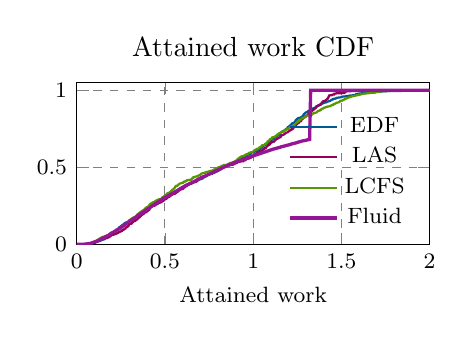
\begin{tikzpicture}
    \begin{axis}[
    title=Attained work CDF,
    width=0.5\textwidth,
    height=0.3\textwidth,
    xlabel={Attained work},
    xmin=0,xmax=2.0,
    ymin=0,ymax=1.05,
    grid,
    legend pos=south east,
    ]
    \addplot[color=azulcito, solid, thick]
        table[row sep={\\}]
        {
            \\
            0.048736832358898  0.0012484394506866417  \\
            0.06568419181435559  0.0024968789013732834  \\
            0.06784781055232614  0.003745318352059925  \\
            0.07499541434988544  0.004993757802746567  \\
            0.07585485918761492  0.006242197253433208  \\
            0.08208911866199742  0.00749063670411985  \\
            0.09690530397511375  0.008739076154806492  \\
            0.10288897082759263  0.009987515605493134  \\
            0.10440251914700024  0.011235955056179775  \\
            0.10525513633967432  0.012484394506866416  \\
            0.10690827337832332  0.01373283395755306  \\
            0.10965149888851045  0.0149812734082397  \\
            0.11357552085499378  0.016229712858926344  \\
            0.11394731975218875  0.017478152309612985  \\
            0.11957476794836452  0.018726591760299626  \\
            0.12249931072737312  0.019975031210986267  \\
            0.12416950366284141  0.02122347066167291  \\
            0.12950572378473169  0.02247191011235955  \\
            0.13335260129860166  0.02372034956304619  \\
            0.1368597164485151  0.024968789013732832  \\
            0.1396838769750265  0.026217228464419477  \\
            0.14225529994019107  0.02746566791510612  \\
            0.14514992789054823  0.02871410736579276  \\
            0.14536873173290132  0.0299625468164794  \\
            0.14578246532920502  0.031210986267166042  \\
            0.15488684387655025  0.03245942571785269  \\
            0.1568749406769231  0.033707865168539325  \\
            0.15843000343141966  0.03495630461922597  \\
            0.16053202494523858  0.03620474406991261  \\
            0.16167562793381762  0.03745318352059925  \\
            0.16207411914075465  0.03870162297128589  \\
            0.16416635342463098  0.039950062421972535  \\
            0.17119410973834012  0.04119850187265917  \\
            0.17230407329895028  0.04244694132334582  \\
            0.17305660806137269  0.04369538077403246  \\
            0.17318349954476275  0.0449438202247191  \\
            0.17340189608867007  0.046192259675405745  \\
            0.1744560024884311  0.04744069912609238  \\
            0.17483096449488025  0.04868913857677903  \\
            0.17657009827283332  0.049937578027465665  \\
            0.17700435908651216  0.05118601747815231  \\
            0.17849292349070112  0.052434456928838954  \\
            0.18031849554115809  0.05368289637952559  \\
            0.18042052208480808  0.05493133583021224  \\
            0.18141188318835463  0.056179775280898875  \\
            0.18169462583213422  0.05742821473158552  \\
            0.1827630008719261  0.05867665418227216  \\
            0.18299327264005644  0.0599250936329588  \\
            0.18479127956068875  0.06117353308364544  \\
            0.18589934553815143  0.062421972534332085  \\
            0.18642332590953767  0.06367041198501873  \\
            0.1919134663329487  0.06491885143570537  \\
            0.19400579850849478  0.066167290886392  \\
            0.1954575539009156  0.06741573033707865  \\
            0.196504035090317  0.0686641697877653  \\
            0.19991077641086036  0.06991260923845194  \\
            0.20036450180155532  0.07116104868913857  \\
            0.20153634022522116  0.07240948813982521  \\
            0.20173136194991065  0.07365792759051186  \\
            0.2026771853083815  0.0749063670411985  \\
            0.2059110533302259  0.07615480649188515  \\
            0.2060771976241342  0.07740324594257178  \\
            0.20757245689881318  0.07865168539325842  \\
            0.2087579021993804  0.07990012484394507  \\
            0.21003222332573995  0.08114856429463171  \\
            0.2135287493165805  0.08239700374531835  \\
            0.2144710972648352  0.08364544319600499  \\
            0.21485860574264848  0.08489388264669163  \\
            0.21687739537689288  0.08614232209737828  \\
            0.21694932905086078  0.08739076154806492  \\
            0.2179512580751484  0.08863920099875156  \\
            0.21940697838424025  0.0898876404494382  \\
            0.22127378352049826  0.09113607990012484  \\
            0.22442906525776607  0.09238451935081149  \\
            0.2246386366185669  0.09363295880149813  \\
            0.22491825937870913  0.09488139825218476  \\
            0.22804522079002018  0.09612983770287141  \\
            0.2304732969054939  0.09737827715355805  \\
            0.23102930363558016  0.0986267166042447  \\
            0.23269828623799815  0.09987515605493133  \\
            0.23580562566635876  0.10112359550561797  \\
            0.23580644292820807  0.10237203495630462  \\
            0.23690634863769808  0.10362047440699126  \\
            0.23734271937544799  0.10486891385767791  \\
            0.23785646598178226  0.10611735330836454  \\
            0.23813866503601844  0.10736579275905118  \\
            0.23882664353669725  0.10861423220973783  \\
            0.23894222190337408  0.10986267166042447  \\
            0.24110128482954002  0.1111111111111111  \\
            0.2429936830044832  0.11235955056179775  \\
            0.24550130069864906  0.1136079900124844  \\
            0.2467445642063808  0.11485642946317104  \\
            0.24819218918690922  0.11610486891385768  \\
            0.2510323769323948  0.11735330836454431  \\
            0.25154447171358685  0.11860174781523096  \\
            0.25208677920476674  0.1198501872659176  \\
            0.2537356136029232  0.12109862671660425  \\
            0.2548853054642012  0.12234706616729088  \\
            0.256174837627391  0.12359550561797752  \\
            0.2593941402721517  0.12484394506866417  \\
            0.2601497732656384  0.12609238451935081  \\
            0.26237666003416393  0.12734082397003746  \\
            0.2633063386159571  0.1285892634207241  \\
            0.2652706044851369  0.12983770287141075  \\
            0.2668444769716274  0.13108614232209737  \\
            0.2669184132722364  0.132334581772784  \\
            0.2701017925075652  0.13358302122347065  \\
            0.27114475523808523  0.1348314606741573  \\
            0.2714575348121193  0.13607990012484394  \\
            0.27168188632411394  0.1373283395755306  \\
            0.2723364604263736  0.13857677902621723  \\
            0.2744620527845859  0.13982521847690388  \\
            0.2759115408439257  0.14107365792759052  \\
            0.2814151639193199  0.14232209737827714  \\
            0.28610849191121  0.14357053682896379  \\
            0.28789314471518423  0.14481897627965043  \\
            0.2881178904938153  0.14606741573033707  \\
            0.2920186366615983  0.14731585518102372  \\
            0.2931555495876381  0.14856429463171036  \\
            0.2995964301933479  0.149812734082397  \\
            0.3027897797534783  0.15106117353308365  \\
            0.3051352388293296  0.1523096129837703  \\
            0.30578335470657847  0.15355805243445692  \\
            0.30644362249824625  0.15480649188514356  \\
            0.3072526782322456  0.1560549313358302  \\
            0.3091197200701714  0.15730337078651685  \\
            0.31189236545304055  0.1585518102372035  \\
            0.31282367428263674  0.15980024968789014  \\
            0.31288271563300896  0.16104868913857678  \\
            0.31368484352129855  0.16229712858926343  \\
            0.3158257597338975  0.16354556803995007  \\
            0.31756060943239106  0.1647940074906367  \\
            0.31765363693475024  0.16604244694132334  \\
            0.3199871797320881  0.16729088639200998  \\
            0.3207868141623971  0.16853932584269662  \\
            0.32130319239889427  0.16978776529338327  \\
            0.32534123674662135  0.17103620474406991  \\
            0.32540250221187256  0.17228464419475656  \\
            0.3266670494822233  0.1735330836454432  \\
            0.3299643856954475  0.17478152309612985  \\
            0.33150371973866954  0.1760299625468165  \\
            0.33177376713947015  0.1772784019975031  \\
            0.33403260815759944  0.17852684144818975  \\
            0.33616187824852517  0.1797752808988764  \\
            0.3366104183748384  0.18102372034956304  \\
            0.336678943911224  0.1822721598002497  \\
            0.33679108405388547  0.18352059925093633  \\
            0.33698065939642846  0.18476903870162298  \\
            0.33864853766703373  0.18601747815230962  \\
            0.3416479799615676  0.18726591760299627  \\
            0.3465835489863879  0.18851435705368288  \\
            0.34784285182473695  0.18976279650436953  \\
            0.35001649972879534  0.19101123595505617  \\
            0.3530029793957428  0.19225967540574282  \\
            0.3545430786970627  0.19350811485642946  \\
            0.35729588325898476  0.1947565543071161  \\
            0.35764886960839704  0.19600499375780275  \\
            0.35915097569659693  0.1972534332084894  \\
            0.3610711307715252  0.19850187265917604  \\
            0.3633604389739844  0.19975031210986266  \\
            0.3659277216403325  0.2009987515605493  \\
            0.36956643552134594  0.20224719101123595  \\
            0.3698914967278171  0.2034956304619226  \\
            0.37055336701157415  0.20474406991260924  \\
            0.3710859572786346  0.20599250936329588  \\
            0.3711974112447365  0.20724094881398253  \\
            0.37162806805164644  0.20848938826466917  \\
            0.3723305489756929  0.20973782771535582  \\
            0.37257541831815644  0.21098626716604243  \\
            0.3771479328572412  0.21223470661672908  \\
            0.3787188186355195  0.21348314606741572  \\
            0.38066993255119996  0.21473158551810237  \\
            0.38266891470699194  0.21598002496878901  \\
            0.38269572242498917  0.21722846441947566  \\
            0.3838825254714021  0.2184769038701623  \\
            0.3840325857236565  0.21972534332084895  \\
            0.38528056990244863  0.2209737827715356  \\
            0.3862876483220319  0.2222222222222222  \\
            0.3871920030607008  0.22347066167290885  \\
            0.38795223289862896  0.2247191011235955  \\
            0.3918728100146893  0.22596754057428214  \\
            0.3919739261908059  0.2272159800249688  \\
            0.39288986762647937  0.22846441947565543  \\
            0.3940221473272886  0.22971285892634208  \\
            0.39578403170070675  0.23096129837702872  \\
            0.3989643078765891  0.23220973782771537  \\
            0.39916197204927223  0.23345817727840198  \\
            0.39977045396160804  0.23470661672908863  \\
            0.4027236606429841  0.23595505617977527  \\
            0.4031328794687471  0.23720349563046192  \\
            0.40984980917126584  0.23845193508114856  \\
            0.41009916658259016  0.2397003745318352  \\
            0.41057456302118245  0.24094881398252185  \\
            0.41100169220098337  0.2421972534332085  \\
            0.4122140071328033  0.24344569288389514  \\
            0.4146163005543542  0.24469413233458176  \\
            0.41500872704047964  0.2459425717852684  \\
            0.4153646359697234  0.24719101123595505  \\
            0.4158305853230857  0.2484394506866417  \\
            0.4159579512931787  0.24968789013732834  \\
            0.4176283066060891  0.250936329588015  \\
            0.41948498223751224  0.25218476903870163  \\
            0.42191415031267354  0.2534332084893883  \\
            0.4220865367260126  0.2546816479400749  \\
            0.4254561394133418  0.25593008739076156  \\
            0.42573636230092404  0.2571785268414482  \\
            0.4274167353545937  0.25842696629213485  \\
            0.43093741272824104  0.2596754057428215  \\
            0.43613436385449317  0.26092384519350814  \\
            0.44158208987884257  0.26217228464419473  \\
            0.44169808812285916  0.2634207240948814  \\
            0.4423764631126661  0.264669163545568  \\
            0.44456977223825345  0.26591760299625467  \\
            0.4467379617050825  0.2671660424469413  \\
            0.44803058304879073  0.26841448189762795  \\
            0.4536432016838318  0.2696629213483146  \\
            0.45539426717164644  0.27091136079900124  \\
            0.4588895490227003  0.2721598002496879  \\
            0.46120923402482095  0.27340823970037453  \\
            0.4654815590502924  0.2746566791510612  \\
            0.4661286862134353  0.2759051186017478  \\
            0.4676047392463545  0.27715355805243447  \\
            0.46790412862915787  0.2784019975031211  \\
            0.46887001156403585  0.27965043695380776  \\
            0.47108338161968943  0.2808988764044944  \\
            0.47128675221915717  0.28214731585518105  \\
            0.47412450200670264  0.2833957553058677  \\
            0.4755545245004243  0.2846441947565543  \\
            0.4773943745529565  0.2858926342072409  \\
            0.4784486375096871  0.28714107365792757  \\
            0.47973793412228527  0.2883895131086142  \\
            0.4799744051487522  0.28963795255930086  \\
            0.4807253045176906  0.2908863920099875  \\
            0.48077189977345935  0.29213483146067415  \\
            0.4829072490624534  0.2933832709113608  \\
            0.4842620899146944  0.29463171036204744  \\
            0.4844104296126282  0.2958801498127341  \\
            0.48447480504662344  0.29712858926342073  \\
            0.4888418578968036  0.2983770287141074  \\
            0.4902544965934936  0.299625468164794  \\
            0.4908460288720988  0.30087390761548066  \\
            0.49606674138332874  0.3021223470661673  \\
            0.4968494353775213  0.30337078651685395  \\
            0.5008409169549193  0.3046192259675406  \\
            0.5010681457411295  0.30586766541822724  \\
            0.502578194964596  0.30711610486891383  \\
            0.5043172949900466  0.3083645443196005  \\
            0.505895920251901  0.3096129837702871  \\
            0.5095198514454613  0.31086142322097376  \\
            0.5131987285437987  0.3121098626716604  \\
            0.51403718005011  0.31335830212234705  \\
            0.5257274241331622  0.3146067415730337  \\
            0.5264121593992876  0.31585518102372034  \\
            0.5268449961373562  0.317103620474407  \\
            0.5297633302293148  0.31835205992509363  \\
            0.5299819584489854  0.3196004993757803  \\
            0.5326282410884318  0.3208489388264669  \\
            0.5335978132592063  0.32209737827715357  \\
            0.5382490106446838  0.3233458177278402  \\
            0.54044605929513  0.32459425717852686  \\
            0.5416099068392626  0.3258426966292135  \\
            0.5443032482733572  0.32709113607990015  \\
            0.5503255817415318  0.3283395755305868  \\
            0.5532877021456954  0.3295880149812734  \\
            0.553731908500495  0.33083645443196  \\
            0.5548242677393489  0.33208489388264667  \\
            0.5573156115406556  0.3333333333333333  \\
            0.5580702698359088  0.33458177278401996  \\
            0.5580733003308893  0.3358302122347066  \\
            0.5586427940356335  0.33707865168539325  \\
            0.5603318699633668  0.3383270911360799  \\
            0.561041502837867  0.33957553058676654  \\
            0.5637162008047841  0.3408239700374532  \\
            0.5661163964804254  0.34207240948813983  \\
            0.5665710815470746  0.3433208489388265  \\
            0.5693828204288747  0.3445692883895131  \\
            0.5706518759568904  0.34581772784019976  \\
            0.5714663137402951  0.3470661672908864  \\
            0.5717408585275339  0.34831460674157305  \\
            0.5728285263869138  0.3495630461922597  \\
            0.5737326040617147  0.35081148564294634  \\
            0.5743825921795324  0.352059925093633  \\
            0.5755458620424818  0.3533083645443196  \\
            0.576538194582831  0.3545568039950062  \\
            0.5767787531117536  0.35580524344569286  \\
            0.5788052208426568  0.3570536828963795  \\
            0.5810028915515971  0.35830212234706615  \\
            0.581989312309372  0.3595505617977528  \\
            0.582318059560212  0.36079900124843944  \\
            0.584023934801969  0.3620474406991261  \\
            0.5847467157172197  0.36329588014981273  \\
            0.5880473609571547  0.3645443196004994  \\
            0.5964982725869761  0.365792759051186  \\
            0.5965259810970301  0.36704119850187267  \\
            0.5995091805071269  0.3682896379525593  \\
            0.6025979792726105  0.36953807740324596  \\
            0.603032585471054  0.3707865168539326  \\
            0.6054406753911081  0.37203495630461925  \\
            0.6073656489607706  0.3732833957553059  \\
            0.6119194690249923  0.37453183520599254  \\
            0.614643913320042  0.3757802746566791  \\
            0.6209188903637326  0.37702871410736577  \\
            0.6209721359082037  0.3782771535580524  \\
            0.6212055570684561  0.37952559300873906  \\
            0.6231693438410857  0.3807740324594257  \\
            0.6233031048286195  0.38202247191011235  \\
            0.6273828005761966  0.383270911360799  \\
            0.628678183087974  0.38451935081148564  \\
            0.6286789444938761  0.3857677902621723  \\
            0.6299541134702996  0.38701622971285893  \\
            0.6304896054188589  0.3882646691635456  \\
            0.633845913481902  0.3895131086142322  \\
            0.6349865173637093  0.39076154806491886  \\
            0.6372383625907787  0.3920099875156055  \\
            0.6400537966763835  0.39325842696629215  \\
            0.6416682316913691  0.3945068664169788  \\
            0.646911763339677  0.39575530586766544  \\
            0.651070402853048  0.3970037453183521  \\
            0.6522151782675847  0.3982521847690387  \\
            0.6544893468134203  0.3995006242197253  \\
            0.658899545768869  0.40074906367041196  \\
            0.6605287961511372  0.4019975031210986  \\
            0.6643558449919559  0.40324594257178525  \\
            0.6651507408017165  0.4044943820224719  \\
            0.6655553273745081  0.40574282147315854  \\
            0.6677290481899806  0.4069912609238452  \\
            0.6731999667447326  0.40823970037453183  \\
            0.6785584702389847  0.4094881398252185  \\
            0.6808844136515972  0.4107365792759051  \\
            0.6825447128943268  0.41198501872659177  \\
            0.6828549903295311  0.4132334581772784  \\
            0.6851378943568704  0.41448189762796506  \\
            0.685968933565718  0.4157303370786517  \\
            0.6886876622435807  0.41697877652933835  \\
            0.6893917258727386  0.418227215980025  \\
            0.6909372531618205  0.41947565543071164  \\
            0.6917380798984921  0.4207240948813982  \\
            0.7011675810742943  0.42197253433208487  \\
            0.7057721563058625  0.4232209737827715  \\
            0.7065181783399552  0.42446941323345816  \\
            0.709355995143423  0.4257178526841448  \\
            0.7137383561081463  0.42696629213483145  \\
            0.7145066683494931  0.4282147315855181  \\
            0.7146032241915208  0.42946317103620474  \\
            0.7155762470177294  0.4307116104868914  \\
            0.7163080716042716  0.43196004993757803  \\
            0.7187072313335533  0.4332084893882647  \\
            0.720939251032874  0.4344569288389513  \\
            0.7244765609479203  0.43570536828963796  \\
            0.7261348537292635  0.4369538077403246  \\
            0.7280919969769035  0.43820224719101125  \\
            0.7287216482916237  0.4394506866416979  \\
            0.7302329909214199  0.44069912609238454  \\
            0.7328029372328582  0.4419475655430712  \\
            0.7335922028850916  0.4431960049937578  \\
            0.7359042907403626  0.4444444444444444  \\
            0.7367111004211991  0.44569288389513106  \\
            0.7386242589167015  0.4469413233458177  \\
            0.7409845053818309  0.44818976279650435  \\
            0.7427154003664223  0.449438202247191  \\
            0.7464590287983837  0.45068664169787764  \\
            0.7470266476220216  0.4519350811485643  \\
            0.7491515890002913  0.45318352059925093  \\
            0.7504480843829524  0.4544319600499376  \\
            0.7551158662662829  0.4556803995006242  \\
            0.7560257491063709  0.45692883895131087  \\
            0.7662800910235608  0.4581772784019975  \\
            0.766514553186681  0.45942571785268416  \\
            0.7690341439586011  0.4606741573033708  \\
            0.7699015731063305  0.46192259675405745  \\
            0.7769566801089578  0.4631710362047441  \\
            0.778810370157071  0.46441947565543074  \\
            0.7797584305985481  0.4656679151061174  \\
            0.7827395150403114  0.46691635455680397  \\
            0.7850350736956848  0.4681647940074906  \\
            0.7858128320759918  0.46941323345817726  \\
            0.7865959925793223  0.4706616729088639  \\
            0.7911749730663867  0.47191011235955055  \\
            0.7962417046956923  0.4731585518102372  \\
            0.7964513228842236  0.47440699126092384  \\
            0.7986933594449154  0.4756554307116105  \\
            0.8004281817724603  0.4769038701622971  \\
            0.8037540844280359  0.4781523096129838  \\
            0.8049966111621009  0.4794007490636704  \\
            0.8063733065495793  0.48064918851435706  \\
            0.8072315391642845  0.4818976279650437  \\
            0.8093021857889653  0.48314606741573035  \\
            0.8096103767657046  0.484394506866417  \\
            0.8101168477364096  0.48564294631710364  \\
            0.8173150597764587  0.4868913857677903  \\
            0.8187041792056193  0.48813982521847693  \\
            0.8192288203846743  0.4893882646691635  \\
            0.8203945296814936  0.49063670411985016  \\
            0.8208327972910469  0.4918851435705368  \\
            0.8209537909163992  0.49313358302122345  \\
            0.8221474206293949  0.4943820224719101  \\
            0.8229245251746844  0.49563046192259674  \\
            0.8229513148627063  0.4968789013732834  \\
            0.8230023267417436  0.49812734082397003  \\
            0.8280529921845634  0.4993757802746567  \\
            0.8319981781508261  0.5006242197253433  \\
            0.8327112415815691  0.50187265917603  \\
            0.833341345569778  0.5031210986267166  \\
            0.8348432045094967  0.5043695380774033  \\
            0.8351836171731506  0.5056179775280899  \\
            0.8383678264737409  0.5068664169787765  \\
            0.8433079547118183  0.5081148564294632  \\
            0.8505149556093841  0.5093632958801498  \\
            0.8505395104429568  0.5106117353308365  \\
            0.851818237052005  0.5118601747815231  \\
            0.8528888178373031  0.5131086142322098  \\
            0.8571105564742879  0.5143570536828964  \\
            0.8601484721553394  0.5156054931335831  \\
            0.8617907511305494  0.5168539325842697  \\
            0.8632274932232917  0.5181023720349563  \\
            0.8654622758380555  0.519350811485643  \\
            0.8678935873458142  0.5205992509363296  \\
            0.8680819697406363  0.5218476903870163  \\
            0.8707181419757148  0.5230961298377028  \\
            0.8722095492595656  0.5243445692883895  \\
            0.8730097323201487  0.5255930087390761  \\
            0.8758421926531099  0.5268414481897628  \\
            0.8815935800522312  0.5280898876404494  \\
            0.8860645232723491  0.529338327091136  \\
            0.8867414108797118  0.5305867665418227  \\
            0.8886830990447405  0.5318352059925093  \\
            0.8898263028566199  0.533083645443196  \\
            0.8969463068065759  0.5343320848938826  \\
            0.8990792682337345  0.5355805243445693  \\
            0.9027343006571584  0.5368289637952559  \\
            0.9047497518359507  0.5380774032459426  \\
            0.9062356631270083  0.5393258426966292  \\
            0.9083346831885991  0.5405742821473158  \\
            0.9097440823334041  0.5418227215980025  \\
            0.9102975731175036  0.5430711610486891  \\
            0.9119420100536784  0.5443196004993758  \\
            0.9189909061365259  0.5455680399500624  \\
            0.9217763632549776  0.5468164794007491  \\
            0.9220017241163108  0.5480649188514357  \\
            0.9248405468448133  0.5493133583021224  \\
            0.925496525261297  0.550561797752809  \\
            0.9285270089290669  0.5518102372034956  \\
            0.9294229800492244  0.5530586766541823  \\
            0.9315819296157715  0.5543071161048689  \\
            0.9322675234931261  0.5555555555555556  \\
            0.9343945413212673  0.5568039950062422  \\
            0.9356969680084926  0.5580524344569289  \\
            0.9373449095780533  0.5593008739076155  \\
            0.9398532940857076  0.5605493133583022  \\
            0.9430620824080189  0.5617977528089888  \\
            0.9435052912587849  0.5630461922596754  \\
            0.945421490116843  0.5642946317103621  \\
            0.9482493659760676  0.5655430711610487  \\
            0.9526108022408932  0.5667915106117354  \\
            0.9546267763393406  0.568039950062422  \\
            0.9570238109548683  0.5692883895131086  \\
            0.9572982187324426  0.5705368289637952  \\
            0.9597207130719316  0.5717852684144819  \\
            0.9602353804761774  0.5730337078651685  \\
            0.9621120531740444  0.5742821473158551  \\
            0.9659799733113488  0.5755305867665418  \\
            0.9678096342619826  0.5767790262172284  \\
            0.9684147302032784  0.5780274656679151  \\
            0.9685787419870353  0.5792759051186017  \\
            0.9688086312522463  0.5805243445692884  \\
            0.9689694700147622  0.581772784019975  \\
            0.9694401050557531  0.5830212234706617  \\
            0.977114248245134  0.5842696629213483  \\
            0.9825383138251964  0.5855181023720349  \\
            0.9851981648707091  0.5867665418227216  \\
            0.9871428405864506  0.5880149812734082  \\
            0.9882496246897405  0.5892634207240949  \\
            0.9887479295104877  0.5905118601747815  \\
            0.9890818960506376  0.5917602996254682  \\
            0.9896311907220916  0.5930087390761548  \\
            0.9897620741367992  0.5942571785268415  \\
            0.992472855701074  0.5955056179775281  \\
            0.9945543734086839  0.5967540574282147  \\
            1.001435085661389  0.5980024968789014  \\
            1.0036949271278637  0.599250936329588  \\
            1.0054489841270582  0.6004993757802747  \\
            1.0098094160676823  0.6017478152309613  \\
            1.0101037807116313  0.602996254681648  \\
            1.0134263948789966  0.6042446941323346  \\
            1.0145619913485402  0.6054931335830213  \\
            1.0198733700373426  0.6067415730337079  \\
            1.0203388078045335  0.6079900124843945  \\
            1.0261523399122439  0.6092384519350812  \\
            1.026198296370755  0.6104868913857678  \\
            1.03256354270998  0.6117353308364545  \\
            1.0355367708309506  0.6129837702871411  \\
            1.0368604565457389  0.6142322097378277  \\
            1.0374263667633266  0.6154806491885143  \\
            1.0382749488563536  0.616729088639201  \\
            1.0383166891817464  0.6179775280898876  \\
            1.040578971596481  0.6192259675405742  \\
            1.041923759782697  0.6204744069912609  \\
            1.041965516179237  0.6217228464419475  \\
            1.0423502959197637  0.6229712858926342  \\
            1.0454105844048587  0.6242197253433208  \\
            1.0481346620810126  0.6254681647940075  \\
            1.048288262709569  0.6267166042446941  \\
            1.0492980807702454  0.6279650436953808  \\
            1.0508510026594702  0.6292134831460674  \\
            1.051373254570339  0.630461922596754  \\
            1.052386384040538  0.6317103620474407  \\
            1.0528923968628119  0.6329588014981273  \\
            1.0562791768719282  0.634207240948814  \\
            1.056393202572757  0.6354556803995006  \\
            1.0578175630349782  0.6367041198501873  \\
            1.0582551135336749  0.6379525593008739  \\
            1.0585276087300306  0.6392009987515606  \\
            1.0612312891534388  0.6404494382022472  \\
            1.0620052263343502  0.6416978776529338  \\
            1.062195368363497  0.6429463171036205  \\
            1.0644816829168118  0.6441947565543071  \\
            1.0662275319752954  0.6454431960049938  \\
            1.0666232072751838  0.6466916354556804  \\
            1.067181130600197  0.6479400749063671  \\
            1.0673804729941734  0.6491885143570537  \\
            1.0677942933232603  0.6504369538077404  \\
            1.0737232128666139  0.651685393258427  \\
            1.080840185853274  0.6529338327091136  \\
            1.0821749855979237  0.6541822721598003  \\
            1.08477803406478  0.6554307116104869  \\
            1.0857902386850502  0.6566791510611736  \\
            1.088483008627863  0.6579275905118602  \\
            1.0936217398247052  0.6591760299625468  \\
            1.0936370035954002  0.6604244694132334  \\
            1.0937746377959796  0.66167290886392  \\
            1.093975586149752  0.6629213483146067  \\
            1.0959834201292142  0.6641697877652933  \\
            1.0976248338780576  0.66541822721598  \\
            1.0991690399693061  0.6666666666666666  \\
            1.0999530496480738  0.6679151061173533  \\
            1.1005055527047438  0.6691635455680399  \\
            1.1005752717222848  0.6704119850187266  \\
            1.1011005243843197  0.6716604244694132  \\
            1.1027139582820524  0.6729088639200999  \\
            1.103566743575148  0.6741573033707865  \\
            1.1047171581306916  0.6754057428214731  \\
            1.1058872833949258  0.6766541822721598  \\
            1.1063368184067386  0.6779026217228464  \\
            1.1085578149374344  0.6791510611735331  \\
            1.1092456783103728  0.6803995006242197  \\
            1.109418128654197  0.6816479400749064  \\
            1.1099163725715027  0.682896379525593  \\
            1.1115479978807494  0.6841448189762797  \\
            1.1122984985729256  0.6853932584269663  \\
            1.1148682646404002  0.686641697877653  \\
            1.1155790223209863  0.6878901373283396  \\
            1.116287190405448  0.6891385767790262  \\
            1.1170238396637582  0.6903870162297129  \\
            1.1202143482062912  0.6916354556803995  \\
            1.1203782633099664  0.6928838951310862  \\
            1.1204666041217037  0.6941323345817728  \\
            1.1235023061237261  0.6953807740324595  \\
            1.1290442777564749  0.6966292134831461  \\
            1.1301049903853198  0.6978776529338327  \\
            1.131383390257355  0.6991260923845194  \\
            1.1327953917960385  0.700374531835206  \\
            1.136456639501929  0.7016229712858927  \\
            1.1372455379825865  0.7028714107365793  \\
            1.137733447076483  0.704119850187266  \\
            1.139243266382541  0.7053682896379525  \\
            1.1430450643194745  0.7066167290886392  \\
            1.143770834024821  0.7078651685393258  \\
            1.1440096716927082  0.7091136079900124  \\
            1.1453761737974912  0.7103620474406991  \\
            1.145452401229477  0.7116104868913857  \\
            1.1455164474716115  0.7128589263420724  \\
            1.1458397698034968  0.714107365792759  \\
            1.1467277745027786  0.7153558052434457  \\
            1.1529567985060396  0.7166042446941323  \\
            1.153352841619224  0.717852684144819  \\
            1.1537243805569082  0.7191011235955056  \\
            1.1540824357937847  0.7203495630461922  \\
            1.1545306507028248  0.7215980024968789  \\
            1.1546411828545757  0.7228464419475655  \\
            1.1558138076086935  0.7240948813982522  \\
            1.1569967603140296  0.7253433208489388  \\
            1.159464570720287  0.7265917602996255  \\
            1.1614062895874608  0.7278401997503121  \\
            1.1617204904435865  0.7290886392009988  \\
            1.1628333378177675  0.7303370786516854  \\
            1.1636766687065478  0.731585518102372  \\
            1.164587871426995  0.7328339575530587  \\
            1.1691851506989392  0.7340823970037453  \\
            1.1695650603411298  0.735330836454432  \\
            1.171712011562013  0.7365792759051186  \\
            1.1762069813735607  0.7378277153558053  \\
            1.1785444203599909  0.7390761548064919  \\
            1.1805152007413788  0.7403245942571786  \\
            1.1811286803356609  0.7415730337078652  \\
            1.1823973572790085  0.7428214731585518  \\
            1.1826898572643127  0.7440699126092385  \\
            1.1831511486301458  0.7453183520599251  \\
            1.1851901619621394  0.7465667915106118  \\
            1.186970818797394  0.7478152309612984  \\
            1.189213637523066  0.7490636704119851  \\
            1.1899778876703886  0.7503121098626716  \\
            1.1919292538774027  0.7515605493133583  \\
            1.193251164253014  0.7528089887640449  \\
            1.1938752414076852  0.7540574282147315  \\
            1.1951696918777799  0.7553058676654182  \\
            1.1958019435815084  0.7565543071161048  \\
            1.1960552373067792  0.7578027465667915  \\
            1.19627532237792  0.7590511860174781  \\
            1.1963664131485658  0.7602996254681648  \\
            1.199298087263759  0.7615480649188514  \\
            1.2035145864105772  0.762796504369538  \\
            1.2037972011235967  0.7640449438202247  \\
            1.203934358685792  0.7652933832709113  \\
            1.2058095336806787  0.766541822721598  \\
            1.2063745041638612  0.7677902621722846  \\
            1.2069989554149332  0.7690387016229713  \\
            1.2083043176781154  0.7702871410736579  \\
            1.210219097380702  0.7715355805243446  \\
            1.2108660105317508  0.7727840199750312  \\
            1.2135392364672972  0.7740324594257179  \\
            1.213722553728096  0.7752808988764045  \\
            1.213849991386724  0.7765293383270911  \\
            1.2152753471882825  0.7777777777777778  \\
            1.216653151948322  0.7790262172284644  \\
            1.2184979636707853  0.7802746566791511  \\
            1.2192844821075566  0.7815230961298377  \\
            1.2196216132049176  0.7827715355805244  \\
            1.2199063906796739  0.784019975031211  \\
            1.2227893279902462  0.7852684144818977  \\
            1.2277154068197038  0.7865168539325843  \\
            1.2300405345369967  0.787765293383271  \\
            1.2341960470955222  0.7890137328339576  \\
            1.2342563288861421  0.7902621722846442  \\
            1.2347291991278575  0.7915106117353309  \\
            1.2352669728715395  0.7927590511860175  \\
            1.2355148733981278  0.7940074906367042  \\
            1.2355421964742277  0.7952559300873908  \\
            1.2369180851585364  0.7965043695380774  \\
            1.2389757347158818  0.797752808988764  \\
            1.2392710442427526  0.7990012484394506  \\
            1.2403775113109374  0.8002496878901373  \\
            1.24071254431977  0.8014981273408239  \\
            1.2410222180026254  0.8027465667915106  \\
            1.2410260146395018  0.8039950062421972  \\
            1.2413865207153372  0.8052434456928839  \\
            1.2424253649284653  0.8064918851435705  \\
            1.2457908914161528  0.8077403245942572  \\
            1.2459148858557834  0.8089887640449438  \\
            1.2463077250810013  0.8102372034956304  \\
            1.2467016803103763  0.8114856429463171  \\
            1.2486959294571274  0.8127340823970037  \\
            1.250657274767618  0.8139825218476904  \\
            1.2526096026410463  0.815230961298377  \\
            1.2536354713676157  0.8164794007490637  \\
            1.2537014500642276  0.8177278401997503  \\
            1.2553707801178704  0.818976279650437  \\
            1.2622643667283349  0.8202247191011236  \\
            1.2650076971619812  0.8214731585518102  \\
            1.2703632622532028  0.8227215980024969  \\
            1.2713123190473221  0.8239700374531835  \\
            1.2718767551561008  0.8252184769038702  \\
            1.2744236149945611  0.8264669163545568  \\
            1.276674045751399  0.8277153558052435  \\
            1.2775318915828588  0.8289637952559301  \\
            1.2784030884811979  0.8302122347066168  \\
            1.2802760488634752  0.8314606741573034  \\
            1.2813746067313265  0.83270911360799  \\
            1.2819121404147065  0.8339575530586767  \\
            1.2833758202639565  0.8352059925093633  \\
            1.2839304677663497  0.83645443196005  \\
            1.284135116865449  0.8377028714107366  \\
            1.2848366973625582  0.8389513108614233  \\
            1.2855458675831244  0.8401997503121099  \\
            1.2857451130424837  0.8414481897627965  \\
            1.287260323434171  0.8426966292134831  \\
            1.288426544188439  0.8439450686641697  \\
            1.2893949433546064  0.8451935081148564  \\
            1.2896121738588866  0.846441947565543  \\
            1.2919638062369927  0.8476903870162297  \\
            1.2932103535229993  0.8489388264669163  \\
            1.293376982386708  0.850187265917603  \\
            1.2950072788099205  0.8514357053682896  \\
            1.2960250129863038  0.8526841448189763  \\
            1.2975413100843545  0.8539325842696629  \\
            1.2979424079699469  0.8551810237203495  \\
            1.3006710307385483  0.8564294631710362  \\
            1.301949671589834  0.8576779026217228  \\
            1.3080159333579664  0.8589263420724095  \\
            1.3087424313677891  0.8601747815230961  \\
            1.3101461704625175  0.8614232209737828  \\
            1.310330983076492  0.8626716604244694  \\
            1.3108152616192967  0.8639200998751561  \\
            1.3115793235019124  0.8651685393258427  \\
            1.3152469243601272  0.8664169787765293  \\
            1.3184403685045165  0.867665418227216  \\
            1.319205813564654  0.8689138576779026  \\
            1.3203777395619727  0.8701622971285893  \\
            1.3222262423683473  0.8714107365792759  \\
            1.3241532485384373  0.8726591760299626  \\
            1.3269941316141938  0.8739076154806492  \\
            1.328882344561972  0.8751560549313359  \\
            1.330101382161848  0.8764044943820225  \\
            1.3337970262225638  0.8776529338327091  \\
            1.3357217920169746  0.8789013732833958  \\
            1.3357871994094888  0.8801498127340824  \\
            1.338351515825074  0.8813982521847691  \\
            1.3406488003881532  0.8826466916354557  \\
            1.3437025728036849  0.8838951310861424  \\
            1.3456433337926001  0.885143570536829  \\
            1.3471312331700607  0.8863920099875156  \\
            1.3545366759093977  0.8876404494382022  \\
            1.3546696505636069  0.8888888888888888  \\
            1.355278709767816  0.8901373283395755  \\
            1.357028270003852  0.8913857677902621  \\
            1.358784388224425  0.8926342072409488  \\
            1.359715229383106  0.8938826466916354  \\
            1.3614319162232242  0.8951310861423221  \\
            1.3631326620116804  0.8963795255930087  \\
            1.3637181169988533  0.8976279650436954  \\
            1.3656391632455205  0.898876404494382  \\
            1.3694726494150924  0.9001248439450686  \\
            1.3697130358925245  0.9013732833957553  \\
            1.371518794801501  0.9026217228464419  \\
            1.3748838172343785  0.9038701622971286  \\
            1.3786843028604139  0.9051186017478152  \\
            1.3789559811994874  0.9063670411985019  \\
            1.3812554614757317  0.9076154806491885  \\
            1.3813719413761167  0.9088639200998752  \\
            1.3854084598272678  0.9101123595505618  \\
            1.3854935123587517  0.9113607990012484  \\
            1.3878352467107362  0.9126092384519351  \\
            1.3945792797342618  0.9138576779026217  \\
            1.3950016067931845  0.9151061173533084  \\
            1.3960315767453668  0.916354556803995  \\
            1.3993404913137546  0.9176029962546817  \\
            1.4043783269429977  0.9188514357053683  \\
            1.4096980072509349  0.920099875156055  \\
            1.4140957867012842  0.9213483146067416  \\
            1.414194079838051  0.9225967540574282  \\
            1.417871759908165  0.9238451935081149  \\
            1.4196573376964219  0.9250936329588015  \\
            1.4225556494829474  0.9263420724094882  \\
            1.4271177885171227  0.9275905118601748  \\
            1.4314193543607758  0.9288389513108615  \\
            1.4344583779788946  0.9300873907615481  \\
            1.436763249623782  0.9313358302122348  \\
            1.4382555141855362  0.9325842696629213  \\
            1.4390427395313043  0.9338327091136079  \\
            1.440707219561885  0.9350811485642946  \\
            1.4427577857083378  0.9363295880149812  \\
            1.4453627850988373  0.9375780274656679  \\
            1.4470127132626005  0.9388264669163545  \\
            1.4512324138630677  0.9400749063670412  \\
            1.451235733755103  0.9413233458177278  \\
            1.4557697662799414  0.9425717852684145  \\
            1.45762799083168  0.9438202247191011  \\
            1.4650409475007646  0.9450686641697877  \\
            1.465398982248466  0.9463171036204744  \\
            1.4701463155436905  0.947565543071161  \\
            1.4735390778622575  0.9488139825218477  \\
            1.4738066495419564  0.9500624219725343  \\
            1.4770013846289989  0.951310861423221  \\
            1.48739480411097  0.9525593008739076  \\
            1.4956504469015037  0.9538077403245943  \\
            1.4995252426780894  0.9550561797752809  \\
            1.5021593838084923  0.9563046192259675  \\
            1.5022260491385544  0.9575530586766542  \\
            1.5087167834549025  0.9588014981273408  \\
            1.5224755585073142  0.9600499375780275  \\
            1.5255428024119624  0.9612983770287141  \\
            1.5334412702804963  0.9625468164794008  \\
            1.5437025376283486  0.9637952559300874  \\
            1.546767310081532  0.9650436953807741  \\
            1.5622315503831716  0.9662921348314607  \\
            1.5637619062710446  0.9675405742821473  \\
            1.5705595593658543  0.968789013732834  \\
            1.578746297457386  0.9700374531835206  \\
            1.5799423987658179  0.9712858926342073  \\
            1.5816355451142776  0.9725343320848939  \\
            1.5822888699056668  0.9737827715355806  \\
            1.584226182679408  0.9750312109862672  \\
            1.5898452079402328  0.9762796504369539  \\
            1.5911942640180077  0.9775280898876404  \\
            1.610791781230633  0.978776529338327  \\
            1.613351630034211  0.9800249687890137  \\
            1.6378783232940655  0.9812734082397003  \\
            1.6427007811899537  0.982521847690387  \\
            1.6740215241111847  0.9837702871410736  \\
            1.67921611579776  0.9850187265917603  \\
            1.6854673998734833  0.9862671660424469  \\
            1.6873526132197176  0.9875156054931336  \\
            1.7075211465931042  0.9887640449438202  \\
            1.710655555301288  0.9900124843945068  \\
            1.7280276683098814  0.9912609238451935  \\
            1.7340055002537325  0.9925093632958801  \\
            1.7493378066738203  0.9937578027465668  \\
            1.826747849661354  0.9950062421972534  \\
            1.862011427068384  0.9962546816479401  \\
            1.8796397014115422  0.9975031210986267  \\
            1.8926768370726985  0.9987515605493134  \\
            1.964785621594955  1.0  \\
        }
        ;
    \addlegendentry {EDF}
    \addplot[color=rojito, solid, thick]
        table[row sep={\\}]
        {
            \\
                        0.016509288868315066  0.0012484394506866417  \\
            0.06156879759629419  0.0024968789013732834  \\
            0.07585485918761492  0.003745318352059925  \\
            0.08603125280968243  0.004993757802746567  \\
            0.0870161587340732  0.006242197253433208  \\
            0.09185349285667144  0.00749063670411985  \\
            0.09282372550313109  0.008739076154806492  \\
            0.09532058277735923  0.009987515605493134  \\
            0.09541433314547024  0.011235955056179775  \\
            0.10374155033622401  0.012484394506866416  \\
            0.10525513633967432  0.01373283395755306  \\
            0.10800147257506867  0.0149812734082397  \\
            0.11161937437675107  0.016229712858926344  \\
            0.11449014135192215  0.017478152309612985  \\
            0.11583829005978372  0.018726591760299626  \\
            0.11973588806293378  0.019975031210986267  \\
            0.12514421487207983  0.02122347066167291  \\
            0.12548797475496085  0.02247191011235955  \\
            0.127183954387867  0.02372034956304619  \\
            0.13067800635865487  0.024968789013732832  \\
            0.1311917360829895  0.026217228464419477  \\
            0.1319503746864683  0.02746566791510612  \\
            0.13230482303917768  0.02871410736579276  \\
            0.13376983822430333  0.0299625468164794  \\
            0.1345472895959482  0.031210986267166042  \\
            0.13616564122244768  0.03245942571785269  \\
            0.1383858622923839  0.033707865168539325  \\
            0.1402041631304769  0.03495630461922597  \\
            0.1405079790121274  0.03620474406991261  \\
            0.14177163726175185  0.03745318352059925  \\
            0.1447276191686046  0.03870162297128589  \\
            0.1525308530921663  0.039950062421972535  \\
            0.17119410973834012  0.04119850187265917  \\
            0.17216316381049168  0.04244694132334582  \\
            0.17574837496963974  0.04369538077403246  \\
            0.17629050402579338  0.0449438202247191  \\
            0.18173070107874523  0.046192259675405745  \\
            0.18382974650649314  0.04744069912609238  \\
            0.18580277570396558  0.04868913857677903  \\
            0.1858090717663714  0.049937578027465665  \\
            0.18633649433128316  0.05118601747815231  \\
            0.18743116337907395  0.052434456928838954  \\
            0.1878261374516601  0.05368289637952559  \\
            0.19278756180599457  0.05493133583021224  \\
            0.19400579850849478  0.056179775280898875  \\
            0.1946677615046184  0.05742821473158552  \\
            0.19496326720117368  0.05867665418227216  \\
            0.19677206404096115  0.0599250936329588  \\
            0.20153634022522116  0.06117353308364544  \\
            0.2068934976052077  0.062421972534332085  \\
            0.210152097540798  0.06367041198501873  \\
            0.21449752534957156  0.06491885143570537  \\
            0.21485860574264848  0.066167290886392  \\
            0.2158241907394114  0.06741573033707865  \\
            0.2219138518700987  0.0686641697877653  \\
            0.2246386366185669  0.06991260923845194  \\
            0.22695233216018096  0.07116104868913857  \\
            0.2282378647339417  0.07240948813982521  \\
            0.23102930363558016  0.07365792759051186  \\
            0.23502657380939665  0.0749063670411985  \\
            0.23534734256237755  0.07615480649188515  \\
            0.23640980917812732  0.07740324594257178  \\
            0.23823298680132055  0.07865168539325842  \\
            0.2387252718890664  0.07990012484394507  \\
            0.24148289773385656  0.08114856429463171  \\
            0.2467445642063808  0.08239700374531835  \\
            0.24793855027181166  0.08364544319600499  \\
            0.25076007714498405  0.08489388264669163  \\
            0.25410239190167727  0.08614232209737828  \\
            0.2565160210433106  0.08739076154806492  \\
            0.25667605341366173  0.08863920099875156  \\
            0.2567047743754003  0.0898876404494382  \\
            0.25744428124507784  0.09113607990012484  \\
            0.2580808348106579  0.09238451935081149  \\
            0.259258634889136  0.09363295880149813  \\
            0.26446214704159837  0.09488139825218476  \\
            0.264470152731741  0.09612983770287141  \\
            0.2681513076977384  0.09737827715355805  \\
            0.26885166344528955  0.0986267166042447  \\
            0.27089624334315143  0.09987515605493133  \\
            0.27159269464615476  0.10112359550561797  \\
            0.2723364604263736  0.10237203495630462  \\
            0.2769604576791091  0.10362047440699126  \\
            0.2771621693004464  0.10486891385767791  \\
            0.2777051197894368  0.10611735330836454  \\
            0.27814584145819055  0.10736579275905118  \\
            0.2785604397873892  0.10861423220973783  \\
            0.2792306780628015  0.10986267166042447  \\
            0.28104125060356067  0.1111111111111111  \\
            0.2868777578820391  0.11235955056179775  \\
            0.28745623681206395  0.1136079900124844  \\
            0.2875029335182262  0.11485642946317104  \\
            0.2892381152879938  0.11610486891385768  \\
            0.28983905863492204  0.11735330836454431  \\
            0.2927303007823719  0.11860174781523096  \\
            0.2935520434347058  0.1198501872659176  \\
            0.29371063317468904  0.12109862671660425  \\
            0.2938406290834621  0.12234706616729088  \\
            0.2942851728045355  0.12359550561797752  \\
            0.2950166043608439  0.12484394506866417  \\
            0.2953357741093438  0.12609238451935081  \\
            0.2956528569228567  0.12734082397003746  \\
            0.295788007808369  0.1285892634207241  \\
            0.29644978231883007  0.12983770287141075  \\
            0.2985358136792371  0.13108614232209737  \\
            0.3029563255610732  0.132334581772784  \\
            0.30535466246188564  0.13358302122347065  \\
            0.31113658515162623  0.1348314606741573  \\
            0.3116459977367068  0.13607990012484394  \\
            0.31190630489831506  0.1373283395755306  \\
            0.31374961098973814  0.13857677902621723  \\
            0.31495095428743264  0.13982521847690388  \\
            0.3149903087734333  0.14107365792759052  \\
            0.3152042716260069  0.14232209737827714  \\
            0.317638133434329  0.14357053682896379  \\
            0.3183075826521399  0.14481897627965043  \\
            0.3189787730524359  0.14606741573033707  \\
            0.3194482863403916  0.14731585518102372  \\
            0.32076331662385377  0.14856429463171036  \\
            0.3266670494822233  0.149812734082397  \\
            0.3282356313064128  0.15106117353308365  \\
            0.33155647219397355  0.1523096129837703  \\
            0.3330033209603651  0.15355805243445692  \\
            0.33328720690329294  0.15480649188514356  \\
            0.33459193035224133  0.1560549313358302  \\
            0.33515844456935273  0.15730337078651685  \\
            0.33588531417722  0.1585518102372035  \\
            0.3366428934501674  0.15980024968789014  \\
            0.3416479799615676  0.16104868913857678  \\
            0.3437547322172917  0.16229712858926343  \\
            0.3437717834025803  0.16354556803995007  \\
            0.34479474295588375  0.1647940074906367  \\
            0.3450280102731115  0.16604244694132334  \\
            0.34606465899588534  0.16729088639200998  \\
            0.3465835489863879  0.16853932584269662  \\
            0.3485992981192125  0.16978776529338327  \\
            0.3491824119131327  0.17103620474406991  \\
            0.3514566268124  0.17228464419475656  \\
            0.3519898673923672  0.1735330836454432  \\
            0.3546637731301744  0.17478152309612985  \\
            0.354719712587098  0.1760299625468165  \\
            0.3560299480195824  0.1772784019975031  \\
            0.35778114169314323  0.17852684144818975  \\
            0.35810676703480915  0.1797752808988764  \\
            0.3595505896685154  0.18102372034956304  \\
            0.3602105972032774  0.1822721598002497  \\
            0.3625815626894422  0.18352059925093633  \\
            0.36380440084565513  0.18476903870162298  \\
            0.36438415826525355  0.18601747815230962  \\
            0.3649069042247676  0.18726591760299627  \\
            0.36495499685951327  0.18851435705368288  \\
            0.36580792980548443  0.18976279650436953  \\
            0.36604971097729344  0.19101123595505617  \\
            0.37088916803558486  0.19225967540574282  \\
            0.37285230946357695  0.19350811485642946  \\
            0.37482493469803585  0.1947565543071161  \\
            0.37568280938390686  0.19600499375780275  \\
            0.3769515044564001  0.1972534332084894  \\
            0.3774615619294822  0.19850187265917604  \\
            0.38062068469367155  0.19975031210986266  \\
            0.3817898847954736  0.2009987515605493  \\
            0.38248934949726276  0.20224719101123595  \\
            0.382649636005624  0.2034956304619226  \\
            0.38428177758416376  0.20474406991260924  \\
            0.38487307210188476  0.20599250936329588  \\
            0.3894157269900212  0.20724094881398253  \\
            0.39288986762647937  0.20848938826466917  \\
            0.3954915359314555  0.20973782771535582  \\
            0.39578403170070675  0.21098626716604243  \\
            0.39642848951834253  0.21223470661672908  \\
            0.3968033655844795  0.21348314606741572  \\
            0.39889893482712324  0.21473158551810237  \\
            0.40053660699956595  0.21598002496878901  \\
            0.40134334702487706  0.21722846441947566  \\
            0.40209017984707435  0.2184769038701623  \\
            0.40520813096456504  0.21972534332084895  \\
            0.4061039182314943  0.2209737827715356  \\
            0.4078339556643833  0.2222222222222222  \\
            0.41057456302118245  0.22347066167290885  \\
            0.41107736341635875  0.2247191011235955  \\
            0.4118636943353161  0.22596754057428214  \\
            0.4119860868144932  0.2272159800249688  \\
            0.41243370021776116  0.22846441947565543  \\
            0.41299118456223044  0.22971285892634208  \\
            0.41426711967196883  0.23096129837702872  \\
            0.41457421980085657  0.23220973782771537  \\
            0.4153208922668945  0.23345817727840198  \\
            0.4154690958001197  0.23470661672908863  \\
            0.4155571038603684  0.23595505617977527  \\
            0.4161378927066651  0.23720349563046192  \\
            0.4164276242708881  0.23845193508114856  \\
            0.4179170296282836  0.2397003745318352  \\
            0.4187852345159725  0.24094881398252185  \\
            0.4213270741505539  0.2421972534332085  \\
            0.4245019502646698  0.24344569288389514  \\
            0.426440230965387  0.24469413233458176  \\
            0.4274167353545937  0.2459425717852684  \\
            0.4285281528022011  0.24719101123595505  \\
            0.43031135042482305  0.2484394506866417  \\
            0.4314019167635692  0.24968789013732834  \\
            0.441283987242997  0.250936329588015  \\
            0.4422895698004313  0.25218476903870163  \\
            0.4439929425787099  0.2534332084893883  \\
            0.44504613175165847  0.2546816479400749  \\
            0.44514509162590343  0.25593008739076156  \\
            0.44875100800125955  0.2571785268414482  \\
            0.4514586674051885  0.25842696629213485  \\
            0.45155480277213117  0.2596754057428215  \\
            0.4526590862193332  0.26092384519350814  \\
            0.45854343660534647  0.26217228464419473  \\
            0.4591418132891363  0.2634207240948814  \\
            0.45917964330340505  0.264669163545568  \\
            0.4608614349654631  0.26591760299625467  \\
            0.4618476516435237  0.2671660424469413  \\
            0.46226989928827433  0.26841448189762795  \\
            0.46330388274834705  0.2696629213483146  \\
            0.473974243758435  0.27091136079900124  \\
            0.4755545245004243  0.2721598002496879  \\
            0.4760257682525175  0.27340823970037453  \\
            0.47937594760964686  0.2746566791510612  \\
            0.4797839931685611  0.2759051186017478  \\
            0.48332057094999903  0.27715355805243447  \\
            0.4840887229620776  0.2784019975031211  \\
            0.4844104296126282  0.27965043695380776  \\
            0.4845240782727747  0.2808988764044944  \\
            0.48904359224325955  0.28214731585518105  \\
            0.49194345984760457  0.2833957553058677  \\
            0.4922131817940227  0.2846441947565543  \\
            0.49235287116414156  0.2858926342072409  \\
            0.4954822305945753  0.28714107365792757  \\
            0.49595030409694085  0.2883895131086142  \\
            0.4975062631960251  0.28963795255930086  \\
            0.4983976740280127  0.2908863920099875  \\
            0.5003464943617361  0.29213483146067415  \\
            0.5025251123757564  0.2933832709113608  \\
            0.502578194964596  0.29463171036204744  \\
            0.5075520422804853  0.2958801498127341  \\
            0.5094307930251453  0.29712858926342073  \\
            0.5109603272228215  0.2983770287141074  \\
            0.511358738624665  0.299625468164794  \\
            0.5118713043202022  0.30087390761548066  \\
            0.5145381648822708  0.3021223470661673  \\
            0.5150554920611474  0.30337078651685395  \\
            0.5153602097062162  0.3046192259675406  \\
            0.5159393674425559  0.30586766541822724  \\
            0.516767598143801  0.30711610486891383  \\
            0.5198713432337815  0.3083645443196005  \\
            0.5263597233457773  0.3096129837702871  \\
            0.5271050110900146  0.31086142322097376  \\
            0.5280801878637543  0.3121098626716604  \\
            0.5293330220008707  0.31335830212234705  \\
            0.5299049478577188  0.3146067415730337  \\
            0.5313499797268975  0.31585518102372034  \\
            0.5337332261516211  0.317103620474407  \\
            0.5339245452209411  0.31835205992509363  \\
            0.5348666652028269  0.3196004993757803  \\
            0.5382399100662113  0.3208489388264669  \\
            0.5413156806701309  0.32209737827715357  \\
            0.5421937839909086  0.3233458177278402  \\
            0.5447328328449146  0.32459425717852686  \\
            0.5458250887204271  0.3258426966292135  \\
            0.5512850769729312  0.32709113607990015  \\
            0.5559642915593286  0.3283395755305868  \\
            0.5576491030899764  0.3295880149812734  \\
            0.5580733003308893  0.33083645443196  \\
            0.5580941980264298  0.33208489388264667  \\
            0.5603318699633668  0.3333333333333333  \\
            0.5634318988721674  0.33458177278401996  \\
            0.5635479534988971  0.3358302122347066  \\
            0.566354733670785  0.33707865168539325  \\
            0.5672527598708927  0.3383270911360799  \\
            0.5701553651527251  0.33957553058676654  \\
            0.5708833750340078  0.3408239700374532  \\
            0.5729600892780694  0.34207240948813983  \\
            0.5747225707053616  0.3433208489388265  \\
            0.57494878969446  0.3445692883895131  \\
            0.5751597809628053  0.34581772784019976  \\
            0.5777584201469992  0.3470661672908864  \\
            0.5782593493254892  0.34831460674157305  \\
            0.5800503814751002  0.3495630461922597  \\
            0.5809323278260335  0.35081148564294634  \\
            0.5814312561801778  0.352059925093633  \\
            0.5859278084429208  0.3533083645443196  \\
            0.5871669250071042  0.3545568039950062  \\
            0.5891925663871355  0.35580524344569286  \\
            0.5935367064447942  0.3570536828963795  \\
            0.5959321054236502  0.35830212234706615  \\
            0.5965259810970301  0.3595505617977528  \\
            0.6018576692156046  0.36079900124843944  \\
            0.6025634851313983  0.3620474406991261  \\
            0.6045662343307742  0.36329588014981273  \\
            0.6050342239537372  0.3645443196004994  \\
            0.605504499862775  0.365792759051186  \\
            0.6055161781473305  0.36704119850187267  \\
            0.610283985132817  0.3682896379525593  \\
            0.6106072266842303  0.36953807740324596  \\
            0.6108007068003182  0.3707865168539326  \\
            0.6111854163010689  0.37203495630461925  \\
            0.6119194690249923  0.3732833957553059  \\
            0.6121488140002125  0.37453183520599254  \\
            0.6122515783640207  0.3757802746566791  \\
            0.6144662515553563  0.37702871410736577  \\
            0.6209188903637326  0.3782771535580524  \\
            0.6218963402623532  0.37952559300873906  \\
            0.6219799390823691  0.3807740324594257  \\
            0.6239092126940773  0.38202247191011235  \\
            0.6260382414202349  0.383270911360799  \\
            0.6303603674834322  0.38451935081148564  \\
            0.6312409647123757  0.3857677902621723  \\
            0.6330574179281557  0.38701622971285893  \\
            0.6334311170063814  0.3882646691635456  \\
            0.6352761437133203  0.3895131086142322  \\
            0.6370373690517255  0.39076154806491886  \\
            0.6432770536879177  0.3920099875156055  \\
            0.6467283621454174  0.39325842696629215  \\
            0.6475952180121096  0.3945068664169788  \\
            0.6518373397500902  0.39575530586766544  \\
            0.6544893468134203  0.3970037453183521  \\
            0.6568884294095682  0.3982521847690387  \\
            0.6573565490338924  0.3995006242197253  \\
            0.6586774898157467  0.40074906367041196  \\
            0.6596265787647033  0.4019975031210986  \\
            0.6688976897726664  0.40324594257178525  \\
            0.6737498203602215  0.4044943820224719  \\
            0.6762333429689845  0.40574282147315854  \\
            0.6778281434130204  0.4069912609238452  \\
            0.6783877822822294  0.40823970037453183  \\
            0.6808790378615868  0.4094881398252185  \\
            0.682657702698157  0.4107365792759051  \\
            0.6828549903295311  0.41198501872659177  \\
            0.6830764096318512  0.4132334581772784  \\
            0.6839178837376207  0.41448189762796506  \\
            0.6839400806883208  0.4157303370786517  \\
            0.686638632524909  0.41697877652933835  \\
            0.6870150923640284  0.418227215980025  \\
            0.6873904948102192  0.41947565543071164  \\
            0.6878477679313947  0.4207240948813982  \\
            0.6891073413288069  0.42197253433208487  \\
            0.6918117876484193  0.4232209737827715  \\
            0.6961582084650232  0.42446941323345816  \\
            0.6963103516115581  0.4257178526841448  \\
            0.6967467850698483  0.42696629213483145  \\
            0.6979731670538957  0.4282147315855181  \\
            0.6985463929609353  0.42946317103620474  \\
            0.699642426712373  0.4307116104868914  \\
            0.7009875349277335  0.43196004993757803  \\
            0.7015162569846466  0.4332084893882647  \\
            0.7066671438354604  0.4344569288389513  \\
            0.7071903132172468  0.43570536828963796  \\
            0.7076434209888675  0.4369538077403246  \\
            0.7111518086403663  0.43820224719101125  \\
            0.7129633436575205  0.4394506866416979  \\
            0.7151127809939268  0.44069912609238454  \\
            0.7287216482916237  0.4419475655430712  \\
            0.7325230133010332  0.4431960049937578  \\
            0.7343981390545478  0.4444444444444444  \\
            0.7356466373727031  0.44569288389513106  \\
            0.7359192054428121  0.4469413233458177  \\
            0.7367111004211991  0.44818976279650435  \\
            0.7368683357342327  0.449438202247191  \\
            0.7439579710948863  0.45068664169787764  \\
            0.7442415308537279  0.4519350811485643  \\
            0.7447741083495603  0.45318352059925093  \\
            0.7469699558086375  0.4544319600499376  \\
            0.7477142272660731  0.4556803995006242  \\
            0.7504112450198264  0.45692883895131087  \\
            0.7560257491063709  0.4581772784019975  \\
            0.7565000046324711  0.45942571785268416  \\
            0.7583797887511092  0.4606741573033708  \\
            0.7612245158818496  0.46192259675405745  \\
            0.7624679573821433  0.4631710362047441  \\
            0.7636283882594161  0.46441947565543074  \\
            0.7663777403027864  0.4656679151061174  \\
            0.7705305075478659  0.46691635455680397  \\
            0.781592823426351  0.4681647940074906  \\
            0.7827287448318572  0.46941323345817726  \\
            0.7830606052759495  0.4706616729088639  \\
            0.7832253331044031  0.47191011235955055  \\
            0.7840304116538447  0.4731585518102372  \\
            0.7858089267387429  0.47440699126092384  \\
            0.7876739203378167  0.4756554307116105  \\
            0.7888708293380946  0.4769038701622971  \\
            0.7956701281921621  0.4781523096129838  \\
            0.7980976039124812  0.4794007490636704  \\
            0.8020642692622885  0.48064918851435706  \\
            0.802307706322636  0.4818976279650437  \\
            0.8043922246843282  0.48314606741573035  \\
            0.8050747452632832  0.484394506866417  \\
            0.8063446442222073  0.48564294631710364  \\
            0.8128229167772024  0.4868913857677903  \\
            0.8150215709980134  0.48813982521847693  \\
            0.8163593883251394  0.4893882646691635  \\
            0.8181510994779271  0.49063670411985016  \\
            0.8182257843454366  0.4918851435705368  \\
            0.820808425274592  0.49313358302122345  \\
            0.8208327972910469  0.4943820224719101  \\
            0.8222326387343913  0.49563046192259674  \\
            0.8227322328267269  0.4968789013732834  \\
            0.8245470685773879  0.49812734082397003  \\
            0.8290146199309479  0.4993757802746567  \\
            0.8313720498141353  0.5006242197253433  \\
            0.8327112415815691  0.50187265917603  \\
            0.8333413455697921  0.5031210986267166  \\
            0.8349118814412008  0.5043695380774033  \\
            0.8376335451644772  0.5056179775280899  \\
            0.8443488358098088  0.5068664169787765  \\
            0.85390176588158  0.5081148564294632  \\
            0.8602329115253653  0.5093632958801498  \\
            0.8608045028210848  0.5106117353308365  \\
            0.8615268352122945  0.5118601747815231  \\
            0.8661253713789847  0.5131086142322098  \\
            0.86658765230829  0.5143570536828964  \\
            0.8711479381563196  0.5156054931335831  \\
            0.8838365204633223  0.5168539325842697  \\
            0.8841464318336704  0.5181023720349563  \\
            0.886729470742523  0.519350811485643  \\
            0.8941151740097787  0.5205992509363296  \\
            0.8952945141939495  0.5218476903870163  \\
            0.8954995514207172  0.5230961298377028  \\
            0.896906905113724  0.5243445692883895  \\
            0.9010052958887779  0.5255930087390761  \\
            0.905698823709269  0.5268414481897628  \\
            0.9073295799518903  0.5280898876404494  \\
            0.9088186614038756  0.529338327091136  \\
            0.90917537603794  0.5305867665418227  \\
            0.9124359240506692  0.5318352059925093  \\
            0.913385637899381  0.533083645443196  \\
            0.9140149137636939  0.5343320848938826  \\
            0.9234157858055109  0.5355805243445693  \\
            0.9266625792906856  0.5368289637952559  \\
            0.9298636980030752  0.5380774032459426  \\
            0.9429625672249813  0.5393258426966292  \\
            0.9433260230662722  0.5405742821473158  \\
            0.9444867407778298  0.5418227215980025  \\
            0.9464900106966208  0.5430711610486891  \\
            0.9511262791979078  0.5443196004993758  \\
            0.9555658556110985  0.5455680399500624  \\
            0.955819606236866  0.5468164794007491  \\
            0.9559334410421341  0.5480649188514357  \\
            0.9570384223681287  0.5493133583021224  \\
            0.959645862827044  0.550561797752809  \\
            0.960174140208441  0.5518102372034956  \\
            0.9612179960219622  0.5530586766541823  \\
            0.966489169742298  0.5543071161048689  \\
            0.9702891382508383  0.5555555555555556  \\
            0.975536604706879  0.5568039950062422  \\
            0.9758422420360404  0.5580524344569289  \\
            0.9768018733558244  0.5593008739076155  \\
            0.9844754388429364  0.5605493133583022  \\
            0.986673412660072  0.5617977528089888  \\
            0.9876419556055913  0.5630461922596754  \\
            0.9895060353319924  0.5642946317103621  \\
            0.9919215340421577  0.5655430711610487  \\
            0.9929340432416609  0.5667915106117354  \\
            0.995955524139646  0.568039950062422  \\
            0.9981932104773175  0.5692883895131086  \\
            0.9983623599683615  0.5705368289637952  \\
            0.9992186362878495  0.5717852684144819  \\
            0.9997312677732764  0.5730337078651685  \\
            1.0006351508635163  0.5742821473158551  \\
            1.0034340984703252  0.5755305867665418  \\
            1.0038111546488442  0.5767790262172284  \\
            1.0057862324900073  0.5780274656679151  \\
            1.0058464881120577  0.5792759051186017  \\
            1.0059504354382987  0.5805243445692884  \\
            1.0074022400894338  0.581772784019975  \\
            1.0111442208825925  0.5830212234706617  \\
            1.0124463127600514  0.5842696629213483  \\
            1.0128595346607199  0.5855181023720349  \\
            1.0129718684593187  0.5867665418227216  \\
            1.0194035855639911  0.5880149812734082  \\
            1.019888291882083  0.5892634207240949  \\
            1.0200832175987717  0.5905118601747815  \\
            1.0205406577170504  0.5917602996254682  \\
            1.0228709606344064  0.5930087390761548  \\
            1.0262544770150372  0.5942571785268415  \\
            1.0265888979611277  0.5955056179775281  \\
            1.0282064480601036  0.5967540574282147  \\
            1.0297560383726978  0.5980024968789014  \\
            1.0326414042096206  0.599250936329588  \\
            1.034562078704759  0.6004993757802747  \\
            1.039335337155736  0.6017478152309613  \\
            1.0402906811833255  0.602996254681648  \\
            1.0446306576270603  0.6042446941323346  \\
            1.0452145376820425  0.6054931335830213  \\
            1.0481656957896823  0.6067415730337079  \\
            1.0486259609706106  0.6079900124843945  \\
            1.0494514674851239  0.6092384519350812  \\
            1.0527815590958247  0.6104868913857678  \\
            1.053634861313711  0.6117353308364545  \\
            1.0555905606659182  0.6129837702871411  \\
            1.0571112018798992  0.6142322097378277  \\
            1.0572978746403854  0.6154806491885143  \\
            1.0591597880073456  0.616729088639201  \\
            1.0605546440522888  0.6179775280898876  \\
            1.0608133977800067  0.6192259675405742  \\
            1.0640441509646053  0.6204744069912609  \\
            1.065910510361072  0.6217228464419475  \\
            1.0670394798924787  0.6229712858926342  \\
            1.0672072315441952  0.6242197253433208  \\
            1.07085374395124  0.6254681647940075  \\
            1.073041968979084  0.6267166042446941  \\
            1.0734629843620695  0.6279650436953808  \\
            1.0740795783646833  0.6292134831460674  \\
            1.0744077154351435  0.630461922596754  \\
            1.0747129118907743  0.6317103620474407  \\
            1.075024432984462  0.6329588014981273  \\
            1.0750627770006107  0.634207240948814  \\
            1.0755553778546902  0.6354556803995006  \\
            1.079938701588648  0.6367041198501873  \\
            1.0803113221133755  0.6379525593008739  \\
            1.0817412532149202  0.6392009987515606  \\
            1.0821460555841325  0.6404494382022472  \\
            1.0846128762239713  0.6416978776529338  \\
            1.0858772620435104  0.6429463171036205  \\
            1.0868326289066956  0.6441947565543071  \\
            1.0901757791357096  0.6454431960049938  \\
            1.0903830737901785  0.6466916354556804  \\
            1.090522050387413  0.6479400749063671  \\
            1.0949174193515852  0.6491885143570537  \\
            1.0959834201292142  0.6504369538077404  \\
            1.0960359344502426  0.651685393258427  \\
            1.0965772285119997  0.6529338327091136  \\
            1.096999922118706  0.6541822721598003  \\
            1.0971993636942128  0.6554307116104869  \\
            1.0990238882783394  0.6566791510611736  \\
            1.0997321489270169  0.6579275905118602  \\
            1.1009317956449536  0.6591760299625468  \\
            1.1024609688452407  0.6604244694132334  \\
            1.106135019672081  0.66167290886392  \\
            1.1061683044442816  0.6629213483146067  \\
            1.1062460002763324  0.6641697877652933  \\
            1.11552419092748  0.66541822721598  \\
            1.115623336726344  0.6666666666666666  \\
            1.1178646762642233  0.6679151061173533  \\
            1.1199870268949033  0.6691635455680399  \\
            1.1200742262326313  0.6704119850187266  \\
            1.1211874238721604  0.6716604244694132  \\
            1.1227001998432375  0.6729088639200999  \\
            1.1231979889449715  0.6741573033707865  \\
            1.123305116206025  0.6754057428214731  \\
            1.1250988208853314  0.6766541822721598  \\
            1.1253278506968702  0.6779026217228464  \\
            1.1293500202866795  0.6791510611735331  \\
            1.1301049903853198  0.6803995006242197  \\
            1.130777625882885  0.6816479400749064  \\
            1.131487231302962  0.682896379525593  \\
            1.1337040782110317  0.6841448189762797  \\
            1.1377283569760546  0.6853932584269663  \\
            1.1393287297783419  0.686641697877653  \\
            1.140295792789236  0.6878901373283396  \\
            1.1423229797712116  0.6891385767790262  \\
            1.1439516196820392  0.6903870162297129  \\
            1.1456908309105698  0.6916354556803995  \\
            1.1493152313559116  0.6928838951310862  \\
            1.1513223320016657  0.6941323345817728  \\
            1.154345699444012  0.6953807740324595  \\
            1.1544790211598175  0.6966292134831461  \\
            1.1545908248220018  0.6978776529338327  \\
            1.1570378569172144  0.6991260923845194  \\
            1.158248892311703  0.700374531835206  \\
            1.1586345435242213  0.7016229712858927  \\
            1.1586902528090846  0.7028714107365793  \\
            1.1589187452015497  0.704119850187266  \\
            1.1590245742677423  0.7053682896379525  \\
            1.161108270684191  0.7066167290886392  \\
            1.1619795865675178  0.7078651685393258  \\
            1.163931496654378  0.7091136079900124  \\
            1.1678943851222308  0.7103620474406991  \\
            1.1731707080238647  0.7116104868913857  \\
            1.174492980901576  0.7128589263420724  \\
            1.1758807939298814  0.714107365792759  \\
            1.1771154595880988  0.7153558052434457  \\
            1.1788424530984682  0.7166042446941323  \\
            1.1790510984645814  0.717852684144819  \\
            1.1818069313762054  0.7191011235955056  \\
            1.1819998569787913  0.7203495630461922  \\
            1.18478927120286  0.7215980024968789  \\
            1.1859413722572392  0.7228464419475655  \\
            1.187124275199025  0.7240948813982522  \\
            1.1911708129999616  0.7253433208489388  \\
            1.193244329069286  0.7265917602996255  \\
            1.196807216883092  0.7278401997503121  \\
            1.1980772882235948  0.7290886392009988  \\
            1.1994267239256122  0.7303370786516854  \\
            1.200229495952456  0.731585518102372  \\
            1.2003414998374176  0.7328339575530587  \\
            1.202179768238901  0.7340823970037453  \\
            1.2059339134071805  0.735330836454432  \\
            1.2066234677347214  0.7365792759051186  \\
            1.2067860194790048  0.7378277153558053  \\
            1.2077385711663513  0.7390761548064919  \\
            1.2107167059282116  0.7403245942571786  \\
            1.2141167121998113  0.7415730337078652  \\
            1.2153627224087666  0.7428214731585518  \\
            1.2180301486699143  0.7440699126092385  \\
            1.2181798927102816  0.7453183520599251  \\
            1.2182504938797187  0.7465667915106118  \\
            1.2184378499909856  0.7478152309612984  \\
            1.2246918327137954  0.7490636704119851  \\
            1.225199776519526  0.7503121098626716  \\
            1.2262396479310738  0.7515605493133583  \\
            1.2266708962792492  0.7528089887640449  \\
            1.2267275006725384  0.7540574282147315  \\
            1.228234432241038  0.7553058676654182  \\
            1.2289943542878041  0.7565543071161048  \\
            1.2301679328609196  0.7578027465667915  \\
            1.231606844345243  0.7590511860174781  \\
            1.231771582682851  0.7602996254681648  \\
            1.232473611345668  0.7615480649188514  \\
            1.2331467637140052  0.762796504369538  \\
            1.2334299975073022  0.7640449438202247  \\
            1.2370638838030952  0.7652933832709113  \\
            1.2392645168391123  0.766541822721598  \\
            1.2399863179694997  0.7677902621722846  \\
            1.2400537397747735  0.7690387016229713  \\
            1.2411679948364152  0.7702871410736579  \\
            1.2418291324946935  0.7715355805243446  \\
            1.2422410543113678  0.7727840199750312  \\
            1.242794156140418  0.7740324594257179  \\
            1.24279740832419  0.7752808988764045  \\
            1.2435505624168102  0.7765293383270911  \\
            1.2436997265948637  0.7777777777777778  \\
            1.244188854445937  0.7790262172284644  \\
            1.2486792903709747  0.7802746566791511  \\
            1.2490584260909126  0.7815230961298377  \\
            1.2493130216449966  0.7827715355805244  \\
            1.252160624996326  0.784019975031211  \\
            1.253887909691156  0.7852684144818977  \\
            1.2549682925896164  0.7865168539325843  \\
            1.2578906455074197  0.787765293383271  \\
            1.2587956553564235  0.7890137328339576  \\
            1.2590493694280973  0.7902621722846442  \\
            1.2602937616738856  0.7915106117353309  \\
            1.2603206655801025  0.7927590511860175  \\
            1.2603779994400197  0.7940074906367042  \\
            1.2620352719432235  0.7952559300873908  \\
            1.2630288065356583  0.7965043695380774  \\
            1.26720046634885  0.797752808988764  \\
            1.2701611057084763  0.7990012484394506  \\
            1.2715737522324422  0.8002496878901373  \\
            1.272009106669035  0.8014981273408239  \\
            1.2725768857177342  0.8027465667915106  \\
            1.2729528203784706  0.8039950062421972  \\
            1.2729717176705497  0.8052434456928839  \\
            1.2730785452911781  0.8064918851435705  \\
            1.2736496070808327  0.8077403245942572  \\
            1.274473436731573  0.8089887640449438  \\
            1.2746418886972748  0.8102372034956304  \\
            1.2782959194082038  0.8114856429463171  \\
            1.2784630282444924  0.8127340823970037  \\
            1.2795633179024501  0.8139825218476904  \\
            1.2813746067313265  0.815230961298377  \\
            1.2823428926374234  0.8164794007490637  \\
            1.2824690867627433  0.8177278401997503  \\
            1.2841038919759193  0.818976279650437  \\
            1.2853075180705669  0.8202247191011236  \\
            1.2875114555174105  0.8214731585518102  \\
            1.28906462819477  0.8227215980024969  \\
            1.2894272344075866  0.8239700374531835  \\
            1.2905448818540037  0.8252184769038702  \\
            1.2907955532092412  0.8264669163545568  \\
            1.2908024105561897  0.8277153558052435  \\
            1.2939391575170849  0.8289637952559301  \\
            1.295811325395551  0.8302122347066168  \\
            1.2991331457538746  0.8314606741573034  \\
            1.2995980112321508  0.83270911360799  \\
            1.3006066794053581  0.8339575530586767  \\
            1.3015057581555731  0.8352059925093633  \\
            1.3070206234318102  0.83645443196005  \\
            1.309114237092578  0.8377028714107366  \\
            1.3099121619370315  0.8389513108614233  \\
            1.310459933793068  0.8401997503121099  \\
            1.3111048104259637  0.8414481897627965  \\
            1.3114060785554214  0.8426966292134831  \\
            1.3124739514870645  0.8439450686641697  \\
            1.3135447201311568  0.8451935081148564  \\
            1.314600718568708  0.846441947565543  \\
            1.3150591211188334  0.8476903870162297  \\
            1.3161165931945775  0.8489388264669163  \\
            1.3164563561868006  0.850187265917603  \\
            1.3208070829915217  0.8514357053682896  \\
            1.3211845775798996  0.8526841448189763  \\
            1.322445709981504  0.8539325842696629  \\
            1.3236265711346502  0.8551810237203495  \\
            1.3258542896897234  0.8564294631710362  \\
            1.3264350279708599  0.8576779026217228  \\
            1.3271309592591085  0.8589263420724095  \\
            1.3290948357132217  0.8601747815230961  \\
            1.329129717184938  0.8614232209737828  \\
            1.3292769600091812  0.8626716604244694  \\
            1.3327007357306402  0.8639200998751561  \\
            1.3338438104000307  0.8651685393258427  \\
            1.3341375461090124  0.8664169787765293  \\
            1.3356225415768432  0.867665418227216  \\
            1.3368846407353043  0.8689138576779026  \\
            1.3385429731484522  0.8701622971285893  \\
            1.340049514530023  0.8714107365792759  \\
            1.340831352160515  0.8726591760299626  \\
            1.342210155882094  0.8739076154806492  \\
            1.344896544914978  0.8751560549313359  \\
            1.3453766456672316  0.8764044943820225  \\
            1.3460204014529773  0.8776529338327091  \\
            1.348437847582968  0.8789013732833958  \\
            1.3486426042782966  0.8801498127340824  \\
            1.3487936403973744  0.8813982521847691  \\
            1.3509526696380583  0.8826466916354557  \\
            1.3532281177564467  0.8838951310861424  \\
            1.3548308958115278  0.885143570536829  \\
            1.3557060029423458  0.8863920099875156  \\
            1.3567980967174107  0.8876404494382022  \\
            1.3578200416427708  0.8888888888888888  \\
            1.3579813354569654  0.8901373283395755  \\
            1.358038533282361  0.8913857677902621  \\
            1.3580425457615242  0.8926342072409488  \\
            1.358153965220239  0.8938826466916354  \\
            1.3582947523355595  0.8951310861423221  \\
            1.3618168128312882  0.8963795255930087  \\
            1.3662518598638065  0.8976279650436954  \\
            1.368163720303217  0.898876404494382  \\
            1.3699144690657903  0.9001248439450686  \\
            1.3700065851745424  0.9013732833957553  \\
            1.3758406556275196  0.9026217228464419  \\
            1.3762873575625796  0.9038701622971286  \\
            1.3819598934761774  0.9051186017478152  \\
            1.3826602098511316  0.9063670411985019  \\
            1.3826836708936523  0.9076154806491885  \\
            1.3828108416197646  0.9088639200998752  \\
            1.3844199266057475  0.9101123595505618  \\
            1.3856883648718323  0.9113607990012484  \\
            1.3870921293863985  0.9126092384519351  \\
            1.3874772697642817  0.9138576779026217  \\
            1.3876278933302086  0.9151061173533084  \\
            1.388337276407845  0.916354556803995  \\
            1.3884128692594273  0.9176029962546817  \\
            1.3887403613096534  0.9188514357053683  \\
            1.3915955975197258  0.920099875156055  \\
            1.3923736416344177  0.9213483146067416  \\
            1.392528233046452  0.9225967540574282  \\
            1.3928238912474034  0.9238451935081149  \\
            1.393268182127287  0.9250936329588015  \\
            1.3953204268552795  0.9263420724094882  \\
            1.3958991496514237  0.9275905118601748  \\
            1.4011192017063219  0.9288389513108615  \\
            1.4080380874394667  0.9300873907615481  \\
            1.409310587986461  0.9313358302122348  \\
            1.4094413043119554  0.9325842696629213  \\
            1.4096957720355516  0.9338327091136079  \\
            1.4101322273596268  0.9350811485642946  \\
            1.411232525552541  0.9363295880149812  \\
            1.4134922437531934  0.9375780274656679  \\
            1.4160186295096722  0.9388264669163545  \\
            1.4180084745178207  0.9400749063670412  \\
            1.4185872773300905  0.9413233458177278  \\
            1.4206748145659729  0.9425717852684145  \\
            1.4207418938669445  0.9438202247191011  \\
            1.4208857448112642  0.9450686641697877  \\
            1.4238954970029694  0.9463171036204744  \\
            1.4241701395759065  0.947565543071161  \\
            1.4251937168166608  0.9488139825218477  \\
            1.425369294938529  0.9500624219725343  \\
            1.4256140009217293  0.951310861423221  \\
            1.4257759388683393  0.9525593008739076  \\
            1.4262267575541  0.9538077403245943  \\
            1.4265361488197112  0.9550561797752809  \\
            1.4270910748904175  0.9563046192259675  \\
            1.4283502774171528  0.9575530586766542  \\
            1.4284798334850057  0.9588014981273408  \\
            1.428711219317819  0.9600499375780275  \\
            1.429339023731191  0.9612983770287141  \\
            1.430207243275078  0.9625468164794008  \\
            1.430256195245911  0.9637952559300874  \\
            1.430959031032586  0.9650436953807741  \\
            1.4313203398902772  0.9662921348314607  \\
            1.4445110267571726  0.9675405742821473  \\
            1.4445324726532895  0.968789013732834  \\
            1.448874611509928  0.9700374531835206  \\
            1.4500266365404295  0.9712858926342073  \\
            1.460455833327996  0.9725343320848939  \\
            1.4605927611653744  0.9737827715355806  \\
            1.460821075273797  0.9750312109862672  \\
            1.4609980175854873  0.9762796504369539  \\
            1.4610001904679395  0.9775280898876404  \\
            1.470596253107722  0.978776529338327  \\
            1.4729684758010908  0.9800249687890137  \\
            1.5142752240819537  0.9812734082397003  \\
            1.5157468187179974  0.982521847690387  \\
            1.5187825707636877  0.9837702871410736  \\
            1.5194842002090327  0.9850187265917603  \\
            1.5219958497974178  0.9862671660424469  \\
            1.5226220751620145  0.9875156054931336  \\
            1.52292147232439  0.9887640449438202  \\
            1.5248953158543546  0.9900124843945068  \\
            1.5254044558480753  0.9912609238451935  \\
            1.528072429950078  0.9925093632958801  \\
            1.5511906088735827  0.9937578027465668  \\
            1.5785139705316498  0.9950062421972534  \\
            1.5851660265532583  0.9962546816479401  \\
            1.5860333239616793  0.9975031210986267  \\
            1.6376925023545734  0.9987515605493134  \\
            1.640759118523408  1.0  \\
        }
        ;
    \addlegendentry {LAS}
    \addplot[color=verdecito, solid, thick]
        table[row sep={\\}]
        {
            \\
            0.04620304346356363  0.0012484394506866417  \\
            0.04859307756090617  0.0024968789013732834  \\
            0.05411445225249082  0.003745318352059925  \\
            0.06156879759629419  0.004993757802746567  \\
            0.06640608397383119  0.006242197253433208  \\
            0.07585485918761492  0.00749063670411985  \\
            0.08206489748038592  0.008739076154806492  \\
            0.08340633853383117  0.009987515605493134  \\
            0.08603125280968243  0.011235955056179775  \\
            0.0870161587340732  0.012484394506866416  \\
            0.09282372550313109  0.01373283395755306  \\
            0.09532058277735923  0.0149812734082397  \\
            0.09541433314547024  0.016229712858926344  \\
            0.09629119804673536  0.017478152309612985  \\
            0.09935848617880083  0.018726591760299626  \\
            0.10525513633967432  0.019975031210986267  \\
            0.10800147257506867  0.02122347066167291  \\
            0.10870987566960227  0.02247191011235955  \\
            0.11054303593728694  0.02372034956304619  \\
            0.11201247132004255  0.024968789013732832  \\
            0.11333652268382721  0.026217228464419477  \\
            0.11449014135192215  0.02746566791510612  \\
            0.11583829005978372  0.02871410736579276  \\
            0.11754881131373196  0.0299625468164794  \\
            0.12052099451345555  0.031210986267166042  \\
            0.12514421487207983  0.03245942571785269  \\
            0.12578284533582007  0.033707865168539325  \\
            0.1257939044515715  0.03495630461922597  \\
            0.127183954387867  0.03620474406991261  \\
            0.13076602715031527  0.03745318352059925  \\
            0.1335703452334152  0.03870162297128589  \\
            0.13416349451037485  0.039950062421972535  \\
            0.1345472895959482  0.04119850187265917  \\
            0.13616564122244768  0.04244694132334582  \\
            0.1405079790121274  0.04369538077403246  \\
            0.14177163726175185  0.0449438202247191  \\
            0.14258616179085515  0.046192259675405745  \\
            0.14404360262717444  0.04744069912609238  \\
            0.14560983505651848  0.04868913857677903  \\
            0.15383474683529968  0.049937578027465665  \\
            0.160015571680581  0.05118601747815231  \\
            0.16133019619491787  0.052434456928838954  \\
            0.16166532297573694  0.05368289637952559  \\
            0.16902509347605843  0.05493133583021224  \\
            0.17216316381049168  0.056179775280898875  \\
            0.17536030569525346  0.05742821473158552  \\
            0.17629050402579338  0.05867665418227216  \\
            0.176632791276371  0.0599250936329588  \\
            0.18141188318835463  0.06117353308364544  \\
            0.18166362426730842  0.062421972534332085  \\
            0.18382974650649314  0.06367041198501873  \\
            0.18511288172301832  0.06491885143570537  \\
            0.1858090717663714  0.066167290886392  \\
            0.18633649433128316  0.06741573033707865  \\
            0.18743116337907395  0.0686641697877653  \\
            0.1877499751159064  0.06991260923845194  \\
            0.1878261374516601  0.07116104868913857  \\
            0.19278756180599457  0.07240948813982521  \\
            0.19400579850849478  0.07365792759051186  \\
            0.19437928529897158  0.0749063670411985  \\
            0.19505559690409935  0.07615480649188515  \\
            0.20153634022522116  0.07740324594257178  \\
            0.2015691142105791  0.07865168539325842  \\
            0.2068934976052148  0.07990012484394507  \\
            0.2082186219415263  0.08114856429463171  \\
            0.21144167923970017  0.08239700374531835  \\
            0.21449752534957156  0.08364544319600499  \\
            0.21485860574264848  0.08489388264669163  \\
            0.21895369556715494  0.08614232209737828  \\
            0.2219138518700987  0.08739076154806492  \\
            0.2246386366185669  0.08863920099875156  \\
            0.22608883132768653  0.0898876404494382  \\
            0.22695233216018096  0.09113607990012484  \\
            0.22929076851942226  0.09238451935081149  \\
            0.23242302980148274  0.09363295880149813  \\
            0.23502657380939665  0.09488139825218476  \\
            0.23534734256237755  0.09612983770287141  \\
            0.23576398722021702  0.09737827715355805  \\
            0.23675239059355005  0.0986267166042447  \\
            0.23823298680132055  0.09987515605493133  \\
            0.23895365768184013  0.10112359550561797  \\
            0.24148289773385656  0.10237203495630462  \\
            0.24215097424194454  0.10362047440699126  \\
            0.24378591115071657  0.10486891385767791  \\
            0.24568074113896876  0.10611735330836454  \\
            0.24793855027181166  0.10736579275905118  \\
            0.25076007714498405  0.10861423220973783  \\
            0.2514591356250264  0.10986267166042447  \\
            0.25374026062444105  0.1111111111111111  \\
            0.25374739339190094  0.11235955056179775  \\
            0.25410239190167727  0.1136079900124844  \\
            0.25473922305425184  0.11485642946317104  \\
            0.25667605341366173  0.11610486891385768  \\
            0.2567047743754003  0.11735330836454431  \\
            0.257134403698912  0.11860174781523096  \\
            0.259258634889136  0.1198501872659176  \\
            0.26317519237110787  0.12109862671660425  \\
            0.26446214704159837  0.12234706616729088  \\
            0.264470152731741  0.12359550561797752  \\
            0.27089624334315143  0.12484394506866417  \\
            0.2723364604263736  0.12609238451935081  \\
            0.27315953965807255  0.12734082397003746  \\
            0.27352588489367585  0.1285892634207241  \\
            0.2769604576791091  0.12983770287141075  \\
            0.27814584145819055  0.13108614232209737  \\
            0.27822977894831524  0.132334581772784  \\
            0.2792306780628015  0.13358302122347065  \\
            0.2796005221638806  0.1348314606741573  \\
            0.2818281602262118  0.13607990012484394  \\
            0.2821677244777874  0.1373283395755306  \\
            0.28745623681206395  0.13857677902621723  \\
            0.2882821593367942  0.13982521847690388  \\
            0.2893498245876316  0.14107365792759052  \\
            0.28983905863492204  0.14232209737827714  \\
            0.2898516064201502  0.14357053682896379  \\
            0.2927303007823719  0.14481897627965043  \\
            0.29371063317468904  0.14606741573033707  \\
            0.29380038681513465  0.14731585518102372  \\
            0.2938406290834621  0.14856429463171036  \\
            0.2942851728045355  0.149812734082397  \\
            0.2950166043608439  0.15106117353308365  \\
            0.29542881558377576  0.1523096129837703  \\
            0.2956528569228567  0.15355805243445692  \\
            0.2960376567183117  0.15480649188514356  \\
            0.2967648500706161  0.1560549313358302  \\
            0.2986442033706764  0.15730337078651685  \\
            0.3029563255610732  0.1585518102372035  \\
            0.302969885010437  0.15980024968789014  \\
            0.30535466246188564  0.16104868913857678  \\
            0.3070373875581572  0.16229712858926343  \\
            0.30796298366735186  0.16354556803995007  \\
            0.3081750600745963  0.1647940074906367  \\
            0.31025038475721906  0.16604244694132334  \\
            0.31113658515162623  0.16729088639200998  \\
            0.31374961098973814  0.16853932584269662  \\
            0.3149509542874327  0.16978776529338327  \\
            0.3165871174026333  0.17103620474406991  \\
            0.3189787730524359  0.17228464419475656  \\
            0.3194482863403916  0.1735330836454432  \\
            0.32627206299071193  0.17478152309612985  \\
            0.32700302285830674  0.1760299625468165  \\
            0.3330033209603651  0.1772784019975031  \\
            0.33328720690329294  0.17852684144818975  \\
            0.333670166846602  0.1797752808988764  \\
            0.33515844456935273  0.18102372034956304  \\
            0.3362826030920374  0.1822721598002497  \\
            0.3366951457726941  0.18352059925093633  \\
            0.3404067473612379  0.18476903870162298  \\
            0.3416479799615676  0.18601747815230962  \\
            0.34180205562024923  0.18726591760299627  \\
            0.34253164533542163  0.18851435705368288  \\
            0.3435235154317837  0.18976279650436953  \\
            0.3437547322172917  0.19101123595505617  \\
            0.3437717834025803  0.19225967540574282  \\
            0.34479474295588375  0.19350811485642946  \\
            0.3447949324696476  0.1947565543071161  \\
            0.3465701376448472  0.19600499375780275  \\
            0.3465835489863879  0.1972534332084894  \\
            0.3485992981192125  0.19850187265917604  \\
            0.3507604751233373  0.19975031210986266  \\
            0.35142336262904905  0.2009987515605493  \\
            0.3528711568489698  0.20224719101123595  \\
            0.3545430786970627  0.2034956304619226  \\
            0.35512235748815524  0.20474406991260924  \\
            0.3560299480195824  0.20599250936329588  \\
            0.35778114169314323  0.20724094881398253  \\
            0.3602105972032774  0.20848938826466917  \\
            0.36411412645163216  0.20973782771535582  \\
            0.36438415826525355  0.21098626716604243  \\
            0.3650870071841258  0.21223470661672908  \\
            0.36545633077372486  0.21348314606741572  \\
            0.3692064908514927  0.21473158551810237  \\
            0.3699107244754032  0.21598002496878901  \\
            0.3706183770548282  0.21722846441947566  \\
            0.37354346057232146  0.2184769038701623  \\
            0.37482493469803585  0.21972534332084895  \\
            0.3757408703563669  0.2209737827715356  \\
            0.3779958535906615  0.2222222222222222  \\
            0.3800769433182083  0.22347066167290885  \\
            0.38062068469367155  0.2247191011235955  \\
            0.382649636005624  0.22596754057428214  \\
            0.38469836537774427  0.2272159800249688  \\
            0.38487307210188476  0.22846441947565543  \\
            0.38638279130816977  0.22971285892634208  \\
            0.38772761987139015  0.23096129837702872  \\
            0.38773477001798723  0.23220973782771537  \\
            0.3894157269900212  0.23345817727840198  \\
            0.3900881712725237  0.23470661672908863  \\
            0.39030638400905104  0.23595505617977527  \\
            0.39226429161346277  0.23720349563046192  \\
            0.39298658970833966  0.23845193508114856  \\
            0.39578403170070675  0.2397003745318352  \\
            0.3968033655844795  0.24094881398252185  \\
            0.40209017984707435  0.2421972534332085  \\
            0.4027236606429841  0.24344569288389514  \\
            0.4038025060755075  0.24469413233458176  \\
            0.4057977953791011  0.2459425717852684  \\
            0.4061039182314943  0.24719101123595505  \\
            0.4075313541679333  0.2484394506866417  \\
            0.4078339556643833  0.24968789013732834  \\
            0.40875547836542836  0.250936329588015  \\
            0.4095168214596274  0.25218476903870163  \\
            0.41057456302118245  0.2534332084893883  \\
            0.4118636943353161  0.2546816479400749  \\
            0.4119860868144932  0.25593008739076156  \\
            0.41243370021776116  0.2571785268414482  \\
            0.41299118456223044  0.25842696629213485  \\
            0.41457421980085657  0.2596754057428215  \\
            0.4155571038603684  0.26092384519350814  \\
            0.4164276242708881  0.26217228464419473  \\
            0.4187852345159725  0.2634207240948814  \\
            0.4190490798181621  0.264669163545568  \\
            0.4213270741505539  0.26591760299625467  \\
            0.426440230965387  0.2671660424469413  \\
            0.4274167353545937  0.26841448189762795  \\
            0.4285281528022011  0.2696629213483146  \\
            0.4306538517887475  0.27091136079900124  \\
            0.43072916458286414  0.2721598002496879  \\
            0.4333395899766514  0.27340823970037453  \\
            0.4366489999246568  0.2746566791510612  \\
            0.44103378894236395  0.2759051186017478  \\
            0.4422895698004313  0.27715355805243447  \\
            0.4439929425787099  0.2784019975031211  \\
            0.44504613175165847  0.27965043695380776  \\
            0.44514509162590343  0.2808988764044944  \\
            0.4458745842447769  0.28214731585518105  \\
            0.44875100800125955  0.2833957553058677  \\
            0.45155480277213117  0.2846441947565543  \\
            0.45333829603411846  0.2858926342072409  \\
            0.4544597205486334  0.28714107365792757  \\
            0.45917964330340505  0.2883895131086142  \\
            0.4605628171489869  0.28963795255930086  \\
            0.461431710237988  0.2908863920099875  \\
            0.4645305108973189  0.29213483146067415  \\
            0.47433777351499273  0.2933832709113608  \\
            0.47814678118061554  0.29463171036204744  \\
            0.47973793412228527  0.2958801498127341  \\
            0.4797839931685611  0.29712858926342073  \\
            0.47998744817050465  0.2983770287141074  \\
            0.4813224324100105  0.299625468164794  \\
            0.4827694183245832  0.30087390761548066  \\
            0.48332057094999903  0.3021223470661673  \\
            0.4840887229620776  0.30337078651685395  \\
            0.4844104296126282  0.3046192259675406  \\
            0.4866474372666836  0.30586766541822724  \\
            0.48904359224325955  0.30711610486891383  \\
            0.4922131817940227  0.3083645443196005  \\
            0.49249095902484563  0.3096129837702871  \\
            0.49507412765461883  0.31086142322097376  \\
            0.4954822305945753  0.3121098626716604  \\
            0.49604426681635505  0.31335830212234705  \\
            0.5018006695595432  0.3146067415730337  \\
            0.502578194964596  0.31585518102372034  \\
            0.5032936255553155  0.317103620474407  \\
            0.5050306782707565  0.31835205992509363  \\
            0.505525084556993  0.3196004993757803  \\
            0.5068304927314244  0.3208489388264669  \\
            0.5082951941578244  0.32209737827715357  \\
            0.5085075802803374  0.3233458177278402  \\
            0.5094307930251453  0.32459425717852686  \\
            0.5094873163485584  0.3258426966292135  \\
            0.5109603272228215  0.32709113607990015  \\
            0.5112597538997882  0.3283395755305868  \\
            0.5118713043202022  0.3295880149812734  \\
            0.5159393674425559  0.33083645443196  \\
            0.516767598143801  0.33208489388264667  \\
            0.5198713432337815  0.3333333333333333  \\
            0.5227831984969953  0.33458177278401996  \\
            0.5250198623383857  0.3358302122347066  \\
            0.5258405771089764  0.33707865168539325  \\
            0.5271050110900148  0.3383270911360799  \\
            0.5299049478577188  0.33957553058676654  \\
            0.5313499797268975  0.3408239700374532  \\
            0.5337332261516211  0.34207240948813983  \\
            0.534376179012422  0.3433208489388265  \\
            0.5352824277871138  0.3445692883895131  \\
            0.5353909133815928  0.34581772784019976  \\
            0.5382399100662113  0.3470661672908864  \\
            0.5386455441174413  0.34831460674157305  \\
            0.539180705267103  0.3495630461922597  \\
            0.5392050118640044  0.35081148564294634  \\
            0.5407383325430464  0.352059925093633  \\
            0.5409393972380521  0.3533083645443196  \\
            0.5416099068392624  0.3545568039950062  \\
            0.5456479121206786  0.35580524344569286  \\
            0.5458250887204271  0.3570536828963795  \\
            0.5474342007974289  0.35830212234706615  \\
            0.5491751725571797  0.3595505617977528  \\
            0.5494012907318506  0.36079900124843944  \\
            0.5514715329642174  0.3620474406991261  \\
            0.5517594544384963  0.36329588014981273  \\
            0.5539357119665379  0.3645443196004994  \\
            0.5551552459385506  0.365792759051186  \\
            0.5556270983507765  0.36704119850187267  \\
            0.5559642915593286  0.3682896379525593  \\
            0.5573156115406556  0.36953807740324596  \\
            0.5576491030899764  0.3707865168539326  \\
            0.5580733003308893  0.37203495630461925  \\
            0.5580941980264298  0.3732833957553059  \\
            0.5600120132394013  0.37453183520599254  \\
            0.560991234931512  0.3757802746566791  \\
            0.5610667698573574  0.37702871410736577  \\
            0.5624703102596114  0.3782771535580524  \\
            0.5631072019932821  0.37952559300873906  \\
            0.5708833750340078  0.3807740324594257  \\
            0.5712930587237963  0.38202247191011235  \\
            0.5725130891154401  0.383270911360799  \\
            0.5747225707053616  0.38451935081148564  \\
            0.57494878969446  0.3857677902621723  \\
            0.5755255870523649  0.38701622971285893  \\
            0.5777584201469992  0.3882646691635456  \\
            0.5788052208426568  0.3895131086142322  \\
            0.5809323278260335  0.39076154806491886  \\
            0.5815114815805134  0.3920099875156055  \\
            0.5822658463110322  0.39325842696629215  \\
            0.5860381912797974  0.3945068664169788  \\
            0.5871669250071042  0.39575530586766544  \\
            0.592428592060217  0.3970037453183521  \\
            0.5954471661369313  0.3982521847690387  \\
            0.6018576692156046  0.3995006242197253  \\
            0.6025634851313983  0.40074906367041196  \\
            0.602595375368853  0.4019975031210986  \\
            0.6050342239537372  0.40324594257178525  \\
            0.605504499862775  0.4044943820224719  \\
            0.6106072266842303  0.40574282147315854  \\
            0.6108007068003182  0.4069912609238452  \\
            0.6111854163010692  0.40823970037453183  \\
            0.6163592969282092  0.4094881398252185  \\
            0.6209188903637326  0.4107365792759051  \\
            0.6218963402623532  0.41198501872659177  \\
            0.6219799390823691  0.4132334581772784  \\
            0.6239092126940773  0.41448189762796506  \\
            0.6246537484387316  0.4157303370786517  \\
            0.6330574179281557  0.41697877652933835  \\
            0.635593139947318  0.418227215980025  \\
            0.6467283621454174  0.41947565543071164  \\
            0.6469608760890537  0.4207240948813982  \\
            0.6489080603059427  0.42197253433208487  \\
            0.6510932472397286  0.4232209737827715  \\
            0.6528467437896802  0.42446941323345816  \\
            0.6539059692883032  0.4257178526841448  \\
            0.6543988850418998  0.42696629213483145  \\
            0.6544893468134203  0.4282147315855181  \\
            0.6562463517090009  0.42946317103620474  \\
            0.6592739187608886  0.4307116104868914  \\
            0.6594526663247597  0.43196004993757803  \\
            0.6596265787647033  0.4332084893882647  \\
            0.6599117132618209  0.4344569288389513  \\
            0.6626957554852169  0.43570536828963796  \\
            0.6671849355965379  0.4369538077403246  \\
            0.6708500968528313  0.43820224719101125  \\
            0.6727549204392539  0.4394506866416979  \\
            0.6830764096318512  0.44069912609238454  \\
            0.6839178837376207  0.4419475655430712  \\
            0.6839400806883208  0.4431960049937578  \\
            0.686638632524909  0.4444444444444444  \\
            0.6891073413288068  0.44569288389513106  \\
            0.6918117876484193  0.4469413233458177  \\
            0.6930842222648609  0.44818976279650435  \\
            0.6963103516115581  0.449438202247191  \\
            0.698764692304646  0.45068664169787764  \\
            0.699642426712373  0.4519350811485643  \\
            0.7009875349277335  0.45318352059925093  \\
            0.7015162569846466  0.4544319600499376  \\
            0.7039595897061547  0.4556803995006242  \\
            0.7042517365903508  0.45692883895131087  \\
            0.7066671438354604  0.4581772784019975  \\
            0.7090111749636663  0.45942571785268416  \\
            0.7111518086403663  0.4606741573033708  \\
            0.7129633436575205  0.46192259675405745  \\
            0.7218058930771571  0.4631710362047441  \\
            0.7274507700505329  0.46441947565543074  \\
            0.728548771900271  0.4656679151061174  \\
            0.7287216482916237  0.46691635455680397  \\
            0.7343981390545478  0.4681647940074906  \\
            0.7359192054428121  0.46941323345817726  \\
            0.739076330089646  0.4706616729088639  \\
            0.7447741083495603  0.47191011235955055  \\
            0.7504112450198264  0.4731585518102372  \\
            0.7516048914208121  0.47440699126092384  \\
            0.7564620233771392  0.4756554307116105  \\
            0.7583797887511092  0.4769038701622971  \\
            0.7651524297053809  0.4781523096129838  \\
            0.7705305075478659  0.4794007490636704  \\
            0.7731514442021272  0.48064918851435706  \\
            0.7742406993187448  0.4818976279650437  \\
            0.7743653623925156  0.48314606741573035  \\
            0.7758113886173419  0.484394506866417  \\
            0.7776098076420512  0.48564294631710364  \\
            0.7827287448318572  0.4868913857677903  \\
            0.7835523162760135  0.48813982521847693  \\
            0.7847033649555617  0.4893882646691635  \\
            0.7876739203378131  0.49063670411985016  \\
            0.7879653887654416  0.4918851435705368  \\
            0.793912038910709  0.49313358302122345  \\
            0.7966986274531925  0.4943820224719101  \\
            0.7971896540127802  0.49563046192259674  \\
            0.7980976039124812  0.4968789013732834  \\
            0.7995153152068042  0.49812734082397003  \\
            0.8020642692622885  0.4993757802746567  \\
            0.8050747452632834  0.5006242197253433  \\
            0.8117592505349569  0.50187265917603  \\
            0.8150215709980134  0.5031210986267166  \\
            0.8179673402453781  0.5043695380774033  \\
            0.8181510994779271  0.5056179775280899  \\
            0.820808425274592  0.5068664169787765  \\
            0.8208327972910469  0.5081148564294632  \\
            0.8265697643634465  0.5093632958801498  \\
            0.8289636542543519  0.5106117353308365  \\
            0.8290146199309479  0.5118601747815231  \\
            0.8317023770017471  0.5131086142322098  \\
            0.8327112415815691  0.5143570536828964  \\
            0.8498749694772286  0.5156054931335831  \\
            0.8499649441383149  0.5168539325842697  \\
            0.8536233747810518  0.5181023720349563  \\
            0.856371395051116  0.519350811485643  \\
            0.8571105564742879  0.5205992509363296  \\
            0.8602329115253653  0.5218476903870163  \\
            0.8608045028210848  0.5230961298377028  \\
            0.8661253713789847  0.5243445692883895  \\
            0.8679503265173736  0.5255930087390761  \\
            0.8696139294986129  0.5268414481897628  \\
            0.870448818890182  0.5280898876404494  \\
            0.8752731935711787  0.529338327091136  \\
            0.883022221499719  0.5305867665418227  \\
            0.8841464318336704  0.5318352059925093  \\
            0.886729470742523  0.533083645443196  \\
            0.8887243818182922  0.5343320848938826  \\
            0.891285078068215  0.5355805243445693  \\
            0.894472644045216  0.5368289637952559  \\
            0.8954995514207172  0.5380774032459426  \\
            0.896906905113724  0.5393258426966292  \\
            0.8975544032314533  0.5405742821473158  \\
            0.8989074142019309  0.5418227215980025  \\
            0.903958987261908  0.5430711610486891  \\
            0.9049838140936821  0.5443196004993758  \\
            0.9072129075678816  0.5455680399500624  \\
            0.9073295799518903  0.5468164794007491  \\
            0.90917537603794  0.5480649188514357  \\
            0.9100369939714658  0.5493133583021224  \\
            0.9104667034415712  0.550561797752809  \\
            0.9106808070682244  0.5518102372034956  \\
            0.9115559654669161  0.5530586766541823  \\
            0.9124359240506692  0.5543071161048689  \\
            0.913385637899381  0.5555555555555556  \\
            0.9166004982397977  0.5568039950062422  \\
            0.9175611860383226  0.5580524344569289  \\
            0.9194696826638173  0.5593008739076155  \\
            0.9224821890877785  0.5605493133583022  \\
            0.9230084554148021  0.5617977528089888  \\
            0.9234157858055109  0.5630461922596754  \\
            0.9238692307334317  0.5642946317103621  \\
            0.9281929386515886  0.5655430711610487  \\
            0.9298388343297859  0.5667915106117354  \\
            0.9298636980030752  0.568039950062422  \\
            0.9311653731187449  0.5692883895131086  \\
            0.9344624801324735  0.5705368289637952  \\
            0.9367179880912189  0.5717852684144819  \\
            0.9444867407778298  0.5730337078651685  \\
            0.9460136331893815  0.5742821473158551  \\
            0.946777236293272  0.5755305867665418  \\
            0.9511262791979078  0.5767790262172284  \\
            0.9528605563523607  0.5780274656679151  \\
            0.9540433648494426  0.5792759051186017  \\
            0.9568331407677988  0.5805243445692884  \\
            0.9568531848032718  0.581772784019975  \\
            0.9583714098730098  0.5830212234706617  \\
            0.9608857102282893  0.5842696629213483  \\
            0.9682565442026352  0.5855181023720349  \\
            0.9694401050557531  0.5867665418227216  \\
            0.9702891382508383  0.5880149812734082  \\
            0.9724443824401818  0.5892634207240949  \\
            0.9736812929437524  0.5905118601747815  \\
            0.9764668486826911  0.5917602996254682  \\
            0.9766749883915082  0.5930087390761548  \\
            0.9779032321151249  0.5942571785268415  \\
            0.9844754388429355  0.5955056179775281  \\
            0.986673412660072  0.5967540574282147  \\
            0.9895060353319924  0.5980024968789014  \\
            0.996658503778491  0.599250936329588  \\
            0.9976521378914212  0.6004993757802747  \\
            1.0004751850881062  0.6017478152309613  \\
            1.0013615637665794  0.602996254681648  \\
            1.0015899157076258  0.6042446941323346  \\
            1.0023376787811895  0.6054931335830213  \\
            1.0034384046056783  0.6067415730337079  \\
            1.0044708578932668  0.6079900124843945  \\
            1.0073022734924975  0.6092384519350812  \\
            1.0073900252294938  0.6104868913857678  \\
            1.0078477878202539  0.6117353308364545  \\
            1.0094266319111593  0.6129837702871411  \\
            1.0135219490810516  0.6142322097378277  \\
            1.019104744156078  0.6154806491885143  \\
            1.0197525350676573  0.616729088639201  \\
            1.019888291882083  0.6179775280898876  \\
            1.0205406577170504  0.6192259675405742  \\
            1.0263222305029553  0.6204744069912609  \\
            1.028902218221392  0.6217228464419475  \\
            1.0303945388092974  0.6229712858926342  \\
            1.0329426770057069  0.6242197253433208  \\
            1.0338843525360129  0.6254681647940075  \\
            1.0339948689497334  0.6267166042446941  \\
            1.0346113312967167  0.6279650436953808  \\
            1.0351739156779158  0.6292134831460674  \\
            1.0402906811833255  0.630461922596754  \\
            1.0438219824585282  0.6317103620474407  \\
            1.0446032907039324  0.6329588014981273  \\
            1.04463065762706  0.634207240948814  \\
            1.0452145376820425  0.6354556803995006  \\
            1.0477178217885064  0.6367041198501873  \\
            1.0480354586465097  0.6379525593008739  \\
            1.0491758124375823  0.6392009987515606  \\
            1.0498944003926445  0.6404494382022472  \\
            1.0527000366874901  0.6416978776529338  \\
            1.052769829785078  0.6429463171036205  \\
            1.0614497320237033  0.6441947565543071  \\
            1.0618819494436869  0.6454431960049938  \\
            1.0640441509646053  0.6466916354556804  \\
            1.0648675505318919  0.6479400749063671  \\
            1.06740635756353  0.6491885143570537  \\
            1.0707097223885  0.6504369538077404  \\
            1.0709651865572825  0.651685393258427  \\
            1.071452842036521  0.6529338327091136  \\
            1.071977926479044  0.6541822721598003  \\
            1.076219061725844  0.6554307116104869  \\
            1.076909035881464  0.6566791510611736  \\
            1.077317091117277  0.6579275905118602  \\
            1.0791587037900996  0.6591760299625468  \\
            1.0797494803309595  0.6604244694132334  \\
            1.0798410505253888  0.66167290886392  \\
            1.0800617949479465  0.6629213483146067  \\
            1.0803113221133755  0.6641697877652933  \\
            1.0806254902195596  0.66541822721598  \\
            1.0817109691898705  0.6666666666666666  \\
            1.0837903863371958  0.6679151061173533  \\
            1.0838760527554583  0.6691635455680399  \\
            1.0858772620435106  0.6704119850187266  \\
            1.0891292984879204  0.6716604244694132  \\
            1.0896732961383007  0.6729088639200999  \\
            1.0909613064691825  0.6741573033707865  \\
            1.0917776886024688  0.6754057428214731  \\
            1.0928462641286951  0.6766541822721598  \\
            1.0930461394477295  0.6779026217228464  \\
            1.0930791071500723  0.6791510611735331  \\
            1.0933899621907488  0.6803995006242197  \\
            1.0959834201292142  0.6816479400749064  \\
            1.101726096995563  0.682896379525593  \\
            1.1031813661670706  0.6841448189762797  \\
            1.103566743575148  0.6853932584269663  \\
            1.1036505549579654  0.686641697877653  \\
            1.1044311460207439  0.6878901373283396  \\
            1.1055490587398396  0.6891385767790262  \\
            1.1061683044442816  0.6903870162297129  \\
            1.1062460002763324  0.6916354556803995  \\
            1.1066499779204275  0.6928838951310862  \\
            1.110063503768849  0.6941323345817728  \\
            1.113427167020993  0.6953807740324595  \\
            1.1182378667106716  0.6966292134831461  \\
            1.1227467852521547  0.6978776529338327  \\
            1.123514763387583  0.6991260923845194  \\
            1.1248023128542188  0.700374531835206  \\
            1.12607306491224  0.7016229712858927  \\
            1.1265921304303181  0.7028714107365793  \\
            1.1293500202866653  0.704119850187266  \\
            1.1327027345937781  0.7053682896379525  \\
            1.1335454047028009  0.7066167290886392  \\
            1.1336422210400205  0.7078651685393258  \\
            1.1339652548655295  0.7091136079900124  \\
            1.1361645725093437  0.7103620474406991  \\
            1.136437304181484  0.7116104868913857  \\
            1.1373148826747297  0.7128589263420724  \\
            1.139579245856926  0.714107365792759  \\
            1.143914952330519  0.7153558052434457  \\
            1.144867571637647  0.7166042446941323  \\
            1.1454951808813325  0.717852684144819  \\
            1.147519990699509  0.7191011235955056  \\
            1.1484639136230923  0.7203495630461922  \\
            1.148759713310982  0.7215980024968789  \\
            1.1529011472500206  0.7228464419475655  \\
            1.1545908248220018  0.7240948813982522  \\
            1.1554025966590742  0.7253433208489388  \\
            1.1571397890365631  0.7265917602996255  \\
            1.159420435771982  0.7278401997503121  \\
            1.1614062895874608  0.7290886392009988  \\
            1.1679776835315112  0.7303370786516854  \\
            1.1682452976459956  0.731585518102372  \\
            1.170352606423903  0.7328339575530587  \\
            1.1713705454370649  0.7340823970037453  \\
            1.1721815516565  0.735330836454432  \\
            1.1731707080238647  0.7365792759051186  \\
            1.177505766551295  0.7378277153558053  \\
            1.1800508764947606  0.7390761548064919  \\
            1.1819998569788197  0.7403245942571786  \\
            1.1865136347365224  0.7415730337078652  \\
            1.1868970854206258  0.7428214731585518  \\
            1.1870049829792602  0.7440699126092385  \\
            1.1876170387946492  0.7453183520599251  \\
            1.1910923978771661  0.7465667915106118  \\
            1.1946484180582515  0.7478152309612984  \\
            1.1986625716729695  0.7490636704119851  \\
            1.1991086189614855  0.7503121098626716  \\
            1.199649405872201  0.7515605493133583  \\
            1.2000081331273704  0.7528089887640449  \\
            1.200229495952456  0.7540574282147315  \\
            1.2025005811688492  0.7553058676654182  \\
            1.2041730726085267  0.7565543071161048  \\
            1.205637792192693  0.7578027465667915  \\
            1.2076377901670556  0.7590511860174781  \\
            1.2086720793034478  0.7602996254681648  \\
            1.211492833111974  0.7615480649188514  \\
            1.2150943151203875  0.762796504369538  \\
            1.2153627224087666  0.7640449438202247  \\
            1.216089008577041  0.7652933832709113  \\
            1.2242320481996833  0.766541822721598  \\
            1.2261203254156081  0.7677902621722846  \\
            1.2267275006725384  0.7690387016229713  \\
            1.2276428284161445  0.7702871410736579  \\
            1.2300226810146095  0.7715355805243446  \\
            1.23376341324445  0.7727840199750312  \\
            1.2342576104715022  0.7740324594257179  \\
            1.2344959317512547  0.7752808988764045  \\
            1.2355421964742275  0.7765293383270911  \\
            1.2359401726041714  0.7777777777777778  \\
            1.2365369441475171  0.7790262172284644  \\
            1.2370122141500846  0.7802746566791511  \\
            1.238401183814244  0.7815230961298377  \\
            1.2403827112490369  0.7827715355805244  \\
            1.2418895841874655  0.784019975031211  \\
            1.243699726594878  0.7852684144818977  \\
            1.2451350590388897  0.7865168539325843  \\
            1.2458490154786828  0.787765293383271  \\
            1.2458598001686605  0.7890137328339576  \\
            1.246382047649314  0.7902621722846442  \\
            1.2486792903710042  0.7915106117353309  \\
            1.2499454264137575  0.7927590511860175  \\
            1.2509623591057561  0.7940074906367042  \\
            1.2510319133133976  0.7952559300873908  \\
            1.254570719724402  0.7965043695380774  \\
            1.255067529966197  0.797752808988764  \\
            1.2585521314299906  0.7990012484394506  \\
            1.2587956553565098  0.8002496878901373  \\
            1.26093043033925  0.8014981273408239  \\
            1.2613212966359555  0.8027465667915106  \\
            1.261410542114962  0.8039950062421972  \\
            1.261440738389343  0.8052434456928839  \\
            1.2647571770984596  0.8064918851435705  \\
            1.2663292547720886  0.8077403245942572  \\
            1.269894446098723  0.8089887640449438  \\
            1.2700928966240057  0.8102372034956304  \\
            1.2715737522324422  0.8114856429463171  \\
            1.271702329738969  0.8127340823970037  \\
            1.2721835808401654  0.8139825218476904  \\
            1.275277274171867  0.815230961298377  \\
            1.2764022119793597  0.8164794007490637  \\
            1.2771312796007663  0.8177278401997503  \\
            1.2800529306171518  0.818976279650437  \\
            1.2836284564810525  0.8202247191011236  \\
            1.2851623879402434  0.8214731585518102  \\
            1.2853075180705669  0.8227215980024969  \\
            1.2905448818540037  0.8239700374531835  \\
            1.2956601180246994  0.8252184769038702  \\
            1.2969178514527884  0.8264669163545568  \\
            1.2977611363798762  0.8277153558052435  \\
            1.2980764908890507  0.8289637952559301  \\
            1.2993185005797798  0.8302122347066168  \\
            1.3009810500872163  0.8314606741573034  \\
            1.3018824849334072  0.83270911360799  \\
            1.3031304471900538  0.8339575530586767  \\
            1.3093644423059327  0.8352059925093633  \\
            1.3202800155631291  0.83645443196005  \\
            1.32665292773124  0.8377028714107366  \\
            1.3268008893758507  0.8389513108614233  \\
            1.3306917643302434  0.8401997503121099  \\
            1.3310610179247686  0.8414481897627965  \\
            1.332627977721605  0.8426966292134831  \\
            1.3349291398347534  0.8439450686641697  \\
            1.335939977578484  0.8451935081148564  \\
            1.337504828789869  0.846441947565543  \\
            1.3390698593075714  0.8476903870162297  \\
            1.33914437596492  0.8489388264669163  \\
            1.343020398195497  0.850187265917603  \\
            1.346327256846876  0.8514357053682896  \\
            1.346417843336773  0.8526841448189763  \\
            1.351671628674254  0.8539325842696629  \\
            1.358711388364838  0.8551810237203495  \\
            1.3601413374715674  0.8564294631710362  \\
            1.3606258308392005  0.8576779026217228  \\
            1.36197366657839  0.8589263420724095  \\
            1.3622623303324732  0.8601747815230961  \\
            1.3640435791218688  0.8614232209737828  \\
            1.365768594349361  0.8626716604244694  \\
            1.3660960375084619  0.8639200998751561  \\
            1.3669220091805299  0.8651685393258427  \\
            1.3713517039485912  0.8664169787765293  \\
            1.376857258444289  0.867665418227216  \\
            1.3770580599055755  0.8689138576779026  \\
            1.3782280596399807  0.8701622971285893  \\
            1.3806110233939035  0.8714107365792759  \\
            1.3849178850674646  0.8726591760299626  \\
            1.3849616889260683  0.8739076154806492  \\
            1.385770834506417  0.8751560549313359  \\
            1.3861719600466145  0.8764044943820225  \\
            1.3866154958322392  0.8776529338327091  \\
            1.388955179500606  0.8789013732833958  \\
            1.3901527123141018  0.8801498127340824  \\
            1.3968502043022109  0.8813982521847691  \\
            1.3993947835328  0.8826466916354557  \\
            1.399787776237479  0.8838951310861424  \\
            1.4001567308075666  0.885143570536829  \\
            1.4011723572957075  0.8863920099875156  \\
            1.407146003700916  0.8876404494382022  \\
            1.4098946973548876  0.8888888888888888  \\
            1.4131379026455155  0.8901373283395755  \\
            1.4170820853573687  0.8913857677902621  \\
            1.4182184082885383  0.8926342072409488  \\
            1.4218593784387692  0.8938826466916354  \\
            1.429867958796006  0.8951310861423221  \\
            1.4359562245388457  0.8963795255930087  \\
            1.4389617539661286  0.8976279650436954  \\
            1.4401153046734922  0.898876404494382  \\
            1.4405666372744965  0.9001248439450686  \\
            1.4425403059424529  0.9013732833957553  \\
            1.4451182933640982  0.9026217228464419  \\
            1.4524428011369874  0.9038701622971286  \\
            1.4524955946733362  0.9051186017478152  \\
            1.4534022036410688  0.9063670411985019  \\
            1.454570430414018  0.9076154806491885  \\
            1.4556860989824343  0.9088639200998752  \\
            1.459922599112019  0.9101123595505618  \\
            1.4625941373147526  0.9113607990012484  \\
            1.463445705996179  0.9126092384519351  \\
            1.465781799228849  0.9138576779026217  \\
            1.4686006728470447  0.9151061173533084  \\
            1.4702821159250996  0.916354556803995  \\
            1.470873257671188  0.9176029962546817  \\
            1.4743555902135395  0.9188514357053683  \\
            1.4804093716283542  0.920099875156055  \\
            1.4833155815856756  0.9213483146067416  \\
            1.4878407281086239  0.9225967540574282  \\
            1.4887023716327688  0.9238451935081149  \\
            1.4903291537269516  0.9250936329588015  \\
            1.4905758051424538  0.9263420724094882  \\
            1.4916522547114865  0.9275905118601748  \\
            1.4930019777817591  0.9288389513108615  \\
            1.493946006973033  0.9300873907615481  \\
            1.494977276922054  0.9313358302122348  \\
            1.505923023411782  0.9325842696629213  \\
            1.5066724484233445  0.9338327091136079  \\
            1.5084716151841258  0.9350811485642946  \\
            1.508519192706843  0.9363295880149812  \\
            1.5115862144949155  0.9375780274656679  \\
            1.5129998821503161  0.9388264669163545  \\
            1.5174811433142725  0.9400749063670412  \\
            1.5195464321998728  0.9413233458177278  \\
            1.5208698111405532  0.9425717852684145  \\
            1.521270274786958  0.9438202247191011  \\
            1.5259651216802372  0.9450686641697877  \\
            1.5289251565544222  0.9463171036204744  \\
            1.5302092366456757  0.947565543071161  \\
            1.5326917334969687  0.9488139825218477  \\
            1.5367894149857673  0.9500624219725343  \\
            1.5383031368860438  0.951310861423221  \\
            1.5411137348944688  0.9525593008739076  \\
            1.5420917612338365  0.9538077403245943  \\
            1.5499025316380002  0.9550561797752809  \\
            1.5518044748410542  0.9563046192259675  \\
            1.5518599842856762  0.9575530586766542  \\
            1.5575788427963564  0.9588014981273408  \\
            1.5610848350513642  0.9600499375780275  \\
            1.5679458290783523  0.9612983770287141  \\
            1.573173600659965  0.9625468164794008  \\
            1.5765436466773646  0.9637952559300874  \\
            1.5823722790079222  0.9650436953807741  \\
            1.5841404552270681  0.9662921348314607  \\
            1.591835369779216  0.9675405742821473  \\
            1.59845972147087  0.968789013732834  \\
            1.5984608684090897  0.9700374531835206  \\
            1.6062924815521469  0.9712858926342073  \\
            1.607912760184163  0.9725343320848939  \\
            1.6136007544420734  0.9737827715355806  \\
            1.619253658190277  0.9750312109862672  \\
            1.623250710944216  0.9762796504369539  \\
            1.629572131157275  0.9775280898876404  \\
            1.6361453410620248  0.978776529338327  \\
            1.6531983736279585  0.9800249687890137  \\
            1.6574513924904224  0.9812734082397003  \\
            1.665626457475675  0.982521847690387  \\
            1.6898343114191618  0.9837702871410736  \\
            1.690684439619455  0.9850187265917603  \\
            1.6921514748975826  0.9862671660424469  \\
            1.6928481116000034  0.9875156054931336  \\
            1.700523386471417  0.9887640449438202  \\
            1.7043279998790857  0.9900124843945068  \\
            1.7261688036003333  0.9912609238451935  \\
            1.7299506765078552  0.9925093632958801  \\
            1.7527798632524991  0.9937578027465668  \\
            1.7749677296421849  0.9950062421972534  \\
            1.7842056403809927  0.9962546816479401  \\
            1.8055776426080965  0.9975031210986267  \\
            1.8130464520778498  0.9987515605493134  \\
            2.019988544586601  1.0  \\
        }
        ;
    \addlegendentry {LCFS}
    \addplot[color=violetita, solid, very thick]
        table[row sep={\\}]
        {
            \\
            0.0  0.0  \\
            0.01  0.0  \\
            0.02  0.0001  \\
            0.03  0.0003  \\
            0.04  0.00105  \\
            0.05  0.0021  \\
            0.06  0.00335  \\
            0.07  0.0054  \\
            0.08  0.0074  \\
            0.09  0.0111  \\
            0.1  0.0148  \\
            0.11  0.019  \\
            0.12  0.02355  \\
            0.13  0.02935  \\
            0.14  0.035  \\
            0.15  0.0411  \\
            0.16  0.04725  \\
            0.17  0.05325  \\
            0.18  0.0589  \\
            0.19  0.0661  \\
            0.2  0.074  \\
            0.21  0.0804  \\
            0.22  0.0878  \\
            0.23  0.0945  \\
            0.24  0.101  \\
            0.25  0.10945  \\
            0.26  0.11695  \\
            0.27  0.12475  \\
            0.28  0.1337  \\
            0.29  0.1413  \\
            0.3  0.14995  \\
            0.31  0.1568  \\
            0.32  0.1652  \\
            0.33  0.1724  \\
            0.34  0.18125  \\
            0.35  0.18975  \\
            0.36  0.19775  \\
            0.37  0.20475  \\
            0.38  0.2128  \\
            0.39  0.221  \\
            0.4  0.2282  \\
            0.41  0.2348  \\
            0.42  0.24325  \\
            0.43  0.25125  \\
            0.44  0.2589  \\
            0.45  0.26695  \\
            0.46  0.27445  \\
            0.47  0.28145  \\
            0.48  0.289  \\
            0.49  0.2968  \\
            0.5  0.30315  \\
            0.51  0.3096  \\
            0.52  0.31605  \\
            0.53  0.3228  \\
            0.54  0.32895  \\
            0.55  0.33565  \\
            0.56  0.34335  \\
            0.57  0.3489  \\
            0.58  0.3557  \\
            0.59  0.36335  \\
            0.6  0.3703  \\
            0.61  0.37665  \\
            0.62  0.38365  \\
            0.63  0.38875  \\
            0.64  0.3942  \\
            0.65  0.3993  \\
            0.66  0.4053  \\
            0.67  0.41065  \\
            0.68  0.41725  \\
            0.69  0.42295  \\
            0.7  0.4289  \\
            0.71  0.43455  \\
            0.72  0.4403  \\
            0.73  0.44495  \\
            0.74  0.4502  \\
            0.75  0.45545  \\
            0.76  0.45985  \\
            0.77  0.46545  \\
            0.78  0.4707  \\
            0.79  0.4771  \\
            0.8  0.4821  \\
            0.81  0.4877  \\
            0.82  0.49345  \\
            0.83  0.499  \\
            0.84  0.50385  \\
            0.85  0.50885  \\
            0.86  0.5138  \\
            0.87  0.51935  \\
            0.88  0.5239  \\
            0.89  0.52895  \\
            0.9  0.5328  \\
            0.91  0.53735  \\
            0.92  0.54165  \\
            0.93  0.5456  \\
            0.94  0.5498  \\
            0.95  0.55395  \\
            0.96  0.5583  \\
            0.97  0.5622  \\
            0.98  0.56615  \\
            0.99  0.5711  \\
            1.0  0.57465  \\
            1.01  0.57835  \\
            1.02  0.5815  \\
            1.03  0.58565  \\
            1.04  0.5892  \\
            1.05  0.5932  \\
            1.06  0.59725  \\
            1.07  0.60065  \\
            1.08  0.60485  \\
            1.09  0.60825  \\
            1.1  0.61255  \\
            1.11  0.61645  \\
            1.12  0.61975  \\
            1.13  0.6228  \\
            1.14  0.62605  \\
            1.15  0.62905  \\
            1.16  0.63315  \\
            1.17  0.6361  \\
            1.18  0.6389  \\
            1.19  0.64225  \\
            1.2  0.64475  \\
            1.21  0.648  \\
            1.22  0.6517  \\
            1.23  0.6549  \\
            1.24  0.6573  \\
            1.25  0.66095  \\
            1.26  0.66465  \\
            1.27  0.6679  \\
            1.28  0.67095  \\
            1.29  0.67315  \\
            1.3  0.6756  \\
            1.31  0.6786  \\
            1.32  0.6813  \\
            1.326  1.0  \\
            2.0  1.0  \\
        }
        ;
    \addlegendentry {Fluid}
\end{axis}
\end{tikzpicture}

    \end{center}
    
	\vfill

	Even in the pre-limit system, performance is similar!
\end{frame}

% \begin{frame}{Comparison with FIFO}

% 	\begin{center}
% 	\tikzsetnextfilename{lognormal_fifo_bad}
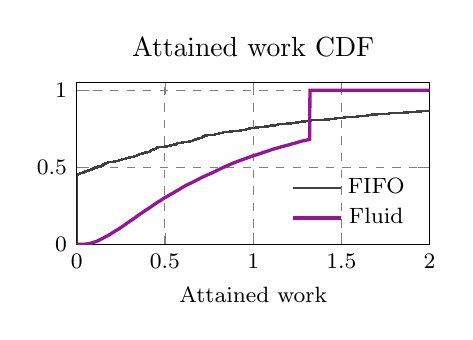
\begin{tikzpicture}
\begin{axis}[
    title=Attained work CDF,
    width=0.5\textwidth,
    height=0.3\textwidth,
    xlabel={Attained work},
    xmin=0,xmax=2.0,
    ymin=0,ymax=1.05,
    grid,
    legend pos=south east,
    ]
    \addplot[color=black!75!white, thick, solid, const plot]
        table[row sep={\\}]
        {
            \\
            0.0  0.0012484394506866417  \\
            0.0  0.0024968789013732834  \\
            0.0  0.003745318352059925  \\
            0.0  0.004993757802746567  \\
            0.0  0.006242197253433208  \\
            0.0  0.00749063670411985  \\
            0.0  0.008739076154806492  \\
            0.0  0.009987515605493134  \\
            0.0  0.011235955056179775  \\
            0.0  0.012484394506866416  \\
            0.0  0.01373283395755306  \\
            0.0  0.0149812734082397  \\
            0.0  0.016229712858926344  \\
            0.0  0.017478152309612985  \\
            0.0  0.018726591760299626  \\
            0.0  0.019975031210986267  \\
            0.0  0.02122347066167291  \\
            0.0  0.02247191011235955  \\
            0.0  0.02372034956304619  \\
            0.0  0.024968789013732832  \\
            0.0  0.026217228464419477  \\
            0.0  0.02746566791510612  \\
            0.0  0.02871410736579276  \\
            0.0  0.0299625468164794  \\
            0.0  0.031210986267166042  \\
            0.0  0.03245942571785269  \\
            0.0  0.033707865168539325  \\
            0.0  0.03495630461922597  \\
            0.0  0.03620474406991261  \\
            0.0  0.03745318352059925  \\
            0.0  0.03870162297128589  \\
            0.0  0.039950062421972535  \\
            0.0  0.04119850187265917  \\
            0.0  0.04244694132334582  \\
            0.0  0.04369538077403246  \\
            0.0  0.0449438202247191  \\
            0.0  0.046192259675405745  \\
            0.0  0.04744069912609238  \\
            0.0  0.04868913857677903  \\
            0.0  0.049937578027465665  \\
            0.0  0.05118601747815231  \\
            0.0  0.052434456928838954  \\
            0.0  0.05368289637952559  \\
            0.0  0.05493133583021224  \\
            0.0  0.056179775280898875  \\
            0.0  0.05742821473158552  \\
            0.0  0.05867665418227216  \\
            0.0  0.0599250936329588  \\
            0.0  0.06117353308364544  \\
            0.0  0.062421972534332085  \\
            0.0  0.06367041198501873  \\
            0.0  0.06491885143570537  \\
            0.0  0.066167290886392  \\
            0.0  0.06741573033707865  \\
            0.0  0.0686641697877653  \\
            0.0  0.06991260923845194  \\
            0.0  0.07116104868913857  \\
            0.0  0.07240948813982521  \\
            0.0  0.07365792759051186  \\
            0.0  0.0749063670411985  \\
            0.0  0.07615480649188515  \\
            0.0  0.07740324594257178  \\
            0.0  0.07865168539325842  \\
            0.0  0.07990012484394507  \\
            0.0  0.08114856429463171  \\
            0.0  0.08239700374531835  \\
            0.0  0.08364544319600499  \\
            0.0  0.08489388264669163  \\
            0.0  0.08614232209737828  \\
            0.0  0.08739076154806492  \\
            0.0  0.08863920099875156  \\
            0.0  0.0898876404494382  \\
            0.0  0.09113607990012484  \\
            0.0  0.09238451935081149  \\
            0.0  0.09363295880149813  \\
            0.0  0.09488139825218476  \\
            0.0  0.09612983770287141  \\
            0.0  0.09737827715355805  \\
            0.0  0.0986267166042447  \\
            0.0  0.09987515605493133  \\
            0.0  0.10112359550561797  \\
            0.0  0.10237203495630462  \\
            0.0  0.10362047440699126  \\
            0.0  0.10486891385767791  \\
            0.0  0.10611735330836454  \\
            0.0  0.10736579275905118  \\
            0.0  0.10861423220973783  \\
            0.0  0.10986267166042447  \\
            0.0  0.1111111111111111  \\
            0.0  0.11235955056179775  \\
            0.0  0.1136079900124844  \\
            0.0  0.11485642946317104  \\
            0.0  0.11610486891385768  \\
            0.0  0.11735330836454431  \\
            0.0  0.11860174781523096  \\
            0.0  0.1198501872659176  \\
            0.0  0.12109862671660425  \\
            0.0  0.12234706616729088  \\
            0.0  0.12359550561797752  \\
            0.0  0.12484394506866417  \\
            0.0  0.12609238451935081  \\
            0.0  0.12734082397003746  \\
            0.0  0.1285892634207241  \\
            0.0  0.12983770287141075  \\
            0.0  0.13108614232209737  \\
            0.0  0.132334581772784  \\
            0.0  0.13358302122347065  \\
            0.0  0.1348314606741573  \\
            0.0  0.13607990012484394  \\
            0.0  0.1373283395755306  \\
            0.0  0.13857677902621723  \\
            0.0  0.13982521847690388  \\
            0.0  0.14107365792759052  \\
            0.0  0.14232209737827714  \\
            0.0  0.14357053682896379  \\
            0.0  0.14481897627965043  \\
            0.0  0.14606741573033707  \\
            0.0  0.14731585518102372  \\
            0.0  0.14856429463171036  \\
            0.0  0.149812734082397  \\
            0.0  0.15106117353308365  \\
            0.0  0.1523096129837703  \\
            0.0  0.15355805243445692  \\
            0.0  0.15480649188514356  \\
            0.0  0.1560549313358302  \\
            0.0  0.15730337078651685  \\
            0.0  0.1585518102372035  \\
            0.0  0.15980024968789014  \\
            0.0  0.16104868913857678  \\
            0.0  0.16229712858926343  \\
            0.0  0.16354556803995007  \\
            0.0  0.1647940074906367  \\
            0.0  0.16604244694132334  \\
            0.0  0.16729088639200998  \\
            0.0  0.16853932584269662  \\
            0.0  0.16978776529338327  \\
            0.0  0.17103620474406991  \\
            0.0  0.17228464419475656  \\
            0.0  0.1735330836454432  \\
            0.0  0.17478152309612985  \\
            0.0  0.1760299625468165  \\
            0.0  0.1772784019975031  \\
            0.0  0.17852684144818975  \\
            0.0  0.1797752808988764  \\
            0.0  0.18102372034956304  \\
            0.0  0.1822721598002497  \\
            0.0  0.18352059925093633  \\
            0.0  0.18476903870162298  \\
            0.0  0.18601747815230962  \\
            0.0  0.18726591760299627  \\
            0.0  0.18851435705368288  \\
            0.0  0.18976279650436953  \\
            0.0  0.19101123595505617  \\
            0.0  0.19225967540574282  \\
            0.0  0.19350811485642946  \\
            0.0  0.1947565543071161  \\
            0.0  0.19600499375780275  \\
            0.0  0.1972534332084894  \\
            0.0  0.19850187265917604  \\
            0.0  0.19975031210986266  \\
            0.0  0.2009987515605493  \\
            0.0  0.20224719101123595  \\
            0.0  0.2034956304619226  \\
            0.0  0.20474406991260924  \\
            0.0  0.20599250936329588  \\
            0.0  0.20724094881398253  \\
            0.0  0.20848938826466917  \\
            0.0  0.20973782771535582  \\
            0.0  0.21098626716604243  \\
            0.0  0.21223470661672908  \\
            0.0  0.21348314606741572  \\
            0.0  0.21473158551810237  \\
            0.0  0.21598002496878901  \\
            0.0  0.21722846441947566  \\
            0.0  0.2184769038701623  \\
            0.0  0.21972534332084895  \\
            0.0  0.2209737827715356  \\
            0.0  0.2222222222222222  \\
            0.0  0.22347066167290885  \\
            0.0  0.2247191011235955  \\
            0.0  0.22596754057428214  \\
            0.0  0.2272159800249688  \\
            0.0  0.22846441947565543  \\
            0.0  0.22971285892634208  \\
            0.0  0.23096129837702872  \\
            0.0  0.23220973782771537  \\
            0.0  0.23345817727840198  \\
            0.0  0.23470661672908863  \\
            0.0  0.23595505617977527  \\
            0.0  0.23720349563046192  \\
            0.0  0.23845193508114856  \\
            0.0  0.2397003745318352  \\
            0.0  0.24094881398252185  \\
            0.0  0.2421972534332085  \\
            0.0  0.24344569288389514  \\
            0.0  0.24469413233458176  \\
            0.0  0.2459425717852684  \\
            0.0  0.24719101123595505  \\
            0.0  0.2484394506866417  \\
            0.0  0.24968789013732834  \\
            0.0  0.250936329588015  \\
            0.0  0.25218476903870163  \\
            0.0  0.2534332084893883  \\
            0.0  0.2546816479400749  \\
            0.0  0.25593008739076156  \\
            0.0  0.2571785268414482  \\
            0.0  0.25842696629213485  \\
            0.0  0.2596754057428215  \\
            0.0  0.26092384519350814  \\
            0.0  0.26217228464419473  \\
            0.0  0.2634207240948814  \\
            0.0  0.264669163545568  \\
            0.0  0.26591760299625467  \\
            0.0  0.2671660424469413  \\
            0.0  0.26841448189762795  \\
            0.0  0.2696629213483146  \\
            0.0  0.27091136079900124  \\
            0.0  0.2721598002496879  \\
            0.0  0.27340823970037453  \\
            0.0  0.2746566791510612  \\
            0.0  0.2759051186017478  \\
            0.0  0.27715355805243447  \\
            0.0  0.2784019975031211  \\
            0.0  0.27965043695380776  \\
            0.0  0.2808988764044944  \\
            0.0  0.28214731585518105  \\
            0.0  0.2833957553058677  \\
            0.0  0.2846441947565543  \\
            0.0  0.2858926342072409  \\
            0.0  0.28714107365792757  \\
            0.0  0.2883895131086142  \\
            0.0  0.28963795255930086  \\
            0.0  0.2908863920099875  \\
            0.0  0.29213483146067415  \\
            0.0  0.2933832709113608  \\
            0.0  0.29463171036204744  \\
            0.0  0.2958801498127341  \\
            0.0  0.29712858926342073  \\
            0.0  0.2983770287141074  \\
            0.0  0.299625468164794  \\
            0.0  0.30087390761548066  \\
            0.0  0.3021223470661673  \\
            0.0  0.30337078651685395  \\
            0.0  0.3046192259675406  \\
            0.0  0.30586766541822724  \\
            0.0  0.30711610486891383  \\
            0.0  0.3083645443196005  \\
            0.0  0.3096129837702871  \\
            0.0  0.31086142322097376  \\
            0.0  0.3121098626716604  \\
            0.0  0.31335830212234705  \\
            0.0  0.3146067415730337  \\
            0.0  0.31585518102372034  \\
            0.0  0.317103620474407  \\
            0.0  0.31835205992509363  \\
            0.0  0.3196004993757803  \\
            0.0  0.3208489388264669  \\
            0.0  0.32209737827715357  \\
            0.0  0.3233458177278402  \\
            0.0  0.32459425717852686  \\
            0.0  0.3258426966292135  \\
            0.0  0.32709113607990015  \\
            0.0  0.3283395755305868  \\
            0.0  0.3295880149812734  \\
            0.0  0.33083645443196  \\
            0.0  0.33208489388264667  \\
            0.0  0.3333333333333333  \\
            0.0  0.33458177278401996  \\
            0.0  0.3358302122347066  \\
            0.0  0.33707865168539325  \\
            0.0  0.3383270911360799  \\
            0.0  0.33957553058676654  \\
            0.0  0.3408239700374532  \\
            0.0  0.34207240948813983  \\
            0.0  0.3433208489388265  \\
            0.0  0.3445692883895131  \\
            0.0  0.34581772784019976  \\
            0.0  0.3470661672908864  \\
            0.0  0.34831460674157305  \\
            0.0  0.3495630461922597  \\
            0.0  0.35081148564294634  \\
            0.0  0.352059925093633  \\
            0.0  0.3533083645443196  \\
            0.0  0.3545568039950062  \\
            0.0  0.35580524344569286  \\
            0.0  0.3570536828963795  \\
            0.0  0.35830212234706615  \\
            0.0  0.3595505617977528  \\
            0.0  0.36079900124843944  \\
            0.0  0.3620474406991261  \\
            0.0  0.36329588014981273  \\
            0.0  0.3645443196004994  \\
            0.0  0.365792759051186  \\
            0.0  0.36704119850187267  \\
            0.0  0.3682896379525593  \\
            0.0  0.36953807740324596  \\
            0.0  0.3707865168539326  \\
            0.0  0.37203495630461925  \\
            0.0  0.3732833957553059  \\
            0.0  0.37453183520599254  \\
            0.0  0.3757802746566791  \\
            0.0  0.37702871410736577  \\
            0.0  0.3782771535580524  \\
            0.0  0.37952559300873906  \\
            0.0  0.3807740324594257  \\
            0.0  0.38202247191011235  \\
            0.0  0.383270911360799  \\
            0.0  0.38451935081148564  \\
            0.0  0.3857677902621723  \\
            0.0  0.38701622971285893  \\
            0.0  0.3882646691635456  \\
            0.0  0.3895131086142322  \\
            0.0  0.39076154806491886  \\
            0.0  0.3920099875156055  \\
            0.0  0.39325842696629215  \\
            0.0  0.3945068664169788  \\
            0.0  0.39575530586766544  \\
            0.0  0.3970037453183521  \\
            0.0  0.3982521847690387  \\
            0.0  0.3995006242197253  \\
            0.0  0.40074906367041196  \\
            0.0  0.4019975031210986  \\
            0.0  0.40324594257178525  \\
            0.0  0.4044943820224719  \\
            0.0  0.40574282147315854  \\
            0.0  0.4069912609238452  \\
            0.0  0.40823970037453183  \\
            0.0  0.4094881398252185  \\
            0.0  0.4107365792759051  \\
            0.0  0.41198501872659177  \\
            0.0  0.4132334581772784  \\
            0.0  0.41448189762796506  \\
            0.0  0.4157303370786517  \\
            0.0  0.41697877652933835  \\
            0.0  0.418227215980025  \\
            0.0  0.41947565543071164  \\
            0.0  0.4207240948813982  \\
            0.0  0.42197253433208487  \\
            0.0  0.4232209737827715  \\
            0.0  0.42446941323345816  \\
            0.0  0.4257178526841448  \\
            0.0  0.42696629213483145  \\
            0.0  0.4282147315855181  \\
            0.0  0.42946317103620474  \\
            0.0  0.4307116104868914  \\
            0.0  0.43196004993757803  \\
            0.0  0.4332084893882647  \\
            0.0  0.4344569288389513  \\
            0.0  0.43570536828963796  \\
            0.0  0.4369538077403246  \\
            0.0  0.43820224719101125  \\
            0.0  0.4394506866416979  \\
            0.0  0.44069912609238454  \\
            0.0  0.4419475655430712  \\
            0.0  0.4431960049937578  \\
            0.0  0.4444444444444444  \\
            0.0  0.44569288389513106  \\
            0.0  0.4469413233458177  \\
            0.0  0.44818976279650435  \\
            0.0  0.449438202247191  \\
            0.0  0.45068664169787764  \\
            0.002105573468128341  0.4519350811485643  \\
            0.004765421774621359  0.45318352059925093  \\
            0.006321746343957102  0.4544319600499376  \\
            0.00776056907447753  0.4556803995006242  \\
            0.01000341897464807  0.45692883895131087  \\
            0.01744145404374109  0.4581772784019975  \\
            0.019150896869817302  0.45942571785268416  \\
            0.020584811803116665  0.4606741573033708  \\
            0.02349931163254837  0.46192259675405745  \\
            0.02998841720044254  0.4631710362047441  \\
            0.033117507822993275  0.46441947565543074  \\
            0.03668690497389093  0.4656679151061174  \\
            0.03735567394696915  0.46691635455680397  \\
            0.037843996652810574  0.4681647940074906  \\
            0.03827081771896168  0.46941323345817726  \\
            0.0396036834517588  0.4706616729088639  \\
            0.042825185602779925  0.47191011235955055  \\
            0.04961319905495287  0.4731585518102372  \\
            0.053743456145127766  0.47440699126092384  \\
            0.05745841232143789  0.4756554307116105  \\
            0.06056441031393267  0.4769038701622971  \\
            0.06172402719509784  0.4781523096129838  \\
            0.06619350745500441  0.4794007490636704  \\
            0.06954701996932044  0.48064918851435706  \\
            0.07098370100982976  0.4818976279650437  \\
            0.07109105213267863  0.48314606741573035  \\
            0.07989525318642166  0.484394506866417  \\
            0.08036066753673055  0.48564294631710364  \\
            0.08637378895404879  0.4868913857677903  \\
            0.08650884036440232  0.48813982521847693  \\
            0.08801160154555987  0.4893882646691635  \\
            0.09010621934545782  0.49063670411985016  \\
            0.0940912129287419  0.4918851435705368  \\
            0.09525029384638373  0.49313358302122345  \\
            0.09742370911369846  0.4943820224719101  \\
            0.0991776321228599  0.49563046192259674  \\
            0.10214470814678833  0.4968789013732834  \\
            0.10256478222810017  0.49812734082397003  \\
            0.10628704781252907  0.4993757802746567  \\
            0.11571219260717669  0.5006242197253433  \\
            0.1159685539493438  0.50187265917603  \\
            0.12184474921531319  0.5031210986267166  \\
            0.12211482462151935  0.5043695380774033  \\
            0.1221393963226518  0.5056179775280899  \\
            0.1356462926784161  0.5068664169787765  \\
            0.13918885812279314  0.5081148564294632  \\
            0.14098257184071628  0.5093632958801498  \\
            0.1441849358787799  0.5106117353308365  \\
            0.1451385940199188  0.5118601747815231  \\
            0.1455758537640186  0.5131086142322098  \\
            0.1464693021483825  0.5143570536828964  \\
            0.14759474034792675  0.5156054931335831  \\
            0.14981045303028218  0.5168539325842697  \\
            0.1512125715631214  0.5181023720349563  \\
            0.15154336754372366  0.519350811485643  \\
            0.15437132093225614  0.5205992509363296  \\
            0.15632573887143053  0.5218476903870163  \\
            0.15643102768689232  0.5230961298377028  \\
            0.15933214280684616  0.5243445692883895  \\
            0.16447261869515728  0.5255930087390761  \\
            0.16972843357119416  0.5268414481897628  \\
            0.17185247504553303  0.5280898876404494  \\
            0.1738406284940195  0.529338327091136  \\
            0.17644768775187458  0.5305867665418227  \\
            0.17692219115976116  0.5318352059925093  \\
            0.1815883518340513  0.533083645443196  \\
            0.18571337470933713  0.5343320848938826  \\
            0.19456787169071554  0.5355805243445693  \\
            0.20433642102926797  0.5368289637952559  \\
            0.20944887549654467  0.5380774032459426  \\
            0.21462735455840232  0.5393258426966292  \\
            0.22565591521336614  0.5405742821473158  \\
            0.22647494346115948  0.5418227215980025  \\
            0.2265339066641019  0.5430711610486891  \\
            0.239052825589114  0.5443196004993758  \\
            0.24107348504103498  0.5455680399500624  \\
            0.24177070734534567  0.5468164794007491  \\
            0.24971459447142763  0.5480649188514357  \\
            0.2531978217070243  0.5493133583021224  \\
            0.2579245757063404  0.550561797752809  \\
            0.2584561477135967  0.5518102372034956  \\
            0.26034775123201825  0.5530586766541823  \\
            0.26051396055885334  0.5543071161048689  \\
            0.27347644813778516  0.5555555555555556  \\
            0.2794514854809895  0.5568039950062422  \\
            0.27956346082796557  0.5580524344569289  \\
            0.2835030384444792  0.5593008739076155  \\
            0.2967880219130876  0.5605493133583022  \\
            0.2988008975634673  0.5617977528089888  \\
            0.29928291094073245  0.5630461922596754  \\
            0.2993734542547486  0.5642946317103621  \\
            0.30126568029422174  0.5655430711610487  \\
            0.3198202272848496  0.5667915106117354  \\
            0.3210347166800318  0.568039950062422  \\
            0.3218401179000807  0.5692883895131086  \\
            0.3247439404542405  0.5705368289637952  \\
            0.3253068738715683  0.5717852684144819  \\
            0.32574932647974375  0.5730337078651685  \\
            0.3377767244288208  0.5742821473158551  \\
            0.3397908762911612  0.5755305867665418  \\
            0.3399335927292384  0.5767790262172284  \\
            0.34184941221666065  0.5780274656679151  \\
            0.34260408985306867  0.5792759051186017  \\
            0.3462943904847149  0.5805243445692884  \\
            0.34807573740519615  0.581772784019975  \\
            0.35144537674312915  0.5830212234706617  \\
            0.3529117894808351  0.5842696629213483  \\
            0.3534983803733298  0.5855181023720349  \\
            0.3641327838441555  0.5867665418227216  \\
            0.36560729195126385  0.5880149812734082  \\
            0.37047614174476706  0.5892634207240949  \\
            0.3721746771456367  0.5905118601747815  \\
            0.3763586041154987  0.5917602996254682  \\
            0.3764235706274519  0.5930087390761548  \\
            0.3868241568907749  0.5942571785268415  \\
            0.3877609935011499  0.5955056179775281  \\
            0.39525836795247926  0.5967540574282147  \\
            0.3980451670239802  0.5980024968789014  \\
            0.3995697133315157  0.599250936329588  \\
            0.4071926177061864  0.6004993757802747  \\
            0.4120711384152713  0.6017478152309613  \\
            0.4143631834867847  0.602996254681648  \\
            0.4157552913085272  0.6042446941323346  \\
            0.41772974835865284  0.6054931335830213  \\
            0.419755771688088  0.6067415730337079  \\
            0.42012061995664873  0.6079900124843945  \\
            0.42016869491715525  0.6092384519350812  \\
            0.4206034981499678  0.6104868913857678  \\
            0.42307654972231035  0.6117353308364545  \\
            0.4232072885554885  0.6129837702871411  \\
            0.42972094068707656  0.6142322097378277  \\
            0.43267108817157496  0.6154806491885143  \\
            0.4390049147085904  0.616729088639201  \\
            0.44116930941271315  0.6179775280898876  \\
            0.4449996470195572  0.6192259675405742  \\
            0.4459625941345562  0.6204744069912609  \\
            0.44828707964374814  0.6217228464419475  \\
            0.44845132609975735  0.6229712858926342  \\
            0.4486528719735192  0.6242197253433208  \\
            0.4525317065664751  0.6254681647940075  \\
            0.4530728371741475  0.6267166042446941  \\
            0.45688267075348676  0.6279650436953808  \\
            0.45985102791436816  0.6292134831460674  \\
            0.4606490749667813  0.630461922596754  \\
            0.47533372266144625  0.6317103620474407  \\
            0.4898341931262289  0.6329588014981273  \\
            0.49938809177713406  0.634207240948814  \\
            0.5110624570363527  0.6354556803995006  \\
            0.512787846489573  0.6367041198501873  \\
            0.5154672047109017  0.6379525593008739  \\
            0.5207106519521223  0.6392009987515606  \\
            0.5236874316190665  0.6404494382022472  \\
            0.5295683279710062  0.6416978776529338  \\
            0.5334527736222299  0.6429463171036205  \\
            0.5383175220425898  0.6441947565543071  \\
            0.5402496623517736  0.6454431960049938  \\
            0.5443297178256472  0.6466916354556804  \\
            0.5499339984082283  0.6479400749063671  \\
            0.5597556225157092  0.6491885143570537  \\
            0.5606718536086257  0.6504369538077404  \\
            0.5615337861202906  0.651685393258427  \\
            0.5642955213574004  0.6529338327091136  \\
            0.5665110784854086  0.6541822721598003  \\
            0.5693828204288747  0.6554307116104869  \\
            0.5703895197309166  0.6566791510611736  \\
            0.5746472421722615  0.6579275905118602  \\
            0.57964078944336  0.6591760299625468  \\
            0.5978058730557336  0.6604244694132334  \\
            0.6041207937615312  0.66167290886392  \\
            0.6156896070770312  0.6629213483146067  \\
            0.6261540687259483  0.6641697877652933  \\
            0.6309610439490356  0.66541822721598  \\
            0.6358634709262247  0.6666666666666666  \\
            0.6402339815463591  0.6679151061173533  \\
            0.6407129824937259  0.6691635455680399  \\
            0.6422625483940578  0.6704119850187266  \\
            0.6556451101325109  0.6716604244694132  \\
            0.6588623430774021  0.6729088639200999  \\
            0.6608639219624308  0.6741573033707865  \\
            0.6611718076679267  0.6754057428214731  \\
            0.6619434841090168  0.6766541822721598  \\
            0.6654936948051073  0.6779026217228464  \\
            0.6675923414468627  0.6791510611735331  \\
            0.6700937993689706  0.6803995006242197  \\
            0.6744563303755626  0.6816479400749064  \\
            0.67551076689027  0.682896379525593  \\
            0.6829534602528609  0.6841448189762797  \\
            0.6833352184538342  0.6853932584269663  \\
            0.688837160158446  0.686641697877653  \\
            0.691215678736441  0.6878901373283396  \\
            0.6961048435140498  0.6891385767790262  \\
            0.6976162575150013  0.6903870162297129  \\
            0.7049357530976295  0.6916354556803995  \\
            0.7080543211099268  0.6928838951310862  \\
            0.7090523701266278  0.6941323345817728  \\
            0.7132898679824358  0.6953807740324595  \\
            0.7140721642461896  0.6966292134831461  \\
            0.7140891098724529  0.6978776529338327  \\
            0.7150620958538242  0.6991260923845194  \\
            0.7183978151498744  0.700374531835206  \\
            0.7209726125695253  0.7016229712858927  \\
            0.7219914907074383  0.7028714107365793  \\
            0.7262264167416816  0.704119850187266  \\
            0.7284933417297594  0.7053682896379525  \\
            0.7295517881346711  0.7066167290886392  \\
            0.7404450975795385  0.7078651685393258  \\
            0.7521940648211112  0.7091136079900124  \\
            0.7526701490997709  0.7103620474406991  \\
            0.7712728887082392  0.7116104868913857  \\
            0.7820938642409772  0.7128589263420724  \\
            0.7823060765164556  0.714107365792759  \\
            0.798551542866285  0.7153558052434457  \\
            0.7988087121528893  0.7166042446941323  \\
            0.8000689397724448  0.717852684144819  \\
            0.8044999218704869  0.7191011235955056  \\
            0.8073173849576226  0.7203495630461922  \\
            0.8075646232182692  0.7215980024968789  \\
            0.8218938101190565  0.7228464419475655  \\
            0.8243652390526955  0.7240948813982522  \\
            0.8271169420135323  0.7253433208489388  \\
            0.8292547281530034  0.7265917602996255  \\
            0.835119293540231  0.7278401997503121  \\
            0.8434525052916939  0.7290886392009988  \\
            0.8597161449442439  0.7303370786516854  \\
            0.8701244010446789  0.731585518102372  \\
            0.8713723261788004  0.7328339575530587  \\
            0.8796484457159723  0.7340823970037453  \\
            0.9095821117692253  0.735330836454432  \\
            0.9196736890881139  0.7365792759051186  \\
            0.9239258664443071  0.7378277153558053  \\
            0.9264350639316932  0.7390761548064919  \\
            0.9322652087250844  0.7403245942571786  \\
            0.9455375809562305  0.7415730337078652  \\
            0.9461494973654538  0.7428214731585518  \\
            0.9538531167040247  0.7440699126092385  \\
            0.9591453356547317  0.7453183520599251  \\
            0.9592458883454356  0.7465667915106118  \\
            0.9610271941958217  0.7478152309612984  \\
            0.9677647298256451  0.7490636704119851  \\
            0.9719797882099748  0.7503121098626716  \\
            0.9785234359506774  0.7515605493133583  \\
            0.9799994189455958  0.7528089887640449  \\
            0.9906149651761496  0.7540574282147315  \\
            1.005102838694274  0.7553058676654182  \\
            1.007620469431913  0.7565543071161048  \\
            1.0160735998930193  0.7578027465667915  \\
            1.0293018081231082  0.7590511860174781  \\
            1.0355970130466234  0.7602996254681648  \\
            1.0450382359395927  0.7615480649188514  \\
            1.0662027126110296  0.762796504369538  \\
            1.070010927532394  0.7640449438202247  \\
            1.0798233956653218  0.7652933832709113  \\
            1.0849332550302928  0.766541822721598  \\
            1.0874105534814191  0.7677902621722846  \\
            1.0897575542593358  0.7690387016229713  \\
            1.0902049365858772  0.7702871410736579  \\
            1.1018828585882263  0.7715355805243446  \\
            1.1248209503690565  0.7727840199750312  \\
            1.1306817665913655  0.7740324594257179  \\
            1.1341508749807476  0.7752808988764045  \\
            1.1396147112043877  0.7765293383270911  \\
            1.1399858727042727  0.7777777777777778  \\
            1.1423229797712116  0.7790262172284644  \\
            1.1643245496132977  0.7802746566791511  \\
            1.1919502529548858  0.7815230961298377  \\
            1.1922457672918298  0.7827715355805244  \\
            1.1926855580979812  0.784019975031211  \\
            1.215172724207263  0.7852684144818977  \\
            1.223305725576186  0.7865168539325843  \\
            1.2307452251214954  0.787765293383271  \\
            1.2327412239984739  0.7890137328339576  \\
            1.2449179826403451  0.7902621722846442  \\
            1.2528738313934502  0.7915106117353309  \\
            1.2618404373137935  0.7927590511860175  \\
            1.2671216860429155  0.7940074906367042  \\
            1.2688873992267136  0.7952559300873908  \\
            1.2765886402713527  0.7965043695380774  \\
            1.2912120616559433  0.797752808988764  \\
            1.2963881397220258  0.7990012484394506  \\
            1.301588346081445  0.8002496878901373  \\
            1.3031211741467672  0.8014981273408239  \\
            1.3200618466110328  0.8027465667915106  \\
            1.3272749167971583  0.8039950062421972  \\
            1.3286920650621141  0.8052434456928839  \\
            1.348846476467612  0.8064918851435705  \\
            1.3617544286763454  0.8077403245942572  \\
            1.3835288067244425  0.8089887640449438  \\
            1.4065446483789739  0.8102372034956304  \\
            1.4292862980896786  0.8114856429463171  \\
            1.431609102368241  0.8127340823970037  \\
            1.4519583056099066  0.8139825218476904  \\
            1.4529921061959072  0.815230961298377  \\
            1.4623565335017616  0.8164794007490637  \\
            1.4671754833083905  0.8177278401997503  \\
            1.5036542730844786  0.818976279650437  \\
            1.5037646562509122  0.8202247191011236  \\
            1.5065048242138197  0.8214731585518102  \\
            1.5148278657900196  0.8227215980024969  \\
            1.520608763061034  0.8239700374531835  \\
            1.5559849173784244  0.8252184769038702  \\
            1.5630719443838994  0.8264669163545568  \\
            1.5860365752163972  0.8277153558052435  \\
            1.5890973071880055  0.8289637952559301  \\
            1.5933223763083784  0.8302122347066168  \\
            1.6003852867081036  0.8314606741573034  \\
            1.6303685164898472  0.83270911360799  \\
            1.6309662094357273  0.8339575530586767  \\
            1.635913559491187  0.8352059925093633  \\
            1.6471720728319923  0.83645443196005  \\
            1.64987482702641  0.8377028714107366  \\
            1.6656516468305043  0.8389513108614233  \\
            1.667657249404641  0.8401997503121099  \\
            1.6715994438250354  0.8414481897627965  \\
            1.676834250897926  0.8426966292134831  \\
            1.7040486794298624  0.8439450686641697  \\
            1.7059686397132623  0.8451935081148564  \\
            1.7187328512475237  0.846441947565543  \\
            1.729930954874374  0.8476903870162297  \\
            1.7699712924560327  0.8489388264669163  \\
            1.7716344876969128  0.850187265917603  \\
            1.8206910859699965  0.8514357053682896  \\
            1.8267010388969631  0.8526841448189763  \\
            1.8346551880364594  0.8539325842696629  \\
            1.8566262130041  0.8551810237203495  \\
            1.8788769484159218  0.8564294631710362  \\
            1.892687203944888  0.8576779026217228  \\
            1.8941808534899303  0.8589263420724095  \\
            1.9060864608496597  0.8601747815230961  \\
            1.9275354595349805  0.8614232209737828  \\
            1.947994680221559  0.8626716604244694  \\
            2.0106986100330455  0.8639200998751561  \\
            2.0137054974519017  0.8651685393258427  \\
            2.0184426912498097  0.8664169787765293  \\
            2.05150806752971  0.867665418227216  \\
            2.0585087776382673  0.8689138576779026  \\
            2.0681271095895464  0.8701622971285893  \\
            2.0950965673569044  0.8714107365792759  \\
            2.1049757703694216  0.8726591760299626  \\
            2.205996895854355  0.8739076154806492  \\
            2.2075812743143794  0.8751560549313359  \\
            2.2148730398892975  0.8764044943820225  \\
            2.2164952580259154  0.8776529338327091  \\
            2.233767649718572  0.8789013732833958  \\
            2.272702592965004  0.8801498127340824  \\
            2.293904406755445  0.8813982521847691  \\
            2.3101649891109295  0.8826466916354557  \\
            2.329535748091301  0.8838951310861424  \\
            2.367169079272344  0.885143570536829  \\
            2.368470648112642  0.8863920099875156  \\
            2.3718823602373553  0.8876404494382022  \\
            2.421008403510628  0.8888888888888888  \\
            2.438101030910208  0.8901373283395755  \\
            2.4669950854382137  0.8913857677902621  \\
            2.470275720243762  0.8926342072409488  \\
            2.4704734575576377  0.8938826466916354  \\
            2.4906248233107453  0.8951310861423221  \\
            2.4961398309895904  0.8963795255930087  \\
            2.511413687566069  0.8976279650436954  \\
            2.514031430278663  0.898876404494382  \\
            2.5597780649408266  0.9001248439450686  \\
            2.567392660447128  0.9013732833957553  \\
            2.5733877651570785  0.9026217228464419  \\
            2.592609319869758  0.9038701622971286  \\
            2.5956492440095604  0.9051186017478152  \\
            2.6147145304970847  0.9063670411985019  \\
            2.625481073548855  0.9076154806491885  \\
            2.636903781649642  0.9088639200998752  \\
            2.6649810645627094  0.9101123595505618  \\
            2.665584529787168  0.9113607990012484  \\
            2.6678518142864074  0.9126092384519351  \\
            2.6807898627565274  0.9138576779026217  \\
            2.729816228781882  0.9151061173533084  \\
            2.746478340015199  0.916354556803995  \\
            2.815259303693473  0.9176029962546817  \\
            2.824133890256562  0.9188514357053683  \\
            2.848073202159454  0.920099875156055  \\
            2.929831499891453  0.9213483146067416  \\
            2.9435965965713535  0.9225967540574282  \\
            3.009174869857051  0.9238451935081149  \\
            3.0437438046820637  0.9250936329588015  \\
            3.0586047752464403  0.9263420724094882  \\
            3.0996230173645216  0.9275905118601748  \\
            3.137403015108397  0.9288389513108615  \\
            3.146786181345772  0.9300873907615481  \\
            3.1653574392694424  0.9313358302122348  \\
            3.1666801816354866  0.9325842696629213  \\
            3.2056461557102702  0.9338327091136079  \\
            3.2817692157173535  0.9350811485642946  \\
            3.30187790712327  0.9363295880149812  \\
            3.312422682004342  0.9375780274656679  \\
            3.339994606015566  0.9388264669163545  \\
            3.363443804073696  0.9400749063670412  \\
            3.461868896730251  0.9413233458177278  \\
            3.5082577273516797  0.9425717852684145  \\
            3.5857847165541212  0.9438202247191011  \\
            3.6211748376328856  0.9450686641697877  \\
            3.6222987272720157  0.9463171036204744  \\
            3.6732914485871606  0.947565543071161  \\
            3.734347327486682  0.9488139825218477  \\
            3.759240861052092  0.9500624219725343  \\
            3.769876956985826  0.951310861423221  \\
            3.8108504655268955  0.9525593008739076  \\
            3.8584427676817796  0.9538077403245943  \\
            3.8714810216826585  0.9550561797752809  \\
            3.89540203251849  0.9563046192259675  \\
            3.941685240011104  0.9575530586766542  \\
            3.99108766177644  0.9588014981273408  \\
            4.023843551215045  0.9600499375780275  \\
            4.046408493159545  0.9612983770287141  \\
            4.088253949767775  0.9625468164794008  \\
            4.318968364229496  0.9637952559300874  \\
            4.446696731419758  0.9650436953807741  \\
            4.458894382435275  0.9662921348314607  \\
            4.460987633280077  0.9675405742821473  \\
            4.550878693917297  0.968789013732834  \\
            4.557711862020208  0.9700374531835206  \\
            4.874563284613394  0.9712858926342073  \\
            4.925006209144636  0.9725343320848939  \\
            5.089483103310337  0.9737827715355806  \\
            5.0925900803534265  0.9750312109862672  \\
            5.143962573787122  0.9762796504369539  \\
            5.1636063543828135  0.9775280898876404  \\
            5.24250407789369  0.978776529338327  \\
            5.458792588391227  0.9800249687890137  \\
            5.479553703558786  0.9812734082397003  \\
            5.54272398286852  0.982521847690387  \\
            5.746158182895226  0.9837702871410736  \\
            6.712608522565221  0.9850187265917603  \\
            7.138323369336647  0.9862671660424469  \\
            7.1918285608070835  0.9875156054931336  \\
            7.293983424304409  0.9887640449438202  \\
            7.505491202828763  0.9900124843945068  \\
            8.029067634104692  0.9912609238451935  \\
            8.108427416325286  0.9925093632958801  \\
            8.334830525955223  0.9937578027465668  \\
            8.342072076949272  0.9950062421972534  \\
            8.489620452181695  0.9962546816479401  \\
            8.598483986274335  0.9975031210986267  \\
            10.867223548613552  0.9987515605493134  \\
            15.873150722018503  1.0  \\
        }
        ;
    \addlegendentry {FIFO}
    \addplot[color=violetita,solid, very thick]
        table[row sep={\\}]
        {
            \\
            0.0  0.0  \\
            0.01  0.0  \\
            0.02  0.0001  \\
            0.03  0.0003  \\
            0.04  0.00105  \\
            0.05  0.0021  \\
            0.06  0.00335  \\
            0.07  0.0054  \\
            0.08  0.0074  \\
            0.09  0.0111  \\
            0.1  0.0148  \\
            0.11  0.019  \\
            0.12  0.02355  \\
            0.13  0.02935  \\
            0.14  0.035  \\
            0.15  0.0411  \\
            0.16  0.04725  \\
            0.17  0.05325  \\
            0.18  0.0589  \\
            0.19  0.0661  \\
            0.2  0.074  \\
            0.21  0.0804  \\
            0.22  0.0878  \\
            0.23  0.0945  \\
            0.24  0.101  \\
            0.25  0.10945  \\
            0.26  0.11695  \\
            0.27  0.12475  \\
            0.28  0.1337  \\
            0.29  0.1413  \\
            0.3  0.14995  \\
            0.31  0.1568  \\
            0.32  0.1652  \\
            0.33  0.1724  \\
            0.34  0.18125  \\
            0.35  0.18975  \\
            0.36  0.19775  \\
            0.37  0.20475  \\
            0.38  0.2128  \\
            0.39  0.221  \\
            0.4  0.2282  \\
            0.41  0.2348  \\
            0.42  0.24325  \\
            0.43  0.25125  \\
            0.44  0.2589  \\
            0.45  0.26695  \\
            0.46  0.27445  \\
            0.47  0.28145  \\
            0.48  0.289  \\
            0.49  0.2968  \\
            0.5  0.30315  \\
            0.51  0.3096  \\
            0.52  0.31605  \\
            0.53  0.3228  \\
            0.54  0.32895  \\
            0.55  0.33565  \\
            0.56  0.34335  \\
            0.57  0.3489  \\
            0.58  0.3557  \\
            0.59  0.36335  \\
            0.6  0.3703  \\
            0.61  0.37665  \\
            0.62  0.38365  \\
            0.63  0.38875  \\
            0.64  0.3942  \\
            0.65  0.3993  \\
            0.66  0.4053  \\
            0.67  0.41065  \\
            0.68  0.41725  \\
            0.69  0.42295  \\
            0.7  0.4289  \\
            0.71  0.43455  \\
            0.72  0.4403  \\
            0.73  0.44495  \\
            0.74  0.4502  \\
            0.75  0.45545  \\
            0.76  0.45985  \\
            0.77  0.46545  \\
            0.78  0.4707  \\
            0.79  0.4771  \\
            0.8  0.4821  \\
            0.81  0.4877  \\
            0.82  0.49345  \\
            0.83  0.499  \\
            0.84  0.50385  \\
            0.85  0.50885  \\
            0.86  0.5138  \\
            0.87  0.51935  \\
            0.88  0.5239  \\
            0.89  0.52895  \\
            0.9  0.5328  \\
            0.91  0.53735  \\
            0.92  0.54165  \\
            0.93  0.5456  \\
            0.94  0.5498  \\
            0.95  0.55395  \\
            0.96  0.5583  \\
            0.97  0.5622  \\
            0.98  0.56615  \\
            0.99  0.5711  \\
            1.0  0.57465  \\
            1.01  0.57835  \\
            1.02  0.5815  \\
            1.03  0.58565  \\
            1.04  0.5892  \\
            1.05  0.5932  \\
            1.06  0.59725  \\
            1.07  0.60065  \\
            1.08  0.60485  \\
            1.09  0.60825  \\
            1.1  0.61255  \\
            1.11  0.61645  \\
            1.12  0.61975  \\
            1.13  0.6228  \\
            1.14  0.62605  \\
            1.15  0.62905  \\
            1.16  0.63315  \\
            1.17  0.6361  \\
            1.18  0.6389  \\
            1.19  0.64225  \\
            1.2  0.64475  \\
            1.21  0.648  \\
            1.22  0.6517  \\
            1.23  0.6549  \\
            1.24  0.6573  \\
            1.25  0.66095  \\
            1.26  0.66465  \\
            1.27  0.6679  \\
            1.28  0.67095  \\
            1.29  0.67315  \\
            1.3  0.6756  \\
            1.31  0.6786  \\
            1.32  0.6813  \\
            1.322  1.0  \\
            3.0  1.0  \\
        }
        ;
    \addlegendentry {Fluid}
\end{axis}
\end{tikzpicture}

% 	\end{center}

% 	\vfill

% 	Almost 80\% of the jobs leave without service.
% \end{frame}

\section{Final remarks}

\begin{frame}{Messages from the talk}
	
	\begin{myitem}
		\item Measure-valued processes are a powerful tool to model general service queues.
		\item Partial service queues require two-dimensional measures.
		\item Our proposed dynamics for fluid models are tractable and approximate the real system.
		\item Last-but-not-least: in this setting, \alert{deadline-oblivious} policies can be used without performance penalty!
	\end{myitem}
\end{frame}

\begin{frame}{Future work}
	
	\begin{myitem}
		\item Analyze further policies using these tools (FCFS is easy for instance).
		\item Establish process-level convergence to the fluid models (almost done!)
		\item Devise new policies and/or analyze different settings:
		
		\begin{itemize}
			\item Tasks stay until service completion, but we want to measure the average \emph{tardiness}, i.e. how late they depart.
		\end{itemize}
	\end{myitem}
\end{frame}


\begin{frame}[plain]
	\vfill
	{\Huge \alert{Thank you!}}
	\vfill
	Andres Ferragut

	\smallskip

	\href{mailto://ferragut@ort.edu.uy}{\alert{ferragut@ort.edu.uy}}
	
	\smallskip

	\href{http://aferragu.github.io}{\alert{https://aferragu.github.io}}
\end{frame}

\begin{frame}[allowframebreaks]{References}
	\bibliography{reneging}
\end{frame}
\end{document}
